\chapter{Oligopoly with Differentiated Products}\label{ch:diffprod}

Breakfast cereals, automobiles, airline tickets and prescription drugs are each sold by a handful of firms. Each
firm offers several products, and consumers do not regard any two of them as perfect substitutes. Markets like
these are the main subject of empirical industrial organization. The tools of \cref{ch:theory,ch:conduct} were
built for a homogeneous good, with one price, an obvious set of competitors and a single conduct parameter. With
differentiated products every product has its own price, and the boundary of the market is a matter of degree.
Market power then depends on the whole matrix of own and cross price effects. This chapter develops the theory of
price competition in such markets. It also assembles the toolkit that later chapters use to measure market power,
simulate mergers and value new goods.

The organizing object is the first-order condition of a multi-product firm. It links the demand system, the
ownership of products, prices and marginal costs. In matrix form it inverts into the markup formula
$p = mc - (\Omega \odot \Delta^\top)^{-1}q$. The \emph{ownership matrix} $\Omega$ records which products each firm
prices jointly, and $\Delta$ collects the price derivatives of demand. Almost every empirical model in this book
closes its supply side with this formula. Once demand has been estimated, the formula recovers marginal costs
without accounting data. Changing $\Omega$ or costs and solving the formula again yields counterfactual prices
after a merger, a tax or the entry of a product.

The chapter has two halves. The first takes demand as given and studies the supply side. \Cref{sec:04-why}
explains why differentiation is the normal case and which questions require a demand system.
\Cref{sec:04-bertrand} derives the multi-product Bertrand-Nash pricing conditions, inverts them for markups and
works through linear and logit examples. \Cref{sec:04-diversion} rewrites the pricing rule in terms of diversion
ratios, the quantities that govern the unilateral effects of mergers. \Cref{sec:04-existence} asks when a price
equilibrium exists, when it is unique and what happens when it is not, with a full treatment of the existence
theorem of \citet{CaplinNalebuff1991}. \Cref{sec:04-supply} puts the pricing rule to work. It recovers marginal
costs, compares models of conduct, computes counterfactuals and derives pass-through.

The second half turns to the choice of demand system. \Cref{sec:04-spaces} contrasts demand written over products
with demand written over product characteristics, and it shows how the dimension of the characteristics space
shapes competition. \Cref{sec:04-repcons} studies the linear, constant elasticity of substitution (CES) and logit systems, which tame the dimensionality
of product space by imposing symmetry. It derives their representative-consumer and discrete-choice foundations,
the theme of the book by \citet{AndersonDePalmaThisse1992}. A two-sector CES model of monopolistic competition then
asks whether markets supply the right number of products. \Cref{sec:04-location} develops the location models of
\citet{Hotelling1929} and \citet{Salop1979}, a symmetric oligopoly with i.i.d.\ tastes and the vertical model of
quality choice. These models add product choice and entry to price competition. They also show when free entry
yields too many products.

A simulated market of 25 logit products owned by five firms runs through the chapter. We compute its equilibrium
in \cref{ex:04-logit25} and verify that the equilibrium is unique in \cref{ex:04-logit25-unique}. We then recover
its costs under alternative models of conduct (\cref{ex:04-mc-recovery}) and simulate a merger in it
(\cref{ex:04-merger-sim}). Two smaller examples recur as well. A linear duopoly has closed-form solutions
(\cref{ex:04-linear-duopoly}), and a logit duopoly with two consumer segments has two equilibria
(\cref{ex:04-multiple-eq}).

The chapter builds on \cref{ch:theory}, whose monopoly pricing rule, Bertrand paradox and pass-through formulas
reappear here product by product. It replaces the conduct parameter of \cref{ch:conduct} with an ownership matrix
and shows how the two are related (\cref{rem:04-kappa-theta}). The rest of the book uses its results throughout.
The demand systems of \cref{ch:aids,ch:discrete,ch:logit,ch:blp} supply the derivatives in $\Delta$, and
\cref{ch:blp,ch:airlines} estimate demand and costs together. Upward pricing pressure and merger simulation in
\cref{ch:mergers} apply \cref{sec:04-diversion,sec:04-supply} directly. Full collusion corresponds to a matrix
$\Omega$ of ones, the benchmark of \cref{ch:collusion-theory}. \Cref{sec:B-fixedpoint,sec:B-ift} collect the contraction mapping and
implicit function theorems used in the proofs, and \cref{app:problems} returns to the 25-product market as a
worked problem.

\section{Why product differentiation matters}\label{sec:04-why}

This section explains why differentiation is the normal case, which economic questions it raises, and how theory
and empirical work divide the resulting problem between them.

\subsection{Differentiation is the rule}\label{sec:04-why-rule}

Products are \emph{differentiated} when consumers do not regard them as perfect substitutes. Products differ in
physical characteristics (horsepower, sugar content, screen size) and in location (a gasoline station on one
corner or the next). They also differ in brand and reputation, in the service that comes with them, and in timing
(a morning or an evening flight). Two consumers facing the same prices often buy different products. The same consumer may switch
products when relative prices change, but not all of her demand moves at once.

Differentiation appears even in markets that look homogeneous. A branded drug and its generic version are
chemically identical, yet the branded version keeps a large share at a much higher price. Gasoline is a
standardized commodity, yet stations differ in location, brand and amenities, and nearby stations compete far
more intensely than distant ones. Near-homogeneous markets exist, but they are rare. Wholesale electricity and
refined sugar are two examples, and they are the settings of \citet{Wolfram1999} and
\citet{GenesoveMullin1998}, studied in \cref{ch:conduct}.

Differentiation changes the objects that describe a market. Let $q_j(p)$ be the demand for product $j$ as a
function of the whole price vector $p = (p_1, \dots, p_J)^\top$. Three consequences follow.
\begin{enumerate}[label=(\roman*)]
  \item There is no single market price. There is a vector of prices, one for each product, and these prices can
  differ persistently.
  \item There is no natural boundary of the market. Every product substitutes for many others to some degree, so
  the set of ``competitors'' is a matter of degree.
  \item The own-price elasticity of product $j$,
  \begin{equation*}
  \varepsilon_j(p) = -\frac{\partial q_j(p)}{\partial p_j}\frac{p_j}{q_j(p)},
  \end{equation*}
  depends on rivals' prices and on how close rival products are in the eyes of consumers. Market power is no
  longer summarized by one elasticity. It depends on the whole matrix of own and cross effects.
\end{enumerate}
Differentiation also resolves a puzzle from \cref{ch:theory}. With a homogeneous good, two price-setting firms
with equal constant costs drive price down to marginal cost (\cref{prop:02-bertrand}). The reason is that a
small price cut captures the whole market, so demand is discontinuous in prices. With differentiated products a
small price cut attracts only the marginal consumers, demand is continuous, and price competition among a few
firms leaves positive margins.

\subsection{Questions that require a demand system}\label{sec:04-why-questions}

A \emph{demand system} is the vector of demand functions $q(p, z) = (q_1(p, z), \dots, q_J(p, z))^\top$ for all
$J$ products, as functions of all prices $p$ and of demand shifters $z$ (characteristics, income, season). Many
central questions of industrial organization cannot be answered without one. \Cref{tab:04-questions} lists five
of them with the object each requires. We discuss each in turn.

\begin{table}[htbp]
\centering
\caption{Questions about differentiated-product markets and the demand objects they require}
\label{tab:04-questions}
\footnotesize
\begin{tabularx}{\textwidth}{@{}>{\raggedright\arraybackslash}p{3.3cm}X>{\raggedright\arraybackslash}p{2.6cm}@{}}
\toprule
Question & Demand object required & Treated in \\
\midrule
Measuring market power & Own and cross price derivatives at observed prices, plus a model of price setting
& \cref{sec:04-bertrand,sec:04-supply} \\[2pt]
Welfare effects of mergers & Diversion between the merging products and their margins, or the full system for
simulation & \cref{sec:04-diversion}, \cref{ch:mergers} \\[2pt]
Effects of taxes and tariffs & Pass-through, which depends on second derivatives of demand and on strategic
responses & \cref{prop:04-passthrough}, \cref{ch:theory} \\[2pt]
Product introduction and positioning & Demand for products not yet sold, so tastes over characteristics &
\cref{sec:04-spaces,sec:04-location} \\[2pt]
Welfare from new goods and price indices & Demand far from observed prices, up to the price at which demand for
the new good is zero & \cref{ch:newgoods} \\
\bottomrule
\end{tabularx}
\end{table}

\casehead{Measuring market power}
Accounting data rarely measure marginal cost (\cref{ch:intro}). The approach of the New Empirical Industrial
Organization \citep{Bresnahan1989} infers markups from behavior instead. With differentiated products this
requires the own and cross price derivatives of demand at observed prices and a model of how firms set prices.
Given both, \cref{sec:04-bertrand-matrix} shows that markups follow from a matrix inversion, and
\cref{sec:04-supply} turns them into estimates of marginal cost.

\casehead{Mergers}
A merger of two sellers of substitutes raises prices when the merged firm internalizes the sales that each product
loses to the other. The size of this effect depends on the share of one product's lost customers who would switch
to the other, a quantity called the diversion ratio (\cref{sec:04-diversion}). It also depends on the margins
earned on those customers. Predicting post-merger prices requires the full demand system and a model of supply
(\cref{sec:04-counterfactuals}, \cref{ch:mergers}).

\casehead{Taxes and tariffs}
The incidence of a tax or tariff depends on how much of a cost increase firms pass on to prices. In
\cref{ch:theory} pass-through depends on the curvature of demand. With differentiated products it also depends on
how rivals respond to one another's price changes. This requires second derivatives of the demand system
(\cref{prop:04-passthrough}).

\casehead{Product introduction}
Whether a firm should launch a new product depends on how many sales the product takes from rivals and how many it
takes from the firm's own products. Answering this before launch requires a model that predicts demand for a
product nobody has bought yet. This pushes us toward demand defined over product characteristics
(\cref{sec:04-spaces}) and toward models of product choice (\cref{sec:04-location}).

\casehead{New goods and price indices}
A consumer price index that ignores new goods overstates the increase in the cost of living. Valuing a new good
requires the price at which its demand would be zero, the \emph{virtual price}, and the area under the demand
curve above the observed price. \citet{Hausman1997} computes it for a new breakfast cereal from an estimated
demand system (\cref{ch:newgoods}). The calculation extrapolates demand far from observed prices, so it depends
heavily on functional form.

\subsection{Demand systems and market definition}\label{sec:04-why-market}

In a homogeneous-good industry the market is the set of sellers of the identical good, and concentration
measures such as the Herfindahl index $\HHI = \sum_i s_i^2$ are computed on it (\cref{ch:intro},
\cref{sec:02-concentration}). With differentiated products this boundary does not exist, yet antitrust practice
still needs one. Agencies and courts draw it with the \emph{hypothetical monopolist test}. Imagine a
profit-maximizing firm that owned every product in a candidate set. The set is a relevant market if this firm would
impose a \emph{small but significant and non-transitory increase in price} (SSNIP) on at least one of them. The SSNIP is
usually taken to be 5 or 10 percent \citep[footnote 58]{FarrellShapiro2010}. Page, footnote and inequality numbers
for \citet{FarrellShapiro2010} refer to its 2008 working-paper version. Starting from the products of the merging
firms, the analyst adds the next-closest substitutes until the test is passed (\cref{sec:11-hmt}).

Whether a SSNIP is profitable is a question about the demand system. When the hypothetical monopolist raises the
price of one product in the set, some of the lost customers switch to other products in the set and are
recaptured. The test therefore depends on own and cross elasticities or, equivalently, on diversion ratios. Let
the price rise by a fraction $X$, let $\bar m = \frac{p - mc}{p}$ be the percentage margin, and let $\ell$ be the
fraction of unit sales lost (both symbols are local to this subsection). Profit per dollar of initial revenue
moves from $\bar m$ to $(X + \bar m)(1 - \ell)$. The increase is unprofitable exactly when
\begin{align*}
(X + \bar m)(1 - \ell) < \bar m
&\iff X - (X + \bar m)\,\ell < 0 \\
&\iff \ell > \frac{X}{X + \bar m}.
\end{align*}
The threshold $\frac{X}{X + \bar m}$ is the \emph{break-even loss}, the largest loss of sales that leaves the
increase profitable. With $X = 0.05$ and $\bar m = 0.45$ it equals $\frac{0.05}{0.50} = 0.10$. High margins make
the break-even loss small. \Cref{sec:11-critloss} derives the actual loss from demand, compares the two numbers
and explains why high margins can make the test misleading.

A fully specified demand system makes market definition a by-product. Once we know how each price affects each
quantity, we can compute the price effects of a merger directly. Upward pricing pressure needs only diversion
ratios and margins (\cref{sec:04-diversion}). Merger simulation solves for the new equilibrium
(\cref{sec:04-counterfactuals}, \cref{ch:mergers}). Neither requires a decision about which products are ``in''
the market.

Concentration still plays a central role in practice. The 1992 Horizontal Merger Guidelines \citep{USDOJFTC1992}
set a presumption in Section 1.51(c), which \citet[p.~26]{FarrellShapiro2010} quote. When the post-merger HHI
exceeds 1800, a merger that raises the HHI by more than 100 points is presumed likely to create or enhance market
power or facilitate its exercise. A merger of two of seven symmetric firms raises
the HHI from 1,429 to 1,837 and so meets this presumption (same page). The 2010 Horizontal Merger Guidelines
\citep{USDOJFTC2010} keep safe harbors and presumptions of harm that depend on both the post-merger HHI and its
change \citep[p.~226]{AskerNocke2021}. \Cref{ch:mergers} compares the thresholds of the 1992 and 2010 Guidelines and
of the 2023 Merger Guidelines \citep{USDOJFTC2023} in \cref{tab:11-guidelines}, and it studies how well such
screens predict merger effects.

\subsection{How theory and empirical work divide the problem}\label{sec:04-why-division}

The theory of imperfect competition began with homogeneous goods. \citet{Cournot1838} solved for the equilibrium
outputs of firms producing an identical good. \citet{Bertrand1883} objected that price is the natural strategic
variable, and with identical goods price competition drives price to marginal cost. \citet{Edgeworth1897} showed
that capacity constraints can destroy the existence of a pure-strategy price equilibrium.
\citet{Hotelling1929} then argued that imperfect substitutability softens price competition, because a firm does
not take all its rivals' business by undercutting slightly. His model of firms located along a street is the
first model of product differentiation. It also exposed the main technical difficulty of the field. A firm may
prefer either a high price aimed at the consumers who like its product most or a low price aimed at the mass
market to any intermediate price. Profit is then not \emph{quasi-concave} in own price, meaning that its upper
contour sets are not intervals. A pure-strategy price equilibrium can then fail to exist
\citep[pp.~1--3 of the discussion-paper version]{CaplinNalebuff1991}.

The theory of differentiated products that grew from these beginnings studies mainly the supply side. Given a
demand system, which prices and which products arise in equilibrium? Representative contributions are the
discrete-choice foundations of \citet{AndersonDePalmaThisse1992}, the models of quality competition of
\citet{ShakedSutton1982,ShakedSutton1983}, and the existence results of \citet{CaplinNalebuff1991}. This theory has
two branches. The first studies price competition among a given set of products. Caplin and Nalebuff provide
conditions for existence of equilibrium that cover a wide class of demand models (\cref{sec:04-existence}). The
second studies competition in product space, in which firms choose locations or qualities, with or without
subsequent price competition. Examples are Hotelling's line, the circle of \citet{Salop1979}, and quality
ladders. Empirical work concentrates almost entirely on the first branch. We study the second in
\cref{sec:04-location}, and much room remains for empirical work on it.

Empirical work, in turn, concentrates on the demand side. There are three reasons. Prices, quantities and product
characteristics are observed far more often than costs, so the data speak most directly to demand. The supply
model can be general, because the same pricing rule applies across industries once demand is known. And demand
for differentiated products is complex enough to absorb most of the modeling effort. The supply side is therefore
modeled simply, almost always as the static multi-product Bertrand-Nash game of \cref{sec:04-bertrand}. This is
why we develop supply first. It is nearly identical across applications, and it shows which features of demand
matter for the questions of \cref{sec:04-why-questions}.

In some industries demand is the natural object even without a supply model. Electricity distribution, water,
postal services and parts of health care set prices through regulation or other non-market mechanisms. Price
there is a policy choice rather than an equilibrium outcome. To evaluate a change in a regulated price we need
the demand response and the resulting change in consumer welfare, but no model of price setting.

Demand aggregates the choices of many individuals, and each of us can introspect about our own choices. This
invites ever richer models: more heterogeneity, more characteristics, more realistic substitution. We should
resist the pull and treat added richness as an investment with costs and benefits. Richer models carry more
assumptions, which are harder to test. They are harder to compute and to estimate reliably. They are also harder
to communicate to the courts, agencies and managers who use the results.

The benefit of richness is what it buys for the question at hand. If a richer model changes the answer to the
question we are asking, and the data can discipline its extra parameters, the cost is worth paying. If the added
value is small, a simpler and less realistic model can be the better tool. A model should always be judged
against the question it is meant to answer and the data available to answer it. This principle guides the
choices among demand models in the remainder of the book. The rest of this chapter follows the division just
described: supply first (\cref{sec:04-bertrand,sec:04-diversion,sec:04-existence,sec:04-supply}), then the choice
of demand system (\cref{sec:04-spaces,sec:04-repcons,sec:04-location}).

\section{Multi-product Bertrand-Nash pricing}\label{sec:04-bertrand}

This section develops the supply model that every later chapter uses. Firms own several products and set all
their prices simultaneously, taking rivals' prices as given. We derive the first-order conditions, write them in
matrix form, invert them for markups, and work through linear and logit examples. The section ends with a
numerical market of 25 logit products that we revisit later in the book.

\subsection{Environment and equilibrium}\label{sec:04-bertrand-setup}

\begin{assumption}[Multi-product price competition]\label{ass:04-bertrand}
\leavevmode
\begin{enumerate}[label=(\alph*)]
  \item \emph{Products.} There are $J$ inside products, $j = 1, \dots, J$, and an outside good $j = 0$ whose price
  is normalized to zero.
  \item \emph{Ownership.} There are $F$ firms. Firm $f$ owns the set of products $\mathcal{J}_f$, the sets
  $\mathcal{J}_1, \dots, \mathcal{J}_F$ partition $\{1, \dots, J\}$, and $f(j)$ denotes the owner of product
  $j$.
  \item \emph{Demand.} Demand for product $j$ is $q_j(p) = M s_j(p)$, with market size $M$ and share $s_j(p)$.
  On an open set $\mathcal{P}$ of price vectors each $q_j$ is twice continuously differentiable and positive,
  $\frac{\partial q_j}{\partial p_j} < 0$, and $\frac{\partial q_k}{\partial p_j} \ge 0$ for all $k \ne j$,
  including the outside good. Products are \emph{gross substitutes}.
  \item \emph{Costs.} Product $j$ has a cost function $C_j(q_j)$ that is increasing and differentiable, with
  marginal cost $mc_j(q_j) = C_j'(q_j)$. Costs are separable across products.
  \item \emph{Timing and information.} Firms know demand and costs. They choose prices simultaneously, once,
  and then serve all the demand at those prices.
\end{enumerate}
\end{assumption}

We write $p_{\mathcal{J}_f}$ for the vector of firm $f$'s prices and $p_{-\mathcal{J}_f}$ for the prices of all
other products. Firm $f$'s profit is
\begin{equation}\label{eq:04-profit}
\pi_f(p) = \sum_{k \in \mathcal{J}_f}\Big[p_k\,q_k(p) - C_k\big(q_k(p)\big)\Big].
\end{equation}

\begin{definition}[Bertrand-Nash equilibrium]\label{def:04-bertrand-nash}
The \emph{best response} of firm $f$ to rivals' prices is the set
$BR_f(p_{-\mathcal{J}_f}) = \argmax_{p_{\mathcal{J}_f}}\pi_f(p_{\mathcal{J}_f}, p_{-\mathcal{J}_f})$. A price vector
$p^*$ is a \emph{Bertrand-Nash equilibrium} if, for every firm $f$ and every $p_{\mathcal{J}_f}$,
\begin{equation*}
\pi_f\big(p^*_{\mathcal{J}_f}, p^*_{-\mathcal{J}_f}\big) \ge \pi_f\big(p_{\mathcal{J}_f}, p^*_{-\mathcal{J}_f}\big).
\end{equation*}
Equivalently, $p^*_{\mathcal{J}_f} \in BR_f(p^*_{-\mathcal{J}_f})$ for every $f$, so $p^*$ is a fixed point of
the joint best-response map.
\end{definition}

Is price setting a sensible description of conduct? In many differentiated-product markets firms post prices and
then sell whatever consumers demand at those prices. Cars, consumer electronics and breakfast cereals fit this
description. Differentiation also removes the Bertrand paradox of \cref{prop:02-bertrand}, so the model
predicts positive margins with few firms. With differentiated products, price and quantity competition lead to
different outcomes, and price competition yields lower prices when the goods are substitutes
\citep{SinghVives1984}.

The model fits less well when firms commit to capacity before they set prices and capacity binds.
\Cref{prop:02-ks} shows, following \citet{KrepsScheinkman1983}, that capacity choice followed by price
competition can reproduce Cournot outcomes with a homogeneous good. The right model then depends on the timing of
commitments and on whether capacity is slack. The model is also static. It ignores repeated interaction, which
can sustain higher prices (\cref{ch:collusion-theory}), and it ignores costs of adjusting prices.

Assuming Bertrand-Nash conduct is a choice of the analyst. \Cref{ch:conduct} treated conduct as an unknown
parameter $\theta$ to be estimated. The differentiated-products literature instead imposes Nash pricing and
spends its identifying power on demand. The assumption can still be tested. Alternative models of conduct
correspond to alternative ownership matrices in the pricing equations below, and \cref{sec:04-supply} compares
them.

\subsection{The first-order conditions}\label{sec:04-bertrand-foc}

We derive the first-order condition of firm $f$ for the price of one of its products, $p_j$ with
$j \in \mathcal{J}_f$. Rivals' prices are held fixed, as the Nash assumption requires. Write the profit
\eqref{eq:04-profit} with the summation index $k$, so that $j$ is free to denote the price being changed. Profit
is a sum of revenue terms $p_k q_k(p)$ and cost terms $C_k(q_k(p))$. The product rule applied to a revenue term
gives
\begin{equation*}
\frac{\partial}{\partial p_j}\big[p_k\,q_k(p)\big] = \indic\{k = j\}\,q_k(p) + p_k\,\frac{\partial q_k(p)}{\partial p_j},
\end{equation*}
because $p_k$ depends on $p_j$ only when $k = j$. The chain rule applied to a cost term gives
\begin{equation*}
\frac{\partial}{\partial p_j}C_k\big(q_k(p)\big) = mc_k(q_k)\,\frac{\partial q_k(p)}{\partial p_j}.
\end{equation*}
Summing over $k \in \mathcal{J}_f$ and subtracting the cost terms from the revenue terms,
\begin{equation*}
\frac{\partial \pi_f(p)}{\partial p_j}
= q_j(p) + \sum_{k \in \mathcal{J}_f} p_k\frac{\partial q_k(p)}{\partial p_j}
- \sum_{k \in \mathcal{J}_f} mc_k(q_k)\frac{\partial q_k(p)}{\partial p_j}.
\end{equation*}
Collecting the two sums and setting the derivative to zero gives the first-order condition
\begin{equation}\label{eq:04-foc-scalar}
q_j(p) + \sum_{k \in \mathcal{J}_f}\big(p_k - mc_k\big)\frac{\partial q_k(p)}{\partial p_j} = 0,
\qquad j \in \mathcal{J}_f.
\end{equation}

We call $m_j = p_j - mc_j$ the (dollar) \emph{markup} of product $j$ and $m = (m_1, \dots, m_J)^\top$ the vector
of markups. Separating the term $k = j$ from the others, \eqref{eq:04-foc-scalar} reads
\begin{equation*}
\underbrace{q_j}_{\text{inframarginal gain}}
+ \underbrace{m_j\frac{\partial q_j}{\partial p_j}}_{\text{lost margin}}
+ \underbrace{\sum_{k \in \mathcal{J}_f\setminus\{j\}} m_k\frac{\partial q_k}{\partial p_j}}_{\text{recaptured margin}}
= 0.
\end{equation*}
Each term has an economic meaning. A one-dollar increase in $p_j$ earns one more dollar on each of the $q_j$
units still sold. It loses the margin $m_j$ on each of the $-\frac{\partial q_j}{\partial p_j}$ buyers who stop
buying product $j$. Some of those buyers switch to the firm's other products, and the firm earns $m_k$ on each of
the $\frac{\partial q_k}{\partial p_j}$ who switch to product $k$. A single-product firm has no third term. A
multi-product firm internalizes the \emph{cannibalization} among its own products, so the third term makes
raising $p_j$ more attractive.

There is one condition per product, so \eqref{eq:04-foc-scalar} is a system of $J$ equations in the $J$ prices.
The conditions are necessary for an interior equilibrium. They are sufficient when each firm's profit is concave
in its own prices, or quasi-concave with a nonzero gradient at every price that is not a maximizer. We assume this
here. \Cref{sec:04-existence} studies when it holds
and what can go wrong. Dividing \eqref{eq:04-foc-scalar} by the market size $M$ gives the same condition in
shares, $s_j + \sum_{k \in \mathcal{J}_f}m_k\frac{\partial s_k}{\partial p_j} = 0$. With constant marginal costs,
equilibrium markups therefore do not depend on market size.

\subsection{Matrix form and the markup equation}\label{sec:04-bertrand-matrix}

Stacking the $J$ conditions gives a compact form that is easy to compute with. Three objects are needed.
\begin{itemize}
  \item The \emph{ownership matrix} $\Omega$ is the $J \times J$ matrix with $\Omega_{jk} = 1$ if products $j$ and
  $k$ have the same owner, $f(j) = f(k)$, and $\Omega_{jk} = 0$ otherwise. In particular $\Omega_{jj} = 1$.
  \item The \emph{demand Jacobian} $\Delta$ is the $J \times J$ matrix with $(j, k)$ element
  $\Delta_{jk} = \frac{\partial q_j}{\partial p_k}$. Its row $j$ collects the effects of all prices on product
  $j$'s demand. Its column $j$ collects the effects of $p_j$ on all demands.
  \item The \emph{element-wise} (Hadamard) \emph{product} of two matrices of the same size is
  $(A \odot B)_{jk} = A_{jk}B_{jk}$.
\end{itemize}
The $(j, k)$ element of $\Omega \odot \Delta^\top$ is
\begin{equation*}
\big(\Omega \odot \Delta^\top\big)_{jk} = \Omega_{jk}\,\Delta_{kj} = \Omega_{jk}\frac{\partial q_k}{\partial p_j}.
\end{equation*}
Row $j$ of the product of this matrix with the markup vector is therefore
\begin{equation*}
\Big[\big(\Omega \odot \Delta^\top\big)(p - mc)\Big]_j
= \sum_{k = 1}^{J}\Omega_{jk}\frac{\partial q_k}{\partial p_j}(p_k - mc_k)
= \sum_{k \in \mathcal{J}_{f(j)}}(p_k - mc_k)\frac{\partial q_k}{\partial p_j},
\end{equation*}
because $\Omega_{jk}$ keeps exactly the products owned by $f(j)$. Adding $q_j$ gives the left side of
\eqref{eq:04-foc-scalar}. The $J$ first-order conditions are therefore
\begin{equation}\label{eq:04-foc-matrix}
q + \big(\Omega \odot \Delta^\top\big)(p - mc) = 0.
\end{equation}
When $\Omega \odot \Delta^\top$ is nonsingular we can solve for the markups,
\begin{equation}\label{eq:04-markup}
p = mc - \big(\Omega \odot \Delta^\top\big)^{-1}q.
\end{equation}
Price equals marginal cost plus a markup, and the markup vector is $m = -(\Omega \odot \Delta^\top)^{-1}q$. In
shares, $q = Ms$ and $\Delta = M\Delta^s$ with $\Delta^s_{jk} = \frac{\partial s_j}{\partial p_k}$, so the market
size cancels and $m = -(\Omega \odot \Delta^{s\top})^{-1}s$.

Equation \eqref{eq:04-markup} is not a closed form for equilibrium prices, because $q$ and $\Delta$ depend on
$p$. It is a fixed-point condition that equilibrium prices satisfy. At observed prices and quantities, however,
it gives markups directly once the derivatives of demand are known. This is the basis of cost recovery in
\cref{sec:04-supply}.

\begin{remark}[Element-wise versus matrix product, and special cases]\label{rem:04-hadamard}
The element-wise product is essential. The ordinary matrix product $\Omega\Delta^\top$ would add up derivatives
across products owned by the same firm and has no economic meaning. Three ownership structures are useful
benchmarks.
\begin{enumerate}[label=(\roman*)]
  \item Single-product firms: $\Omega = I_J$, the identity, so $\Omega \odot \Delta^\top$ is the diagonal matrix of
  own-price derivatives.
  \item Monopoly, or full collusion among all firms: $\Omega = \mathbf{1}\mathbf{1}^\top$, a matrix of ones, so
  $\Omega \odot \Delta^\top = \Delta^\top$.
  \item A merger of firms $f$ and $g$ switches the entries $\Omega_{jk}$ with $j \in \mathcal{J}_f$ and
  $k \in \mathcal{J}_g$ (and their mirror images) from 0 to 1.
\end{enumerate}
If products are ordered by owner, $\Omega$ is block diagonal, and so is $\Omega \odot \Delta^\top$. The markup
equation then splits into one block per firm, $m_{\mathcal{J}_f} = -[(\Delta^\top)_{\mathcal{J}_f\mathcal{J}_f}]^{-1}q_{\mathcal{J}_f}$,
where $(\Delta^\top)_{\mathcal{J}_f\mathcal{J}_f}$ keeps the rows and columns of $\Delta^\top$ in $\mathcal{J}_f$.
Given prices, each firm's markups depend only on the demand derivatives among its own products.
\end{remark}

\begin{remark}[When is the demand Jacobian symmetric?]\label{rem:04-symmetry}
The transpose in \eqref{eq:04-foc-matrix} matters only when $\Delta$ is not symmetric. Some texts write
$(\Omega \odot \Delta)^{-1}$ in place of $(\Omega \odot \Delta^\top)^{-1}$, which is correct whenever
$\frac{\partial q_j}{\partial p_k} = \frac{\partial q_k}{\partial p_j}$ for every pair of jointly owned products, in
particular when $\Delta$ is symmetric. Three cases arise.
\begin{enumerate}[label=(\roman*)]
  \item \emph{Quasi-linear representative consumer.} If demand comes from maximizing $U(q) + z$, with $z$ a
  numeraire, Marshallian demand for the inside goods does not depend on income. It then coincides with Hicksian
  demand, and Slutsky symmetry gives $\frac{\partial q_j}{\partial p_k} = \frac{\partial q_k}{\partial p_j}$.
  \item \emph{Random utility with price entering linearly.} Let consumer $i$ have utility
  $u_{ij} = \tilde\delta_j - \alpha_i p_j + \epsilon_{ij}$, where $\tilde\delta_j$ does not depend on prices.
  Write $v_{ij} = \tilde\delta_j - \alpha_i p_j$ and let
  $G_i(v_i) = \E[\max_{k}(v_{ik} + \epsilon_{ik})]$ be her expected maximum utility. By the Williams-Daly-Zachary
  theorem \citep{McFadden1981}, her choice probabilities are $s_{ij} = \frac{\partial G_i}{\partial v_{ij}}$.
  Hence
  \begin{equation*}
  \frac{\partial s_{ij}}{\partial p_k} = -\alpha_i\frac{\partial^2 G_i}{\partial v_{ij}\,\partial v_{ik}},
  \end{equation*}
  which is symmetric in $(j, k)$. Integrating over consumers preserves symmetry. For the generalized extreme
  value (GEV) family, defined in \cref{sec:04-repcons-adt}, the representation is explicit. \citet[eq.~3.31, p.~1421]{McFadden1984} writes the choice
  probabilities in terms of a linearly homogeneous function $H$ as
  \begin{equation*}
  s_j = \frac{\partial\ln H(e^{v_1}, \dots, e^{v_J})}{\partial v_j},
  \qquad\text{so}\qquad
  \frac{\partial s_j}{\partial v_k} = \frac{\partial^2\ln H}{\partial v_j\,\partial v_k},
  \end{equation*}
  which is symmetric. For the logit, \eqref{eq:04-logit-derivs} below gives
  $\frac{\partial s_k}{\partial p_j} = \alpha s_js_k = \frac{\partial s_j}{\partial p_k}$ directly. For a mixture
  of logits with consumer-specific $\alpha_i$ and a distribution $F$ of consumers, the cross derivative
  $\int\alpha_i s_{ij}s_{ik}\,dF(i)$ is again symmetric.
  \item \emph{Income effects.} \citet[eq.~2.7a, p.~849]{BerryLevinsohnPakes1995} use
  $u_{ij} = \alpha\ln(y_i - p_j) + x_j\beta + \xi_j + \sum_k\sigma_kx_{jk}\nu_{ik} + \epsilon_{ij}$, with income
  $y_i$. With logit shocks, consumer $i$'s cross derivatives are
  \begin{equation*}
  \frac{\partial s_{ik}}{\partial p_j} = \frac{\alpha}{y_i - p_j}s_{ij}s_{ik},
  \qquad
  \frac{\partial s_{ij}}{\partial p_k} = \frac{\alpha}{y_i - p_k}s_{ij}s_{ik}.
  \end{equation*}
  The marginal utility of income differs across products with different prices, so $\Delta$ is not symmetric and
  the transpose matters. Berry, Levinsohn and Pakes define a matrix with $(j, r)$ element
  $-\frac{\partial s_r}{\partial p_j}$ for jointly owned products (their eq.~3.4, p.~853). That matrix is
  $-(\Omega \odot \Delta^{s\top})$ in our notation, so their markup formula (eq.~3.5) agrees with
  \eqref{eq:04-markup}.
\end{enumerate}
\end{remark}

The markup formula is useful only if it delivers positive markups. The next result gives a simple sufficient
condition. It asks that an increase in $p_j$ reduce the total sales of inside products, which holds whenever some
of product $j$'s lost customers move to the outside good.

\begin{proposition}[Positive markups]\label{prop:04-markup-positive}
Let \cref{ass:04-bertrand} hold at a price vector $p \in \mathcal{P}$, and suppose that for every product $j$
\begin{equation}\label{eq:04-aggregate-substitution}
-\frac{\partial q_j(p)}{\partial p_j} > \sum_{k \ne j,\, k \ge 1}\frac{\partial q_k(p)}{\partial p_j}.
\end{equation}
Then $\Omega \odot \Delta^\top$ is nonsingular and every element of the markup vector
$m = -(\Omega \odot \Delta^\top)^{-1}q$ is strictly positive. In a discrete-choice model with fixed market size,
condition \eqref{eq:04-aggregate-substitution} holds if and only if $\frac{\partial s_0}{\partial p_j} > 0$ for
every $j$.
\end{proposition}

\begin{proof}
We proceed in five steps.

\emph{Step 1 (the outside good).} In a discrete-choice model the shares of all goods, including the outside good,
sum to one at every price vector, $\sum_{k = 0}^{J}s_k(p) = 1$. Differentiating with respect to $p_j$ gives
$\sum_{k = 0}^{J}\frac{\partial s_k}{\partial p_j} = 0$, or
\begin{equation*}
-\frac{\partial s_j}{\partial p_j} = \sum_{k \ne j,\, k \ge 1}\frac{\partial s_k}{\partial p_j} + \frac{\partial s_0}{\partial p_j}.
\end{equation*}
Multiplying by $M$ shows that \eqref{eq:04-aggregate-substitution} holds exactly when
$\frac{\partial s_0}{\partial p_j} > 0$.

\emph{Step 2 (diagonal dominance).} Let $A = -(\Omega \odot \Delta^\top)$. Its diagonal elements are
$A_{jj} = -\frac{\partial q_j}{\partial p_j} > 0$, since $\Omega_{jj} = 1$. Its off-diagonal elements are
$A_{jk} = -\Omega_{jk}\frac{\partial q_k}{\partial p_j} \le 0$ by gross substitutability. Because $\Omega$ only
deletes nonnegative terms,
\begin{equation*}
\sum_{k \ne j}|A_{jk}| = \sum_{k \ne j}\Omega_{jk}\frac{\partial q_k}{\partial p_j}
\le \sum_{k \ne j}\frac{\partial q_k}{\partial p_j} < A_{jj},
\end{equation*}
where the last inequality is \eqref{eq:04-aggregate-substitution}. Each row of $A$ is strictly diagonally
dominant.

\emph{Step 3 (a nonnegative matrix with small row sums).} Let $D_A = \diag(A_{11}, \dots, A_{JJ})$ and
$\mathcal{N} = I_J - D_A^{-1}A$. Then $A = D_A(I_J - \mathcal{N})$. The diagonal elements of $\mathcal{N}$ are zero, and its off-diagonal
elements $\mathcal{N}_{jk} = -\frac{A_{jk}}{A_{jj}}$ are nonnegative. Row $j$ of $\mathcal{N}$ sums to
$\frac{\sum_{k \ne j}|A_{jk}|}{A_{jj}} < 1$ by Step 2. The maximum row-sum norm therefore satisfies
$\|\mathcal{N}\|_\infty < 1$.

\emph{Step 4 (the Neumann series).} Since $\|\mathcal{N}^n\|_\infty \le \|\mathcal{N}\|_\infty^n$, the partial sums
$\sum_{n = 0}^{K}\mathcal{N}^n$ converge as $K \to \infty$. Moreover
$(I_J - \mathcal{N})\sum_{n = 0}^{K}\mathcal{N}^n = I_J - \mathcal{N}^{K+1}$, which converges to $I_J$. Hence $I_J - \mathcal{N}$ is nonsingular with
\begin{equation*}
(I_J - \mathcal{N})^{-1} = \sum_{n = 0}^{\infty}\mathcal{N}^n.
\end{equation*}
Every term of the series is nonnegative, and the term $n = 0$ is the identity. So $(I_J - \mathcal{N})^{-1}$ is
nonnegative with diagonal elements of at least one. It follows that $A$ is nonsingular, with
$A^{-1} = (I_J - \mathcal{N})^{-1}D_A^{-1}$. This inverse is nonnegative and its diagonal elements are at least
$\frac{1}{A_{jj}} > 0$. Since $\Omega \odot \Delta^\top = -A$, it is nonsingular too.

\emph{Step 5 (positive markups).} The first-order conditions \eqref{eq:04-foc-matrix} read $-Am = -q$, so
$m = A^{-1}q$. Every element of $A^{-1}$ is nonnegative and every $q_k$ is positive. Therefore
\begin{equation*}
m_j = \sum_{k = 1}^{J}\big(A^{-1}\big)_{jk}q_k \ge \big(A^{-1}\big)_{jj}\,q_j > 0.
\end{equation*}
\end{proof}

A matrix with nonpositive off-diagonal elements and a nonnegative inverse is called a nonsingular
\emph{M-matrix}, and Steps 3 and 4 are a standard route to that property \citep{BermanPlemmons1994}. The
proposition concerns the inversion at any price vector, whether or not it is an equilibrium. It therefore also
serves as a diagnostic. If estimated demand implies a negative markup at observed prices, the estimated
derivatives at those prices violate gross substitutability or \eqref{eq:04-aggregate-substitution}.

If marginal costs vary with output, \eqref{eq:04-foc-scalar} and \eqref{eq:04-markup} still hold with
$mc_k(q_k)$ evaluated at the equilibrium quantities. Inverting the first-order conditions at observed prices then
recovers marginal cost at observed output. Learning how marginal cost varies with output requires variation in
quantities across markets or periods and a model for the cost function (\cref{sec:04-supply}).

\subsection{Single-product firms and the inverse semi-elasticity rule}\label{sec:04-bertrand-single}

With single-product firms, $\Omega = I_J$ and row $j$ of \eqref{eq:04-foc-matrix} involves only product $j$. The
markup is
\begin{equation}\label{eq:04-semielasticity}
p_j - mc_j = -\frac{q_j}{\frac{\partial q_j}{\partial p_j}} = \frac{1}{-\frac{\partial\ln q_j}{\partial p_j}}.
\end{equation}
The quantity $-\frac{\partial\ln q_j}{\partial p_j}$ is the absolute \emph{semi-elasticity} of demand, the
percentage fall in quantity per dollar increase in price. The dollar markup of a single-product firm equals the
reciprocal of this semi-elasticity. Dividing \eqref{eq:04-semielasticity} by $p_j$ gives the Lerner rule
\begin{equation*}
\frac{p_j - mc_j}{p_j} = \frac{1}{\varepsilon_j},
\qquad
\varepsilon_j = -\frac{\partial q_j}{\partial p_j}\frac{p_j}{q_j},
\end{equation*}
where $\varepsilon_j$ is the own-price elasticity of product $j$ holding all other prices fixed. This is the
monopoly pricing rule of \cref{sec:02-monopoly}, equation \eqref{eq:02-lerner}, applied to the firm's residual demand, the
demand for its product given rivals' prices. \Cref{sec:03-residual-demand} shows how a residual demand curve can
be estimated directly \citep{BakerBresnahan1988}.

With multi-product firms the markup of product $j$ also depends on the cross terms. Divide
\eqref{eq:04-foc-scalar} by $q_j$:
\begin{equation*}
1 + \frac{m_j}{q_j}\frac{\partial q_j}{\partial p_j} + \sum_{k \in \mathcal{J}_f\setminus\{j\}}\frac{m_k}{q_j}\frac{\partial q_k}{\partial p_j} = 0.
\end{equation*}
Substitute $\frac{1}{q_j}\frac{\partial q_j}{\partial p_j} = -\frac{\varepsilon_j}{p_j}$ and
$\frac{\partial q_k}{\partial p_j} = \varepsilon_{kj}\frac{q_k}{p_j}$, where
$\varepsilon_{kj} = \frac{\partial q_k}{\partial p_j}\frac{p_j}{q_k}$ is the cross elasticity:
\begin{equation*}
1 - \frac{m_j}{p_j}\varepsilon_j + \sum_{k \in \mathcal{J}_f\setminus\{j\}}\frac{m_kq_k}{p_jq_j}\varepsilon_{kj} = 0.
\end{equation*}
Solving for the Lerner index of product $j$,
\begin{equation}\label{eq:04-lerner-multi}
\frac{p_j - mc_j}{p_j} = \frac{1}{\varepsilon_j}\Bigg[1 + \sum_{k \in \mathcal{J}_f\setminus\{j\}}\frac{m_kq_k}{p_jq_j}\,\varepsilon_{kj}\Bigg].
\end{equation}
The bracket exceeds one when the firm's other products are substitutes with positive markups. A multi-product firm
therefore sets a higher Lerner index than the inverse own elasticity. Read the other way, if marginal costs are
positive the Lerner index is below one, and \eqref{eq:04-lerner-multi} implies
$\varepsilon_j > 1 + \sum_{k \in \mathcal{J}_f\setminus\{j\}}\frac{m_kq_k}{p_jq_j}\varepsilon_{kj} \ge 1$. Each product is priced on the elastic part
of its own demand, more so the more of its lost sales the firm recaptures.

\subsection{Worked example: a linear differentiated duopoly}\label{sec:04-bertrand-linear}

\begin{example}[Linear duopoly, separate and joint ownership]\label{ex:04-linear-duopoly}
Two products have demands
\begin{equation*}
q_1 = a - bp_1 + dp_2, \qquad q_2 = a - bp_2 + dp_1,
\end{equation*}
with $b > d \ge 0$ and a common constant marginal cost $c$ satisfying $a > (b - d)c$. The parameter $b$ is the
own-price slope and $d$ the cross-price slope. Here $d$ is unrelated to the diversion ratio $D$ defined below,
even though $D = \frac{d}{b}$ in this example. \Cref{sec:04-repcons} derives these demands from a quadratic
utility function.

\casehead{Separate owners}
Each firm maximizes $(p_j - c)q_j$ over $p_j$. The first-order condition \eqref{eq:04-foc-scalar} for firm 1 is
\begin{align*}
q_1 + (p_1 - c)\frac{\partial q_1}{\partial p_1} &= 0 \\
a - bp_1 + dp_2 - b(p_1 - c) &= 0 \\
a - 2bp_1 + dp_2 + bc &= 0.
\end{align*}
Solving for $p_1$ gives the best response
\begin{equation*}
BR_1(p_2) = \frac{a + bc + dp_2}{2b}.
\end{equation*}
Its slope $\frac{d}{2b}$ lies in $[0, \frac{1}{2})$. Prices are \emph{strategic complements}: a higher rival price
raises the best response. Profit is strictly concave in own price, so the condition defines the global maximum. By
symmetry the equilibrium has $p_1 = p_2 = p^N$, which solves $p^N = \frac{a + bc + dp^N}{2b}$:
\begin{equation*}
p^N = \frac{a + bc}{2b - d},
\qquad
m^N = p^N - c = \frac{a + bc - (2b - d)c}{2b - d} = \frac{a - (b - d)c}{2b - d}.
\end{equation*}
Since both best responses have slope below $\frac{1}{2}$, the best-response map is a contraction and the
equilibrium is unique. A \emph{contraction} is a map that shrinks every distance by a factor below one, and it has
a unique fixed point (\cref{app:math}).

\casehead{Joint owner}
One firm owns both products and maximizes $(p_1 - c)q_1 + (p_2 - c)q_2$. The first-order condition for $p_1$ now
contains the recaptured margin on product 2:
\begin{align*}
q_1 + (p_1 - c)\frac{\partial q_1}{\partial p_1} + (p_2 - c)\frac{\partial q_2}{\partial p_1} &= 0 \\
a - bp_1 + dp_2 - b(p_1 - c) + d(p_2 - c) &= 0 \\
a - 2bp_1 + 2dp_2 + (b - d)c &= 0.
\end{align*}
The Hessian of joint profit,
\begin{equation*}
\begin{pmatrix}-2b & 2d\\ 2d & -2b\end{pmatrix},
\end{equation*}
is negative definite because $b > d$, so the two first-order conditions characterize the joint optimum. Imposing symmetry, $p_1 = p_2 = p^J$
solves $2(b - d)p^J = a + (b - d)c$:
\begin{equation*}
p^J = \frac{a + (b - d)c}{2(b - d)},
\qquad
m^J = \frac{a + (b - d)c - 2(b - d)c}{2(b - d)} = \frac{a - (b - d)c}{2(b - d)}.
\end{equation*}

\casehead{Diversion and the markup ratio}
The \emph{diversion ratio} from product 1 to product 2 is the fraction of product 1's lost sales that product 2
captures when $p_1$ rises,
$D_{12} = -\frac{\partial q_2}{\partial p_1}\big(\frac{\partial q_1}{\partial p_1}\big)^{-1}$, as defined in
\eqref{eq:04-diversion-def}. Here $D = D_{12} = D_{21} = \frac{d}{b}$. The ratio of joint to separate markups is
\begin{equation*}
\frac{m^J}{m^N} = \frac{2b - d}{2(b - d)} = \frac{2 - D}{2 - 2D},
\end{equation*}
where the second equality divides numerator and denominator by $b$. The ratio equals one at $D = 0$, when the
products are independent. Its derivative with respect to $D$ is $\frac{2}{(2 - 2D)^2} > 0$, so it increases with
diversion, and it grows without bound as $D$ approaches one. The price effect of joint ownership is governed by
how closely the products substitute for each other.

\casehead{Matrix check}
The demand Jacobian is
\begin{equation*}
\Delta = \begin{pmatrix}-b & d\\ d & -b\end{pmatrix},
\end{equation*}
which is symmetric. With separate owners, $\Omega = I_2$ and \eqref{eq:04-markup} gives $m_j = \frac{q_j}{b}$. At the symmetric equilibrium
$q^N = a - (b - d)p^N$, and $m^N = \frac{q^N}{b}$ reproduces the formula above. With a joint owner,
$\Omega = \mathbf{1}\mathbf{1}^\top$ and $\Omega \odot \Delta^\top = \Delta$. Its inverse is
\begin{equation*}
\Delta^{-1} = \frac{1}{b^2 - d^2}\begin{pmatrix}-b & -d\\ -d & -b\end{pmatrix},
\end{equation*}
so $m = -\Delta^{-1}q$ gives, at equal quantities $q_1 = q_2 = q^J$,
\begin{equation*}
m_j = \frac{(b + d)q^J}{b^2 - d^2} = \frac{q^J}{b - d}.
\end{equation*}
Substituting $q^J = a - (b - d)p^J$ and $m_j = p^J - c$ gives $(b - d)(p^J - c) = a - (b - d)p^J$, which is the
joint-owner condition $2(b - d)p^J = a + (b - d)c$ again.

\casehead{Numbers}
Take $a = 10$, $b = 2$, $d = 1$ and $c = 1$. With separate owners, $p^N = \frac{12}{3} = 4$, $q^N = 10 - 4 = 6$ and
$m^N = 3$, so each firm earns 18. With a joint owner, $p^J = \frac{11}{2} = 5.5$, $q^J = 10 - 5.5 = 4.5$ and
$m^J = 4.5$, so each product earns 20.25. Diversion is $D = \frac{1}{2}$ and the markup ratio is
$\frac{4.5}{3} = 1.5 = \frac{2 - \frac{1}{2}}{2 - 1}$. \Cref{fig:04-br-merger} shows the two configurations.
\end{example}

\begin{figure}[htbp]
\centering
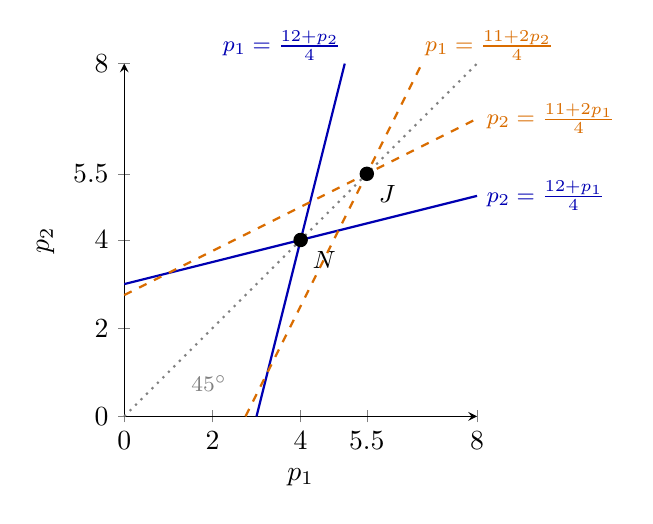
\begin{tikzpicture}
\begin{axis}[
  width=0.5\linewidth, height=0.5\linewidth,
  xmin=0, xmax=8, ymin=0, ymax=8,
  xlabel={$p_1$}, ylabel={$p_2$},
  xtick={0,2,4,5.5,8}, ytick={0,2,4,5.5,8},
  axis lines=left, every axis plot/.append style={thick},
  clip=false]
  \addplot[domain=0:8, samples=2, dotted, gray] {x};
  \addplot[blue!70!black, domain=0:8, samples=2, variable=t] ({(12 + t)/4}, {t});
  \addplot[blue!70!black, domain=0:8, samples=2] {(12 + x)/4};
  \addplot[orange!85!black, dashed, domain=0:8, samples=2, variable=t] ({(11 + 2*t)/4}, {t});
  \addplot[orange!85!black, dashed, domain=0:8, samples=2] {(11 + 2*x)/4};
  \addplot[only marks, mark=*, mark size=2.2pt, black] coordinates {(4,4) (5.5,5.5)};
  \node[anchor=north west, font=\small] at (axis cs:4.05,3.95) {$N$};
  \node[anchor=north west, font=\small] at (axis cs:5.55,5.45) {$J$};
  \node[blue!70!black, anchor=south east, font=\footnotesize, inner sep=1pt] at (axis cs:5.0,8.0) {$p_1 = \frac{12 + p_2}{4}$};
  \node[orange!85!black, anchor=south west, font=\footnotesize, inner sep=1pt] at (axis cs:6.75,8.0) {$p_1 = \frac{11 + 2p_2}{4}$};
  \node[blue!70!black, anchor=west, font=\footnotesize] at (axis cs:8.0,5.0) {$p_2 = \frac{12 + p_1}{4}$};
  \node[orange!85!black, anchor=west, font=\footnotesize] at (axis cs:8.0,6.75) {$p_2 = \frac{11 + 2p_1}{4}$};
  \node[gray, anchor=north west, font=\footnotesize] at (axis cs:1.3,1.15) {$45^\circ$};
\end{axis}
\end{tikzpicture}
\caption{Linear duopoly of \cref{ex:04-linear-duopoly} with $a = 10$, $b = 2$, $d = 1$ and $c = 1$. Solid lines are
the best responses of separate owners, which cross at $N = (4, 4)$. Dashed lines are the first-order loci of a
single owner of both products, each giving the optimal price of one product for a fixed price of the other. They
cross at $J = (5.5, 5.5)$. The dashed loci are not best responses of independent firms. Their slope equals the
diversion ratio $D = \frac{1}{2}$, twice the slope of the separate best responses, because the joint owner
recaptures half of the sales that each product loses.}
\label{fig:04-br-merger}
\end{figure}

\subsection{Worked example: logit demand}\label{sec:04-bertrand-logit}

The logit model gives closed forms for every object in \cref{sec:04-bertrand-matrix}. \Cref{ch:discrete,ch:logit}
derive it from random utility. Here we take the market shares as given. Let market size be one, so quantities
equal shares. Mean utility is $\delta_j = x_j\beta - \alpha p_j + \xi_j$, with observed characteristics $x_j$,
unobserved quality $\xi_j$ and price coefficient $\alpha > 0$. With the mean utility of the outside good
normalized to zero, shares are
\begin{equation*}
s_j(p) = \frac{e^{\delta_j}}{\Phi},
\qquad
s_0(p) = \frac{1}{\Phi},
\qquad
\Phi = 1 + \sum_{k = 1}^{J}e^{\delta_k}.
\end{equation*}
We call $\Phi$ the \emph{logit denominator}.

\casehead{Derivatives}
Changing $p_j$ affects only $e^{\delta_j}$, with $\frac{\partial e^{\delta_j}}{\partial p_j} = -\alpha e^{\delta_j}$,
so also $\frac{\partial\Phi}{\partial p_j} = -\alpha e^{\delta_j}$. The quotient rule gives the own derivative
\begin{align*}
\frac{\partial s_j}{\partial p_j}
&= \frac{(-\alpha e^{\delta_j})\,\Phi - e^{\delta_j}\,(-\alpha e^{\delta_j})}{\Phi^2} \\
&= -\alpha\frac{e^{\delta_j}}{\Phi}\Big(1 - \frac{e^{\delta_j}}{\Phi}\Big)
= -\alpha s_j(1 - s_j).
\end{align*}
For $k \ne j$ the numerator $e^{\delta_k}$ does not depend on $p_j$, so
$\frac{\partial s_k}{\partial p_j} = -\frac{e^{\delta_k}(-\alpha e^{\delta_j})}{\Phi^2} = \alpha s_js_k$. The same
step applies to $s_0 = \frac{1}{\Phi}$. Collecting,
\begin{equation}\label{eq:04-logit-derivs}
\frac{\partial s_j}{\partial p_j} = -\alpha s_j(1 - s_j),
\qquad
\frac{\partial s_k}{\partial p_j} = \alpha s_js_k \quad (k \ne j,\ k \ge 1),
\qquad
\frac{\partial s_0}{\partial p_j} = \alpha s_0s_j.
\end{equation}
These derivatives sum to zero over $k = 0, \dots, J$, as they must. Since $\frac{\partial s_0}{\partial p_j} > 0$,
\cref{prop:04-markup-positive} applies at every price vector. The own and cross elasticities are
\begin{equation*}
\varepsilon_j = \alpha p_j(1 - s_j),
\qquad
\varepsilon_{kj} = \frac{\partial s_k}{\partial p_j}\frac{p_j}{s_k} = \alpha p_js_j \quad \text{for every } k \ne j.
\end{equation*}
A change in $p_j$ moves every other product's share by the same percentage. This is the \emph{independence of
irrelevant alternatives} (IIA), whose consequences \cref{ch:logit} discusses.

\begin{proposition}[Logit markups]\label{prop:04-logit-markup}
Under logit demand with constant marginal costs, every solution of the first-order conditions
\eqref{eq:04-foc-scalar} gives all products of firm $f$ the same markup,
\begin{equation*}
p_j - mc_j = m_f = \frac{1}{\alpha(1 - S_f)}
\quad \text{for all } j \in \mathcal{J}_f,
\qquad
S_f = \sum_{k \in \mathcal{J}_f}s_k.
\end{equation*}
A single-product firm sets $p_j - mc_j = \frac{1}{\alpha(1 - s_j)}$.
\end{proposition}

\begin{proof}
Write the first-order condition for $j \in \mathcal{J}_f$ in shares, $s_j + \sum_{k \in \mathcal{J}_f}m_k\frac{\partial s_k}{\partial p_j} = 0$,
and substitute \eqref{eq:04-logit-derivs}:
\begin{equation*}
s_j - \alpha s_j(1 - s_j)m_j + \sum_{k \in \mathcal{J}_f\setminus\{j\}}\alpha s_js_km_k = 0.
\end{equation*}
Split the second term as $-\alpha s_jm_j + \alpha s_js_jm_j$ and merge $\alpha s_js_jm_j$ into the sum:
\begin{equation*}
s_j - \alpha s_jm_j + \alpha s_j\sum_{k \in \mathcal{J}_f}s_km_k = 0.
\end{equation*}
Divide by $\alpha s_j > 0$:
\begin{equation*}
m_j = \frac{1}{\alpha} + \sum_{k \in \mathcal{J}_f}s_km_k.
\end{equation*}
The right side is the same for every $j \in \mathcal{J}_f$, so all of the firm's products share one markup $m_f$.
Substituting $m_k = m_f$ gives $m_f = \frac{1}{\alpha} + S_fm_f$. Since $S_f \le 1 - s_0 < 1$, we can solve:
$m_f = \frac{1}{\alpha(1 - S_f)}$. A single-product firm has $S_f = s_j$.
\end{proof}

The proposition characterizes markups without giving them in closed form, because $S_f$ depends on prices. It
still has several sharp implications. Markups are bounded below by $\frac{1}{\alpha}$, whatever the number of
competitors. They depend on the firm only through its combined share. Product quality and cost affect markups
only by changing shares. Within a firm, dollar markups are equal, so a firm's high-cost products carry lower
percentage margins, $\frac{m_f}{p_j} = \frac{1}{\alpha p_j(1 - S_f)}$. Finally, a firm with a large combined share
sets high markups on all its products, including those with tiny shares.

As an illustration, suppose one firm owns products 1 and 2 with shares $s_1$ and $s_2$. It sets the markup
$\frac{1}{\alpha(1 - s_1 - s_2)}$ on both. If the products had separate owners, their markups would be
$\frac{1}{\alpha(1 - s_1)}$ and $\frac{1}{\alpha(1 - s_2)}$. Joint ownership raises the markup of the smaller
product by more. Under logit, the diversion ratio from product $k$ to product $j$ is $\frac{s_j}{1 - s_k}$
(\cref{sec:04-diversion-systems}). Diversion from the small product to the large one is therefore the larger of the
two, so joint ownership recaptures a larger fraction of the small product's lost sales.

\casehead{The best response in closed form}
For a single-product firm the first-order condition $\alpha m_j(1 - s_j) = 1$ is implicit, because $s_j$ depends
on $p_j$. It can nevertheless be solved explicitly. Define the mean utility of product $j$ at marginal-cost
pricing and the logit denominator without product $j$,
\begin{equation*}
v_j = x_j\beta + \xi_j - \alpha\,mc_j,
\qquad
\Phi_{-j} = 1 + \sum_{l \ne j}e^{\delta_l}.
\end{equation*}
Then $\delta_j = v_j - \alpha m_j$, and $\Phi_{-j}$ depends only on rivals' prices. The share and its complement
are
\begin{equation*}
s_j = \frac{e^{\delta_j}}{\Phi_{-j} + e^{\delta_j}},
\qquad
1 - s_j = \frac{\Phi_{-j}}{\Phi_{-j} + e^{\delta_j}}.
\end{equation*}
Substitute the complement into the first-order condition and multiply by $\Phi_{-j} + e^{\delta_j}$:
\begin{align*}
\alpha m_j\Phi_{-j} &= \Phi_{-j} + e^{\delta_j} \\
(\alpha m_j - 1)\Phi_{-j} &= e^{v_j - \alpha m_j}.
\end{align*}
Multiply both sides by $\frac{e^{\alpha m_j - 1}}{\Phi_{-j}}$:
\begin{equation*}
(\alpha m_j - 1)\,e^{\alpha m_j - 1} = \frac{e^{v_j - 1}}{\Phi_{-j}}.
\end{equation*}
The \emph{Lambert W function} $W(z)$ solves $W(z)e^{W(z)} = z$ \citep{CorlessEtAl1996}. For $z > 0$ the equation
$ye^y = z$ has exactly one real root, which is positive. Indeed $ye^y \le 0$ for $y \le 0$, while $ye^y$ rises
strictly from 0 to infinity on $y > 0$. Setting $y = \alpha m_j - 1$ gives the best response
\begin{equation}\label{eq:04-logit-br}
BR_j(p_{-j}) = mc_j + \frac{1}{\alpha}\Big[1 + W\Big(\frac{e^{v_j - 1}}{\Phi_{-j}}\Big)\Big].
\end{equation}
The formula shows three properties at a glance. The best-response markup exceeds $\frac{1}{\alpha}$ because
$W(z) > 0$. It rises with the product's quality net of cost, $v_j$. And it rises with every rival price, because
a higher $p_l$ lowers $\Phi_{-j}$ and $W$ is increasing. Logit prices are strategic complements.

The stationary point in \eqref{eq:04-logit-br} is the global maximizer of $\pi_j = m_js_j$. The derivative of
profit factors as
\begin{equation*}
\frac{\partial\pi_j}{\partial p_j} = s_j + m_j\frac{\partial s_j}{\partial p_j} = s_j\,g(p_j),
\qquad
g(p_j) = 1 - \alpha(p_j - mc_j)\big(1 - s_j(p_j)\big).
\end{equation*}
If $p_j \le mc_j$, then $g(p_j) \ge 1$ and profit is increasing. If $p_j > mc_j$, both $\alpha(p_j - mc_j)$ and
$1 - s_j(p_j)$ are positive and strictly increasing in $p_j$, so $g$ is strictly decreasing. As
$p_j \to \infty$, $g(p_j) \to -\infty$. Hence $g$ crosses zero exactly once, from above. Profit rises before the
crossing and falls after it, so the crossing is the unique global maximizer.

The multi-product analogue follows the same steps. By \cref{prop:04-logit-markup}, a stationary point of firm
$f$'s problem has a common markup $m_f$, so $e^{\delta_k} = e^{v_k - \alpha m_f}$ for $k \in \mathcal{J}_f$. Let
$E_f = \sum_{k \in \mathcal{J}_f}e^{v_k}$ and $\Phi_{-f} = 1 + \sum_{l \notin \mathcal{J}_f}e^{\delta_l}$. The
firm's combined share is
\begin{equation*}
S_f = \frac{E_fe^{-\alpha m_f}}{\Phi_{-f} + E_fe^{-\alpha m_f}}.
\end{equation*}
Repeating the algebra above with $E_f$ in place of $e^{v_j}$ and $S_f$ in place of $s_j$ gives
\begin{equation}\label{eq:04-logit-br-multi}
m_f^{BR}(p_{-\mathcal{J}_f}) = \frac{1}{\alpha}\Big[1 + W\Big(\frac{E_fe^{-1}}{\Phi_{-f}}\Big)\Big],
\qquad
p_k = mc_k + m_f^{BR} \ \text{ for } k \in \mathcal{J}_f.
\end{equation}
Showing that this stationary point is the firm's global optimum takes one more step. The firm's problem reduces to
the choice of a common markup, and the single-crossing argument then applies to $S_f$ in place of $s_j$. Steps 1
and 2 of the proof of \cref{thm:04-logit-unique} give the details, and \cref{sec:04-exercises} asks for the
algebra behind \eqref{eq:04-logit-br-multi}.

\subsection{A numerical illustration: 25 logit products}\label{sec:04-bertrand-logit25}

We now compute equilibria in a simulated market. The market reappears in \cref{sec:04-existence}, where we check
uniqueness, and as a worked problem in \cref{app:problems}.

\begin{example}[A 25-product logit market]\label{ex:04-logit25}
There are $J = 25$ products and market size one. Each product has three observed characteristics: a constant, a
continuous characteristic and a binary one, $x_j = (1, x_{j2}, x_{j3})$. It also has unobserved quality $\xi_j$ and
a cost shock $\omega_j$. Demand is logit with $\beta = (0.1, 0.25, 0.1)$ and $\alpha = 2$. Marginal cost is
$mc_j = x_j\gamma + \omega_j$ with $\gamma = (0.2, 0.25, 0.3)$, and it ranges from 0.164 to 1.236. All primitives
are common knowledge, and firms set prices simultaneously. We compare two ownership structures.
\begin{itemize}
  \item[(S)] Every product has its own owner, so $\Omega = I_{25}$.
  \item[(M)] Five owners, labeled 0 to 4, hold 3, 3, 6, 6 and 7 products.
\end{itemize}
Products are numbered 0 to 24 and owners 0 to 4, as in the data set of \cref{app:problems}. Here the label 0 names
an inside product, and $s_0$ still denotes the share of the outside good.
In (S) the first-order conditions are $s_j + (p_j - mc_j)\frac{\partial s_j}{\partial p_j} = 0$ for all $j$. In
(M) they are $s + (\Omega \odot \Delta^{s\top})(p - mc) = 0$ with the owners' $\Omega$. A Nash equilibrium is a
price vector at which no owner can raise its profit by changing its own prices, which is a fixed point of the
best-response map.
\end{example}

\begin{remark}[Computing the equilibrium]\label{rem:04-logit25-algorithm}
We compute each equilibrium by best-response iteration.
\begin{enumerate}
  \item Start from $p^{(0)} = mc + \frac{1}{\alpha}$, the lower bound on logit markups.
  \item Given $p^{(n)}$, compute for every owner $f$ the quantities $E_f$ and $\Phi_{-f}(p^{(n)})$, the markup
  $m_f$ from \eqref{eq:04-logit-br-multi}, and set $p^{(n+1)}_k = mc_k + m_f$ for $k \in \mathcal{J}_f$. In (S)
  every owner has one product and the step is \eqref{eq:04-logit-br}.
  \item Stop when $\|p^{(n+1)} - p^{(n)}\|_\infty < 10^{-12}$. Otherwise return to step 2.
  \item Check that the first-order residuals $s + (\Omega \odot \Delta^{s\top})(p - mc)$ vanish and that each
  owner's markup equals $\frac{1}{\alpha(1 - S_f)}$.
\end{enumerate}
The iteration converges in 10 steps in (S) and 15 steps in (M). As a cross-check we also iterate on the markup
equation, $p \leftarrow mc - (\Omega \odot \Delta^s(p)^\top)^{-1}s(p)$, which converges in 14 and 30 steps to the
same prices (largest difference $1.4 \times 10^{-13}$). The largest first-order residual is below
$2 \times 10^{-14}$. Markup iteration is simple and fast here, but it is not guaranteed to converge in general
(\cref{sec:04-counterfactuals}).
\end{remark}

\Cref{tab:04-logit25} reports the results by owner, and \cref{fig:04-logit25-markups} shows every product's
markup. In (S) each product is priced by a separate firm, and the owner rows aggregate those products for
comparison with (M). Consumer surplus is measured by $\frac{1}{\alpha}\ln\Phi$, the logit expected maximum utility
in money units (\cref{ch:logit}). We measure it relative to a market in which only the outside good is available,
where $\Phi = 1$. Its level is then the surplus that consumers get from the inside goods, so percentage changes are
meaningful.

\begin{table}[htbp]
\centering
\caption{Bertrand-Nash equilibrium in the 25-product logit market}
\label{tab:04-logit25}
\footnotesize
\begin{tabular}{@{}lccccccc@{}}
\toprule
 & & \multicolumn{2}{c}{Combined share $S_f$ (\%)} & \multicolumn{2}{c}{Markup} & \multicolumn{2}{c}{Profit $\times 100$} \\
\cmidrule(lr){3-4}\cmidrule(lr){5-6}\cmidrule(l){7-8}
Owner & Products & (S) & (M) & (S) & (M) & (S) & (M) \\
\midrule
\multicolumn{8}{@{}l}{\textit{Panel A. Owners}} \\
0 & 3 & 18.32 & 18.87 & 0.552 & 0.616 & 10.112 & 11.632 \\
1 & 3 & 4.12 & 4.67 & 0.508 & 0.524 & 2.094 & 2.449 \\
2 & 6 & 13.27 & 13.68 & 0.516 & 0.579 & 6.841 & 7.925 \\
3 & 6 & 22.62 & 21.40 & 0.529 & 0.636 & 11.971 & 13.616 \\
4 & 7 & 28.00 & 25.36 & 0.541 & 0.670 & 15.145 & 16.989 \\
\midrule
\multicolumn{8}{@{}l}{\textit{Panel B. Market}} \\
\multicolumn{4}{@{}l}{Outside share $s_0$} & 0.1367 & 0.1601 & & \\
\multicolumn{4}{@{}l}{Logit denominator $\Phi^* = \frac{1}{s_0}$} & 7.314 & 6.246 & & \\
\multicolumn{4}{@{}l}{Consumer surplus $\frac{1}{\alpha}\ln\Phi^*$} & 0.9949 & 0.9159 & & \\
\multicolumn{4}{@{}l}{Total profit} & 0.4616 & 0.5261 & & \\
\multicolumn{4}{@{}l}{Total surplus (consumer surplus plus profit)} & 1.4565 & 1.4421 & & \\
\multicolumn{4}{@{}l}{Share-weighted mean price} & 1.2599 & 1.3553 & & \\
\bottomrule
\end{tabular}

\vspace{3pt}
\begin{minipage}{0.97\textwidth}
\footnotesize Notes: (S) single-product firms, (M) five multi-product owners. In column (S) the owner rows add
up shares and profits of products that are priced independently, and the markup is the share-weighted mean
over the owner's products. In column (M) every product of an owner carries the same markup
$\frac{1}{\alpha(1 - S_f)}$. Market size is one, so profits and consumer surplus are per consumer. Computed with
\texttt{figures/ch04/src/logit25.py}.
\end{minipage}
\end{table}

\begin{figure}[htbp]
\centering
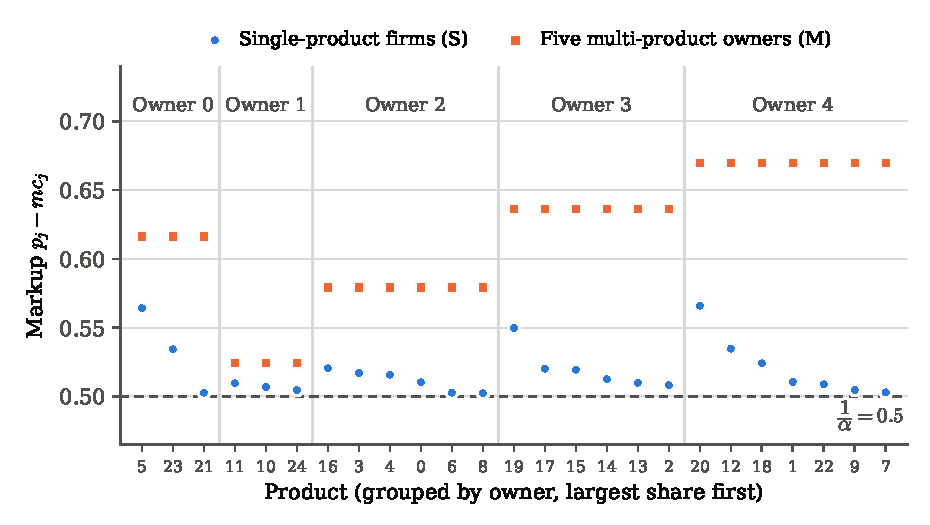
\includegraphics[width=\linewidth]{figures/ch04/logit25_markups.pdf}
\caption{Equilibrium markups $p_j - mc_j$ in the 25-product logit market. Circles show single-product firms (S),
squares show the five multi-product owners (M). Products are grouped by owner and sorted by share. Under (S)
markups are close to the floor $\frac{1}{\alpha} = 0.5$ and rise with the product's own share. Under (M) all
products of an owner share the markup $\frac{1}{\alpha(1 - S_f)}$.}
\label{fig:04-logit25-markups}
\end{figure}

The results illustrate the theory of this section in five ways.

First, single-product markups lie between 0.502 and 0.566, close to the floor $\frac{1}{\alpha} = 0.5$. Each
product has a small share, so $\frac{1}{\alpha(1 - s_j)}$ barely exceeds $\frac{1}{\alpha}$. The largest markups
belong to the products with the largest shares, products 20 and 5, whose shares are 11.7 and 11.4 percent.

Second, multi-product ownership raises every owner's markup to $\frac{1}{\alpha(1 - S_f)}$. The common markups range
from 0.524 for owner 1, whose products have a combined share near 5 percent, to 0.670 for owner 4, whose
combined share is about 25 percent. A product with a share of half a percent, such as product 7, carries the same
markup as owner 4's largest product. Its price rises the most, by 0.167.

Third, every price rises, by amounts from 0.015 (product 11) to 0.167 (product 7). Two forces combine. Each owner
internalizes cannibalization among its own products, and prices are strategic complements, so each owner also
responds to the higher prices of the others. To isolate the second force, we recomputed the equilibrium with only
owner 4 consolidating its seven products and all other products independent. Owner 4's prices rise by 0.089 to
0.152, and rivals' prices rise by 0.0001 to 0.0040 through strategic complementarity. In that exercise rivals'
combined profit rises from 0.3102 to 0.3296, while owner 4's profit rises only from 0.1515 to 0.1553. The
non-consolidating firms gain more than the firm that consolidates.

Fourth, shares move away from the owners that raise prices most. The two largest owners lose share, owner 4
from 28.00 to 25.36 percent and owner 3 from 22.62 to 21.40 percent. The three smaller owners gain. Fifteen of the
25 products lose share, and the outside share rises from 0.137 to 0.160.

Fifth, total profit rises by about 14 percent, from 0.4616 to 0.5261. Consumer surplus falls by 0.079, or 7.9
percent, and total surplus falls from 1.4565 to 1.4421. In equilibrium the logit denominator equals
$\frac{1}{s_0}$, which falls from 7.314 to 6.246. \Cref{sec:04-existence} shows that this aggregate pins down
the whole equilibrium. It uses this to prove that the logit equilibrium is unique for any ownership structure
\citep{KonovalovSandor2010,NockeSchutz2018}, and \cref{ex:04-logit25-unique} confirms numerically that the two
equilibria in \cref{tab:04-logit25} are the only ones.

\section{Diversion ratios}\label{sec:04-diversion}

The pricing rule of \cref{sec:04-bertrand} depends on own-price and cross-price derivatives of demand.
Elasticities summarize these derivatives product by product. Diversion ratios summarize them pair by pair:
they record where the customers of a product go when its price rises. This makes them the natural language
for three questions that recur in this book. Which products compete most closely? How does a multi-product
firm price products that cannibalize one another? Which mergers create an incentive to raise prices? This
section defines diversion ratios, rewrites the first-order condition in terms of them, computes them in the
standard demand systems, and lists what they cannot tell us.

\subsection{Definitions and basic properties}\label{sec:04-diversion-def}

We keep the environment of \cref{ass:04-bertrand}. To lighten the notation we write
\[
  \partial_k q_j \equiv \frac{\partial q_j(p)}{\partial p_k}
\]
for the derivative of the demand for product $j$ with respect to the price of product $k$. In this notation
the $(j,k)$ element of $\Delta$ is $\partial_k q_j$. The \emph{cross-price derivative} $\partial_j q_k$ is the
change in the sales of product $k$ when the price of product $j$ rises by one dollar. The \emph{cross-price
elasticity} is $\varepsilon_{kj} = \frac{\partial q_k}{\partial p_j}\frac{p_j}{q_k}$, and the own-price
elasticity is the positive number $\varepsilon_j = -\frac{\partial q_j}{\partial p_j}\frac{p_j}{q_j}$.

\begin{definition}[Diversion ratio]\label{def:04-diversion}
For two inside products $j \neq k$, the \emph{diversion ratio} from $j$ to $k$ is
\begin{equation}\label{eq:04-diversion-def}
  D_{jk} = -\frac{\partial_j q_k}{\partial_j q_j}.
\end{equation}
The \emph{diversion ratio to the outside good} is $D_{j0} = 1 - \sum_{k \ge 1, k \neq j} D_{jk}$, and the
\emph{aggregate diversion ratio} of product $j$ is $\sum_{k \ge 1, k \neq j} D_{jk} = 1 - D_{j0}$.
\end{definition}

The numerator and the denominator of \eqref{eq:04-diversion-def} refer to the same experiment, a small
increase $\dd p_j$ in the price of product $j$ with all other prices fixed. Product $j$ loses
$-\partial_j q_j \, \dd p_j$ units of sales. Product $k$ gains $\partial_j q_k\, \dd p_j$ units. The diversion
ratio is the fraction of the lost units that product $k$ recaptures. Read in reverse, it is the number of
units of $k$ that are lost when $p_j$ falls by enough to sell one more unit of $j$. The first index always
names the product whose price changes. In general $D_{jk} \neq D_{kj}$.

\begin{proposition}[Adding up]\label{prop:04-diversion-adding}
Suppose that each of $M$ consumers buys exactly one unit of one of the options $0, 1, \dots, J$, so that
$\sum_{k=0}^J q_k(p) = M$ for every price vector $p$. Then for every inside product $j$,
\begin{equation}\label{eq:04-diversion-adding}
  \sum_{k \ge 1,\, k \neq j} D_{jk} + D_{j0} = 1, \qquad\text{with}\qquad D_{j0} = -\frac{\partial_j q_0}{\partial_j q_j}.
\end{equation}
If all products, including the outside good, are gross substitutes, every diversion ratio lies in $[0,1]$.
\end{proposition}

\begin{proof}
Differentiate the identity $\sum_{k=0}^J q_k(p) = M$ with respect to $p_j$. The right side does not depend
on prices, so
\[
  \partial_j q_j + \sum_{k \ge 1,\, k \neq j}\partial_j q_k + \partial_j q_0 = 0.
\]
Divide by $-\partial_j q_j > 0$:
\[
  -1 + \sum_{k \ge 1,\, k\neq j}\Bigl(-\frac{\partial_j q_k}{\partial_j q_j}\Bigr) + \Bigl(-\frac{\partial_j q_0}{\partial_j q_j}\Bigr) = 0.
\]
The terms in parentheses are $D_{jk}$ and $-\frac{\partial_j q_0}{\partial_j q_j}$, which gives
\eqref{eq:04-diversion-adding}. Under gross substitutes each term is nonnegative. Nonnegative numbers
that sum to one each lie in $[0,1]$.
\end{proof}

In unit-demand models the residual $D_{j0}$ in \cref{def:04-diversion} is the share of lost customers who
stop buying any inside product. A large $D_{j0}$ then means that the products in the group constrain one
another little. This is why the aggregate diversion ratio appears in market definition (\cref{ch:mergers}).
Some demand systems have no explicit outside option, such as the linear and CES systems of
\cref{sec:04-repcons}. Their quantities need not add up in units, so $D_{j0}$ is only the residual of
\cref{def:04-diversion}. It changes when we rescale the units of one product, and in CES it can be negative.
Reading it as the fraction of $j$'s lost units that the group does not recapture requires units that are
comparable across products.

Diversion ratios and elasticities carry the same information, arranged differently. Write each derivative
in terms of an elasticity:
\[
  \partial_j q_k = \varepsilon_{kj}\frac{q_k}{p_j}, \qquad \partial_j q_j = -\varepsilon_j\frac{q_j}{p_j}.
\]
Substituting into \eqref{eq:04-diversion-def}, the price $p_j$ cancels and
\begin{equation}\label{eq:04-diversion-elast}
  D_{jk} = \frac{\varepsilon_{kj}}{\varepsilon_j}\,\frac{q_k}{q_j}.
\end{equation}
A large cross elasticity does not imply a large diversion ratio. If product $k$ is small, a large percentage
gain for $k$ is a small number of units. Conversely, a large product can capture many of $j$'s customers even
when its own percentage gain is modest.

\casehead{Measurement}
Diversion ratios can be computed from an estimated demand system (\cref{ch:logit,ch:blp}). They can also be
measured more directly, which is a large part of their appeal to antitrust agencies. Firms often track whom
they lose business to, and surveys can ask buyers of $j$ what they would have bought instead
\citep[p.~16]{FarrellShapiro2010}. Natural experiments that remove a product, such as stock-outs, recalls and
exits, reveal where its customers go. In bidding markets the diversion ratio from $j$ to $k$ can be read as
the probability that $k$ is the runner-up when $j$ wins \citep[p.~16]{FarrellShapiro2010}.

These sources do not all measure the same object. \citet{ConlonMortimer2021} view a diversion ratio as a
treatment effect and stress that the size of the price change matters. Second-choice data describe what
happens when product $j$ disappears, which is a price increase to infinity. The pricing incentive in
\eqref{eq:04-foc-diversion} below involves a marginal price change. A mixture of logits shows the
difference. Let consumer types $i$ have distribution $F$, price coefficient $\alpha_i$ and logit choice
probabilities $s_{ij}$, so that $s_j = \int s_{ij}\,\dd F(i)$. Using \eqref{eq:04-logit-derivs} type by type,
the marginal diversion ratio is
\begin{equation}\label{eq:04-diversion-marginal}
  D_{jk} = \frac{\int \alpha_i s_{ij}s_{ik}\,\dd F(i)}{\int \alpha_i s_{ij}(1 - s_{ij})\,\dd F(i)}
         = \int \varpi_i\,\frac{s_{ik}}{1 - s_{ij}}\,\dd F(i),
  \qquad \varpi_i = \frac{\alpha_i s_{ij}(1 - s_{ij})}{\int \alpha_{i'} s_{i'j}(1 - s_{i'j})\,\dd F(i')}.
\end{equation}
When $j$ is removed, a type-$i$ buyer of $j$ moves to $k$ with probability
$\frac{e^{\delta_{ik}}}{\sum_{l \neq j}e^{\delta_{il}}} = \frac{s_{ik}}{1 - s_{ij}}$, where $\delta_{il}$ is the
mean utility of option $l$ for type $i$. Averaging over the buyers of $j$ gives the second-choice diversion
ratio
\begin{equation}\label{eq:04-diversion-secondchoice}
  D^{\mathrm{SC}}_{jk} = \int \tilde\varpi_i\,\frac{s_{ik}}{1 - s_{ij}}\,\dd F(i), \qquad \tilde\varpi_i = \frac{s_{ij}}{s_j}.
\end{equation}
Both are weighted averages of the same type-level ratios $\frac{s_{ik}}{1 - s_{ij}}$. The marginal ratio
weights types by $\alpha_i s_{ij}(1 - s_{ij})$, which is large for price-sensitive consumers near the margin
of buying $j$. The second-choice ratio weights all current buyers of $j$ equally. With one type both reduce
to the logit formula $\frac{s_k}{1 - s_j}$. With heterogeneous consumers they differ, and a survey answer
needs a model before it can be plugged into a pricing formula.

\subsection{The first-order condition in diversion form}\label{sec:04-diversion-foc}

The multi-product first-order condition \eqref{eq:04-foc-scalar} can be rewritten so that diversion ratios
appear explicitly. For firm $f$ and a product $j \in \mathcal{J}_f$ the condition reads
\[
  q_j + \sum_{k \in \mathcal{J}_f}(p_k - mc_k)\,\partial_j q_k = 0.
\]
We first split off the term $k = j$:
\[
  q_j + (p_j - mc_j)\,\partial_j q_j + \sum_{k \in \mathcal{J}_f\setminus\{j\}}(p_k - mc_k)\,\partial_j q_k = 0.
\]
Next we divide by $\partial_j q_j < 0$:
\[
  \frac{q_j}{\partial_j q_j} + (p_j - mc_j) + \sum_{k \in \mathcal{J}_f\setminus\{j\}}(p_k - mc_k)\frac{\partial_j q_k}{\partial_j q_j} = 0.
\]
Solving for $p_j$ gives
\[
  p_j = mc_j - \frac{q_j}{\partial_j q_j} - \sum_{k \in \mathcal{J}_f\setminus\{j\}}(p_k - mc_k)\frac{\partial_j q_k}{\partial_j q_j}.
\]
Finally, $-\frac{\partial_j q_k}{\partial_j q_j} = D_{jk}$ by \eqref{eq:04-diversion-def}, so
\begin{equation}\label{eq:04-foc-diversion}
  p_j = mc_j + \frac{q_j}{-\partial_j q_j} + \sum_{k \in \mathcal{J}_f\setminus\{j\}} D_{jk}\,(p_k - mc_k).
\end{equation}

The price of product $j$ has three parts. The first is marginal cost. The second is the markup a
single-product firm would charge, the reciprocal of the absolute semi-elasticity of $q_j$. The third is the
\emph{value of diverted sales}: each unit of $j$'s lost sales that moves to a sibling product $k$ earns the
firm the margin $p_k - mc_k$. This term is an opportunity cost of selling $j$, because every extra unit of $j$
cannibalizes $D_{jk}$ units of $k$. Define the \emph{effective marginal cost}
$\widetilde{mc}_j = mc_j + \sum_{k \in \mathcal{J}_f\setminus\{j\}}D_{jk}(p_k - mc_k)$. Then
\eqref{eq:04-foc-diversion} becomes $p_j - \widetilde{mc}_j = \frac{q_j}{-\partial_j q_j}$, and dividing by
$p_j$,
\[
  \frac{p_j - \widetilde{mc}_j}{p_j} = \frac{1}{\varepsilon_j}.
\]
A multi-product firm prices each product by the inverse elasticity rule, applied to an effective marginal cost
that includes the value of diverted sales. The 2010 US Horizontal Merger Guidelines use this phrase for the units
diverted to a product multiplied by that product's margin \citep[Section 6.1, p.~21]{USDOJFTC2010}. The term in
\eqref{eq:04-foc-diversion} is this value per unit of lost sales of $j$.

Stacking \eqref{eq:04-foc-diversion} over products gives a compact matrix version. Let
$m^{\mathrm{s}}_j = \frac{q_j}{-\partial_j q_j}$ be the single-product markup, with vector $m^{\mathrm{s}}$, let
$m = p - mc$, and let $\mathcal{D}$ be the $J \times J$ \emph{diversion matrix} with $\mathcal{D}_{jk} = D_{jk}$ for
$k \neq j$ and zeros on the diagonal. Since $\Omega_{jk} = 1$ exactly when $j$ and $k$ have the same owner,
\begin{equation}\label{eq:04-markup-diversion}
  m = m^{\mathrm{s}} + (\Omega \odot \mathcal{D})\,m, \qquad\text{so}\qquad m = (I - \Omega \odot \mathcal{D})^{-1} m^{\mathrm{s}}.
\end{equation}
This is the stacked first-order condition \eqref{eq:04-foc-matrix} with row $j$ divided by $-\partial_j q_j$, and its
solution coincides with the markup equation \eqref{eq:04-markup}.

\begin{remark}\label{rem:04-diversion-positive}
Equation \eqref{eq:04-markup-diversion} gives a short proof that markups are positive. Suppose that every
outside diversion ratio is positive, $D_{j0} > 0$. Row $j$ of $\Omega\odot\mathcal{D}$ has nonnegative
entries that sum to at most $\sum_{k \neq j}D_{jk} = 1 - D_{j0} < 1$. The sup-norm of
$\Omega\odot\mathcal{D}$ is therefore below one, and the Neumann series
$(I - \Omega\odot\mathcal{D})^{-1} = \sum_{n=0}^\infty(\Omega\odot\mathcal{D})^n$ converges to a matrix with
nonnegative entries and diagonal entries of at least one. Hence $m \ge m^{\mathrm{s}} > 0$ element by element. Every product of a
multi-product firm carries at least its single-product markup, in line with \cref{prop:04-markup-positive}.
\end{remark}

Two examples from \cref{sec:04-bertrand} show the formula at work. In the linear duopoly of
\cref{ex:04-linear-duopoly}, $\partial_1 q_1 = -b$ and $\partial_1 q_2 = d$, so $D_{12} = \frac{d}{b} \equiv D$.
For a joint owner, \eqref{eq:04-foc-diversion} reads $m_1 = \frac{q_1}{b} + D\,m_2$. At a symmetric
solution $m(1 - D) = \frac{q}{b}$ with $q = a - (b - d)(c + m)$. Multiplying by $b$ and using
$b(1 - D) = b - d$,
\[
  (b - d)\,m = a - (b - d)c - (b - d)m \quad\Longrightarrow\quad m^J = \frac{a - (b - d)c}{2(b - d)},
\]
the joint-owner markup found in \cref{ex:04-linear-duopoly}. In the multi-product logit model the
derivatives \eqref{eq:04-logit-derivs} give $D_{jk} = \frac{s_k}{1 - s_j}$ and
$m^{\mathrm{s}}_j = \frac{1}{\alpha(1 - s_j)}$. With the common markup $m_f$ of \cref{prop:04-logit-markup},
\eqref{eq:04-foc-diversion} becomes
\[
  m_f = \frac{1}{\alpha(1 - s_j)} + \frac{S_f - s_j}{1 - s_j}\,m_f
  \quad\Longrightarrow\quad m_f\,\frac{1 - S_f}{1 - s_j} = \frac{1}{\alpha(1 - s_j)}
  \quad\Longrightarrow\quad m_f = \frac{1}{\alpha(1 - S_f)},
\]
where $S_f = \sum_{k \in \mathcal{J}_f}s_k$. The firm's combined share enters because the recaptured
fraction $\frac{S_f - s_j}{1 - s_j}$ grows with the shares of the sibling products.

\subsection{Why diversion governs the unilateral effects of mergers}\label{sec:04-diversion-merger}

Equation \eqref{eq:04-foc-diversion} explains why diversion ratios dominate the analysis of
\emph{unilateral effects}. These are the price effects of a merger that arise because the merged firm
internalizes competition between its own products, with the conduct of rivals unchanged. A merger adds the
acquired products to $\mathcal{J}_f\setminus\{j\}$ and so adds terms $D_{jk}(p_k - mc_k)$ to the effective marginal
cost of product $j$. The size of these terms depends on how close the merging products are as substitutes. The
merging firms' shares of a predefined market play no direct role.

Consider two single-product Bertrand firms, $A$ selling product 1 and $B$ selling product 2, with constant
marginal costs. Before the merger, firm $A$'s first-order condition is
$q_1 + (p_1 - mc_1)\,\partial_1 q_1 = 0$. After the merger, one owner maximizes $\pi_1 + \pi_2$. Evaluated at
the pre-merger prices, the derivative of joint profit with respect to $p_1$ is
\[
  \frac{\partial(\pi_1 + \pi_2)}{\partial p_1}
  = \underbrace{q_1 + (p_1 - mc_1)\,\partial_1 q_1}_{=\,0 \text{ before the merger}} + (p_2 - mc_2)\,\partial_1 q_2
  = (p_2 - mc_2)\,\partial_1 q_2 > 0.
\]
The merged firm wants to raise $p_1$. Dividing by $-\partial_1 q_1 > 0$ measures this incentive per unit of
product 1's lost sales. The result, $D_{12}(p_2 - mc_2)$, is the increase in the effective marginal cost of
product 1. \citet[p.~9]{FarrellShapiro2010} interpret it as a ``first-round tax'' that the merged firm's
headquarters would levy on division $A$ to make it internalize the sales it takes from division $B$.

A merger can also lower marginal costs. Let $E_1$ be the proportional reduction in the marginal cost of product
1, so that the merger saves $E_1 mc_1$ per unit. The symbol $E_1$ is unrelated to the logit aggregate $E_f$ of
\cref{sec:04-bertrand-logit}. The \emph{upward pricing pressure} (UPP) on product 1 is
\begin{equation}\label{eq:04-upp}
  \mathit{UPP}_1 = D_{12}(p_2 - mc_2) - E_1\,mc_1,
\end{equation}
evaluated at pre-merger prices and margins. \citet[p.~12, inequality (1)]{FarrellShapiro2010} propose to
presume harm when $\mathit{UPP}_1 > 0$. In the symmetric case, with equal prices $p$, costs $mc$, diversion
ratios $D$ and efficiencies $E$, the condition divides through by $p - mc$ to give
\[
  D > E\,\frac{mc}{p - mc}.
\]
This is their inequality (2), which they state in terms of the relative margin $\frac{p - mc}{p}$. They use $E = 0.1$ as an illustrative default
\citep[p.~10]{FarrellShapiro2010}. With a Lerner index of $\frac{1}{3}$ we have $\frac{mc}{p - mc} = 2$, and the
merger is flagged when $D > 0.2$.

Condition \eqref{eq:04-upp} credits an efficiency to product 1 only. Suppose that the merger also lowers the
marginal cost of product 2 by the fraction $E_2$. Each unit diverted to product 2 then earns the margin
$p_2 - (1 - E_2)mc_2 = (p_2 - mc_2) + E_2\,mc_2$, which is larger even at unchanged prices. At pre-merger prices
the derivative of joint profit with respect to $p_1$, divided by $-\partial_1 q_1$, becomes
\[
  D_{12}\big[(p_2 - mc_2) + E_2\,mc_2\big] - E_1\,mc_1.
\]
In the symmetric case with $E_1 = E_2 = E$ it is positive exactly when $D(p - mc) > (1 - D)E\,mc$, that is, when
$\frac{D}{1 - D} > E\frac{mc}{p - mc}$ \citep[p.~14, inequality (4)]{FarrellShapiro2010}. At equality the
pre-merger prices satisfy both post-merger first-order conditions. The common efficiency $E$ then equals the
compensating marginal-cost reduction of \citet{Werden1996}, which leaves both prices unchanged. Farrell and
Shapiro obtain the general version, their inequality (3), by solving these two markup equations simultaneously.
With the same numbers the condition reads $\frac{D}{1 - D} > 0.2$, so the threshold falls to
$D > \frac{1}{6} \approx 0.167$. Their footnote 35 reports both thresholds, 20 and 16.7 percent. It also notes
that the symmetric condition is equivalent to equation (6) of \citet{Werden1996}. The responses of the two prices
to each other after the merger are a separate feedback. When $p_2$ rises, the margin on diverted sales grows
further and adds to the pricing pressure on product 1 \citep[p.~13]{FarrellShapiro2010}. This feedback changes
the size of the price increase but leaves the threshold unchanged. At the threshold the pre-merger prices already
satisfy both post-merger first-order conditions, so no price moves.

The \emph{gross upward pricing pressure index} (GUPPI) scales the cannibalization term by the price of the product
under study:
\begin{equation}\label{eq:04-guppi}
  \mathit{GUPPI}_1 = \frac{D_{12}(p_2 - mc_2)}{p_1} = D_{12}\,\frac{p_2 - mc_2}{p_2}\,\frac{p_2}{p_1}.
\end{equation}
For example, $D_{12} = 0.2$, a margin of 40 percent on product 2 and equal prices give
\[
  \mathit{GUPPI}_1 = 0.2 \times 0.4 \times 1 = 0.08.
\]
The merger raises the effective marginal cost of product 1 by 8 percent of its price. UPP and GUPPI need
only diversion ratios and margins, and no full demand system. \citet[p.~12, Proposition 1]{FarrellShapiro2010}
show that net upward pricing pressure on both products, with no more than the default efficiencies, implies
that both prices rise. A full merger simulation instead solves the post-merger first-order conditions
$q + (\Omega^{post}\odot\Delta^\top)(p - mc) = 0$ with recovered marginal costs (\cref{sec:04-counterfactuals}).
The derivation with efficiencies, the role of pass-through, the GUPPI thresholds used in practice and
applications are in \cref{ch:mergers}.

\begin{example}[From UPP to price effects in the linear duopoly]\label{ex:04-upp-linear}
The linear duopoly of \cref{ex:04-linear-duopoly} shows how a diversion-based pricing pressure translates into a
price change. Before the merger each markup is $m^N = \frac{a - (b - d)c}{2b - d}$. After it, each markup is
$m^J$, and the ratio is
\[
  \frac{m^J}{m^N} = \frac{2b - d}{2(b - d)} = \frac{2 - D}{2 - 2D}, \qquad D = \frac{d}{b}.
\]
The ratio equals 1.056, 1.167, 1.5 and 2.5 for $D = 0.1$, $0.25$, $0.5$ and $0.75$. In levels,
\[
  m^J - m^N = m^N\Bigl(\frac{2 - D}{2 - 2D} - 1\Bigr) = \frac{D\,m^N}{2(1 - D)}.
\]
Without efficiencies the pre-merger UPP on each product is $D\,m^N$, so the price change is
$\frac{1}{2(1 - D)}$ times the UPP. The factor arises in three rounds. Holding the rival's price fixed, a firm
facing linear demand passes through one half of a cost increase, since its best response
$\frac{a + b(c + t) + d p_k}{2b}$ rises by $\frac{t}{2}$ for a cost increase $t$. If both products bear the
tax $t$ and both prices adjust, the symmetric equilibrium price $\frac{a + b(c + t)}{2b - d}$ rises by
$\frac{t}{2 - D}$. If the tax is then recomputed at the new margins, $t = D(m^N + \Delta p)$. Solving
$\Delta p\,(2 - D) = D(m^N + \Delta p)$ gives $\Delta p = \frac{D\,m^N}{2 - 2D}$, the full effect. The three
rounds follow the iterative procedure of \citet[p.~9]{FarrellShapiro2010}. We impose the internal taxes, let the
oligopoly re-equilibrate, re-calculate the taxes at the new prices and outputs, and repeat these steps until
convergence. Their footnote 24 adds that with strategic complements each round raises prices, so with constant
costs and diversion ratios the taxes rise from round to round. With $a = 10$, $b = 2$,
$d = 1$ and $c = 1$, we have $m^N = 3$, $D = \frac{1}{2}$ and $\mathit{UPP} = 1.5$. The price rises from 4 to
5.5, by exactly the UPP, because $\frac{1}{2(1 - D)} = 1$ when $D = \frac{1}{2}$.
\end{example}

\subsection{Diversion in standard demand systems}\label{sec:04-diversion-systems}

Each demand system used in practice implies a pattern of diversion. Often the pattern is imposed by the
functional form, which is worth knowing before a system is used to evaluate mergers.

\casehead{Logit}
With logit shares, \eqref{eq:04-logit-derivs} gives $\partial_j s_j = -\alpha s_j(1 - s_j)$,
$\partial_j s_k = \alpha s_j s_k$ and $\partial_j s_0 = \alpha s_j s_0$. Hence
\begin{equation}\label{eq:04-diversion-logit}
  D_{jk} = \frac{\alpha s_j s_k}{\alpha s_j(1 - s_j)} = \frac{s_k}{1 - s_j}, \qquad D_{j0} = \frac{s_0}{1 - s_j}.
\end{equation}
Customers who leave $j$ spread over the remaining options in proportion to their shares. A product similar to
$j$ and a product very different from it receive the same diversion if they have the same share. This is the
independence of irrelevant alternatives property (\cref{ch:logit}). It also means that a logit-based UPP adds
no information beyond shares and margins.

\casehead{CES}
Consider the CES system of \cref{sec:04-repcons} with elasticity of substitution $\sigma > 1$. This $\sigma$ is
unrelated to the nesting parameter. Demand is $q_j = \frac{p_j^{-\sigma}}{\sum_k p_k^{1-\sigma}}\,y$, with income $y$
and expenditure shares $s_j = \frac{p_jq_j}{y}$. The quantity diversion ratio is
\begin{equation}\label{eq:04-diversion-ces}
  D_{jk} = \frac{(\sigma - 1)\,p_j\,q_k}{y\,[\sigma - (\sigma - 1)s_j]} = \frac{(\sigma - 1)\,s_k}{\sigma - (\sigma - 1)s_j}\,\frac{p_j}{p_k},
\end{equation}
which \cref{prop:04-ces} derives from the CES elasticities. Diversion is proportional to the quantity $q_k$,
again with no role for similarity.

\casehead{Linear demand}
If $q = a + Ap$ for a vector $a$ and a $J \times J$ matrix $A$, then $\partial_j q_k = A_{kj}$ and
$D_{jk} = -\frac{A_{kj}}{A_{jj}}$. Diversion is constant, and in the symmetric duopoly it equals
$\frac{d}{b}$. A linear system can represent any pattern of diversion at one point, at the cost of $J^2$
price parameters (\cref{sec:04-spaces}).

\casehead{Nested logit}
Group the inside products into nests and let $\sigma^{\mathrm{NL}} \in [0,1)$ be the nesting parameter of
\cref{ch:logit}, written with a superscript in this section to avoid a clash with the CES elasticity. Let
$s_{j\mid g}$ be the share of product $j$ within its nest $g$ and $s_g$ the share of the nest. We use the form
of \citet{Berry1994}, and \cref{ch:logit} derives the share derivatives. With respect to $p_j$ they are
\[
  \partial_j s_j = -\frac{\alpha s_j\bigl[1 - \sigma^{\mathrm{NL}} s_{j\mid g} - (1 - \sigma^{\mathrm{NL}})s_j\bigr]}{1 - \sigma^{\mathrm{NL}}},
  \qquad
  \partial_j s_k = \frac{\alpha s_k\bigl[\sigma^{\mathrm{NL}} s_{j\mid g} + (1 - \sigma^{\mathrm{NL}})s_j\bigr]}{1 - \sigma^{\mathrm{NL}}}
\]
for $k$ in the nest of $j$, and $\partial_j s_k = \alpha s_k s_j$ for $k$ in another nest or $k = 0$. Taking ratios
and using $s_k = s_{k\mid g}s_g$ and $s_j = s_{j\mid g}s_g$,
\begin{equation}\label{eq:04-diversion-nl}
  D_{jk} =
  \begin{cases}
    \displaystyle\frac{s_{k\mid g}\bigl[\sigma^{\mathrm{NL}} + (1 - \sigma^{\mathrm{NL}})s_g\bigr]}{1 - \sigma^{\mathrm{NL}}s_{j\mid g} - (1 - \sigma^{\mathrm{NL}})s_j} & \text{if $k$ is in the nest of $j$,}\\[3ex]
    \displaystyle\frac{(1 - \sigma^{\mathrm{NL}})\,s_k}{1 - \sigma^{\mathrm{NL}}s_{j\mid g} - (1 - \sigma^{\mathrm{NL}})s_j} & \text{otherwise, including $k = 0$.}
  \end{cases}
\end{equation}
At $\sigma^{\mathrm{NL}} = 0$ both lines reduce to \eqref{eq:04-diversion-logit}. As
$\sigma^{\mathrm{NL}}$ approaches one, diversion outside the nest vanishes and the within-nest ratio approaches
$\frac{s_{k\mid g}}{1 - s_{j\mid g}}$. Diversion concentrates within the nest.

\Cref{fig:04-diversion} shows how much this matters. Four inside products sit in two nests, $\{1, 2\}$ and
$\{3, 4\}$. All prices equal 1 and the price coefficient equals 1. For each value of the nesting parameter we
set a common mean utility so that every inside share is 0.15 and the outside share is 0.40. Shares, prices and
margins are therefore identical across the four models. Under logit, the diversion from product 1 is 0.1765 to
each rival and 0.4706 to the outside good. With $\sigma^{\mathrm{NL}} = 0.5$ the diversion to product 2 is
0.4815, against 0.1111 to products 3 and 4 and 0.2963 to the outside good. With $\sigma^{\mathrm{NL}} = 0.7$ the
values are 0.6529, 0.0744, 0.0744 and 0.1983. With $\sigma^{\mathrm{NL}} = 0.9$ they are 0.8692, 0.0280, 0.0280
and 0.0748. Each row sums to one, as \cref{prop:04-diversion-adding} requires. For given margins, the GUPPI of a
merger between products 1 and 2 is 3.7 times larger under the nested logit with $\sigma^{\mathrm{NL}} = 0.7$
than under the logit ($\frac{0.6529}{0.1765} = 3.70$). Shares alone cannot distinguish these markets.

\begin{figure}[htbp]
  \centering
  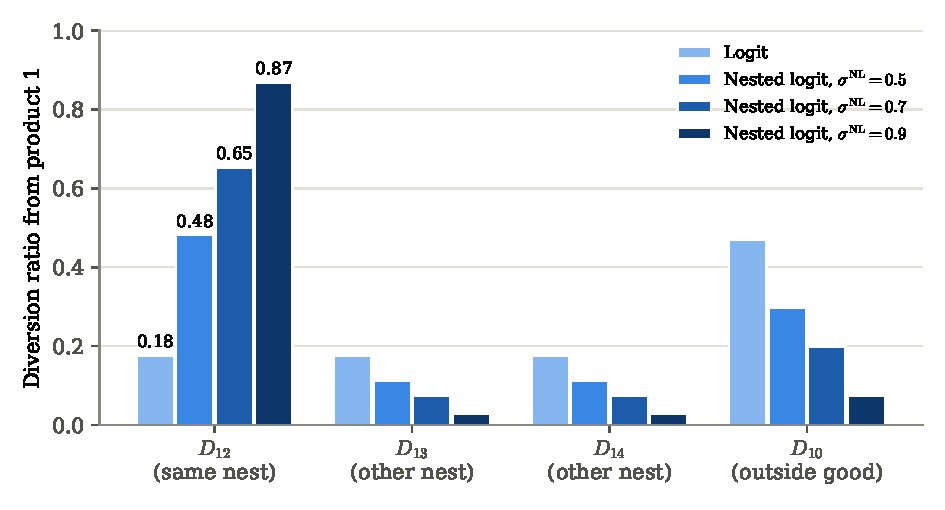
\includegraphics[width=0.95\textwidth]{figures/ch04/diversion_nl.pdf}
  \caption{Diversion ratios from product 1 in four demand models with identical shares. Products 1 and 2 form
  one nest and products 3 and 4 the other. Every inside share is 0.15 and the outside share is 0.40. The logit
  spreads lost sales in proportion to shares. The nested logit sends most of them to the other product in the
  same nest, more so as $\sigma^{\mathrm{NL}}$ rises. Computed with \texttt{figures/ch04/src/diversion\_nl.py}.}
  \label{fig:04-diversion}
\end{figure}

\subsection{What diversion ratios do not tell us}\label{sec:04-diversion-limits}

Diversion ratios are local. They are derivatives evaluated at current prices, and except under linear demand
they change when prices change. A merger moves prices, so diversion at the post-merger prices differs from the
pre-merger value that enters UPP. \Cref{ex:04-upp-linear} shows that even with constant diversion the full
price effect differs from UPP by a factor that depends on $D$.

Diversion ratios give the direction of the pricing incentive. The size of the price change also requires
pass-through, which depends on the curvature of demand (\cref{prop:04-passthrough}, \cref{ch:theory}). For a
single-product firm facing a fixed rival price, pass-through is $\frac{1}{2}$ with linear demand, $1 - s_j$
with logit demand and $\frac{\varepsilon}{\varepsilon - 1} > 1$ with constant-elasticity demand. The same UPP
can therefore produce very different price increases. \citet[Section 3]{FarrellShapiro2010} use this point to
argue that a screen should rely on the sign of pricing pressure, leaving magnitudes to a later stage.

Diversion is directional. When $\Delta$ is symmetric, \eqref{eq:04-diversion-def} implies
$-D_{12}\,\partial_1 q_1 = \partial_1 q_2 = \partial_2 q_1 = -D_{21}\,\partial_2 q_2$, so
$D_{21} = D_{12}\frac{\partial_1 q_1}{\partial_2 q_2}$. Under logit $D_{12} = \frac{s_2}{1 - s_1}$ and
$D_{21} = \frac{s_1}{1 - s_2}$: diversion from a small product to a large one exceeds diversion in the
reverse direction. A merger between a large and a small firm thus creates more pressure on the small firm's
price, for given margins.

Finally, diversion ratios describe demand for a fixed set of products and fixed non-price attributes. They are
silent about entry, repositioning and changes in quality after a merger (\cref{ch:mergers}). When diversion
comes from a demand system rather than from direct evidence, it inherits the system's restrictions. Under
logit, ``measured'' diversion restates an assumption about substitution.

\section{Existence, uniqueness and multiplicity of price equilibria}\label{sec:04-existence}

The pricing rules of \cref{sec:04-bertrand,sec:04-diversion} are first-order conditions. They describe an
equilibrium only if an equilibrium exists and if each firm's first-order condition identifies a global profit
maximum. They predict a single outcome only if the equilibrium is unique. This section asks when these
properties hold. We first explain why existence is a problem in price games with differentiated products. Next
we give conditions on demand that make profit quasi-concave and present the existence theorem of
\citet{CaplinNalebuff1991}. Finally we prove uniqueness for the logit model with any ownership structure and
construct a simple market with two equilibria. Throughout we take the set of products and their characteristics
as given. This is the first of the two branches of theory described in \cref{sec:04-why-division}, and product
choice waits until \cref{sec:04-location}.

\subsection{The existence problem}\label{sec:04-existence-problem}

Consider $F$ firms. Firm $f$ chooses the prices $p_{\mathcal{J}_f}$ of its products from a compact box
$P_f = \prod_{j \in \mathcal{J}_f}[\underline{p}_j, \bar{p}_j]$ and earns $\pi_f(p)$. A \emph{pure-strategy
Bertrand-Nash equilibrium} is a fixed point of the best-response correspondence
$BR(p) = \prod_f BR_f(p_{-\mathcal{J}_f})$, where
$BR_f(p_{-\mathcal{J}_f}) = \argmax_{p_{\mathcal{J}_f} \in P_f}\pi_f(p_{\mathcal{J}_f}, p_{-\mathcal{J}_f})$.
The standard tool is \emph{Kakutani's fixed-point theorem}. A correspondence from a nonempty, compact, convex
subset of $\R^J$ into itself has a fixed point if it has a closed graph and nonempty convex values.

Two of these requirements are usually easy. Berge's maximum theorem concerns a continuous function of a choice
variable and a parameter, maximized over a fixed compact set. It says that the maximizers, as a correspondence of
the parameter, have nonempty compact values and a closed graph. If demand is continuous, profit is continuous, and
the theorem applies to each firm's best response. The difficulty is convexity. The best-response set
is convex when $\pi_f$ is \emph{quasi-concave} in the firm's own prices, that is, when its upper contour sets
are convex. Without restrictions on demand, quasi-concavity can fail. A firm may prefer either a high price
aimed at a small group of consumers for whom its product is well positioned or a low price aimed at the mass
market. Both can dominate every intermediate price \citep[p.~2]{CaplinNalebuff1991}. The best response then
jumps between two prices, and the jump can leave the best-response map without a fixed point.
\Cref{ex:04-multiple-eq} below builds such a profit function. Here and throughout the chapter, page, proposition,
theorem, example and footnote numbers for \citet{CaplinNalebuff1991} refer to the version we checked, Cowles
Foundation Discussion Paper 937 (February 1990). The published article may number them differently.

Continuity can fail as well. In Hotelling's model with linear transport costs, a firm that undercuts its rival
by more than the transport cost between them captures the rival's entire market, so demand jumps.
\citet{DAspremontGabszewiczThisse1979} showed that this discontinuity rules out a pure-strategy price
equilibrium when the firms are close together (\cref{sec:04-location}). Mixed-strategy equilibria exist in
such discontinuous games \citep{DasguptaMaskin1986}, and \citet{OsbornePitchik1987} computed them for
Hotelling's model. Their complexity, however, rules out the comparative statics that applications need
\citep[p.~2]{CaplinNalebuff1991}.

Before \citet{CaplinNalebuff1991}, positive results came from special models in which demand is concave in own
price or log price \citep{GabszewiczThisse1979,ShakedSutton1982,Lane1980,Hauser1988,Economides1989}. These
models are one-dimensional and have consumers distributed uniformly over the market. We will see below that
concavity of demand is too strong a condition to go further.

\subsection{Sufficient conditions on demand*}\label{sec:04-existence-demand}

This subsection collects conditions on a firm's residual demand that make its profit quasi-concave in own price.
Consider a single-product firm with constant marginal cost $c$. Fix the rivals' prices and write $q(p)$ for its
residual demand, assumed nonincreasing in its own price $p$. Let $\bar p$ be the price at which demand reaches
zero, possibly $+\infty$, so that $q > 0$ exactly on $(-\infty, \bar p)$. Profit is $\pi(p) = (p - c)\,q(p)$.

Prices below cost never matter for quasi-concavity. For $p < c$ profit is nonpositive and nondecreasing,
because a higher price reduces both sales and the loss per unit. Formally, where $q$ is differentiable,
$\pi'(p) = q(p) + (p - c)q'(p) \ge 0$ for $p < c$, since $q \ge 0$, $p - c < 0$ and $q' \le 0$. Every result
below therefore concerns prices $p \ge c$.

\begin{lemma}[Log-concave demand]\label{lem:04-logconcave}
If $\ln q$ is concave on $(c, \bar p)$, then $\pi$ is quasi-concave in $p$, and the set of profit-maximizing
prices, when nonempty, is a closed interval. If $\ln q$ is strictly concave there, the maximizer is unique.
\end{lemma}

\begin{proof}
On $(c, \bar p)$ profit is positive and
\[
  \ln \pi(p) = \ln(p - c) + \ln q(p).
\]
The first term is concave in $p$ and the second is concave by assumption. A sum of concave functions is
concave, so $\pi$ is log-concave on $(c, \bar p)$. A log-concave function is quasi-concave, because its upper
contour sets are those of the concave function $\ln\pi$. Outside $(c, \bar p)$ profit is nonpositive, and it is
nondecreasing below $c$. Hence for any $t > 0$ the upper contour set $\{p : \pi(p) \ge t\}$ is a subset of
$(c, \bar p)$ and an interval. For $t \le 0$ it contains every price above $c$, and with the prices below $c$ at
which $\pi \ge t$ it forms a half-line. All upper contour sets are intervals, which is quasi-concavity. If a maximum exists
and $q$ is positive somewhere above $c$, the maximum is positive, so the argmax is an upper contour set of the concave function
$\ln\pi$, a closed interval. Strict concavity of $\ln q$ makes $\ln\pi$ strictly concave, so the maximizer is
unique.
\end{proof}

The next condition is weaker. It requires only that $\frac{1}{q}$ be convex.

\begin{lemma}[Convex reciprocal demand]\label{lem:04-recip}
If $\frac{1}{q}$ is convex on $(-\infty, \bar p)$, then $\pi$ is quasi-concave in $p$
\citep[Proposition 3]{CaplinNalebuff1991}.
\end{lemma}

\begin{proof}
We follow \citet[p.~29]{CaplinNalebuff1991}.
Suppose $\pi$ is not quasi-concave. Then there are prices $p_0 < p_1$ and $\lambda \in (0,1)$ such that, with
$p_\lambda = \lambda p_0 + (1 - \lambda)p_1$,
\[
  \pi(p_0) > \pi(p_\lambda) \qquad\text{and}\qquad \pi(p_1) > \pi(p_\lambda).
\]
By the argument above, $p_0 \ge c$, since otherwise $p_\lambda$ would earn at least as much as $p_0$. Hence
$p_\lambda > c$. If $q(p_1) = 0$, then $\pi(p_1) = 0 > \pi(p_\lambda)$ requires $p_\lambda < c$, a contradiction.
So $q(p_1) > 0$, and because $q$ is nonincreasing, $q(p_0) \ge q(p_\lambda) \ge q(p_1) > 0$. Divide the first
inequality by $q(p_0)q(p_\lambda)$ and the second by $q(p_1)q(p_\lambda)$:
\[
  \frac{p_0 - c}{q(p_\lambda)} > \frac{p_\lambda - c}{q(p_0)}, \qquad \frac{p_1 - c}{q(p_\lambda)} > \frac{p_\lambda - c}{q(p_1)}.
\]
Multiply the first by $\lambda$, the second by $1 - \lambda$, and add. The left side sums to
$\frac{p_\lambda - c}{q(p_\lambda)}$, so
\[
  \frac{p_\lambda - c}{q(p_\lambda)} > (p_\lambda - c)\Bigl[\frac{\lambda}{q(p_0)} + \frac{1 - \lambda}{q(p_1)}\Bigr].
\]
Dividing by $p_\lambda - c > 0$ gives
$\frac{1}{q(p_\lambda)} > \frac{\lambda}{q(p_0)} + \frac{1 - \lambda}{q(p_1)}$, which contradicts the convexity of
$\frac{1}{q}$.
\end{proof}

Convexity of $\frac{1}{q}$ has a familiar meaning. Let $P(\cdot)$ be the inverse demand function, so that
revenue as a function of quantity is $Q\,P(Q)$. For twice differentiable demand,
\[
  \frac{\dd^2}{\dd p^2}\Bigl(\frac{1}{q}\Bigr) = \frac{2q'^2 - q\,q''}{q^3},
  \qquad
  \frac{\dd^2}{\dd Q^2}\bigl(Q\,P(Q)\bigr) = 2P' + QP'' = \frac{2q'^2 - q\,q''}{q'^3},
\]
where the second expression uses $P' = \frac{1}{q'}$ and $P'' = -\frac{q''}{q'^3}$, evaluated at $Q = q(p)$.
Since $q > 0$ and $q' < 0$, the first is nonnegative exactly when the second is nonpositive. Convex reciprocal
demand is concave revenue in quantity. \citet[p.~14 and footnote 11]{CaplinNalebuff1991} observe that concavity of
revenue is equivalent to quasi-concavity of profit for every convex cost function, so the condition is as weak
as possible if costs are unrestricted.

A third condition works with logarithms of both price and quantity. It covers demand curves that
\cref{lem:04-recip} handles only at the boundary, such as CES demand.

\begin{lemma}[Log-log concave demand]\label{lem:04-loglog}
Let $c \ge 0$. If $\ln q$ is a concave function of $\ln p$ where $q > 0$, then $\pi$ is quasi-concave on the set
of prices where it is positive \citep[Proposition 11]{CaplinNalebuff1991}.
\end{lemma}

\begin{proof}
Write $x = \ln p$. Where profit is positive,
\[
  \ln \pi = \ln(e^x - c) + \ln q(e^x).
\]
The second term is concave in $x$ by assumption. The first has derivative $\frac{e^x}{e^x - c} = 1 + \frac{c}{e^x - c}$,
which is nonincreasing in $x$ when $c \ge 0$, so it is concave. Hence $\pi$ is log-concave, and so
quasi-concave, as a function of $\ln p$. Quasi-concavity of a function of one variable means that its upper
contour sets are intervals. The map $p \mapsto \ln p$ is increasing and sends intervals to intervals, so $\pi$ is
quasi-concave in $p$ as well.
\end{proof}

Since $\frac{\dd\ln q}{\dd\ln p} = -\varepsilon(p)$, the condition of \cref{lem:04-loglog} says that the
elasticity of demand is nondecreasing in price. Three examples locate the conditions. Linear demand
$q = a - bp$ is concave, hence log-concave. The logit residual demand
$s_j(p_j) = \frac{e^{v - \alpha p_j}}{\Phi_{-j} + e^{v - \alpha p_j}}$, with $v$ the price-free part of mean
utility, satisfies $\frac{\dd\ln s_j}{\dd p_j} = -\alpha(1 - s_j)$ and
$\frac{\dd^2\ln s_j}{\dd p_j^2} = -\alpha^2 s_j(1 - s_j) < 0$, so it is strictly log-concave.
Constant-elasticity demand $q = Ap^{-\varepsilon}$ with $\varepsilon > 1$ is log-convex, since
$\frac{\dd^2\ln q}{\dd p^2} = \frac{\varepsilon}{p^2} > 0$. Yet $\frac{1}{q} = \frac{p^\varepsilon}{A}$ is convex,
and $\ln q = \ln A - \varepsilon\ln p$ is linear in $\ln p$, so \cref{lem:04-recip,lem:04-loglog} both apply.
Cobb-Douglas demand $q = \frac{1}{p}$ sits on the boundary of both: $\frac{1}{q} = p$ and $\ln q = -\ln p$ are
linear \citep[p.~22]{CaplinNalebuff1991}. The same curvature conditions govern pass-through: log-concave demand
implies pass-through below one (\cref{ch:theory}).

A single family of concavity notions orders these conditions and also describes distributions of consumer
tastes. \Cref{app:math} develops it with proofs (\cref{def:B-rhoconcave,lem:B-rho-hierarchy}), and we restate
what this chapter needs. For $\varrho \in [-\infty, \infty]$, $\lambda \in [0,1]$ and $a, b \ge 0$, the
\emph{power mean} is $\mathcal{M}_\varrho(a, b; \lambda) = [\lambda a^\varrho + (1 - \lambda)b^\varrho]^{\frac{1}{\varrho}}$
for $\varrho \neq 0$, with the limits $\mathcal{M}_0 = a^\lambda b^{1 - \lambda}$, $\mathcal{M}_\infty = \max\{a, b\}$
and $\mathcal{M}_{-\infty} = \min\{a, b\}$. A function $\psi \ge 0$ with convex support $B \subset \R^L$ is
\emph{$\varrho$-concave} if for all $\nu_0, \nu_1 \in B$ and $\lambda \in [0,1]$,
\[
  \psi(\lambda\nu_0 + (1 - \lambda)\nu_1) \ge \mathcal{M}_\varrho\bigl(\psi(\nu_0), \psi(\nu_1); \lambda\bigr),
\]
where for $\varrho < 0$ the inequality is only required when $\psi(\nu_0)\psi(\nu_1) > 0$
\citep[p.~5]{CaplinNalebuff1991}. \Citet{CaplinNalebuff1991} write $\rho$ for the index, a symbol this book
reserves for pass-through.

For $\varrho > 0$, $\varrho$-concavity means that $\psi^\varrho$ is concave. For $\varrho < 0$ it means that $\psi^\varrho$ is convex. The
case $\varrho = 1$ is ordinary concavity, $\varrho = 0$ is log-concavity, $\varrho = -\infty$ is quasi-concavity, and
$\varrho = +\infty$ forces $\psi$ to be constant on its support, the uniform case. Power means are nondecreasing in
$\varrho$, so a $\varrho$-concave function is $\varrho'$-concave for every $\varrho' < \varrho$. Applied to demand as a function of own price,
the conditions above form a chain, with $\varrho$ equal to $1$, $0$, $-1$ and $-\infty$ from left to right:
\[
  \text{concave} \;\Longrightarrow\; \text{log-concave} \;\Longrightarrow\; \frac{1}{q}\ \text{convex} \;\Longrightarrow\; \text{quasi-concave}.
\]
\Cref{lem:04-recip} says that $(-1)$-concave demand gives quasi-concave profit. The question becomes which
primitives of consumer preferences produce $(-1)$-concave demand.

\subsection{The Caplin-Nalebuff existence theorem*}\label{sec:04-cn}

\citet{CaplinNalebuff1991} answer this question for a large family of models. Their central result is that a
pure-strategy price equilibrium exists for any number of single-product firms selling any set of products, with
products differentiated in any number of dimensions. Products that every consumer regards as identical also need a
rule for splitting tied buyers, which \cref{thm:04-cn-existence} states. The conditions restrict individual preferences and the
distribution of preferences across consumers. They cover location models, the characteristics approach and
probabilistic choice models, including the logit, probit and random coefficients models of
\cref{ch:discrete,ch:logit,ch:blp}. We present the model, the two assumptions, the aggregation theorem that
drives the result and the proofs of the main steps.

\casehead{Model}
There are $J$ firms, and firm $j$ sells one product with characteristics $x_j \in X \subset \R^K$ at constant
marginal cost $c_j$. Characteristics are fixed when firms set prices simultaneously. Each consumer buys one unit
of exactly one product. Initially all consumers have the same income $y > 0$ and there is no outside good.
Consumers have preferences over a product's characteristics $x$ and a numeraire $z$. In this subsection $z$
denotes the numeraire, and a consumer who buys product $j$ consumes $z = y - p_j$. Preferences differ across
consumers through a \emph{type} $\nu \in \R^L$, with utility $U(\nu, x, z)$. Types have density $\psi$ with
support $B$. We normalize the mass of consumers to one. In this subsection $L$ is the dimension of the type
space, which \citet{CaplinNalebuff1991} call the dimension of the market. It is unrelated to the Lerner index.

\begin{assumption}[A1, preferences linear in the type]\label{ass:04-cn-a1}
Utility takes the form
\begin{equation}\label{eq:04-cn-a1}
  U(\nu, x, z) = \sum_{l=1}^L \nu_l\,t_l(x) + g(z)\,t_{L+1}(x) + t_{L+2}(x),
\end{equation}
where $t = (t_1, \dots, t_{L+2}) : X \to \R^{L+2}$, $g$ is strictly increasing and concave, and $t_{L+1}(x) > 0$.
\end{assumption}

All consumers agree on the \emph{benefits} $t_l(x)$ that a product provides. They differ in the weights $\nu_l$
they attach to the first $L$ benefits. The benefit $t_{L+1}$ scales the utility of money, and $t_{L+2}$ is valued
equally by all. In most applications the $l$-th benefit depends only on the $l$-th characteristic and $K = L$
\citep[p.~5]{CaplinNalebuff1991}.

\begin{assumption}[A2, concavity of the type density]\label{ass:04-cn-a2}
The density $\psi$ is $\varrho$-concave with $\varrho = -\frac{1}{L+1}$, on a convex support $B \subset \R^L$ with positive
volume.
\end{assumption}

Since $-\frac{1}{L+1} < 0$, every log-concave density satisfies A2. A2 should be read jointly with A1: it suffices
that some parameterization of preferences satisfies both \citep[p.~6]{CaplinNalebuff1991}.
\Cref{tab:04-cn-coverage} lists the cases that \citet{CaplinNalebuff1991} show to be covered.

\begin{table}[htbp]
  \centering
  \caption{Distributions and utility functions covered by Assumptions A1 and A2}
  \label{tab:04-cn-coverage}
  \small
  \begin{tabularx}{\textwidth}{@{}>{\raggedright\arraybackslash}p{0.36\textwidth}>{\raggedright\arraybackslash}X@{}}
    \toprule
    \multicolumn{2}{@{}l}{\textit{Panel A. Type densities that satisfy A2}}\\
    \midrule
    Log-concave densities ($\varrho = 0$) & Multivariate beta, Dirichlet, exponential, gamma, Laplace, normal, uniform, Weibull and Wishart, with the parameter restrictions of \citet{Prekopa1971} where log-concavity requires them\\
    Beyond log-concavity & Multivariate $t$ with $a \ge 1$ degrees of freedom, including the Cauchy ($a = 1$), and Pareto and $F$ under the parameter conditions of \citet{Borell1975}. These families are $\bigl(-\frac{1}{L}\bigr)$-concave, and A2 restricts their parameters\\
    Transformations & Any truncation to a convex set of a density above\\
    Excluded & Lognormal\\
    \midrule
    \multicolumn{2}{@{}l}{\textit{Panel B. Utility functions that satisfy A1}}\\
    \midrule
    CES in characteristics & $U = \sum_l \nu_l x_l^{\eta} + z^{\eta}$\\
    Linear in characteristics ($\eta = 1$) & $U = \beta x^{o} + \nu x^{u} + z$, observed $x^{o}$, unobserved $x^{u}$: logit, probit and random coefficients models (Example 3.2)\\
    Cobb-Douglas & $U = \sum_l \nu_l\ln x_l + \ln z$, or $U = \sum_l \nu_l\ln x_l + z$\\
    Quadratic transport costs & $U = -\|x - \nu\|^2 + z$, linear in $\nu$ after expanding the square\\
    Vertical differentiation & $U = x(z + \nu)$, $\nu \in \R$\\
    Direct translog & $U = g(z) + \sum_k \nu_k\ln x_k + \frac{1}{2}\sum_k\sum_l \nu_{kl}\ln x_k\ln x_l$, with $L = \frac{K(K+3)}{2}$\\
    Johansen additive utility & Covered after a change of variables (Example 3.3)\\
    Not covered & Hotelling's linear distance, $U = z - |\nu - x|$, whose demand is discontinuous\\
    \bottomrule
  \end{tabularx}
  \par\smallskip
  \begin{minipage}{\textwidth}\footnotesize
  Notes: $\eta$ denotes the CES exponent in Panel B. Example numbers refer to \citet{CaplinNalebuff1991}. In
  Example 3.2 the unobserved characteristics are unit vectors, so $\nu_j$ is a consumer's idiosyncratic taste for
  product $j$. Logit takes the $\nu_j$ to be i.i.d.\ type-I extreme value (which \citet{CaplinNalebuff1991} call
  Weibull) and probit takes them to be normal. Random coefficients on observed characteristics enter linearly and
  are covered when their density satisfies A2. Source: \citet[pp.~6--9]{CaplinNalebuff1991}.
  \end{minipage}
\end{table}

Two entries need comment. Logit fits A1 through Example 3.2: with one unobserved characteristic per product,
$U(\nu, x_j, z) = \beta x^{o}_j + \nu_j + z$, and the type vector collects the product-specific tastes. The type-I
extreme value density $e^{-u}\exp(-e^{-u})$ has $\frac{\dd^2}{\dd u^2}\ln(\cdot) = -e^{-u} < 0$, so a product of
independent such densities is log-concave and satisfies A2. Models with a random price coefficient,
$u_{ij} = x_j\beta_i - \alpha_i p_j + \epsilon_{ij}$, are covered only after dividing utility by $\alpha_i$. The
transformed utility $\frac{x_j\beta_i + \epsilon_{ij}}{\alpha_i} - p_j$ is linear in the money-metric types
$\frac{\beta_i}{\alpha_i}$ and $\frac{\epsilon_{ij}}{\alpha_i}$, so A1 holds with $g(z) = z$. A2 then restricts the
distribution of these ratios, which need not be $\varrho$-concave. \Cref{ex:04-multiple-eq} exploits exactly this
gap.

\casehead{Reservation prices and demand}
Because utility is strictly increasing in $z$, each type has a reservation price for each product. Fix the
other prices $p_{-j}$ and let $\bar U_j(\nu) = \max_{k \neq j}U(\nu, x_k, y - p_k)$ be the best alternative.
The reservation price of type $\nu$ for product $j$ is
\[
  R_j(\nu; p_{-j}) =
  \begin{cases}
    y & \text{if } U(\nu, x_j, 0) \ge \bar U_j(\nu),\\
    y - z_j & \text{if } U(\nu, x_j, z_j) = \bar U_j(\nu) \text{ has a solution } z_j,\\
    -\infty & \text{if } U(\nu, x_j, z) < \bar U_j(\nu) \text{ for all } z.
  \end{cases}
\]
Type $\nu$ buys $j$ exactly when $p_j \le R_j(\nu; p_{-j})$, up to ties. Demand for product $j$ is the mass of
types whose reservation price exceeds the price,
\begin{equation}\label{eq:04-cn-demand}
  q_j(p_j) = \int_{\{\nu \,:\, R_j(\nu;\, p_{-j}) \ge p_j\}}\psi(\nu)\,\dd\nu,
\end{equation}
which is equation (4.1) of \citet{CaplinNalebuff1991}. Given rivals' prices, firm $j$ faces a monopoly problem
with a population of reservation prices, and \eqref{eq:04-cn-demand} is nonincreasing in $p_j$.

Call products $j$ and $k$ \emph{distinct} if their benefit vectors $(t_1, \dots, t_L)$ differ, and
\emph{equivalent} if $t(x_j) = t(x_k)$. Demand is continuous in all prices when products are distinct
\citep[Proposition 1]{CaplinNalebuff1991}.
\citeauthor{CaplinNalebuff1991} state the condition as $t(x_j) \neq t(x_k)$, and their proof uses the first $L$
benefits. Under A1 the types indifferent between $j$ and $k$ satisfy one linear equation in $\nu$,
\[
  \sum_{l=1}^L \nu_l\,[t_l(x_k) - t_l(x_j)] = b_{jk}(p_j, p_k),
\]
with $b_{jk} = t_{L+2}(x_j) - t_{L+2}(x_k) + t_{L+1}(x_j)g(y - p_j) - t_{L+1}(x_k)g(y - p_k)$. This set is a
hyperplane, which has zero mass under a density. Each consumer's demand jumps at her reservation price, but the
population smooths the jumps away. Hotelling's linear-distance model fails this test: its demand jumps even for
distinct products, so no transformation of it can satisfy A1 and A2 \citep[p.~9]{CaplinNalebuff1991}.

\casehead{Aggregation}
The key step is to show that the integral in \eqref{eq:04-cn-demand} inherits concavity from $\psi$. For sets
$A_0, A_1 \subset \R^L$ and $\lambda \in [0,1]$, the \emph{Minkowski average} is
$A_\lambda = \lambda A_0 + (1 - \lambda)A_1 = \{\lambda a_0 + (1 - \lambda)a_1 : a_0 \in A_0,\, a_1 \in A_1\}$.
The tool is the Pr\'ekopa-Borell theorem, which \cref{thm:B-prekopa-borell} states in full. Let $\psi$ be a
probability density on $\R^L$ with convex support $B$, and let $A_0$ and $A_1$ be measurable sets that intersect
$B$. If $\psi$ is $\varrho$-concave with $\varrho \ge -\frac{1}{L}$, then for every $\lambda \in [0,1]$,
\begin{equation}\label{eq:04-prekopa-borell}
  \int_{A_\lambda}\psi(\nu)\,\dd\nu \;\ge\;
  \Bigl[\lambda\Bigl(\int_{A_0}\psi\Bigr)^{\varrho^*} + (1 - \lambda)\Bigl(\int_{A_1}\psi\Bigr)^{\varrho^*}\Bigr]^{\frac{1}{\varrho^*}},
  \qquad \varrho^* = \frac{\varrho}{1 + L\varrho}.
\end{equation}
The theorem is due to \citet{Prekopa1971} for log-concave densities and to \citet{Borell1975} in general.
\citet{DasGupta1980} gives proofs and the history, and \citet[p.~11]{CaplinNalebuff1991} state it in this form.
The right side of \eqref{eq:04-prekopa-borell} is the power mean $\mathcal{M}_{\varrho^*}$ of the two
probabilities. A $\varrho$-concave density thus defines a $\varrho^*$-concave measure over sets. Three cases help.
A uniform density ($\varrho = \infty$) gives $\varrho^* = \frac{1}{L}$, the Brunn-Minkowski inequality
$\mathrm{vol}(A_\lambda)^{\frac{1}{L}} \ge \lambda\,\mathrm{vol}(A_0)^{\frac{1}{L}} + (1 - \lambda)\,\mathrm{vol}(A_1)^{\frac{1}{L}}$.
A log-concave density ($\varrho = 0$) gives a log-concave measure ($\varrho^* = 0$). As $\varrho$ falls to $-\frac{1}{L}$, $\varrho^*$
falls to $-\infty$, so only quasi-concavity survives. Since $\frac{\dd \varrho^*}{\dd \varrho} = \frac{1}{(1 + L\varrho)^2} > 0$,
more concave densities give more concave measures.

\begin{theorem}[Concavity of demand]\label{thm:04-cn-demand}
Suppose A1 holds, $\psi$ is $\varrho$-concave with $\varrho \ge -\frac{1}{L}$ on a convex support, and products are
distinct. Then each firm's demand is $\varrho^*$-concave in its own price, with $\varrho^* = \frac{\varrho}{1 + L\varrho}$, on
the interval of prices where demand is positive \citep[Theorem 1]{CaplinNalebuff1991}.
\end{theorem}

\begin{proof}
Fix $p_{-j}$ and let $\mathcal{A}_j(p_j)$ be the set of types who weakly prefer $j$ at price $p_j$ to every other
product. Take prices $p_0$ and $p_1$ with positive demand, $\lambda \in [0,1]$, and
$p_\lambda = \lambda p_0 + (1 - \lambda)p_1$. Let $\nu_0 \in \mathcal{A}_j(p_0)$ and $\nu_1 \in \mathcal{A}_j(p_1)$.
By A1, for every $k \neq j$,
\begin{align*}
  \sum_l \nu_{0l}t_l(x_j) + g(y - p_0)t_{L+1}(x_j) + t_{L+2}(x_j) &\ge \sum_l \nu_{0l}t_l(x_k) + g(y - p_k)t_{L+1}(x_k) + t_{L+2}(x_k),\\
  \sum_l \nu_{1l}t_l(x_j) + g(y - p_1)t_{L+1}(x_j) + t_{L+2}(x_j) &\ge \sum_l \nu_{1l}t_l(x_k) + g(y - p_k)t_{L+1}(x_k) + t_{L+2}(x_k).
\end{align*}
Multiply the first line by $\lambda$, the second by $1 - \lambda$, and add. Both sides are affine in the type,
and $p_k$ is the same in both lines, so with $\nu_\lambda = \lambda\nu_0 + (1 - \lambda)\nu_1$,
\begin{multline*}
  \sum_l \nu_{\lambda l}t_l(x_j) + \bigl[\lambda g(y - p_0) + (1 - \lambda)g(y - p_1)\bigr]t_{L+1}(x_j) + t_{L+2}(x_j)\\
  \ge \sum_l \nu_{\lambda l}t_l(x_k) + g(y - p_k)t_{L+1}(x_k) + t_{L+2}(x_k).
\end{multline*}
Concavity of $g$ gives $g(y - p_\lambda) \ge \lambda g(y - p_0) + (1 - \lambda)g(y - p_1)$, and $t_{L+1}(x_j) > 0$.
Replacing the bracket by $g(y - p_\lambda)$ therefore raises the left side, so type $\nu_\lambda$ weakly prefers
$j$ at price $p_\lambda$. We have shown
\[
  \mathcal{A}_j(p_\lambda) \supseteq \lambda\mathcal{A}_j(p_0) + (1 - \lambda)\mathcal{A}_j(p_1).
\]
Ties have zero mass because products are distinct, so $q_j(p) = \int_{\mathcal{A}_j(p)}\psi$.
Monotonicity of the integral and the Pr\'ekopa-Borell inequality \eqref{eq:04-prekopa-borell} give
\[
  q_j(p_\lambda) \ge \int_{\lambda\mathcal{A}_j(p_0) + (1 - \lambda)\mathcal{A}_j(p_1)}\psi
  \ge \mathcal{M}_{\varrho^*}\bigl(q_j(p_0), q_j(p_1); \lambda\bigr),
\]
which is $\varrho^*$-concavity of $q_j$ in $p_j$ \citep[p.~28]{CaplinNalebuff1991}.
\end{proof}

The proof uses A1 in one place: the set of buyers at an intermediate price contains the Minkowski average of the
buyer sets at the two end prices. Linearity in $\nu$ lets the two preference inequalities be averaged, and concavity
of $g$ handles the price.

\begin{example}[Uniform types on a simplex]\label{ex:04-cn-simplex}
Let types be uniform on the $L$-dimensional unit simplex $\{\nu \ge 0 : \sum_l\nu_l \le 1\}$ and let reservation
prices be $R(\nu) = 1 - \sum_l\nu_l$ \citep[Example 4.1]{CaplinNalebuff1991}. This arises, for example, from
$U = \sum_l \nu_l x_l + z$ when a rival product with characteristics $(1, \dots, 1)$ sells at price 1 and our
product has characteristics $(0, \dots, 0)$. At price $p \in [0,1]$ the buyers are the types with
$\sum_l\nu_l \le 1 - p$, a copy of the simplex scaled by $1 - p$. Its volume is $(1 - p)^L$ times the volume of the
simplex, so
\[
  q(p) = (1 - p)^L, \qquad q(p)^{\frac{1}{L}} = 1 - p.
\]
Demand is $\frac{1}{L}$-concave and no more, which is exactly the bound $\varrho^* = \frac{1}{L}$ of
\cref{thm:04-cn-demand} for a uniform density. The buyer set at $p_\lambda$ equals the Minkowski average of the
buyer sets at $p_0$ and $p_1$, because $\lambda(1 - p_0)T + (1 - \lambda)(1 - p_1)T = (1 - p_\lambda)T$ for the
convex simplex $T$. \Cref{fig:04-cn-simplex} draws the case $L = 2$.
\end{example}

\begin{figure}[htbp]
  \centering
  \begin{tikzpicture}[x={(-1.5cm,-1.25cm)}, y={(2.3cm,-0.95cm)}, z={(0cm,3.7cm)}, line join=round, >=Stealth]
    \draw[->, thin] (0,0,0) -- (1.3,0,0) node[below left] {$\nu_1$};
    \draw[->, thin] (0,0,0) -- (0,1.28,0) node[below right] {$\nu_2$};
    \draw[->, thin] (0,0,0) -- (0,0,1.25) node[left] {$p$};
    \fill[gray!12] (0,0,0) -- (1,0,0) -- (0,1,0) -- cycle;
    \foreach \pp/\nm in {0.2/1, 0.45/\lambda, 0.7/0} {
      \pgfmathsetmacro{\aa}{1-\pp}
      \filldraw[fill=gray!40, draw=black, thin, fill opacity=0.85]
        (0,0,\pp) -- (\aa,0,\pp) -- (0,\aa,\pp) -- cycle;
      \draw[densely dotted] (0,\aa,\pp) -- ++(0,0.5,0) node[right] {$\mathcal{A}(p_{\nm})$};
      \node[left] at (\aa,0,\pp) {$p_{\nm}$};
    }
    \draw[thick] (1,0,0) -- (0,1,0);
    \draw[thick] (0,0,1) -- (1,0,0);
    \draw[thick] (0,0,1) -- (0,1,0);
    \draw[thick] (0,0,0) -- (1,0,0);
    \draw[thick] (0,0,0) -- (0,1,0);
    \node[left] at (0,0,1) {$1$};
    \node[below] at (1,0,0) {$1$};
    \node[below] at (0,1,0) {$1$};
  \end{tikzpicture}
  \caption{Buyer sets when types are uniform on the two-dimensional simplex and $R(\nu) = 1 - \nu_1 - \nu_2$.
  At price $p$ the set of buyers $\mathcal{A}(p)$ is the triangle $\{\nu \ge 0 : \nu_1 + \nu_2 \le 1 - p\}$, which
  shrinks linearly as $p$ rises, so $q(p) = (1 - p)^2$. With $p_\lambda = \lambda p_0 + (1 - \lambda)p_1$ (here
  $\lambda = \frac{1}{2}$), the set $\mathcal{A}(p_\lambda)$ is the Minkowski average of $\mathcal{A}(p_0)$ and
  $\mathcal{A}(p_1)$. Redrawn from \citet{CaplinNalebuff1991}, Figure 1.}
  \label{fig:04-cn-simplex}
\end{figure}

A concave density behaves like an extra dimension of uniform types. Let $L = 1$, $\psi(\nu) = 2\nu$ on $[0,1]$
and $R(\nu) = 1 - \nu$. Then
\[
  q(p) = \int_0^{1 - p}2\nu\,\dd\nu = (1 - p)^2,
\]
the same demand as uniform types on the two-dimensional simplex \citep[Example 4.2]{CaplinNalebuff1991}. The
density is linear, hence $1$-concave, and \cref{thm:04-cn-demand} gives $\varrho^* = \frac{1}{1 + 1} = \frac{1}{2}$,
again exactly attained. More generally, a density with $\psi^{\frac{1}{n}}$ concave for a positive integer $n$
yields the bound $\frac{1}{L + n}$ of a uniform density in $L + n$ dimensions.

The bounds of \cref{thm:04-cn-demand} cannot be improved \citep[Proposition 2]{CaplinNalebuff1991}. For every
$\varrho > -\frac{1}{L}$ some model satisfies A1 with a $\varrho$-concave density and has $q^{\varrho^*}$ affine in price. Such a
demand is $\varrho^*$-concave and no more.
In the following examples $U = \sum_l\nu_lx_l + z$, our product has characteristics $(1, 0, \dots, 0)$, and a
rival with characteristics $(0, \dots, 0)$ sells at price zero. Type $\nu$ then buys our product exactly when
$\nu_1 \ge p$, so $R(\nu) = \nu_1$. In each example $\psi^\varrho$, or $\ln\psi$ when $\varrho = 0$, is affine on the support,
so $\psi$ is $\varrho$-concave.
\begin{itemize}
  \item For $\varrho > 0$, let $\psi$ be proportional to $(1 - \sum_l\nu_l)^{\frac{1}{\varrho}}$ on the unit simplex. Then
  $q(p) = (1 - p)^{\frac{1 + L\varrho}{\varrho}}$ on $[0, 1]$.
  \item For $\varrho = 0$, let $\psi(\nu) = e^{-\sum_l\nu_l}$ on $\R^L_+$. Then $q(p) = e^{-p}$.
  \item For $-\frac{1}{L} < \varrho < 0$, let $\psi$ be proportional to $(1 + \sum_l\nu_l)^{\frac{1}{\varrho}}$ on $\R^L_+$,
  which is integrable because $\frac{1}{\varrho} < -L$. Then $q(p) = (1 + p)^{\frac{1 + L\varrho}{\varrho}}$ for $p \ge 0$. It falls
  with price because the exponent is negative.
\end{itemize}
Each demand follows by integrating out $\nu_2, \dots, \nu_L$ and then $\nu_1$ from $p$ upward. In every case
$q^{\varrho^*}$ is affine in $p$, because $\frac{1 + L\varrho}{\varrho} = \frac{1}{\varrho^*}$.

The examples also show why earlier work, which assumed concave demand, could not go far. \Cref{thm:04-cn-demand}
guarantees concave demand only if $\varrho^* = 1$. Since $\varrho^* \le \frac{1}{L}$ for every $\varrho$, this guarantee holds only when
$L = 1$ and $\varrho = \infty$: a uniform distribution of consumers in a one-dimensional market
\citep[p.~14]{CaplinNalebuff1991}. The bound holds for the whole class and does not cap the concavity of each
model. In the setup of the examples above with $L = 1$, the density $\psi(\nu) = 2\nu$ on $[0,1]$ has the bound
$\varrho^* = \frac{1}{2}$, yet its demand $q(p) = 1 - p^2$ is concave.

\begin{proposition}[Quasi-concave profit]\label{prop:04-cn-quasiconcave}
Under A1 and A2, with distinct products, each firm's profit is quasi-concave in its own price
\citep[Proposition 4]{CaplinNalebuff1991}.
\end{proposition}

\begin{proof}
A2 sets $\varrho = -\frac{1}{L+1}$, which exceeds $-\frac{1}{L}$, so \cref{thm:04-cn-demand} applies. The implied
concavity index of demand is
\[
  \varrho^* = \frac{\varrho}{1 + L\varrho} = \frac{-\frac{1}{L+1}}{1 - \frac{L}{L+1}} = \frac{-\frac{1}{L+1}}{\frac{1}{L+1}} = -1.
\]
Demand is $(-1)$-concave, that is, $\frac{1}{q_j}$ is convex where $q_j > 0$. Demand is nonincreasing by
\eqref{eq:04-cn-demand}. \Cref{lem:04-recip} then gives quasi-concavity of profit.
\end{proof}

The value $\varrho = -\frac{1}{L+1}$ in A2 is thus chosen to deliver exactly $(-1)$-concave demand, the weakest
condition that guarantees quasi-concave profit. Solving $\frac{\varrho}{1 + L\varrho} = -1$ for $\varrho$ gives $\varrho = -1 - L\varrho$, so
$\varrho(1 + L) = -1$ and $\varrho = -\frac{1}{L+1}$.

\begin{theorem}[Existence]\label{thm:04-cn-existence}
Under A1 and A2, for any number of single-product firms and any products, a pure-strategy Bertrand-Nash
equilibrium exists \citep[Theorem 2]{CaplinNalebuff1991}. If some products are equivalent, the result uses the
following tie rule. Buyers who are indifferent among equivalent products at the same price buy from a lowest-cost
producer among the firms charging that price.
\end{theorem}

\begin{proof}
We follow \citet[pp.~14--15]{CaplinNalebuff1991} in three steps.

\emph{Distinct products, all costs below income.} Restrict firm $j$ to prices in $[c_j, y]$ and let
$Z = \prod_j[c_j, y]$, a nonempty, compact, convex set. Prices above $y$ sell nothing, and prices below $c_j$
earn at most zero, which the price $c_j$ also earns. Hence a maximizer on $[c_j, y]$ is a global best response.
Demand is continuous because products are distinct, so profits are continuous in all prices. By Berge's maximum
theorem, the restricted best-response correspondence has nonempty compact values and a closed graph. By
\cref{prop:04-cn-quasiconcave}, profit is quasi-concave in own price, and the set of maximizers of a
quasi-concave function on an interval is an interval. Kakutani's theorem gives a fixed point, which is an
equilibrium because every firm plays a global best response.

\emph{Equivalent products.} If several products are equivalent, all consumers buy the cheapest of them, as in
homogeneous Bertrand competition. In each such group, select a lowest-cost producer and solve the game with
distinct products among the selected firms. Each selected firm faces the added constraint that it prices no higher
than the cost of the next-lowest-cost producer in its group. Let the remaining firms price at cost. When the
constraint binds, the selected firm charges exactly that rival's cost, so the two firms tie.
The tie rule gives the buyers of the group to the selected firm, so the remaining firms sell nothing. A remaining
firm can win buyers only by pricing below the selected firm, and hence below its own cost, so it cannot gain by
deviating. The selected firm loses the group's buyers if it prices above its cap. At or below the cap its demand
equals its demand in the game among selected firms, so its fixed-point price is a global best response.

\emph{Costs above income.} Firms with $c_j > y$ can sell nothing at a profit. Solving the game without them and
letting them price at cost preserves the equilibrium.
\end{proof}

\casehead{Interpretation and related work}
The theorem holds for any number of firms and any configuration of products, with no symmetry, given the tie rule
for equivalent products. The tie rule cannot be dropped. Take two equivalent products with costs 0 and 1, sold to
a unit mass of consumers who each value either product at 2. Under an equal split of ties, the prices $(1, 1)$
give the efficient firm a profit of $\frac{1}{2}$, while the price $1 - \eta$ gives it $1 - \eta$ for small
$\eta > 0$. With continuous prices this game has no pure-strategy equilibrium, as in the asymmetric-cost Bertrand
game of \cref{sec:02-bertrand-homog}. The theorem gives
\emph{sufficient} conditions, and equilibria often exist when they fail. \citet[p.~15]{CaplinNalebuff1991} relate
their approach to the independent work of \citet{Dierker1989}. Dierker takes the joint distribution of consumers'
valuations of the products as the primitive and assumes it is log-concave. Pr\'ekopa's theorem then makes demand
log-concave. \citet{CaplinNalebuff1991} instead start from a model of the characteristics space and of preference
parameters, and derive the valuations. Their framework supplies a large set of utility models for which the
joint distribution of valuations is log-concave for every set of products.

\casehead{Extensions}
\citet[Section 8]{CaplinNalebuff1991} extend the result in several directions. We summarize them briefly.
\begin{itemize}
  \item \emph{Unequal incomes.} Income enters as an additional type. Assumption A1$'$ of
  \citet[p.~20]{CaplinNalebuff1991} is A1 with $g(z) = z$. Then the reservation price of type $(\nu, y)$ for
  product $j$ is
  \[
    R_j(\nu, y) = y + \frac{\nu\cdot\bm{t}_j + t_{L+2}(x_j) - \max_{k \neq j}\bigl[\nu\cdot\bm{t}_k + (y - p_k)t_{L+1}(x_k) + t_{L+2}(x_k)\bigr]}{t_{L+1}(x_j)},
  \]
  with $\bm{t}_j = (t_1(x_j), \dots, t_L(x_j))$. A maximum of affine functions is convex, so $R_j$ is concave in
  $(\nu, y)$. The buyer sets therefore satisfy the Minkowski inclusion of the proof of \cref{thm:04-cn-demand},
  now in $\R^{L+1}$. Assumption A2$'$ requires the joint density of types and income to be
  $\bigl(-\frac{1}{L+2}\bigr)$-concave on a convex support in $\R^{L+1}$, with bounded income. With $L + 1$ in
  place of $L$, the computation in the proof of \cref{prop:04-cn-quasiconcave} again gives $\varrho^* = -1$, and an
  equilibrium exists (their Proposition 10). The vertical model $U = xz$
  \citep{GabszewiczThisse1979,ShakedSutton1982} is a special case. Uniqueness extends as well. Under A1$'$, if the
  logarithm of the joint density is concave and differentiable where the density is positive, the duopoly
  equilibrium is unique and the pricing game is log-supermodular. Pure vertical differentiation, with identical
  preferences and different incomes, is the one-dimensional case of their Proposition 7 (p.~20).
  \item \emph{An outside good.} Add a fictitious firm 0 selling $x_0 = 0$ at the fixed price $p_0 = 0$. Existence
  is unaffected, but the duopoly uniqueness result below no longer applies, because the market becomes a
  three-firm oligopoly. In location models the product $x_0 = 0$ is a differentiated product located at the origin,
  not the absence of consumption. Non-purchase can still be modeled by a utility loss from buying nothing that is
  concave in the type (pp.~20--21).
  \item \emph{Variable and non-exclusive demand.} The reservation-price argument no longer applies. With
  individual demands $d_j(\nu, y, p_j)$, aggregate demand is $\int \psi(\nu, y)\,d_j(\nu, y, p_j)\,\dd\nu\,\dd y$.
  \citet{Prekopa1973} shows that integrating a jointly log-concave function over some of its arguments yields a
  log-concave function of the rest. If $\ln d_j$ is concave in $(\nu, y, \ln p_j)$ and $\ln\psi$ is concave, aggregate
  demand is log-concave in $\ln p_j$, and \cref{lem:04-loglog} gives quasi-concave profit. Cobb-Douglas
  preferences satisfy these conditions, and an equilibrium exists with two or more firms and positive costs, unique
  in duopoly.
  \item \emph{CES.} The representative-consumer CES model generates the same demands as a discrete-continuous choice
  model with i.i.d.\ extreme value tastes \citep[eq.~(8.3)]{CaplinNalebuff1991}. Hence an equilibrium exists in the
  CES model with two or more firms and positive costs, unique in duopoly \citep[Proposition 14]{CaplinNalebuff1991}.
  \Cref{sec:04-repcons-ces,sec:04-repcons-cesdc} derive the representation and explain why one firm is not enough.
  \item \emph{Translog.} With indirect translog demands and an own-price coefficient common to all consumers,
  $\ln d_j$ is concave in its arguments, and log-concave densities give quasi-concave profit.
  \item \emph{Unbounded markets.} With infinitely many products in an unbounded space, any price vector that
  satisfies all first-order conditions, and at which A1 and A2 hold, is an equilibrium
  \citep[Proposition 15]{CaplinNalebuff1991}.
  This validates the first-order approach of \citet{Stiglitz1986} with quadratic transport costs.
\end{itemize}

\casehead{Contribution and limits}
Before \citet{CaplinNalebuff1991}, existence results required one-dimensional products, uniform consumers or
complete symmetry. Their theorem covers multi-dimensional characteristics, asymmetric products and the discrete
choice models that empirical work uses. It also brought $\varrho$-concavity and the Pr\'ekopa-Borell theorem into
industrial organization. The limits are as instructive. Each firm sells one product, and the proof does not extend
to multi-product firms, whose profit need not be quasi-concave in the vector of own prices. The density condition
excludes type distributions with separated groups of consumers, such as finite mixtures of logits with very
different price sensitivities. Products are fixed, so the theorem says nothing about product choice. Finally,
uniqueness requires more, as the next subsection shows.

Caplin and Nalebuff close by pointing to product choice as the next step (pp.~26--27). Where the equilibrium is
both existent and unique, as in the logit with any number of products and in duopoly, firms can predict their
profits for any configuration of competing products. Product design can then be studied with price competition in
the second stage. \citet{PrescottVisscher1977} had studied sequential location with fixed prices. Caplin and
Nalebuff also cite a 1989 working paper by Feenstra and Levinsohn that uses a variant of their model to map
consumer preferences for the characteristics of cars. \Cref{sec:04-location} studies product choice in the
simplest settings.

\subsection{Uniqueness}\label{sec:04-uniqueness}

Uniqueness matters for counterfactuals: a model that predicts several outcomes after a merger predicts none of
them reliably. The classical sufficient condition is a dominant diagonal of the matrix of second derivatives of
profit \citep{Friedman1977}. We state it for single-product firms.

\begin{proposition}[Diagonal dominance]\label{prop:04-diag-dominance}
Let firm $j$ choose $p_j \in P_j = [\underline{p}_j, \bar p_j]$ and let $P = \prod_j P_j$. Suppose that
\begin{enumerate}[label=(\roman*)]
  \item Each $\pi_j$ is twice continuously differentiable on an open set containing $P$.
  \item For every $p_{-j}$, $\pi_j(\cdot, p_{-j})$ has a unique maximizer $BR_j(p_{-j})$ in the interior of $P_j$,
  at which $\frac{\partial^2\pi_j}{\partial p_j^2} < 0$.
  \item At every such maximizer,
  $\sum_{k \neq j}\bigl|\frac{\partial^2\pi_j}{\partial p_j\partial p_k}\bigr| < \bigl|\frac{\partial^2\pi_j}{\partial p_j^2}\bigr|$.
\end{enumerate}
Then the best-response map $BR : P \to P$ is a contraction in the sup norm. The game has exactly one Bertrand-Nash
equilibrium, and best-response iteration converges to it from every starting point in $P$.
\end{proposition}

\begin{proof}
Best responses satisfy the first-order condition
$\frac{\partial\pi_j}{\partial p_j}(BR_j(p_{-j}), p_{-j}) = 0$. By (ii) the derivative of the left side with
respect to $p_j$ is nonzero at the maximizer, so the implicit function theorem makes $BR_j$ continuously
differentiable, with
\[
  \frac{\partial BR_j}{\partial p_k} = -\Bigl(\frac{\partial^2\pi_j}{\partial p_j^2}\Bigr)^{-1}\frac{\partial^2\pi_j}{\partial p_j\partial p_k}\,\Bigg|_{p_j = BR_j(p_{-j})}.
\]
By (iii), $\sum_{k \neq j}\bigl|\frac{\partial BR_j}{\partial p_k}\bigr| < 1$ at every $p_{-j}$. This sum is
continuous on the compact set $\prod_{k \neq j}P_k$, so its maximum $\ell_j$ is below one. Let
$\ell = \max_j\ell_j < 1$. For $p, p' \in P$, apply the mean value theorem to
$t \mapsto BR_j(p'_{-j} + t(p_{-j} - p'_{-j}))$ on $[0,1]$. For some intermediate point $\tilde p_{-j}$,
\[
  |BR_j(p_{-j}) - BR_j(p'_{-j})| \le \sum_{k \neq j}\Bigl|\frac{\partial BR_j}{\partial p_k}(\tilde p_{-j})\Bigr|\,|p_k - p'_k| \le \ell\,\|p - p'\|_\infty.
\]
Taking the maximum over $j$ gives $\|BR(p) - BR(p')\|_\infty \le \ell\|p - p'\|_\infty$. The contraction mapping
theorem (\cref{app:math}) gives a unique fixed point and convergence of the iteration $p^{(n+1)} = BR(p^{(n)})$
from any $p^{(0)} \in P$.
\end{proof}

The argument survives two changes of variables that are often useful. Best responses do not change if profit is
replaced by an increasing transformation, such as $\ln\pi_j$, or if prices are replaced by smooth increasing
functions of prices. Diagonal dominance may hold for the transformed problem when it fails for the original, and
the conclusion about uniqueness carries over. A second route avoids best responses altogether. Stack the
first-order conditions as $G(p) = 0$ with $G_j = \frac{\partial\pi_j}{\partial p_j}$. A \emph{P-matrix} is a square
matrix whose principal minors are all positive. If the Jacobian of $-G$ is a P-matrix everywhere on a rectangle,
$G$ is one-to-one there \citep{GaleNikaido1965}. The first-order conditions then have at most one solution. A matrix with positive diagonal
and strictly dominant diagonal rows is a P-matrix. Negative own second derivatives together with the inequality of (iii) at
every point of the rectangle therefore suffice.

\casehead{Uniqueness in the Caplin-Nalebuff framework}
\citet[Section 6]{CaplinNalebuff1991} establish uniqueness in three cases, in the ``differentiable case'' where $g$
is twice differentiable and $\psi$ is differentiable. In a duopoly with A1 and a log-concave type density, the
equilibrium is unique (their Proposition 6). In a one-dimensional market with a log-concave density on an interval,
there is at most one equilibrium with a given set of active firms (Proposition 7). In the logit model the
equilibrium is unique for any number of single-product firms, a result first noted for duopoly by
\citet{AndersonDePalma1988}.
Firms with zero demand create no real indeterminacy. Any equilibrium in which some firms sell nothing has a
counterpart with the same demands and profits in which those firms price at marginal cost (Proposition 5).
Uniqueness thus refers to market outcomes.

The proofs change variables from $p_j$ to the utility from money, $u_j = g(y - p_j)\,t_{L+1}(x_j)$. In a duopoly,
demand depends on the two utilities only through the difference $u_1 - u_2$. Write $\tilde q_1(u_1 - u_2)$ for firm 1's
demand and $\tilde p_1(u_1) = y - g^{-1}\bigl(\frac{u_1}{t_{L+1}(x_1)}\bigr)$ for the price that delivers $u_1$. Then
\[
  \ln\pi_1 = \ln\bigl(\tilde p_1(u_1) - c_1\bigr) + \ln \tilde q_1(u_1 - u_2).
\]
The first term is strictly concave in $u_1$ because $\tilde p_1$ is concave. The second is concave because the
Pr\'ekopa-Borell theorem makes demand log-concave in $u_1$. Because $\tilde q_1$ depends on $u_1 - u_2$ only,
\[
  \frac{\partial^2\ln \tilde q_1}{\partial u_1^2} = -\frac{\partial^2\ln \tilde q_1}{\partial u_1\partial u_2} \le 0,
  \qquad\text{so}\qquad
  \frac{\partial^2\ln\pi_1}{\partial u_1^2} < \frac{\partial^2\ln \tilde q_1}{\partial u_1^2} = -\frac{\partial^2\ln\pi_1}{\partial u_1\partial u_2}.
\]
This is diagonal dominance for $\ln\pi_1$ in the utility variables, and the remark after
\cref{prop:04-diag-dominance} gives uniqueness \citep[p.~30]{CaplinNalebuff1991}. The cross partial
$\frac{\partial^2\ln\pi_1}{\partial u_1\partial u_2}$ is nonnegative, which is the next property.

\casehead{Log-supermodularity}
A positive payoff $\pi_j(p_j, p_{-j})$ is \emph{log-supermodular} if $\ln\pi_j$ has increasing differences in
$(p_j, p_k)$ for every $k \neq j$. For smooth payoffs this means
$\frac{\partial^2\ln\pi_j}{\partial p_j\partial p_k} \ge 0$: a higher rival price raises the marginal return, in
logs, to a higher own price. A price game with interval strategy sets and log-supermodular payoffs is a
supermodular game \citep{MilgromRoberts1990,Vives1990}. \citet[p.~16]{CaplinNalebuff1991} summarize what
log-supermodularity adds to uniqueness, drawing on \citet{MilgromRoberts1990}:
\begin{itemize}
  \item There are no other equilibria in mixed or correlated strategies.
  \item The equilibrium is globally stable under many learning and adjustment processes, including best-response
  dynamics, Bayesian learning and fictitious play.
  \item The game is \emph{dominance solvable}, meaning that iterated deletion of strictly dominated strategies
  leaves a single strategy profile. The equilibrium strategy is therefore each firm's unique \emph{rationalizable}
  strategy, the only one consistent with common knowledge of rationality.
  \item A parameter change that raises the marginal return to price for some firm, such as an increase in one firm's
  cost, raises every firm's equilibrium price.
\end{itemize}
The logit is log-supermodular. With single-product firms, $\ln\pi_j = \ln(p_j - c_j) + \ln s_j$ and
$\frac{\partial\ln s_j}{\partial p_j} = -\alpha(1 - s_j)$, so
\[
  \frac{\partial^2\ln\pi_j}{\partial p_j\partial p_k} = \alpha\,\frac{\partial s_j}{\partial p_k} = \alpha^2 s_j s_k > 0.
\]

\casehead{The single-product logit}
For the logit model we can compute the slopes of the best responses directly.

\begin{proposition}[Logit best responses]\label{prop:04-logit-br}
Consider single-product firms with constant marginal costs $c_j$ and logit demand. The best response of firm $j$
is continuously differentiable, with slopes
\begin{equation}\label{eq:04-logit-br-slope}
  \frac{\partial BR_j}{\partial p_k} = \frac{s_j s_k}{1 - s_j} \in (0, 1), \qquad k \neq j,
\end{equation}
evaluated at $(BR_j(p_{-j}), p_{-j})$. Prices are strategic complements, the row sums satisfy
$\sum_{k \neq j}\frac{\partial BR_j}{\partial p_k} = \frac{s_j(1 - s_j - s_0)}{1 - s_j} < s_j$, and the equilibrium is
unique.
\end{proposition}

\begin{proof}
From \cref{prop:04-logit-markup} the best response solves $\alpha m_j(1 - s_j) = 1$ with $m_j = p_j - c_j$, and it is
the global maximizer because $\frac{\partial\pi_j}{\partial p_j} = s_j[1 - \alpha m_j(1 - s_j)]$ changes sign once
(\cref{sec:04-bertrand-logit}). Define $G_j(p) = \alpha(p_j - c_j)(1 - s_j(p)) - 1$, so that $G_j = 0$ at the best
response. Using \eqref{eq:04-logit-derivs},
\begin{align*}
  \frac{\partial G_j}{\partial p_j} &= \alpha(1 - s_j) - \alpha m_j\frac{\partial s_j}{\partial p_j}
    = \alpha(1 - s_j) + \alpha^2 m_j s_j(1 - s_j) = \alpha(1 - s_j)(1 + \alpha m_j s_j),\\
  \frac{\partial G_j}{\partial p_k} &= -\alpha m_j\frac{\partial s_j}{\partial p_k} = -\alpha^2 m_j s_j s_k.
\end{align*}
The implicit function theorem gives
\[
  \frac{\partial BR_j}{\partial p_k} = -\Bigl(\frac{\partial G_j}{\partial p_j}\Bigr)^{-1}\frac{\partial G_j}{\partial p_k}
  = \frac{\alpha m_j s_j s_k}{(1 - s_j)(1 + \alpha m_j s_j)}.
\]
At the best response $\alpha m_j = \frac{1}{1 - s_j}$. The numerator becomes $\frac{s_j s_k}{1 - s_j}$. The
denominator becomes $(1 - s_j)\bigl(1 + \frac{s_j}{1 - s_j}\bigr) = 1$. This proves \eqref{eq:04-logit-br-slope}.
Summing over $k \neq j$ and using $\sum_{k \neq j}s_k = 1 - s_j - s_0$ gives the row sum, which is below $s_j$
because $s_0 > 0$.

For uniqueness we bound $s_j$ at the best response uniformly. \Cref{sec:04-bertrand-logit} showed that
$\alpha m_j - 1 = W(z_j)$ with $z_j = \frac{e^{v_j - 1}}{\Phi_{-j}}$, where $W$ is the Lambert W function and
$v_j = x_j\beta + \xi_j - \alpha c_j$. Then
$s_j = 1 - \frac{1}{\alpha m_j} = \frac{W(z_j)}{1 + W(z_j)}$. Since $\Phi_{-j} \ge 1$ and $W$ is increasing,
$s_j \le \bar s_j \equiv \frac{W(e^{v_j - 1})}{1 + W(e^{v_j - 1})} < 1$ for every $p_{-j}$. Every row sum is
therefore below $\ell = \max_j\bar s_j < 1$, uniformly in prices. Best responses lie in the compact box
$\prod_j[c_j + \frac{1}{\alpha},\, c_j + \frac{1 + W(e^{v_j - 1})}{\alpha}]$, so the argument of
\cref{prop:04-diag-dominance} applies on that box. The best-response map is a contraction with modulus $\ell$
and has a unique fixed point.
\end{proof}

\casehead{Multi-product logit}
\Cref{prop:04-logit-br} does not cover multi-product firms, and \citet{CaplinNalebuff1991} do not either. Uniqueness
nevertheless holds for every ownership structure. \citet[Theorem~7]{KonovalovSandor2010} prove it for multi-product firms with
logit demand. \citet{NockeSchutz2018} develop an aggregative-games approach for multi-product pricing that covers the
logit and CES demand systems \citep[p.~229, n.~127]{AskerNocke2021}. We give a self-contained proof along aggregative
lines.

\begin{theorem}[Uniqueness with multi-product logit firms]\label{thm:04-logit-unique}
With logit demand, constant marginal costs and any partition of the $J$ products among $F$ firms, the
Bertrand-Nash pricing game has exactly one equilibrium.
\end{theorem}

\begin{proof}
Let $v_k = x_k\beta + \xi_k - \alpha\,mc_k$, $m_k = p_k - mc_k$ and $E_f = \sum_{k \in \mathcal{J}_f}e^{v_k}$. Then
$e^{\delta_k} = e^{v_k - \alpha m_k}$. Firm $f$ takes $\Phi_{-f} = 1 + \sum_{l \notin\mathcal{J}_f}e^{\delta_l}$ as given.

\emph{Step 1 (given its total, a firm sets a common markup).} Let $\chi_k = e^{v_k - \alpha m_k}$ for
$k \in \mathcal{J}_f$, so $m_k = \frac{v_k - \ln \chi_k}{\alpha}$, and let $a = \sum_{k \in \mathcal{J}_f}\chi_k$. Firm $f$'s
profit is
\[
  \pi_f = \frac{\sum_{k \in \mathcal{J}_f}m_k \chi_k}{\Phi_{-f} + a} = \frac{1}{\alpha}\,\frac{\sum_{k \in \mathcal{J}_f}\chi_k(v_k - \ln \chi_k)}{\Phi_{-f} + a}.
\]
For fixed $a$ the denominator is fixed. The numerator is strictly concave in $(\chi_k)$, because $-\chi\ln \chi$ is
strictly concave, and its slope in $\chi_k$ tends to $+\infty$ as $\chi_k \to 0$. Its maximum on
$\{\chi > 0 : \sum_k \chi_k = a\}$ is therefore unique and interior. The Lagrangian first-order condition
$v_k - \ln \chi_k - 1 = \mu$ gives $\alpha m_k = v_k - \ln \chi_k = 1 + \mu$ for all $k \in \mathcal{J}_f$. All of the firm's
products carry the same markup $m$, and then $a = E_f e^{-\alpha m}$.

\emph{Step 2 (the firm's best response).} Since $a$ and $m$ are in one-to-one correspondence, the firm's problem
reduces to choosing $m$ to maximize $m\,S_f(m)$ with $S_f(m) = \frac{E_f e^{-\alpha m}}{\Phi_{-f} + E_f e^{-\alpha m}}$.
This is a single-product logit problem with mean utility $\ln E_f$. Since
$\frac{\dd S_f}{\dd m} = -\alpha S_f(1 - S_f)$,
\[
  \frac{\dd (m S_f)}{\dd m} = S_f\bigl[1 - \alpha m(1 - S_f(m))\bigr].
\]
The bracket is positive for $m \le 0$. For $m > 0$ it is strictly decreasing, because $m$ and $1 - S_f(m)$ are
positive and increasing, and it tends to $-\infty$. It therefore changes sign once. The best response is unique and is characterized by
\begin{equation}\label{eq:04-mp-logit-foc}
  \alpha m_f(1 - S_f) = 1.
\end{equation}

\emph{Step 3 (one equation per firm).} In any equilibrium let $\Phi = 1 + \sum_k e^{\delta_k}$. Then
$S_f = \frac{E_f e^{-\alpha m_f}}{\Phi}$, and \eqref{eq:04-mp-logit-foc} gives $\alpha m_f = \frac{1}{1 - S_f}$.
Substituting,
\[
  S_f = \frac{E_f}{\Phi}\,e^{-\frac{1}{1 - S_f}} \quad\Longleftrightarrow\quad h(S_f) \equiv S_f\,e^{\frac{1}{1 - S_f}} = \frac{E_f}{\Phi}.
\]
The function $h$ satisfies $h(0) = 0$, $h(S) \to \infty$ as $S \to 1$, and
\[
  h'(S) = e^{\frac{1}{1 - S}}\Bigl[1 + \frac{S}{(1 - S)^2}\Bigr] > 0.
\]
For each $\Phi > 0$ there is a unique $S_f(\Phi) \in (0,1)$ with $h(S_f(\Phi)) = \frac{E_f}{\Phi}$. It is continuous
and strictly decreasing in $\Phi$.

\emph{Step 4 (one equation for the aggregate).} Shares add up to one, and $s_0 = \frac{1}{\Phi}$. Hence $\Phi$ solves
\[
  \Psi(\Phi) \equiv \sum_{f=1}^F S_f(\Phi) + \frac{1}{\Phi} = 1.
\]
$\Psi$ is continuous and strictly decreasing. At $\Phi = 1$, $\Psi(1) = 1 + \sum_f S_f(1) > 1$. As $\Phi \to \infty$,
$\Psi(\Phi) \to 0$. There is exactly one root $\Phi^* > 1$.

\emph{Step 5 (existence and uniqueness of prices).} Any equilibrium must have $\Phi = \Phi^*$, shares
$S_f^* = S_f(\Phi^*)$, markups $m_f^* = \frac{1}{\alpha(1 - S_f^*)}$ and prices $p_k^* = mc_k + m_{f(k)}^*$, where
$f(k)$ is the owner of $k$. So there is at most one equilibrium. Conversely, at these prices,
$1 + \sum_f E_f e^{-\alpha m_f^*} = 1 + \Phi^*\sum_f S_f^* = 1 + \Phi^*\bigl(1 - \frac{1}{\Phi^*}\bigr) = \Phi^*$, so
the aggregate is consistent. Each firm's markup satisfies \eqref{eq:04-mp-logit-foc}, which by Step 2 makes it a
best response. The prices form an equilibrium.
\end{proof}

The aggregative proof also yields a contraction. Differentiating the multi-product Lambert W best response
$m_f = \frac{1}{\alpha}\bigl[1 + W\bigl(\frac{E_f e^{-1}}{\Phi_{-f}}\bigr)\bigr]$ with
$W'(z) = \frac{W(z)}{z(1 + W(z))}$ gives
$\frac{\partial BR_k}{\partial p_l} = \frac{S_f s_l}{1 - S_f}$ for $k \in \mathcal{J}_f$ and $l \notin \mathcal{J}_f$,
and zero for $l \in \mathcal{J}_f$. Row sums equal $\frac{S_f(1 - S_f - s_0)}{1 - S_f} < S_f$, and
$S_f \le \frac{W(E_f e^{-1})}{1 + W(E_f e^{-1})} < 1$ at any best response. Best-response iteration therefore
converges from any starting point.

\begin{example}[Uniqueness in the 25-product market]\label{ex:04-logit25-unique}
In the 25-product market of \cref{ex:04-logit25}, we evaluated $\Psi(\Phi) - 1$ on a grid of 2,000 points spaced
evenly in logarithms over $[1, 10^4]$. It changes sign exactly once, at $\Phi^* = 7.314$ under single-product
ownership and at $\Phi^* = 6.246$ under the five multi-product owners. In each case $\Phi^*$ equals $\frac{1}{s_0}$
at the equilibrium of \cref{tab:04-logit25}, with outside shares 0.1367 and 0.1601. Best-response iteration from
$p^{(0)} = mc + \frac{1}{\alpha}$ converges in 11 and 16 iterations to a sup-norm tolerance of $10^{-13}$, one
iteration more than the looser tolerance of \cref{rem:04-logit25-algorithm} requires. From 500
random starting points $p^{(0)} = mc + U[0,5]^{25}$, and from $p^{(0)} = mc$ and $mc + 20$, it reaches the same prices
to within $6 \times 10^{-15}$ and $3 \times 10^{-14}$. The contraction modulus at the equilibrium,
$\max_f\frac{S_f(1 - S_f - s_0)}{1 - S_f}$, is 0.099 and 0.199. Computed with
\texttt{figures/ch04/src/logit\_uniqueness\_check.py}.
\end{example}

\casehead{When no theorem applies}
Most demand systems estimated in practice, such as random coefficients logit with multi-product firms, lack a
uniqueness theorem. Researchers then check numerically. They solve the first-order conditions from many starting
values and compare the solutions. They monitor the contraction property of the iteration they use, and they can
trace solutions by homotopy as a parameter moves from a case with a known unique equilibrium. A \emph{homotopy}
deforms one system of equations continuously into another. Each candidate should
also be checked for global optimality, for instance by a grid search over each firm's own prices. When profit is
not quasi-concave, a solution of the first-order conditions need not be an equilibrium.

\subsection{Multiple equilibria}\label{sec:04-multiple}

Elasticities and diversion ratios depend on prices. The first-order conditions are therefore a nonlinear system,
which can have several solutions. Multiplicity arises naturally when consumers form separated groups, because a firm
may then target either group. The following example has two equilibria.

\begin{example}[A two-segment logit duopoly]\label{ex:04-multiple-eq}
Two single-product firms have marginal cost $c = 1$. The market has mass one and an outside good. Consumer $i$ in
segment $h \in \{A, B\}$ has utility $u_{ij} = \delta - \alpha_h p_j + \epsilon_{ij}$ for $j = 1, 2$ and
$u_{i0} = \epsilon_{i0}$, with $\delta = 3$ and i.i.d.\ type-I extreme value shocks. Segment $A$ has mass $M_A = 0.9$
and price coefficient $\alpha_A = 2$. Segment $B$ has mass $M_B = 0.1$ and $\alpha_B = 0.2$. Demand is a mixture of
two logits:
\[
  s_j(p) = \sum_{h \in \{A, B\}} M_h\,s_{hj}(p), \qquad s_{hj}(p) = \frac{e^{\delta - \alpha_h p_j}}{1 + e^{\delta - \alpha_h p_1} + e^{\delta - \alpha_h p_2}}.
\]
Firm $j$ earns $\pi_j = (p_j - c)\,s_j(p)$. Since $\frac{\partial s_{hj}}{\partial p_j} = -\alpha_h s_{hj}(1 - s_{hj})$,
the first-order condition $s_j + (p_j - c)\frac{\partial s_j}{\partial p_j} = 0$ gives
\begin{equation}\label{eq:04-twoseg-markup}
  p_j - c = \frac{\sum_h M_h s_{hj}}{\sum_h M_h\,\alpha_h s_{hj}(1 - s_{hj})}.
\end{equation}
The markup is the reciprocal of a share-weighted average of the segments' semi-elasticities. At low prices both
segments buy, the price-sensitive segment dominates the denominator, and the markup is small. At high prices only
segment $B$ buys, and the markup approaches $\frac{1}{\alpha_B(1 - s_{Bj})}$.

We computed best responses by maximizing profit globally over own prices in $[1, 25]$ on a grid of step 0.0005,
followed by local refinement. We then searched for fixed points of $BR$ and of $BR \circ BR$ on $[1, 25]$. There are
exactly two equilibria, both symmetric, and no asymmetric equilibrium.
\begin{itemize}
  \item The \emph{mass-market equilibrium} $L$ has $p_1 = p_2 = 1.804$. Each firm's share is 0.283 (0.261 in segment
  $A$ and 0.483 in segment $B$), its profit is 0.227 and the outside share is 0.434.
  \item The \emph{niche equilibrium} $H$ has $p_1 = p_2 = 9.711$. Each firm's share is 0.043, almost entirely from
  segment $B$ (0.426 of it), its profit is 0.371 and the outside share is 0.915.
\end{itemize}
The markups 0.804 and 8.711 satisfy \eqref{eq:04-twoseg-markup}. At $H$ the formula gives
$\frac{1}{0.2 \times (1 - 0.426)} = 8.71$ because segment $A$ buys almost nothing. Neither equilibrium admits a
profitable deviation to the other local maximum of profit. At $L$ the best niche price, 7.486, earns 0.150 against
0.227. At $H$ the best mass-market price, 1.915, earns 0.321 against 0.371.

The best response jumps. When the rival's price rises past 7.988, firm $j$ abandons the mass market: its best
response jumps from 1.904 to 9.168, the two prices giving the same profit of 0.317. A second jump occurs for rival
prices below 1.045, where the rival takes so much of segment $A$ that the niche becomes more profitable. Neither jump
creates an equilibrium. The slopes of the best response at $L$ and $H$ are 0.075 and 0.316.
\Cref{fig:04-multiple-eq} shows the best responses and the bimodal profit function at the upper jump.

Firms prefer $H$, where each earns 0.371 instead of 0.227. Consumers prefer $L$. Measured by the log-sum formula
$\sum_h\frac{M_h}{\alpha_h}\ln\bigl(1 + e^{\delta - \alpha_h p_1} + e^{\delta - \alpha_h p_2}\bigr)$, consumer
surplus is 2.02 at $L$ and 0.96 at $H$, up to a common constant. Computed with
\texttt{figures/ch04/src/multiple\_equilibria.py}.
\end{example}

\begin{figure}[htbp]
  \centering
  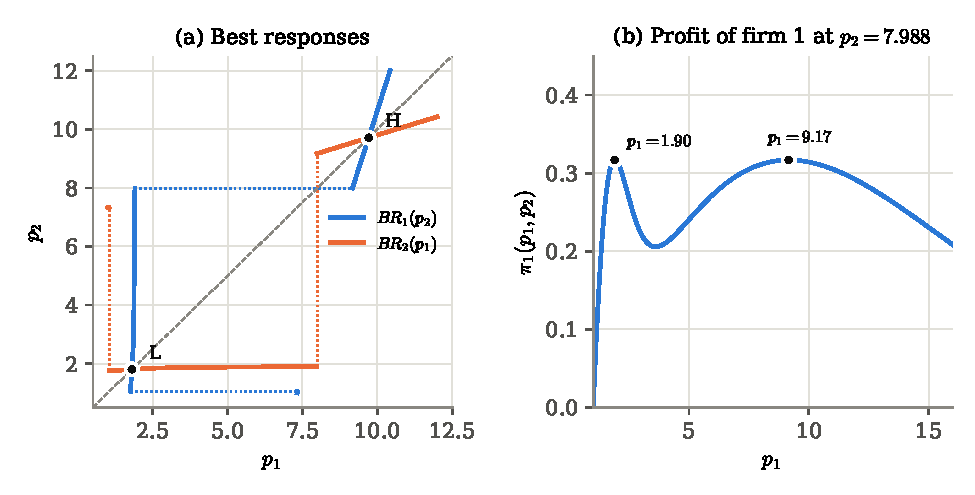
\includegraphics[width=\textwidth]{figures/ch04/multiple_equilibria.pdf}
  \caption{Two equilibria in the two-segment logit duopoly of \cref{ex:04-multiple-eq}. Panel (a): best responses
  $BR_1(p_2)$ and $BR_2(p_1)$, with dotted segments marking the jumps. They cross on the 45-degree line at the
  mass-market equilibrium $L$ ($p^* = 1.804$) and at the niche equilibrium $H$ ($p^* = 9.711$). Panel (b): firm 1's
  profit as a function of its own price when $p_2 = 7.988$. Two local maxima, at $p_1 = 1.904$ and $p_1 = 9.168$,
  give the same profit, so profit is not quasi-concave. Computed with
  \texttt{figures/ch04/src/multiple\_equilibria.py}.}
  \label{fig:04-multiple-eq}
\end{figure}

The example violates the Caplin-Nalebuff conditions in an instructive way. Dividing utility by $\alpha_h$, a consumer
of segment $h$ buys $j$ when $\frac{\delta + \epsilon_{ij} - \epsilon_{i0}}{\alpha_h} - p_j$ is largest. A1 holds
with $g(z) = z$ and money-metric types $\nu_{ij} = \frac{\delta + \epsilon_{ij} - \epsilon_{i0}}{\alpha_h}$. Within a
segment, the vector $(\nu_{i1}, \nu_{i2})$ is a linear transformation of independent extreme value shocks and has a
log-concave density. Across segments, its density is a mixture of a component concentrated near
$\frac{\delta}{\alpha_A} = 1.5$ and a component spread around $\frac{\delta}{\alpha_B} = 15$. The mixture is bimodal.
It is not even quasi-concave, so A2 fails, and profit inherits two peaks from the two groups of consumers.

\casehead{Consequences for empirical work}
Multiplicity does not affect the estimation methods of this chapter. At the estimation stage, prices are data. We
evaluate the first-order conditions at observed prices and invert them for marginal costs as in \eqref{eq:04-mc-recover},
so we never solve for an equilibrium. Whichever equilibrium generated the data, the first-order conditions hold at
the observed prices. In games of entry and in dynamic games, by contrast, multiplicity complicates estimation
itself.

Counterfactuals are different. A merger simulation or a policy experiment must solve for new prices, and with
several solutions the researcher must choose among them. Three selection rules are common. The first starts the
solver at the status quo prices. Merger simulations usually iterate from pre-merger prices, which selects the
equilibrium in whose basin of attraction the status quo lies. The \emph{basin of attraction} of an equilibrium is
the set of starting points from which the iteration converges to it. The second picks the equilibrium the firms prefer,
which here is $H$. The third requires stability under best-response dynamics. In \cref{ex:04-multiple-eq} both
equilibria are stable. Simultaneous best-response iteration from a symmetric start converges to $L$ for starting
prices below 7.988 and to $H$ above. From an asymmetric start such as $(2, 12)$, however, it cycles between
$(1.804, 9.711)$ and $(9.711, 1.804)$, although neither point is an equilibrium. Alternating best responses avoid
the cycle. Stability depends on the adjustment process, and a careful counterfactual reports how its answer depends
on the selection rule (\cref{sec:04-counterfactuals}).

These problems explain part of the popularity of demand systems with known uniqueness results, such as the logit and
CES with multi-product firms (\cref{thm:04-logit-unique} and \citealp{NockeSchutz2018}). For richer systems, the checks
listed at the end of \cref{sec:04-uniqueness} are the practical safeguard. They cannot prove uniqueness, but they can
reveal multiplicity when it is present.

\section{Using the supply side: costs, conduct and counterfactuals}\label{sec:04-supply}

\Cref{sec:04-bertrand,sec:04-diversion,sec:04-existence} characterized the pricing equilibrium and the conditions
under which it exists and is unique. We now put the pricing rule to work. The first-order conditions
\eqref{eq:04-foc-matrix} tie together four objects: the demand system and its
derivatives, the ownership matrix, prices and marginal costs. Given any three of them, the conditions restrict
the fourth. This section uses them in three directions. With estimated demand, observed prices and an assumed
ownership structure, they recover marginal costs without any cost data (\cref{sec:04-mc}). With demand and
independent information on margins, they let us compare models of conduct (\cref{sec:04-conduct}). With
demand, recovered costs and a changed environment, they predict the new equilibrium
(\cref{sec:04-counterfactuals,sec:04-comparative}). We begin with the reasons for modeling supply at all.

\subsection{Why model supply when we estimate demand?}\label{sec:04-supply-why}

Write the markup equation \eqref{eq:04-markup} product by product, and let marginal cost depend on observed
\emph{cost shifters} $w_j$ (variables that move cost but not utility) and an unobserved cost shock $\omega_j$:
\begin{equation}\label{eq:04-price-decomp}
p_j = mc_j(w_j, \omega_j) + m_j(p, x, \xi;\, \theta_d, \Omega),
\qquad m = -\big(\Omega \odot \Delta^\top\big)^{-1} q .
\end{equation}
Here $\theta_d$ collects the demand parameters, $x$ and $\xi$ stack the observed and unobserved characteristics
of all products, and $m_j$ is the $j$th element of the markup vector $m$. Equation \eqref{eq:04-price-decomp} is
a model of price. A product's price moves with its own cost and with every determinant of its markup, including
the characteristics and prices of all other products. Three reasons to model supply follow from it.

\casehead{Prices are endogenous, and supply tells us which instruments are valid}
Take the logit demand of \cref{sec:04-bertrand-logit}, with mean utility $\delta_j = x_j\beta - \alpha p_j +
\xi_j$. Firms observe the unobserved quality $\xi_j$ when they set prices, so $p_j$ responds to it. For a
single-product firm the pricing condition is $p_j = mc_j + \frac{1}{\alpha(1 - s_j)}$ by
\cref{prop:04-logit-markup}. Hold rivals' prices fixed and define
\begin{equation*}
F(p_j, \xi_j) \equiv p_j - mc_j - \frac{1}{\alpha(1 - s_j)} = 0 .
\end{equation*}
The logit derivatives \eqref{eq:04-logit-derivs} give $\frac{\partial s_j}{\partial p_j} = -\alpha s_j(1 - s_j)$,
and the same algebra gives $\frac{\partial s_j}{\partial \xi_j} = s_j(1 - s_j)$. Differentiating $F$,
\begin{align*}
\frac{\partial F}{\partial p_j} &= 1 - \frac{1}{\alpha(1 - s_j)^2}\,\frac{\partial s_j}{\partial p_j}
  = 1 + \frac{s_j}{1 - s_j} = \frac{1}{1 - s_j}, \\
\frac{\partial F}{\partial \xi_j} &= -\frac{1}{\alpha(1 - s_j)^2}\,\frac{\partial s_j}{\partial \xi_j}
  = -\frac{s_j}{\alpha(1 - s_j)} .
\end{align*}
By the implicit function theorem (\cref{app:math}),
\begin{equation}\label{eq:04-dp-dxi}
\frac{d p_j}{d \xi_j} = -\frac{\frac{\partial F}{\partial \xi_j}}{\frac{\partial F}{\partial p_j}}
= \frac{s_j}{\alpha(1 - s_j)}\,(1 - s_j) = \frac{s_j}{\alpha} > 0 .
\end{equation}
Products with high unobserved quality carry high prices. In the logit estimating equation $\ln s_j - \ln s_0 =
x_j\beta - \alpha p_j + \xi_j$ of \cref{ch:logit}, the regressor $p_j$ is therefore positively correlated with the
error $\xi_j$. Least squares biases the price coefficient $-\alpha$ toward zero, and estimated demand looks too
inelastic.

The price equation also tells us which variables can serve as instruments. A valid instrument moves $p_j$ and is
uncorrelated with $\xi_j$. By \eqref{eq:04-price-decomp} three groups of variables move prices. Cost shifters
$w_j$ move $mc_j$ and are excluded from utility. Characteristics of other products move $m_j$ through shares and
diversion ratios, and they are excluded from the utility of product $j$. Changes in ownership move $m_j$ through
$\Omega$. \citet[eq.~(4.1)]{BerryLevinsohnPakes1995} state the identifying assumption as $\E[\xi_j \mid z] =
\E[\omega_j \mid z] = 0$, where $z$ stacks the characteristics and cost shifters of all products.
\Cref{ch:logit,ch:blp} develop these instruments, and \cref{sec:06-charinst} explains why instruments built from
characteristics fail when firms choose characteristics with knowledge of $\xi_j$.

\casehead{The pricing equation adds information about demand}
Suppose we specify $mc_j = w_j\gamma + \omega_j$ and fix $\Omega$. For any candidate value of $\theta_d$ we can
compute the markups $m(\theta_d)$ at observed prices and quantities, and with them the implied cost shock
\begin{equation*}
\omega_j(\theta_d, \gamma) = p_j - m_j(\theta_d) - w_j\gamma .
\end{equation*}
Moment conditions $\E[z_j\,\omega_j(\theta_d, \gamma)] = 0$ then restrict $\theta_d$ as well as $\gamma$. A price
coefficient that is too small in absolute value, for example, implies markups that are too large. The implied
costs are then too low exactly where markups are high, and they become correlated with instruments that shift
markups. \citet{BerryLevinsohnPakes1995} estimate demand and the pricing equation jointly for this reason
(\cref{ch:blp}).

\casehead{Markups, costs and counterfactuals require a model of price setting}
Demand alone yields elasticities and diversion ratios. Markups require a model of how prices are set, and so do
the marginal costs inferred from them. Every counterfactual that changes prices, such as a merger, a new product
or a tax, requires solving for a new equilibrium.

These reasons come with a trade-off. Demand can usually be estimated without specifying supply in full.
Instruments motivated by supply, such as cost shifters, remain valid whatever the exact model of conduct, as long
as they are excluded from utility and uncorrelated with $\xi_j$. Adding the pricing equation brings more
information and more assumptions. If conduct or the cost function is misspecified, joint estimation transmits the
error into the demand estimates. The researcher therefore trades efficiency against robustness. Counterfactuals
need a model of supply in any case, so the assumptions return at that stage even when estimation avoids them.

\subsection{Recovering marginal costs}\label{sec:04-mc}

Suppose demand has been estimated, with parameter estimate $\hat\theta_d$, and that we observe prices $p$ and
quantities $q$ in a market. The demand Jacobian $\Delta(p; \hat\theta_d)$ can then be evaluated at the observed
prices. We rearrange \eqref{eq:04-foc-matrix} in two steps:
\begin{align*}
\big(\Omega \odot \Delta^\top\big)(p - mc) &= -q, \\
p - mc &= -\big(\Omega \odot \Delta^\top\big)^{-1} q .
\end{align*}
Solving for marginal cost gives the \emph{implied} (or recovered) marginal cost
\begin{equation}\label{eq:04-mc-recover}
\widehat{mc} = p + \big(\Omega \odot \Delta(p; \hat\theta_d)^\top\big)^{-1} q .
\end{equation}
\Cref{prop:04-markup-positive} guarantees that the inverse exists and that the implied markups are positive
whenever some of every product's lost sales go to the outside good. With market size $M$, $q = Ms$ and
$\Delta = M\Delta^s$, so the same formula holds with shares and share derivatives. The computation is done market
by market, and it uses no cost data.

\begin{remark}[What cost recovery assumes]\label{rem:04-mc-assumptions}
Formula \eqref{eq:04-mc-recover} rests on four assumptions. (i) The demand model is correctly specified and
$\hat\theta_d$ is consistent. (ii) Observed prices satisfy the first-order conditions of a static
simultaneous-move pricing game, with interior prices. (iii) The matrix $\Omega$ describes conduct correctly.
(iv) Marginal cost is constant, or the recovered value is read as marginal cost at the observed output. The
formula does not require the equilibrium to be unique. \citet[fn.~12]{BerryLevinsohnPakes1995} note that ``none
of the properties of the estimates require uniqueness of equilibrium.'' Uniqueness matters only at the
counterfactual stage (\cref{sec:04-counterfactuals}).
\end{remark}

With logit demand the inversion has a closed form. By \cref{prop:04-logit-markup} every product of firm $f$
carries the markup $\frac{1}{\alpha(1 - S_f)}$, where $S_f$ is the firm's combined share. Hence
\begin{equation}\label{eq:04-mc-logit}
\widehat{mc}_j = p_j - \frac{1}{\hat\alpha\,\big(1 - S_{f(j)}\big)} .
\end{equation}
Within a firm, differences in recovered costs equal differences in prices. Across firms, a product of a firm with
a larger combined share is assigned a larger markup, and so a lower cost at a given price.

\begin{example}[Cost recovery under three models of conduct]\label{ex:04-mc-recovery}
Treat the multi-product equilibrium (M) of \cref{ex:04-logit25} as data. Its prices range from 0.744 to 1.852,
and the true marginal costs range from 0.164 to 1.236. We apply \eqref{eq:04-mc-recover} with the true $\alpha
= 2$ and three ownership matrices.
\begin{enumerate}
  \item With the true owners, the recovered costs equal the true costs up to rounding error.
  \item If we wrongly assume single-product firms ($\Omega = I_{25}$), the implied markups are
  $\frac{1}{\alpha(1 - s_j)}$, between 0.502 and 0.568. The recovered costs then exceed the true costs by 0.014 to
  0.168, by 0.098 on average, against a mean true cost of 0.767.
  \item If we assume that one owner sets all 25 prices ($\Omega = \mathbf{1}\mathbf{1}^\top$), every markup equals
  $\frac{1}{\alpha s_0} = \frac{1}{2 \times 0.1601} = 3.12$. All 25 recovered costs are negative, with mean $-1.74$.
\end{enumerate}
Assuming too little internalization overstates costs, and assuming too much understates them. The third case
shows that implausible implied costs can reject a model of conduct outright.
\end{example}

\casehead{Why the New Empirical IO avoids accounting costs}
Formula \eqref{eq:04-mc-recover} is the answer of the New Empirical Industrial Organization to the unreliability
of accounting cost data \citep{Bresnahan1989}, discussed in \cref{ch:intro,ch:conduct}. Accounting data have
four problems for our purpose. First, they report average (variable) cost, which differs from marginal cost
unless returns to scale are constant. Second, multi-product firms share plants, distribution and advertising, and
accountants allocate these common costs across products by conventions without economic content. Third,
accounting depreciation follows tax and reporting rules, and the opportunity cost of capital and of owned inputs
is missing \citep{FisherMcGowan1983}. Fourth, the data are reported by firm or division, not by product and
market. The structural approach trades these measurement problems for dependence on the demand model and on the
assumed conduct. Accounting data then become a check on the model. \citet[p.~333]{Nevo2001}, for example, uses
accounting margins only as a crude benchmark. He treats Census margins, built from average variable costs, as an
upper bound on price-cost margins.

\casehead{The cost equation}
We often want to know what determines the recovered costs: input prices, returns to scale, the cost of
characteristics, or the savings from a merger. The standard specification projects marginal cost on cost
shifters:
\begin{equation}\label{eq:04-cost-eq}
mc_j = w_j\gamma + \omega_j
\qquad\text{or}\qquad
\ln mc_j = w_j\gamma + \omega_j ,
\end{equation}
where $w_j$ is a row vector of observed cost shifters and $\omega_j$ is the unobserved cost shock.
\citet[eq.~(3.1)]{BerryLevinsohnPakes1995} use the log form. Their $w_j$ contains product characteristics, and they
note that $\omega_j$ may be correlated with $\xi_j$ because larger cars, or cars with higher unobserved quality,
may cost more to produce (p.~853).

\citet{BerryLevinsohnPakes1995} write the first-order conditions with the opposite sign convention. Their $J
\times J$ matrix has element $(j, r)$ equal to $-\frac{\partial s_r}{\partial p_j}$ when products $r$ and $j$ have
the same owner and zero otherwise (their eq.~3.4). In our notation it is $-(\Omega \odot \Delta^{s\top})$. Their
first-order conditions read $s - \Delta^{\mathrm{BLP}}(p - mc) = 0$, and their markup is
\begin{equation}\label{eq:04-blp-markup}
b(p, x, \xi; \theta) = \big(\Delta^{\mathrm{BLP}}\big)^{-1}s = -\big(\Omega \odot \Delta^{s\top}\big)^{-1}s
\end{equation}
(their eq.~3.5). Substituting into \eqref{eq:04-cost-eq} gives the \emph{pricing equation} that is taken to the
data,
\begin{equation}\label{eq:04-cost-est}
p_j - b_j(\hat\theta_d) = w_j\gamma + \omega_j
\qquad\text{or}\qquad
\ln\big(p_j - b_j(\hat\theta_d)\big) = w_j\gamma + \omega_j ,
\end{equation}
where the log version is their eq.~(3.6). The left side is the recovered marginal cost $\widehat{mc}_j$.

\casehead{Why the error enters additively}
Because $\omega_j$ enters \eqref{eq:04-cost-est} additively, we can solve for it at any parameter value:
$\omega_j(\theta_d, \gamma) = \widehat{mc}_j(\theta_d) - w_j\gamma$. Given instruments $z_j$, the moment
conditions
\begin{equation}\label{eq:04-supply-moment}
\E\big[z_j^\top\,\omega_j(\theta_{d0}, \gamma_0)\big] = 0
\end{equation}
are linear in $\gamma$ for fixed $\theta_d$, so $\gamma$ is estimated by linear instrumental variables. If the
cost shock entered nonseparably, for example as $mc_j = c(w_j, \omega_j)$ with $c$ not invertible in $\omega_j$,
we could not compute the residual and these moments would be unavailable. Additivity is what makes the
econometrics simple.

\casehead{When the cost equation needs instruments}
With $\theta_d$ known and constant marginal cost, \eqref{eq:04-cost-est} is a regression of cost on its
determinants, and least squares is consistent if $\E[\omega_j \mid w_j] = 0$. Three features of applications
break this condition. First, $w_j$ often includes output, as in $\ln mc_j = w_j\gamma + \gamma_q\ln q_j + \omega_j$,
to allow for returns to scale. A high $\omega_j$ raises $p_j$ and lowers $q_j$, so $q_j$ is correlated with the
error. Second, the characteristics in $w_j$ may have been chosen with knowledge of $\omega_j$. Third, tests of
conduct place the markup on the right side with a free coefficient $\vartheta$, as in $p_j = w_j\gamma +
\vartheta\, b_j + \omega_j$. Here \citet[p.~854]{BerryLevinsohnPakes1995} point out that ``since $p$ is a function of $\omega$,
$b(p, x, \xi; \theta)$ is a function of $\omega$'' and cannot be assumed uncorrelated with it. In each case we
need excluded instruments, such as demand shifters and characteristics of rival products, which move output or
markups but are mean independent of $\omega_j$.

\casehead{The recovered cost is a generated regressand}
The left side of \eqref{eq:04-cost-est} depends on $\hat\theta_d$. Consistency of $\hat\gamma$ follows from
consistency of $\hat\theta_d$. The usual standard errors are wrong, however, because they ignore the estimation
error in $\hat\theta_d$. With least squares on the stacked cost shifters $\mathcal{W}$, a first-order expansion gives
\begin{equation}\label{eq:04-generated}
\hat\gamma - \gamma_0 \approx \big(\mathcal{W}^\top \mathcal{W}\big)^{-1}\mathcal{W}^\top\Big[\omega + \frac{\partial\,\widehat{mc}(\theta_{d0})}
{\partial\theta_d^\top}\big(\hat\theta_d - \theta_{d0}\big)\Big].
\end{equation}
The second term adds variance, and it is correlated across all products and markets that share $\hat\theta_d$.
There are two remedies. We can stack the demand and supply moments into one GMM problem and use its joint
asymptotic variance (\cref{ch:blp,app:econometrics}). Or we can bootstrap, resampling markets and re-estimating
demand in each replication.

\begin{example}[Cost regressions under three models of conduct]\label{ex:04-cost-regression}
Continue \cref{ex:04-mc-recovery}. The true costs satisfy $mc_j = x_j\gamma + \omega_j$ with $\gamma = (0.2,
0.25, 0.3)$, where $x_j$ contains a constant, a continuous characteristic and a binary characteristic. A least
squares regression of the true costs on $x_j$ gives $\hat\gamma = (0.182, 0.250, 0.310)$, with standard errors
$(0.025, 0.010, 0.020)$. Costs recovered with the true owners give the same estimates. Costs recovered under
single-product conduct give $(0.303, 0.239, 0.305)$. Costs recovered under one owner give $(-2.301, 0.235, 0.316)$.
The conduct error loads almost entirely on the intercept here, because logit markups vary little with the
characteristics. In richer demand models markup errors are correlated with characteristics, and they bias the
slopes too.
\end{example}

\subsection{Conduct and the ownership matrix}\label{sec:04-conduct}

Bertrand-Nash pricing with the true owners is one model of conduct. We now embed it in a family of models
indexed by profit weights. This makes conduct comparable with the conduct parameter $\theta$ of
\cref{ch:conduct}.

\begin{definition}[Profit weights and the generalized ownership matrix]\label{def:04-profit-weights}
Let $\kappa_{fg} \ge 0$ be the weight that firm $f$ places on the profit of firm $g$, with $\kappa_{ff} = 1$.
Firm $f$ chooses the prices of its products to maximize
\begin{equation}\label{eq:04-kappa-objective}
\pi_f + \sum_{g \neq f}\kappa_{fg}\,\pi_g ,
\end{equation}
taking the prices of other firms as given. The \emph{generalized ownership matrix} $\Omega(\kappa)$ has elements
$\Omega(\kappa)_{jk} = \kappa_{f(j)f(k)}$, where $f(j)$ is the owner of product $j$.
\end{definition}

The symbol $\kappa$ denotes profit weights throughout this chapter. \Cref{ch:conduct} uses the same letter for a
different object.

\begin{lemma}[First-order conditions with profit weights]\label{lem:04-kappa-foc}
With profit weights $\kappa$, the first-order conditions of all firms are
\begin{equation}\label{eq:04-foc-kappa}
q + \big(\Omega(\kappa) \odot \Delta^\top\big)(p - mc) = 0 .
\end{equation}
\end{lemma}

\begin{proof}
Firm $g$'s profit is $\pi_g = \sum_{k \in \mathcal{J}_g}(p_k - mc_k)q_k(p)$ with constant marginal costs. Take
$j \in \mathcal{J}_f$ and differentiate \eqref{eq:04-kappa-objective} with respect to $p_j$. The own-profit term
gives $q_j + \sum_{k \in \mathcal{J}_f}(p_k - mc_k)\frac{\partial q_k}{\partial p_j}$, as in
\eqref{eq:04-foc-scalar}. The term for firm $g \neq f$ gives $\kappa_{fg}\sum_{k \in \mathcal{J}_g}(p_k -
mc_k)\frac{\partial q_k}{\partial p_j}$, because $p_j$ enters $\pi_g$ only through the quantities. Adding the terms
and using $\kappa_{ff} = 1$,
\begin{equation*}
q_j + \sum_{k = 1}^{J}\kappa_{f(j)f(k)}\,(p_k - mc_k)\frac{\partial q_k}{\partial p_j} = 0 .
\end{equation*}
The coefficient of $(p_k - mc_k)$ is $\Omega(\kappa)_{jk}\Delta_{kj} = (\Omega(\kappa) \odot \Delta^\top)_{jk}$, so
stacking over $j$ gives \eqref{eq:04-foc-kappa}.
\end{proof}

Row $j$ of $\Omega(\kappa)$ describes the objective of the firm that sets $p_j$. The matrix need not be
symmetric, because $\kappa_{fg}$ and $\kappa_{gf}$ can differ. Cost recovery \eqref{eq:04-mc-recover},
counterfactuals and pass-through all go through with $\Omega(\kappa)$ in place of $\Omega$. Four cases are
standard.
\begin{enumerate}
  \item \emph{Nash pricing} sets $\kappa_{fg} = 0$ for $f \neq g$, so $\Omega(\kappa) = \Omega$.
  \item \emph{Full collusion}, or joint profit maximization, sets $\kappa_{fg} = 1$ for all $f$ and $g$, so
  $\Omega(\kappa) = \mathbf{1}\mathbf{1}^\top$. Whether such conduct can be sustained is the subject of
  \cref{ch:collusion-theory}.
  \item A \emph{merger} of firms $f$ and $g$ sets $\kappa_{fg} = \kappa_{gf} = 1$ and leaves the other weights at
  zero.
  \item \emph{Partial internalization} has weights strictly between zero and one. Joint ventures and moderate
  common ownership produce such weights.
\end{enumerate}
These cases span the range $\kappa_{fg} \in [0, 1]$, from Nash pricing to joint profit maximization. Many conduct
models restrict the weights to this range. The restriction is an additional assumption, and the common-ownership
weights below need not satisfy it.

\casehead{Common ownership}
\citet{OBrienSalop2000} derive profit weights from ownership stakes. Let investors $h = 1, \dots, H$ hold
cash-flow shares $\lambda_{gh}$ in firm $g$, and let $\eta_{fh}$ be investor $h$'s share of control over firm
$f$. (The symbols $\lambda$, $\eta$, $h$ and $H$ are local to this paragraph.) Suppose the manager of firm $f$
maximizes the control-weighted sum of its investors' portfolio profits:
\begin{equation*}
\sum_{h = 1}^{H}\eta_{fh}\sum_{g = 1}^{F}\lambda_{gh}\,\pi_g
= \sum_{g = 1}^{F}\Big(\sum_{h = 1}^{H}\eta_{fh}\lambda_{gh}\Big)\pi_g .
\end{equation*}
Dividing by the coefficient on $\pi_f$ leaves the maximizer unchanged and gives the form
\eqref{eq:04-kappa-objective} with
\begin{equation}\label{eq:04-obrien-salop}
\kappa_{fg} = \frac{\sum_{h}\eta_{fh}\lambda_{gh}}{\sum_{h}\eta_{fh}\lambda_{fh}} ,
\end{equation}
provided that the investors who control $f$ hold some cash-flow stake in $f$, so that the denominator is positive.
The weight is large when the investors who control $f$ own large cash-flow stakes in $g$. Nothing bounds it by
one. If the sole controlling investor of $f$ holds 10 percent of $f$ and 90 percent of $g$, then
$\kappa_{fg} = \frac{0.9}{0.1} = 9$. The manager of $f$ then values a dollar of $g$'s profit at nine dollars of
its own.
\citet{BackusConlonSinkinson2021} compute such weights for the ready-to-eat cereal industry and ask whether
pricing reflects them.

\casehead{Joint ventures}
\citet{MillerWeinberg2017} study the 2008 joint venture that combined the US operations of SABMiller and Molson
Coors. The Department of Justice approved the transaction on June 5, 2008, on the ground that efficiencies in
brewing would outweigh any adverse competitive effect \citep[p.~241, n.~161]{AskerNocke2021}. Almost immediately after
clearance, the prices of 12-packs of Miller Lite, Bud Light and Coors Light rose by about 8 percent. The imported
flagship brands Corona Extra and Heineken show little persistent change \citep[p.~242]{AskerNocke2021}. Miller and
Weinberg's demand system is a random coefficients nested logit. On the supply side, a weight $\kappa \in [0, 1]$ captures coordination between
brands that are not jointly owned. It enters the ownership matrix of the standard first-order conditions and is
estimated. A weight of zero is Nash pricing, and a weight of one is joint profit maximization. The estimate rejects
unilateral price competition \citep[p.~242, n.~164]{AskerNocke2021}. In their specification the weight applies to
pairs of products of Anheuser-Busch InBev (ABI) and MillerCoors in the periods after the joint venture
\citep[Section~5.1, p.~1779]{MillerWeinberg2017}. \Cref{ch:mergers} treats the application.

\begin{remark}[Profit weights and the conduct parameter]\label{rem:04-kappa-theta}
Profit weights give the conduct parameter of \cref{ch:conduct} a structural reading. Let $N$ symmetric Cournot
firms with constant marginal cost $c$ each maximize $\pi_i + \kappa\sum_{l \neq i}\pi_l$, with $\pi_l = (P(Q) -
c)q_l$. The first-order condition of firm $i$ is
\begin{equation*}
P(Q) - c + P'(Q)\Big(q_i + \kappa\sum_{l \neq i}q_l\Big) = 0 .
\end{equation*}
At a symmetric equilibrium $q_i = \frac{Q}{N}$, so $q_i + \kappa\sum_{l \neq i}q_l = \frac{1 + \kappa(N - 1)}{N}Q$
and
\begin{equation*}
P(Q) = c - \frac{1 + \kappa(N - 1)}{N}\,Q\,P'(Q) .
\end{equation*}
This is the supply relation \eqref{eq:03-supply-relation} with $\theta = \frac{1 + \kappa(N - 1)}{N}$. Nash
behavior ($\kappa = 0$) gives the Cournot value $\theta = \frac{1}{N}$, and full collusion ($\kappa = 1$) gives
$\theta = 1$. With differentiated products, however, conduct is a matrix. We therefore compare a short menu of
ownership matrices, or estimate a low-dimensional $\kappa$, rather than a free parameter for every pair of
products.
\end{remark}

\casehead{Testing conduct}
Two ownership matrices $\Omega^A$ and $\Omega^B$ imply two markup vectors and two vectors of recovered costs. There
are four main ways to choose between them. First, implied costs may be implausible, as the negative costs of
\cref{ex:04-mc-recovery} are. Second, implied margins can be compared with independent measures of margins, as in
\citet{Nevo2001} below. Third, nonnested tests compare the fit of the full models, as in the 1955 automobile
price war studied by \citet{Bresnahan1987} (\cref{sec:06-bresnahan}). A \emph{nonnested test} compares two models,
neither of which is a special case of the other. Fourth, under the true model the implied
cost shock is mean independent of excluded instruments, while under a false model it generally is not.
\citet[Section~6, p.~1776]{BerryHaile2014} give a formal foundation, in a much more general setting, to the
intuition of \citet{Bresnahan1982}, discussed in \cref{sec:03-rotation}. Their results allow product differentiation and do not require rotations of
demand. Variation in the number of competing firms, the set of competing goods, or the characteristics or costs of
competitors can discriminate between models of conduct (p.~1779).

\casehead{An application: margins in ready-to-eat cereal}
\citet{Nevo2001} estimates a random coefficients demand system for 25 brands of ready-to-eat cereal and uses the
pricing equation to decompose margins (\cref{ch:blp} gives the full case study). His supply side writes the
first-order conditions as $s(p) - \Omega(p - mc) = 0$, where $\Omega_{jr} = \Omega^*_{jr}S_{jr}$, $S_{jr} =
-\frac{\partial s_r}{\partial p_j}$, and $\Omega^*$ is the ownership matrix. This is the convention of
\citet{BerryLevinsohnPakes1995}. The implied markups are (his eq.~1, p.~313)
\begin{equation}\label{eq:04-nevo-markup}
p - mc = \Omega^{-1}s(p) .
\end{equation}
Nevo evaluates \eqref{eq:04-nevo-markup} under three structures. With \emph{single-product firms}, each brand is
priced by an agent who cares only about that brand, and margins reflect product differentiation alone. With the
\emph{current ownership} of the brands by multi-product firms, margins also reflect the internalization of
substitution among a firm's brands. With \emph{joint ownership} of all brands, margins are those of a monopolist
or of a perfect cartel. The margins of the three structures define a decomposition,
\begin{equation}\label{eq:04-nevo-decomp}
m^{\mathrm{joint}} = \underbrace{m^{\mathrm{single}}}_{\text{differentiation}}
+ \underbrace{\big(m^{\mathrm{current}} - m^{\mathrm{single}}\big)}_{\text{portfolio effect}}
+ \underbrace{\big(m^{\mathrm{joint}} - m^{\mathrm{current}}\big)}_{\text{collusion effect}} .
\end{equation}
Each term is nonnegative product by product when goods are substitutes (\cref{prop:08-nevo-ownership}).

The three structures imply very different margins. With the full random coefficients model, the median margin $\frac{p - mc}{p}$ over
27,862 brand-city-quarter observations is 35.8 percent with single-product firms. It is 42.2 percent under current
ownership and 72.6 percent under joint ownership of the 25 brands \citep[Table~VIII]{Nevo2001}. Product
differentiation thus accounts for most of the predicted margin, and the portfolio effect adds 6.4 percentage
points. Joint profit maximization would add 30.4 points more. Nevo compares these predictions with a gross retail
margin of 46.0 percent from accounting sources. The price gap between national brands and private labels gives a
lower bound of about 31 percent (p.~333). He rejects joint profit maximization of the 25 brands, whose 95
percent confidence interval runs from 62.2 to 97.2 percent. He cannot reject multi-product Nash pricing, whose
interval runs from 29.1 to 55.8 percent (p.~334).

The logit version of the same exercise illustrates why the demand model matters for conduct. With logit demand,
the median margins are 33.6, 35.8 and 41.9 percent under the three structures, and 54.0 percent if all brands in
the market are priced jointly \citep[Table~VIII]{Nevo2001}. The mean price sensitivity of the full model is close
to the logit price coefficient. The gap between the models widens from single-product to joint ownership, because
the full model captures cross-price substitution better (p.~332). By \cref{prop:04-logit-markup}, logit markups
depend on ownership only through combined shares. When those shares are small, as they are when the outside good is
large, internalizing rival brands changes logit margins little.
Nevo notes that with the logit estimates one cannot reject full collusion over all products, and he attributes
this to the strong assumptions of the logit rather than to conduct (p.~335). A demand model that hardly
distinguishes conduct structures cannot test them. \Cref{tab:08-nevo-margins} in \cref{ch:blp} reproduces the full
table.

\subsection{Counterfactual analysis}\label{sec:04-counterfactuals}

A counterfactual asks what would happen under conditions never observed: a merger that has not occurred, a
product not yet launched, a tax not yet levied. Answering it requires a model whose primitives remain valid under
the new conditions.

\begin{definition}[Structural model and counterfactual]\label{def:04-structural}
A model is \emph{structural} with respect to a change in the environment if its primitives do not change when the
environment changes. Here the primitives are the demand parameters and unobserved qualities $\xi$, the cost
function and cost shocks $\omega$, and the rule of conduct. A
\emph{counterfactual} is the equilibrium of the model after one element of the environment is changed, with all
other primitives held at their estimated values.
\end{definition}

\begin{remark}[The counterfactual algorithm]\label{rem:04-algorithms}
A static counterfactual in a differentiated-products market proceeds in five steps.
\begin{enumerate}
  \item \emph{Estimate demand} from data on the status quo, with instruments for price (\cref{ch:logit,ch:blp}).
  Recover $\hat\xi$ along with $\hat\theta_d$.
  \item \emph{Recover marginal costs} at the observed prices and quantities from \eqref{eq:04-mc-recover}, using
  the status quo ownership matrix $\Omega^0$. Optionally estimate the cost equation \eqref{eq:04-cost-eq} and
  recover $\hat\omega$.
  \item \emph{Change the environment.} A merger, a divestiture or collusion changes the ownership matrix to
  $\Omega^1$ (for instance by setting to one the entries for pairs of products of the merging firms). Entry, exit or
  a new good changes the product set (\cref{ch:newgoods}). A new product needs characteristics $x_{J+1}$, an assumed
  quality $\xi_{J+1}$ (often zero, the mean of $\xi$) and a marginal cost from the cost equation. A tax, a tariff, an
  input-price change or a merger efficiency changes marginal costs: $mc_j + t_j$ for a specific tax $t_j$, and
  $(1 - E_j)mc_j$ for a proportional efficiency $E_j$, as in \eqref{eq:04-upp}.
  \item \emph{Solve for the new equilibrium}, that is, find $p^1$ with
  \begin{equation*}
  q(p^1) + \big(\Omega^1 \odot \Delta(p^1)^\top\big)\big(p^1 - mc^1\big) = 0 ,
  \end{equation*}
  using the demand model to evaluate $q(\cdot)$ and $\Delta(\cdot)$ at every trial price vector.
  \item \emph{Compute outcomes}, namely price and share changes, firms' profits, and consumer surplus from the
  demand model. With logit demand and market size $M$, the change in consumer surplus is $\frac{M}{\alpha}\ln\frac{\Phi^1}
  {\Phi^0}$, where $\Phi = 1 + \sum_k e^{\delta_k}$ (\cref{ch:logit}). With random coefficients the log-sum is
  integrated over consumers, each term divided by that consumer's $\alpha_i$.
\end{enumerate}
\end{remark}

Step 4 is the computational core. Four solution methods are common.
\begin{enumerate}
  \item \emph{Best-response iteration.} Each firm in turn maximizes its profit given the others' current prices,
  and the process repeats until prices stop changing. It converges when the best-response map is a contraction, as
  in the single-product logit (\cref{prop:04-logit-br}). With logit demand each step has the Lambert-W closed form
  of \cref{sec:04-bertrand-logit}.
  \item \emph{Markup iteration.} Iterate $p \leftarrow mc - (\Omega \odot \Delta(p)^\top)^{-1}q(p)$. The update is
  simple, but nothing guarantees convergence. Damped updates, which move prices only part of the way toward the
  right side, often help.
  \item \emph{Newton's method.} Write the stacked conditions as $G(p) = q(p) + (\Omega \odot \Delta(p)^\top)(p -
  mc)$ and iterate $p \leftarrow p - [\frac{\partial G}{\partial p^\top}]^{-1}G(p)$. Convergence is quadratic near
  the solution. The Jacobian involves second derivatives of demand, given in \eqref{eq:04-dGdp} below, and the
  method can wander when it starts far from the solution.
  \item \emph{The Morrow-Skerlos iteration.} For random coefficients logit demand with price coefficient $\alpha_i > 0$,
  split the share Jacobian as $\Delta^s(p) = -\Lambda(p) + \Gamma(p)$, with the diagonal matrix
  $\Lambda_{jj}(p) = \int\alpha_i s_{ij}(p)\,\dd F$ and the symmetric matrix $\Gamma_{jk}(p) = \int\alpha_i
  s_{ij}(p)s_{ik}(p)\,\dd F$. Here $s_{ij}$ is consumer $i$'s choice probability. The first-order conditions are
  then equivalent to the fixed point \citep{MorrowSkerlos2011}
  \begin{equation}\label{eq:04-ms}
  p - mc = \zeta(p) \equiv \Lambda(p)^{-1}\Big[s(p) + \big(\Omega \odot \Gamma(p)\big)(p - mc)\Big],
  \end{equation}
  which is iterated as $p \leftarrow mc + \zeta(p)$. The derivation is \cref{prop:08-ms} in \cref{ch:blp}. In the
  plain logit, $\Lambda = \alpha\diag(s)$ and $\Gamma = \alpha ss^\top$, so \eqref{eq:04-ms} becomes $m_j =
  \frac{1}{\alpha} + \sum_k\Omega_{jk}s_k m_k$. This is the fixed point of \cref{prop:04-logit-markup}.
\end{enumerate}

Whatever the method, convergence must be checked. We stop when the sup-norm change in prices falls below a tight
tolerance, such as $10^{-12}$, and then verify the first-order conditions directly. A residual in price units,
such as $\|\zeta(p) - (p - mc)\|_\infty$, is more informative than a residual in share units, which becomes small
at very high prices where every share is small. First-order conditions do not guarantee that each firm is at a
global maximum. Where profit may have several local maxima in own price (\cref{ex:04-multiple-eq}), we also
evaluate each firm's profit over a grid of unilateral deviations.

\casehead{Equilibrium selection}
\Cref{sec:04-multiple} showed that a counterfactual can have several equilibria even when estimation is
unaffected. An iterative solver selects the equilibrium in whose basin of attraction it starts, so the common
practice of starting from the status quo prices is itself a selection rule. A careful analysis restarts the solver
from many points and reports every equilibrium it finds. With logit demand and constant marginal costs the issue
does not arise, because the equilibrium is unique for every ownership structure (\cref{thm:04-logit-unique}).

\begin{example}[A simulated merger]\label{ex:04-merger-sim}
In the 25-product market of \cref{ex:04-logit25}, take the multi-product equilibrium (M) as the status quo and let
owners 3 and 4 merge. They hold 6 and 7 products with combined shares of 21.40 and 25.36 percent. We hold
marginal costs fixed and solve for the post-merger equilibrium with all four methods, starting from the
pre-merger prices. Best-response iteration and the Morrow-Skerlos iteration converge in 17 steps, markup iteration
needs 91 steps, and Newton's method with the analytic Jacobian \eqref{eq:04-dGdp} converges in 6 iterations. All
four reach the same prices, within
$5 \times 10^{-14}$. Five hundred random starting points lead to the same equilibrium, as
\cref{thm:04-logit-unique} implies. \Cref{tab:04-merger-sim} reports the results.
\end{example}

\begin{table}[htbp]
\centering
\caption{A simulated merger of owners 3 and 4 in the 25-product logit market}
\label{tab:04-merger-sim}
\footnotesize
\begin{tabular}{@{}lcccccccc@{}}
\toprule
 & & \multicolumn{2}{c}{Combined share (\%)} & \multicolumn{2}{c}{Markup} & Price & \multicolumn{2}{c}{Profit $\times 100$} \\
\cmidrule(lr){3-4}\cmidrule(lr){5-6}\cmidrule(l){8-9}
Owner & Products & Pre & Post & Pre & Post & change & Pre & Post \\
\midrule
\multicolumn{9}{@{}l}{\textit{Panel A. Owners}} \\
0 & 3 & 18.87 & 21.23 & 0.616 & 0.635 & 0.018 & 11.632 & 13.476 \\
1 & 3 & 4.67 & 5.41 & 0.524 & 0.529 & 0.004 & 2.449 & 2.857 \\
2 & 6 & 13.68 & 15.56 & 0.579 & 0.592 & 0.013 & 7.925 & 9.214 \\
3 (merging) & 6 & 21.40 & 17.25 & 0.636 & 0.821 & 0.185 & 13.616 & 14.167 \\
4 (merging) & 7 & 25.36 & 21.87 & 0.670 & 0.821 & 0.151 & 16.989 & 17.959 \\
\midrule
\multicolumn{9}{@{}l}{\textit{Panel B. Market}} \\
\multicolumn{3}{@{}l}{Outside share $s_0$} & 0.1601 & 0.1869 & & & & \\
\multicolumn{3}{@{}l}{Consumer surplus $\frac{1}{\alpha}\ln\Phi$} & 0.9159 & 0.8387 & & & & \\
\multicolumn{3}{@{}l}{Total profit} & 0.5261 & 0.5767 & & & & \\
\multicolumn{3}{@{}l}{Total surplus} & 1.4421 & 1.4154 & & & & \\
\multicolumn{3}{@{}l}{Share-weighted mean price} & 1.3553 & 1.4465 & & & & \\
\bottomrule
\end{tabular}

\vspace{3pt}
\begin{minipage}{0.97\textwidth}
\footnotesize Notes: Pre is the multi-product equilibrium (M) of \cref{tab:04-logit25}. Post is the equilibrium
after owners 3 and 4 merge, with marginal costs unchanged. Every product of an owner has the same markup and so
the same price change. Market size is one. Computed with \texttt{figures/ch04/src/supply\_examples.py}.
\end{minipage}
\end{table}

The merged firm prices all 13 of its products at the common markup 0.821. This equals $\frac{1}{\alpha(1 -
S)}$ at its post-merger combined share $S = 0.3912$, as \cref{prop:04-logit-markup} requires. The prices of
former owner 3 rise by 0.185 and those of former owner 4 by 0.151. Most of the increase is the merged firm's
unilateral response. If the merged firm best-responds to the unchanged pre-merger prices of its rivals, its markup
is 0.817. Rivals' price increases, between 0.004 and 0.018, add only 0.004 to it through strategic
complementarity.

The outsiders gain more than the merging parties. The merging parties' combined profit rises from 30.605 to
32.126 (times 100), while the rivals' combined profit rises from 22.006 to 25.547. The merged firm restricts its
own sales to raise price, and the rivals capture the diverted customers at higher prices. This free-riding
reappears in merger theory (\cref{ch:mergers}). Consumer surplus falls by 8.4 percent, the outside share rises
from 16.0 to 18.7 percent, and total surplus falls by 0.027.

How large would merger efficiencies need to be to leave consumers unharmed? With logit demand the answer has a
closed form. All prices stay at their pre-merger levels if and only if the merged firm's first-order condition
holds at the pre-merger prices. At those prices shares are unchanged, so the merged firm's markup must equal
$\frac{1}{\alpha(1 - S_3 - S_4)} = \frac{1}{2(1 - 0.4676)} = 0.939$. Marginal costs must therefore fall by $0.939
- 0.636 = 0.303$ for the products of owner 3 and by $0.939 - 0.670 = 0.269$ for those of owner 4. Re-solving the
equilibrium with these costs returns the pre-merger prices exactly. Such compensating cost reductions
\citep{Werden1996} are large here: 46 percent of owner 3's average marginal cost and 37 percent of owner 4's.

\subsection{Comparative statics and pass-through}\label{sec:04-comparative}

How do equilibrium prices respond to small changes in costs? The answer gives pass-through of taxes and input
prices, and it converts pricing pressure from a merger into price changes. We derive the general formula and then
evaluate it for logit demand.

\casehead{The general formula}
Write the stacked first-order conditions as a function of prices and marginal costs,
\begin{equation}\label{eq:04-G}
G(p; c) \equiv q(p) + \big(\Omega \odot \Delta(p)^\top\big)(p - c) = 0 ,
\end{equation}
with $c$ the vector of constant marginal costs. Row $j$ reads $G_j = q_j + \sum_k\Omega_{jk}\frac{\partial
q_k}{\partial p_j}(p_k - c_k)$. Differentiating with respect to $c_l$ gives
\begin{equation*}
\frac{\partial G_j}{\partial c_l} = -\Omega_{jl}\frac{\partial q_l}{\partial p_j},
\qquad\text{so}\qquad
\frac{\partial G}{\partial c^\top} = -\big(\Omega \odot \Delta^\top\big).
\end{equation*}
Differentiating with respect to $p_l$ gives three terms, one from $q_j$, one from the markup of product $l$, and
one from the dependence of the derivatives on prices:
\begin{equation*}
\frac{\partial G_j}{\partial p_l} = \frac{\partial q_j}{\partial p_l} + \Omega_{jl}\frac{\partial q_l}{\partial p_j}
+ \sum_k \Omega_{jk}(p_k - c_k)\frac{\partial^2 q_k}{\partial p_j\,\partial p_l} .
\end{equation*}
In matrix form,
\begin{equation}\label{eq:04-dGdp}
\frac{\partial G}{\partial p^\top} = \Delta + \Omega \odot \Delta^\top + H,
\qquad H_{jl} = \sum_k\Omega_{jk}\,m_k\,\frac{\partial^2 q_k}{\partial p_j\,\partial p_l} .
\end{equation}
If $\frac{\partial G}{\partial p^\top}$ is nonsingular at the equilibrium, the implicit function theorem
(\cref{app:math}) shows that equilibrium prices are locally a differentiable function of costs, with
\begin{equation}\label{eq:04-passthrough-matrix}
\frac{\partial p}{\partial c^\top} = -\Big[\frac{\partial G}{\partial p^\top}\Big]^{-1}\frac{\partial G}{\partial c^\top}
= \big[\Delta + \Omega \odot \Delta^\top + H\big]^{-1}\big(\Omega \odot \Delta^\top\big).
\end{equation}
For a single-product monopolist the matrices are scalars, and \eqref{eq:04-passthrough-matrix} reduces to
$\frac{q'}{2q' + (p - c)q''}$. This is the monopoly pass-through formula \eqref{eq:02-pt-monopoly} of
\cref{ch:theory}. The second derivatives in $H$ show that pass-through depends on the curvature of demand as
well as on its slope. A specific tax $t_j$ enters exactly like a cost, so \eqref{eq:04-passthrough-matrix} also gives
tax pass-through. The same formula holds with $\Omega(\kappa)$ in place of $\Omega$.

\casehead{Partial and full pass-through}
It helps to separate a firm's own response from the feedback through rivals' prices. For single-product firms,
let $BR_j(p_{-j}; c_j)$ be firm $j$'s best response, assumed differentiable. Define the \emph{partial pass-through}
$\rho^{\mathrm{p}}_j = \frac{\partial BR_j}{\partial c_j}$, which holds rivals' prices fixed, and the matrix $R$ of
best-response slopes, with $R_{jk} = \frac{\partial BR_j}{\partial p_k}$ for $k \neq j$ and $R_{jj} = 0$.

\begin{lemma}[Equilibrium pass-through from best responses]\label{lem:04-br-passthrough}
If $I - R$ is nonsingular at the equilibrium, then
\begin{equation}\label{eq:04-br-passthrough}
\frac{\partial p}{\partial c^\top} = (I - R)^{-1}\diag\big(\rho^{\mathrm{p}}\big).
\end{equation}
If moreover $\rho^{\mathrm{p}} > 0$, $R \geq 0$ element by element and every row sum of $R$ is below one, then
every element of $(I - R)^{-1} - I$ is nonnegative. Equilibrium own pass-through then weakly exceeds partial pass-through,
and a cost increase for one firm weakly raises every rival's price.
\end{lemma}

\begin{proof}
In equilibrium $p_j = BR_j(p_{-j}; c_j)$ for every $j$. Totally differentiating,
\begin{equation*}
dp_j = \sum_{k \neq j}R_{jk}\,dp_k + \rho^{\mathrm{p}}_j\,dc_j ,
\qquad\text{so}\qquad
(I - R)\,dp = \diag\big(\rho^{\mathrm{p}}\big)\,dc .
\end{equation*}
Multiplying by $(I - R)^{-1}$ gives \eqref{eq:04-br-passthrough}. If $R \geq 0$ with row sums below one, then
$\|R\|_\infty < 1$, so the Neumann series $(I - R)^{-1} = \sum_{n \geq 0}R^n$ converges. Every term is
nonnegative, so $(I - R)^{-1} - I = \sum_{n \geq 1}R^n \geq 0$. Since $\rho^{\mathrm{p}}_j > 0$, the diagonal of
$\frac{\partial p}{\partial c^\top}$ is at least $\rho^{\mathrm{p}}_j$ and the off-diagonal elements are nonnegative.
\end{proof}

\begin{proposition}[Partial pass-through with logit demand]\label{prop:04-passthrough}
Let demand be logit with constant marginal costs, and hold the prices of all other firms fixed.
\begin{enumerate}[label=(\roman*)]
  \item A single-product firm passes through the fraction $\frac{\partial p_j}{\partial c_j} = 1 - s_j$ of a cost
  increase.
  \item If the cost of product $j$ of a multi-product firm $f$ rises, then $\frac{\partial p_j}{\partial c_j} = 1 -
  s_j$, and the price of every other product $l \in \mathcal{J}_f$ falls, with $\frac{\partial p_l}{\partial c_j}
  = -s_j$.
  \item If the costs of all products of firm $f$ rise by the same amount $dc$, every price of firm $f$ rises by
  $(1 - S_f)\,dc$.
\end{enumerate}
\end{proposition}

\begin{proof}
By \cref{prop:04-logit-markup}, whatever its costs, firm $f$'s optimal prices satisfy $p_l = c_l + m_f$ for all
$l \in \mathcal{J}_f$, with a common markup that solves
\begin{equation}\label{eq:04-logit-foc-firm}
\alpha\, m_f\,(1 - S_f) = 1 .
\end{equation}
The firm's best response is the unique solution of this condition (\cref{sec:04-bertrand-logit}). After a change
in costs, the price changes are therefore $dp_l = dc_l + dm_f$.

First we compute how $S_f$ responds. By \eqref{eq:04-logit-derivs}, for $l \in \mathcal{J}_f$,
\begin{equation*}
\frac{\partial S_f}{\partial p_l} = \sum_{k \in \mathcal{J}_f}\frac{\partial s_k}{\partial p_l}
= -\alpha s_l(1 - s_l) + \sum_{k \in \mathcal{J}_f, k \neq l}\alpha s_k s_l = -\alpha s_l(1 - S_f).
\end{equation*}
Hence
\begin{equation*}
dS_f = -\alpha(1 - S_f)\sum_{l \in \mathcal{J}_f}s_l\,dp_l
= -\alpha(1 - S_f)\Big[\sum_{l \in \mathcal{J}_f}s_l\,dc_l + S_f\,dm_f\Big].
\end{equation*}
Next we differentiate \eqref{eq:04-logit-foc-firm}: $(1 - S_f)\,dm_f = m_f\,dS_f$. Substituting $dS_f$ and
$\alpha m_f = \frac{1}{1 - S_f}$ from \eqref{eq:04-logit-foc-firm},
\begin{align*}
(1 - S_f)\,dm_f &= -\alpha m_f(1 - S_f)\Big[\sum_{l}s_l\,dc_l + S_f\,dm_f\Big]
                 = -\Big[\sum_{l}s_l\,dc_l + S_f\,dm_f\Big], \\
dm_f &= -\sum_{l \in \mathcal{J}_f}s_l\,dc_l .
\end{align*}
The markup falls by the share-weighted cost increase. For part (ii), only $dc_j \neq 0$, so $dm_f = -s_j\,dc_j$.
Then $dp_j = (1 - s_j)\,dc_j$ and $dp_l = -s_j\,dc_j$ for $l \neq j$. Part (i) is part (ii) with
$\mathcal{J}_f = \{j\}$. For part (iii), $dc_l = dc$ for all $l \in \mathcal{J}_f$, so $dm_f = -S_f\,dc$ and
$dp_l = (1 - S_f)\,dc$.
\end{proof}

Part (i) is the residual-demand result of \cref{ex:02-pt-examples} in \cref{ch:theory}. Logit residual demand is
log-concave, so pass-through is below one (\cref{cor:02-bulow-pfleiderer}). Part (ii) is less familiar. A cost
increase on one product lowers the firm's combined share, and with it the firm's market power. The firm's common
markup falls, so it cuts the prices of its other products. Part (iii) shows that a multi-product firm with a large
combined share absorbs a large fraction of firm-wide cost shocks.

\begin{corollary}[Equilibrium pass-through with single-product logit firms]\label{cor:04-passthrough-eq}
With single-product logit firms and constant marginal costs,
\begin{equation}\label{eq:04-logit-pt-eq}
\frac{\partial p}{\partial c^\top} = (I - R)^{-1}\diag(1 - s),
\qquad R_{jk} = \frac{s_j s_k}{1 - s_j}\ (k \neq j).
\end{equation}
Own equilibrium pass-through exceeds $1 - s_j$, and every rival's price rises. In a symmetric market with $J$
products of share $s$ each and outside share $s_0 = 1 - Js > 0$, an industry-wide cost increase is passed through
at the rate $\frac{(1 - s)^2}{1 - s - (J - 1)s^2} < 1$.
\end{corollary}

\begin{proof}
The slopes $R_{jk} = \frac{s_j s_k}{1 - s_j}$ are the logit best-response slopes of \cref{prop:04-logit-br}, and
$\rho^{\mathrm{p}}_j = 1 - s_j$ by \cref{prop:04-passthrough}. Formula \eqref{eq:04-br-passthrough} gives
\eqref{eq:04-logit-pt-eq}. Let $S = \sum_k s_k = 1 - s_0 < 1$. Row $j$ of $R$ sums to
\begin{equation*}
\sum_{k \neq j}\frac{s_j s_k}{1 - s_j} = \frac{s_j(S - s_j)}{1 - s_j} < \frac{s_j(1 - s_j)}{1 - s_j} = s_j < 1,
\end{equation*}
so \cref{lem:04-br-passthrough} applies. In the symmetric case every off-diagonal element of $R$ equals $\bar R =
\frac{s^2}{1 - s}$, so every row of $R$ sums to $(J - 1)\bar R$. With an equal cost increase for all products the
equilibrium is symmetric, $dp = \bar\rho\,dc\,\mathbf{1}$ for a scalar $\bar\rho$, and $(I - R)\,dp = (1 -
s)\,dc\,\mathbf{1}$ gives
\begin{equation*}
\bar\rho = \frac{1 - s}{1 - (J - 1)\bar R} = \frac{(1 - s)^2}{1 - s - (J - 1)s^2} .
\end{equation*}
This is below one if and only if $(1 - s)^2 < 1 - s - (J - 1)s^2$, that is $Js^2 < s$, that is $Js < 1$, which
holds because $s_0 > 0$.
\end{proof}

The strategic feedback is usually small. In a symmetric duopoly with $s = 0.3$, $\bar R = \frac{0.09}{0.7} = 0.129$.
Own equilibrium pass-through is $\frac{1 - s}{1 - \bar R^2} = 0.712$, against the partial value 0.700. The rival
raises its price by $\frac{\bar R(1 - s)}{1 - \bar R^2} = 0.092$ per unit of cost. An industry-wide cost increase is
passed through at the rate $\frac{1 - s}{1 - \bar R} = 0.803$. Higher prices push consumers to the outside good, shares and markups
fall, and part of the cost increase is absorbed even though every firm faces it.

The multi-product market of \cref{ex:04-logit25} tells the same story. We compute
\eqref{eq:04-passthrough-matrix} at the equilibrium (M) and confirm it by re-solving the equilibrium after small
cost changes, with agreement to $2 \times 10^{-9}$. A firm-wide cost increase for owner 4, whose combined share
is 25.36 percent, has partial pass-through $1 - S_4 = 0.746$. In equilibrium, owner 4's prices rise by 0.755
and rivals' prices by 0.011 to 0.056 per unit of cost. A cost increase for product 20 alone, owner 4's largest
product with share 11.09 percent, has partial pass-through 0.889 on its own price and $-0.111$ on owner 4's other
prices. The equilibrium values are 0.893 and $-0.107$. An industry-wide cost increase is passed through at rates
between 0.937 and 0.990. These rates are below one, as in the symmetric single-product case of
\cref{cor:04-passthrough-eq}.

These formulas connect to other parts of the book. Pass-through below one under log-concave residual demand, and
its dependence on curvature, are developed in \cref{ch:theory}. The tax pass-through tests of \cref{ch:conduct}
interpret estimated pass-through through the joint lens of conduct and curvature, and \eqref{eq:04-passthrough-matrix}
shows how conduct enters through $\Omega$ with differentiated products. First-order approximations to merger
price effects multiply upward pricing pressure (\cref{sec:04-diversion}) by a pass-through matrix of this kind
(\cref{ch:mergers}).

\section{Product space versus characteristics space}\label{sec:04-spaces}

Everything so far took the demand system as given. We now turn to the choice of demand system. The first
decision is the space in which demand is written. This section compares the two answers, develops a result on
how the dimension of characteristics space shapes competition, and surveys the classical product-space systems.

\subsection{Two ways to write demand}\label{sec:04-spaces-def}

\begin{definition}[Product space and characteristics space]\label{def:04-spaces}
\leavevmode
\begin{enumerate}[label=(\roman*)]
  \item A demand system is written in \emph{product space} when the demand for each product is a function of all
  prices and other demand shifters $z$,
  \begin{equation}\label{eq:04-productspace}
  q_j = f_j(p_1, \dots, p_J, z;\, \theta_d), \qquad j = 1, \dots, J,
  \end{equation}
  with parameters $\theta_d$ indexed by products. Consumers have preferences over the products themselves.
  \item A demand system is written in \emph{characteristics space} when each product is a vector of
  characteristics $(x_j, \xi_j)$ with a price $p_j$, and consumers have preferences over these vectors. Consumer
  $i$ with taste vector $\nu_i$ obtains utility $U(x_j, \xi_j, p_j, \nu_i;\, \theta_d)$ from product $j$. The market
  share of product $j$ is the mass of consumers for whom $j$ is the best option,
  \begin{equation}\label{eq:04-charshare}
  s_j = \Pr\big\{\nu_i : U(x_j, \xi_j, p_j, \nu_i;\theta_d) \geq U(x_k, \xi_k, p_k, \nu_i;\theta_d)\ \text{for all } k\big\}.
  \end{equation}
  The parameters $\theta_d$ describe the distribution of tastes for characteristics and carry no product index.
\end{enumerate}
\end{definition}

Linear demand $q = a + Ap$ and log-linear demand $\ln q = a + E\ln p$ are product-space systems, with a $J \times J$
matrix of price slopes $A$ or of elasticities $E$. The characteristics approach goes back to \citet{Lancaster1966}
and \citet{Gorman1980}, who viewed products as bundles of characteristics. \citet{McFadden1974} supplied its
econometric form, the discrete choice model. Its empirical workhorse is the random coefficients logit,
\begin{equation}\label{eq:04-rc-utility}
u_{ij} = x_j\beta_i - \alpha_i p_j + \xi_j + \epsilon_{ij},
\end{equation}
in which the distribution of $(\beta_i, \alpha_i)$ is the object of estimation (\cref{ch:discrete,ch:blp}).

The two approaches are linked. Every characteristics model implies product-space demand functions $s_j(p)$.
Conversely, a product-space model can be read as a characteristics model whose characteristics are $J$ product
indicators, each valued by its own taste. \citet[p.~5]{BerryPakes2007} note that \citet{CaplinNalebuff1991}
suggest reading the i.i.d.\ shock $\epsilon_{ij}$ of \eqref{eq:04-rc-utility} in exactly this way. The real
difference between the approaches is therefore the dimension of the space of characteristics, and whether it grows
with the number of products. This observation organizes the section.

\subsection{Advantages of characteristics space}\label{sec:04-spaces-adv}

\casehead{Dimension}
In product space the number of parameters grows with the square of the number of products. A linear system has
$J$ intercepts and $J^2$ price slopes. In characteristics space it grows with the number of characteristics $K$
and with the dimension of consumer heterogeneity. If each of $K$ characteristics and price has a mean taste and a
standard deviation, the model has $2(K + 1)$ taste parameters. For $J = 50$ products and $K = 5$ characteristics,
\begin{equation*}
J + J^2 = 2{,}550 \qquad\text{versus}\qquad 2(K + 1) = 12 .
\end{equation*}
\citet[fn.~1]{BerryPakes2007} make the same point: a (log) linear system for $J$ products needs a number of
parameters that grows like $J^2$.

The few parameters still generate rich substitution. With random coefficients, the cross-price derivative is
\begin{equation}\label{eq:04-rc-cross}
\frac{\partial s_k}{\partial p_j} = \int\alpha_i\,s_{ij}\,s_{ik}\,\dd F(\beta_i, \alpha_i),
\end{equation}
where $s_{ij}$ is consumer $i$'s probability of choosing $j$ (\cref{ch:blp}). The integrand is large for consumers
who are likely to buy both $j$ and $k$, and those are consumers whose tastes favor characteristics that $j$ and $k$
share. Products close in characteristics space are therefore close substitutes. The distribution of tastes governs
all $J^2$ cross effects. In the plain logit, by contrast, $\frac{\partial s_k}{\partial p_j} = \alpha s_j s_k$
whatever the distance between the products.

\casehead{New goods}
A product that combines existing characteristics in a new way can be placed in the estimated model before it is
launched. In the random coefficients logit its predicted share is
\begin{equation}\label{eq:04-newgood-share}
s_{J+1} = \int\frac{e^{x_{J+1}\beta_i - \alpha_i p_{J+1} + \xi_{J+1}}}
{1 + \sum_{k=1}^{J+1}e^{x_k\beta_i - \alpha_i p_k + \xi_k}}\,\dd F(\beta_i, \alpha_i).
\end{equation}
The prediction needs the new product's characteristics $x_{J+1}$, a value for its unobserved quality $\xi_{J+1}$,
and its price. The price comes from solving the post-entry equilibrium with a marginal cost taken from the cost
equation (\cref{rem:04-algorithms}). \citet[p.~1]{BerryPakes2007} stress these two requirements. The researcher must
specify the characteristics of the new product and the form of equilibrium in the product market. Product-space
systems cannot make the prediction at all, because the new product has no parameters.

The power of the prediction depends on where the new product lies (\cref{fig:04-charspace}). A product inside the
convex hull of existing products' characteristics is an interpolation. The tastes that value it were estimated
from products with similar characteristics. A product outside the hull, within the same space, is an
extrapolation that rests on functional form, such as the linearity of $x_j\beta_i$. A product with a new
characteristic is a different matter. The first electric cars offered battery range, charging time and freedom
from fuel costs. No existing car varied in these dimensions, so the data contain no information on the
corresponding taste coefficients, and the model cannot predict demand.

\begin{figure}[htbp]
\centering
\begin{tikzpicture}[x={(1.2cm,0cm)}, y={(0.7cm,0.5cm)}, z={(0cm,1cm)}, font=\footnotesize, >=Stealth]
  \fill[gray!8] (0,0,0) -- (6,0,0) -- (6,5,0) -- (0,5,0) -- cycle;
  \draw[gray!40] (0,0,0) -- (6,0,0) -- (6,5,0) -- (0,5,0) -- cycle;
  \draw[->, thick] (0,0,0) -- (6.6,0,0) node[below] {Horsepower};
  \draw[->, thick] (0,0,0) -- (0,5.7,0) node[right] {Fuel efficiency};
  \draw[->, thick] (0,0,0) -- (0,0,3.4) node[above] {Battery range (a new characteristic)};
  \draw[dashed, blue!60!black, thick] (2.0,1.0,0) -- (3.5,0.9,0) -- (4.6,1.8,0) -- (4.2,3.0,0) -- (3.0,4.0,0)
        -- (1.8,4.2,0) -- (1.0,3.5,0) -- (1.1,2.0,0) -- cycle;
  \foreach \h/\e in {2.0/1.0, 3.5/0.9, 4.6/1.8, 4.2/3.0, 3.0/4.0, 1.8/4.2, 1.0/3.5, 1.1/2.0, 2.4/2.3, 3.4/2.1, 2.0/3.3}
    \fill[black] (\h,\e,0) circle (1.8pt);
  \node[star, star points=5, star point ratio=2.2, fill=orange!85!black, inner sep=1.4pt,
        label={[font=\footnotesize\bfseries]right:A}] at (2.9,3.0,0) {};
  \node[diamond, draw=black, fill=white, inner sep=1.7pt,
        label={[font=\footnotesize\bfseries]right:B}] at (5.5,4.4,0) {};
  \draw[dotted, thick] (5.2,2.0,0) -- (5.2,2.0,2.6);
  \fill[gray!60] (5.2,2.0,0) circle (1.3pt);
  \node[circle, fill=red!70!black, inner sep=2.3pt,
        label={[font=\footnotesize]right:\textbf{C} (electric car)}] at (5.2,2.0,2.6) {};
\end{tikzpicture}
\caption{Characteristics space and new goods. Dots are existing products in the plane of two observed
characteristics, and the dashed polygon is their convex hull. Tastes estimated from these products predict demand
for a new combination inside the hull (A, an interpolation). A product outside the hull but in the same plane (B)
is predicted only by extrapolating the functional form. An electric car (C) sits off the plane: it has a
characteristic that no existing product has, so the data are silent about how consumers value it.}
\label{fig:04-charspace}
\end{figure}

\subsection{Drawbacks of characteristics space}\label{sec:04-spaces-drawbacks}

The characteristics approach has six drawbacks. The first two are practical. The approach needs more data,
namely the relevant characteristics of every product and often information on consumers. Estimation is harder,
because market shares are integrals over the taste distribution that must be inverted and simulated
(\cref{ch:blp}). The other four drawbacks are conceptual.

\casehead{Too many characteristics}
Models with an i.i.d.\ taste shock $\epsilon_{ij}$ for every product can have odd implications, known as the
\emph{too many characteristics} problem. The shock is a taste for the product itself, so it acts as one more
characteristic for each product. Adding a product adds a dimension to the space. Three consequences follow in the
logit, with $\Phi = 1 + \sum_{k=1}^{J}e^{\delta_k}$. \Cref{prop:06-logit-exhaust} proves them in detail.
\begin{enumerate}
  \item \emph{Clones attract buyers.} Let product $J+1$ be an exact copy of product 1, with the same $\delta_1$. The
  copy's share and the original's share are both $\frac{e^{\delta_1}}{\Phi + e^{\delta_1}}$, so together the two
  identical products sell
  \begin{equation*}
  \frac{2e^{\delta_1}}{\Phi + e^{\delta_1}} > \frac{e^{\delta_1}}{\Phi} ,
  \end{equation*}
  where the inequality is $2\Phi > \Phi + e^{\delta_1}$, true because $\Phi > e^{\delta_1}$. A physical duplicate
  draws new customers from the outside good.
  \item \emph{Markups never vanish.} A single-product logit firm sets
  \begin{equation*}
  p_j - mc_j = \frac{1}{\alpha(1 - s_j)} > \frac{1}{\alpha}
  \end{equation*}
  however many products crowd the market (\cref{prop:04-logit-markup}). With $J$ symmetric firms the markup
  converges to $\frac{1}{\alpha}$ as $J$ grows, so it stays bounded away from zero.
  \item \emph{Every product adds welfare.} At fixed prices, adding product $J+1$ raises consumer surplus by
  \begin{equation*}
  \Delta CS = \frac{1}{\alpha}\ln\Big(1 + \frac{e^{\delta_{J+1}}}{\Phi}\Big) > 0 ,
  \end{equation*}
  even if the product duplicates an existing one. With $J$ identical products of mean utility $\delta$, consumer
  surplus is $\frac{1}{\alpha}\ln(1 + Je^{\delta})$, which grows like $\frac{1}{\alpha}\ln J$ without bound.
\end{enumerate}
The \emph{pure characteristics model} of \citet{BerryPakes2007} removes the product-specific shock, so the space
has a fixed dimension. As products fill the space, neighbors become close substitutes, prices are driven toward
marginal cost, and the gain from one more product declines to zero (pp.~6--7). \Cref{sec:06-epsilon} develops the
comparison, and \cref{ch:newgoods} shows how much it matters for the value of new goods.

\casehead{No complementarity}
In a model where each consumer buys one unit of one product, all products are substitutes. Raising $p_j$ lowers
only the utility of product $j$. Every consumer who bought $k \neq j$ still prefers $k$, and some former buyers of
$j$ switch to $k$, so $\frac{\partial s_k}{\partial p_j} \geq 0$ (\cref{cor:06-wdz}). Complements such as a printer
and its cartridges, or a print and an online newspaper, need other structures. \citet{Gentzkow2007} treats bundles
of products as choice alternatives. A utility term lets the value of a bundle exceed or fall short of the sum of
its parts (\cref{ch:newgoods}). \citet{Hendel1999} develops a model of multiple discrete choices (\cref{ch:logit}).

\casehead{Unmeasurable attributes}
For books, films or recipes, the attributes that matter (plot, style, taste) cannot be coded as a short vector
$x_j$. The unobserved quality $\xi_j$ then carries most of the variation, and the dimension advantage disappears.
\citet[sec.~5.5]{Hausman1997} makes this objection for breakfast cereals and models each brand with its own
parameters (\cref{ch:newgoods}).

\casehead{Exogenous characteristics}
Empirical characteristics models treat $x_j$ as fixed and uncorrelated with $\xi_j$. This is the assumption behind
characteristics-based instruments, and it fails if firms choose characteristics knowing $\xi_j$
(\cref{sec:06-charinst}). It also leaves out product choice, which the location models of \cref{sec:04-location}
study.

\subsection{The dimension of characteristics space shapes competition}\label{sec:04-spaces-dimension}

The dimension of characteristics space is a modeling choice with first-order consequences. In a space of one or
two dimensions each product competes, on average, with a few neighbors. In a logit-type model every product competes with every other.
\citet[Section~7]{CaplinNalebuff1991} make the role of dimension precise. They measure dimension by the number of
taste parameters. Consumers may evaluate many product attributes through a few indices, so the count of attributes
can overstate the dimension that matters.

We work with Assumption A1 of \cref{ass:04-cn-a1}. Consumer types $\nu \in \R^L$ have density $\psi$ on a support
$B$. The utility of type $\nu$ from product $j$, bought out of income $y$, is
\begin{equation}\label{eq:04-cn-utility}
U_j(\nu) = \sum_{l = 1}^{L}\nu_l\,t_l(x_j) + g(y - p_j)\,t_{L+1}(x_j) + t_{L+2}(x_j)
= \nu \cdot \bm{t}_j + a_j ,
\end{equation}
where $\bm{t}_j = (t_1(x_j), \dots, t_L(x_j))$ and $a_j = g(y - p_j)t_{L+1}(x_j) + t_{L+2}(x_j)$. At fixed prices,
utility is affine in the type. Type $\nu$ prefers $j$ to $k$ when $\nu \cdot (\bm{t}_j - \bm{t}_k) > a_k - a_j$, which
defines a half-space of types. The \emph{market area} of product $j$ is the set of types in $B$ who prefer $j$ to
every other product. \citet[p.~18]{CaplinNalebuff1991} call product $k$ a competitor of product $j$ if a marginal
cut in $p_j$ reduces the demand for $k$. We use a sharper version. Product $k$ is a \emph{competitor} of product
$j$ if their market areas share a boundary piece of positive $(L-1)$-dimensional volume. This piece is a segment of
positive length when $L = 2$ and a face of positive area when $L = 3$. If the type density is positive on the
interior of $B$, a cut in $p_j$ moves this piece into the area of $k$. The demand for $k$ then falls at a rate
proportional to the size of the cut, so the cross-price effect is nonzero at first order. The two definitions
can differ only when the set where two market areas touch has dimension below $L - 1$, such as a point at which
four or more areas meet in the plane (\cref{rem:04-competitor-def}). As in
\cref{sec:04-existence}, each of the $J$ products is sold by a separate firm.

\begin{proposition}[Dimension restricts preferences, after \citealp{CaplinNalebuff1991}, Proposition 8]\label{prop:04-cn-orderings}
Let utility satisfy \eqref{eq:04-cn-utility} with $L$-dimensional types, and fix the prices of $J$ products.
\begin{enumerate}[label=(\alph*)]
  \item If $J \leq L + 1$ and the vectors $\bm{t}_1, \dots, \bm{t}_J$ are affinely independent, then each of the $J!$
  strict preference orderings of the products is held by a set of types in $\R^L$ of positive volume.
  \item If $J > L + 1$, some of the $J!$ orderings are held by no type.
\end{enumerate}
\end{proposition}

\begin{proof}
(a) Fix an ordering $\iota(1) \succ \iota(2) \succ \dots \succ \iota(J)$, where $\iota$ is a permutation of the products.
By transitivity it suffices that each product beats the next one, that is,
\begin{equation*}
\nu \cdot d_r > a_{\iota(r+1)} - a_{\iota(r)}, \qquad d_r = \bm{t}_{\iota(r)} - \bm{t}_{\iota(r+1)}, \qquad r = 1, \dots, J - 1.
\end{equation*}
The vectors $d_1, \dots, d_{J-1}$ telescope, so they span the same space as the vectors $\bm{t}_k - \bm{t}_{\iota(J)}$,
$k \neq \iota(J)$. That space has dimension $J - 1$ because the $\bm{t}_j$ are affinely independent. The $J - 1 \leq L$
vectors $d_r$ are therefore linearly independent, and the linear map $\nu \mapsto (\nu \cdot d_1, \dots, \nu \cdot
d_{J-1})$ from $\R^L$ to $\R^{J-1}$ is onto. Some type $\nu^*$ therefore attains any target, for instance $\nu^*
\cdot d_r = a_{\iota(r+1)} - a_{\iota(r)} + 1$ for every $r$. By continuity every type near $\nu^*$ satisfies the strict
inequalities, which gives a set of positive volume.

(b) \citet{CaplinNalebuff1991} derive the general case from a theorem of \citet{Greenberg1979} on majority rule.
That theorem implies that some product wins at least the fraction $\frac{1}{L+1}$ of the market in a pairwise
contest with each of the other products. Suppose all orderings were possible. Then we could form a population of
$J$ equally weighted types holding the $J$ cyclic orderings $1 \succ 2 \succ \dots \succ J$, then $J \succ 1 \succ
\dots \succ J - 1$, and so on. In this population product $j$ beats product $j - 1$ only in one of the $J$
orderings, where product $0$ is read as product $J$. Every product thus wins only the fraction $\frac{1}{J} <
\frac{1}{L+1}$ of some pairwise contest, a contradiction.

The one-dimensional case has an elementary proof. With $L = 1$, each $U_j(\nu) = \nu\bm{t}_j + a_j$ is a line in
$\nu$. Two lines cross at most once, so the ranking of the products changes only at crossing points, and there are
at most $\frac{J(J-1)}{2}$ of them. These points cut the real line into at most $\frac{J(J-1)}{2} + 1$ intervals, each with a single
ranking. For $J = 3$ at most $4 < 3! = 6$ orderings occur, and $\frac{J(J-1)}{2} + 1 < J!$ for every $J \geq 3$.
The restriction has a sharp form. Label three products so that $\bm{t}_1 < \bm{t}_2 < \bm{t}_3$, and let $\nu_{jk}$ be
the type indifferent between $j$ and $k$. Product 2 is ranked first by the types in $(\nu_{12}, \nu_{23})$ and last
by the types in $(\nu_{23}, \nu_{12})$. At most one of these intervals is nonempty, so the middle product is never
both some type's favorite and another type's worst.
\end{proof}

In one dimension consumers behave like voters on a left-right spectrum. Each product competes with at most two
neighbors, whatever the number of products. In two dimensions a single product can compete with all others, but
the average number of competitors is bounded.

\begin{proposition}[Six competitors in two dimensions, after \citealp{CaplinNalebuff1991}, Proposition 9]\label{prop:04-cn-six}
Let utility satisfy \eqref{eq:04-cn-utility} with $L = 2$, and let the type density satisfy Assumption A2
(\cref{ass:04-cn-a2}), so that in particular its support $B$ is convex. At any prices, let $J' \geq 3$ be the
number of firms with positive demand and $C_j$ the number of competitors of firm $j$. Then
\begin{equation*}
\frac{1}{J'}\sum_{j}C_j \leq 6 .
\end{equation*}
\end{proposition}

\begin{proof}
\emph{Market areas.} The types who buy $j$ form the intersection of $B$ with the half-planes in which $j$ beats
each rival. The intersection of convex sets is convex, so every market area is convex. The areas partition $B$,
up to indifferent types, who have measure zero. Two convex areas meet along at most one segment, because their
common boundary lies on the line of types indifferent between the two products. By definition, product $k$ is a
competitor of $j$ exactly when the areas share a segment of positive length. A cut in $p_j$ then shifts that
segment into $k$'s area, and the consumers it passes over switch from $k$ to $j$.

\emph{Polygons.} Following Caplin and Nalebuff, replace $B$ by the convex hull of the points on its boundary at
which some consumer is indifferent between two products. This changes no neighbor relation, because each cut-off
piece of $B$ lies inside a single market area. Now $B$ is a convex polygon, every market area is a convex polygon
with $n_j$ sides, and $C_j \leq n_j$. Sides on the boundary of $B$ separate no two firms, and each other side is
shared with exactly one competitor.

\emph{Angles.} The interior angles of a convex polygon with $n_j$ sides sum to $180^\circ(n_j - 2)$. Summing over all
market areas, the angles total
\begin{equation*}
\sum_j 180^\circ (n_j - 2) = 180^\circ\Big(\sum_j n_j - 2J'\Big).
\end{equation*}
We bound the same total vertex by vertex. A corner of a market area in the interior of $B$ is a point where at
least three areas meet. (Where only two convex areas meet, their boundary is straight.) The angles at such a vertex
sum to $360^\circ$, so their average is at most $120^\circ$. A vertex on the boundary of $B$ is a point where at
least two areas meet, with angles summing to at most $180^\circ$, so their average is at most $90^\circ$. There are
$\sum_j n_j$ angles in all, so their total is at most $120^\circ\sum_j n_j$. Combining the two expressions,
\begin{equation*}
180\Big(\sum_j n_j - 2J'\Big) \leq 120\sum_j n_j
\quad\Longrightarrow\quad
60\sum_j n_j \leq 360\,J'
\quad\Longrightarrow\quad
\frac{1}{J'}\sum_j n_j \leq 6 .
\end{equation*}
Since $C_j \leq n_j$, the average number of competitors is at most six.
\end{proof}

The bound is attained in the limit by a regular hexagonal tiling of the plane, as in the location theory of
\citet{Losch1954}. \citet{CaplinNalebuff1991} add that, for generic product locations and prices, the average
converges to six as the number of firms grows. They also note that no regular polygon with more than six sides
tiles the plane. In three dimensions space can be tiled with 14-faced solids (truncated octahedra), so each firm
can have 14 competitors. This tiling is an example and gives no upper bound. The planar bound has no analogue in
three dimensions, as \cref{ex:04-no-bound-3d} shows. \citet{Stiglitz1986} studied a model in which market areas are
$L$-dimensional cubes. In the summary of \citet{CaplinNalebuff1991}, the markup there is inversely proportional to
the ratio of a market area's surface to its volume. Markets therefore become more competitive as the dimension
rises.

\citet[n.~17]{CaplinNalebuff1991} compare the bound with a result of \citet{ArchibaldRosenbluth1975} for the
Lancaster model, in which goods are freely divisible and can be combined. When goods are represented in a
three-dimensional space of characteristics, the average number of competitors per firm there is at most six as well.
With four characteristics Archibald and Rosenbluth find no bound on the number of neighbors.
\citet[Section 7.1.2, n.~6]{Tirole1988} reports that an average brand may then have $\frac{J}{2}$ direct
competitors. Caplin and Nalebuff state that this unboundedness does not carry over to the three-dimensional version
of their model. That statement is incorrect. \Cref{ex:04-no-bound-3d} gives three-dimensional configurations that
satisfy A1 and A2 in which the average firm has at least $\frac{J}{2}$ competitors. Caplin and Nalebuff also give
a geometric comparison. In the Lancaster model with $L$ characteristics, the count is the average number of sides
in a partition of an $(L-1)$-dimensional surface into polygons, which need not be convex. That count is at least
as large as the Caplin-Nalebuff count in $L - 1$ dimensions, whose market areas are convex. The two counts agree
for partitions of the plane because convexity makes no difference there.

\Cref{fig:04-voronoi} illustrates the proposition. Consumers' ideal points $\nu$ are uniform on the unit square,
and a consumer buys from the product $j$ that minimizes $p_j + \tau\|\nu - x_j\|^2$, with $x_j$ the product's
location and $\tau$ a mismatch cost. Expanding the square shows that this preference satisfies
\eqref{eq:04-cn-utility}: the terms $\tau\|\nu\|^2$ are common to all products and cancel from every comparison.
Type $\nu$ prefers $j$ to $k$ when
\begin{equation*}
2\tau\,\nu \cdot (x_k - x_j) < p_k - p_j + \tau\big(\|x_k\|^2 - \|x_j\|^2\big),
\end{equation*}
a half-plane. With equal prices the market areas are the \emph{Voronoi cells} of the locations, the sets of points
closer to one location than to any other. With unequal prices they form a \emph{power diagram}, in which a
high-priced product's area shrinks and can vanish.

\begin{figure}[htbp]
\centering
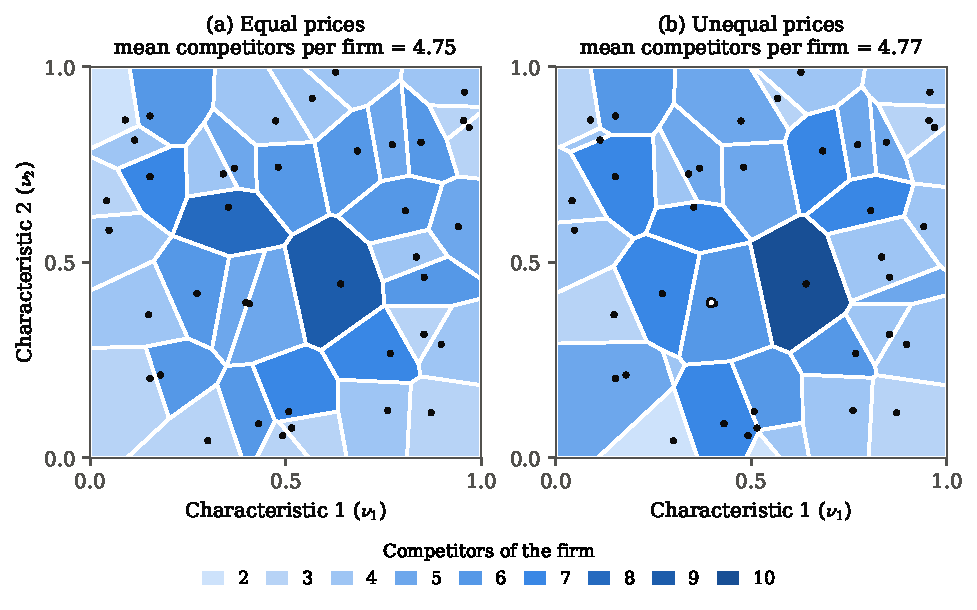
\includegraphics[width=\linewidth]{figures/ch04/voronoi.pdf}
\caption{Market areas of 40 products in a two-dimensional characteristics space. Consumers' ideal points are uniform
on the unit square, mismatch costs are quadratic, and dots mark product locations. Shading gives each firm's number
of competitors. (a) Equal prices: Voronoi cells. The average number of competitors is 4.75 over all 40 firms and
5.83 over the 18 firms whose areas do not touch the boundary. (b) Prices drawn between 1.000 and 1.012: power
diagram. One product (open circle) has no buyers. The average is 4.77 over the 39 active firms and 5.72 over the
18 interior firms. Computed with \texttt{figures/ch04/src/voronoi.py}.}
\label{fig:04-voronoi}
\end{figure}

The averages in the figure lie below six, as the proposition requires. Firms at the edge of the market have few
competitors, which pulls the overall average down. As the number of firms grows, the boundary matters less and
the average approaches six from below. Over random draws of uniform locations with equal prices, the average number
of competitors is 3.72 with 10 firms, 4.87 with 40, 5.43 with 160, 5.72 with 640 and 5.80 with 1,280. For firms
away from the boundary the averages are 5.16, 5.71, 5.87, 5.94 and 5.96.

\begin{remark}[Why competitors are defined by shared boundaries]\label{rem:04-competitor-def}
The definition of \citet{CaplinNalebuff1991} counts $k$ as a competitor of $j$ if a marginal cut in $p_j$
reduces $q_k$. Read as a nonzero derivative, it agrees with the shared-boundary definition when the type density
is positive on the interior of $B$. Read literally, as any loss of demand after a small cut, it counts
second-order losses too. Under the literal reading the bound in \cref{prop:04-cn-six} fails in degenerate
configurations. Place
$J \geq 8$ products at equal prices, equally spaced on a circle, with the quadratic mismatch costs of
\cref{fig:04-voronoi}. Let types be uniform on a disk with the same center. The Voronoi cells are wedges that
all meet at the center, and each shares edges only with its two neighbors. After a cut of size $\eta > 0$ in $p_j$, product $j$ is the strict favorite of every type near the
center, so it takes buyers from every other wedge. For a wedge that touches $j$'s area only at the center, the
lost area is of order $\eta^2$, and its first-order cross-price effect is zero. Under the literal reading every
firm has $J - 1 > 6$ competitors. Under the shared-boundary definition every firm has two, as the proposition
allows.
\end{remark}

\begin{example}[No bound in three dimensions]\label{ex:04-no-bound-3d}
Let $L = 3$ and let a consumer buy the product that minimizes $p_j + \tau\|\nu - x_j\|^2$, as in
\cref{fig:04-voronoi}. At equal prices the market areas are Voronoi cells. Types are uniform on the ball of
radius 2 around the origin, which satisfies A2.
Place $n$ products at $A_i = (a_i, 0, 0)$ and $n$ products at $B_l = (1, b_l, 1)$, with distinct $a_i \in [0, 1]$
and distinct $b_l \in [0, 1]$. The two groups lie on two skew lines. For each pair $(i, l)$ let
\begin{equation*}
z_{il} = \frac{(1 - a_i)^2 + 1 - b_l^2}{2}, \qquad c_{il} = (a_i, b_l, z_{il}).
\end{equation*}
The squared distances from $c_{il}$ to $A_i$ and to $B_l$ both equal $b_l^2 + z_{il}^2$. The squared distance to
any other $A_k$ is larger by $(a_k - a_i)^2 > 0$, and the squared distance to any other $B_k$ is larger by
$(b_k - b_l)^2 > 0$. By continuity, the types near $c_{il}$ on the plane of indifference between $A_i$ and $B_l$
are strictly closer to these two locations than to any other. Since $0 \leq z_{il} \leq 1$, the point $c_{il}$
lies inside the ball. The market areas of the two products therefore share a face of positive area within the
support. All $n^2$ such pairs are competitors under the sharper definition, and every product has positive
demand. With $J = 2n$ firms the average number of competitors is at least $\frac{2n^2}{2n} = n = \frac{J}{2}$,
which grows without bound.
\end{example}

The result matters for empirical work in two ways. A pure characteristics model in one or two dimensions implies a
sparse matrix of cross-price effects, in which a product's diversion goes on average to at most six neighbors. In
three or more dimensions the sparsity depends on the configuration of products (\cref{ex:04-no-bound-3d}). A logit-type model
spreads every product's diversion over all products. These are very different predictions for a merger between
two products, and the choice between them is made when the researcher picks the dimension of the model. The result
also shows that the location models of \cref{sec:04-location}, with one dimension, impose strong restrictions on
preferences, and that richer competition requires more dimensions.

\subsection{Demand systems in product space}\label{sec:04-spaces-product}

The goal of product-space demand analysis is to estimate $q = f(p, z)$ in a form that is flexible and consistent
with consumer theory. Aggregation is the main theoretical issue. Market demand behaves like the demand of a single
utility-maximizing consumer only under restrictions on individual preferences. Two such restrictions are the Gorman
polar form and the price-independent generalized logarithmic (PIGLOG) class (\cref{ch:aids}).
\Cref{tab:04-productspace-systems} summarizes the four classical systems. In the table and in this subsection goods are indexed by $i$ and $k$, as in \cref{ch:aids}. Total expenditure is $y$, and
$w_i = \frac{p_i q_i}{y}$ is the budget share of good $i$.

\begin{table}[htbp]
\centering
\caption{Classical demand systems in product space}
\label{tab:04-productspace-systems}
\footnotesize
\renewcommand{\arraystretch}{1.35}
\begin{tabularx}{\textwidth}{@{}>{\raggedright\arraybackslash}p{2.15cm}>{\raggedright\arraybackslash}p{4.35cm}%
>{\raggedright\arraybackslash}p{1.9cm}>{\raggedright\arraybackslash}p{2.7cm}>{\raggedright\arraybackslash}X@{}}
\toprule
System and source & Demand equation & Price parameters & Restrictions of theory & Main limitation \\
\midrule
Linear expenditure system \citep{Stone1954}
 & $p_iq_i = p_i\gamma_i + \beta_i\big(y - \sum_k p_k\gamma_k\big)$, from Stone-Geary utility $\sum_i\beta_i\ln(q_i -
   \gamma_i)$ with $\sum_i\beta_i = 1$
 & None beyond the $2J - 1$ parameters $(\gamma, \beta)$
 & Adding up, homogeneity and symmetry hold by construction
 & Too few parameters to be flexible. All goods are Hicksian substitutes, and no good is inferior. \\
Rotterdam model \citep{Theil1965,Barten1966}
 & $w_i\,\dd\ln q_i = \theta_i\,\dd\ln\bar Q + \sum_k\pi_{ik}\,\dd\ln p_k$, with $\dd\ln\bar Q = \sum_k w_k\,\dd\ln
   q_k$
 & $\frac{J(J-1)}{2}$ free $\pi_{ik}$
 & Adding up, homogeneity and symmetry are linear restrictions on $(\theta, \pi)$. Negativity needs $[\pi_{ik}]$
   negative semidefinite
 & A local approximation in differentials, with constant coefficients, not derived from a utility function. \\
Indirect translog \citep{ChristensenJorgensonLau1975}
 & $w_i = \frac{\alpha_i + \sum_k\beta_{ik}\ln\frac{p_k}{y}}{\sum_l\alpha_l + \sum_l\sum_k\beta_{lk}\ln\frac{p_k}{y}}$,
   by Roy's identity from a quadratic $\ln V$ in $\ln\frac{p}{y}$
 & $\frac{J(J+1)}{2}$ symmetric $\beta_{ik}$, less a normalization
 & Homogeneity and adding up built in. Symmetry imposed by $\beta_{ik} = \beta_{ki}$
 & Shares nonlinear in parameters. Aggregates only under extra restrictions. \\
Almost Ideal Demand System \citep{DeatonMuellbauer1980a}
 & $w_i = \alpha_i + \sum_k\gamma_{ik}\ln p_k + \beta_i\ln\frac{y}{P}$, with translog price index $\ln P$
 & $\frac{J(J-1)}{2}$ free $\gamma_{ik}$
 & Linear and testable: adding up, homogeneity, symmetry
 & Still of order $J^2$ parameters. Negativity not imposed globally. \\
\bottomrule
\end{tabularx}

\vspace{3pt}
\begin{minipage}{0.97\textwidth}
\footnotesize Notes: Goods are indexed by $i$ and $k$, $y$ is total expenditure and $w_i = \frac{p_iq_i}{y}$ is a
budget share. Parameter symbols are specific to each row. For the AIDS, $\ln P = \alpha_0 + \sum_k\alpha_k\ln p_k
+ \frac{1}{2}\sum_k\sum_l\gamma_{kl}\ln p_k\ln p_l$, and the restrictions are $\sum_i\alpha_i = 1$,
$\sum_i\gamma_{ik} = 0$, $\sum_i\beta_i = 0$ (adding up), $\sum_k\gamma_{ik} = 0$ (homogeneity) and $\gamma_{ik} =
\gamma_{ki}$ (symmetry) \citep[eqs.~8--12]{DeatonMuellbauer1980a}. In the Rotterdam model $\dd\ln\bar Q$ is the
Divisia volume index. Price-parameter counts are after the restrictions of theory.
\end{minipage}
\end{table}

The linear expenditure system was the first system estimated from an explicit utility function
\citep[p.~312]{DeatonMuellbauer1980a}. Consumers buy subsistence quantities $\gamma_i$ first and split the remaining
income in the fixed proportions $\beta_i$. Its cross-price effects are $\frac{\partial q_i}{\partial p_k} =
-\frac{\beta_i\gamma_k}{p_i}$ for $k \neq i$, so the $J^2$ price effects are pinned down by $2J - 1$ parameters. The
Rotterdam model approximates the demand functions themselves in differential form. The translog approximates the
indirect utility function to second order. The Almost Ideal Demand System starts from a class of preferences that
aggregates across consumers and yields shares that are nearly linear in the parameters. \Cref{ch:aids} develops the
AIDS in full, and \cref{rem:05-translog-piglog} states when the translog aggregates.

\casehead{Three problems in practice}
The first problem is dimensionality. A linear system $q = a + Ap$ has $J$ intercepts and $J^2$ price
coefficients. With $J = 50$ brands, as in a cereal aisle, that is 2,500 price coefficients. Symmetry reduces the
count to $\frac{J(J+1)}{2} = 1{,}275$, and the full set of AIDS restrictions to $\frac{J(J-1)}{2} = 1{,}225$. These
numbers exceed what typical market-level data can estimate.

The second problem is instruments. Each demand equation contains all $J$ prices, and every price is endogenous. Write
the equation for good $i$ in market $t$ as $q_{it} = a_i + \sum_k A_{ik}p_{kt} + e_{it}$, and let $z_t$ be a vector
of excluded instruments. The order condition requires at least $J$ instruments. The rank condition requires that
$\E[z_t p_t^\top]$ have rank $J$, so the instruments must move the $J$ prices independently of one another. A single
market-wide cost shifter fails this test. If $z_t$ is a scalar, the first-stage fitted prices $\hat p_{kt} =
\hat\pi_k z_t$ are proportional to one another, and only one linear combination of the row $A_{i\cdot}$ is
identified. Identification needs product-specific shifters, such as ingredient costs that differ across products,
or prices of the same product in other markets (\cref{ch:aids}).

The third problem is consumer heterogeneity. A representative consumer cannot say who gains and who loses from a
price change or a new product. Distributional questions, and substitution patterns that depend on who buys which
product, require explicit heterogeneity. Characteristics models build it in through the taste distribution and
demographics.

\casehead{Four ways forward}
Applied work responds to these problems in four ways. Each buys tractability with an assumption.
\begin{enumerate}
  \item \emph{Aggregate, or study one product.} Group products into a few aggregates, or estimate the residual
  demand of a single firm, as \citet{BakerBresnahan1988} do (\cref{ch:conduct}). This sacrifices the cross-effects
  among products within each aggregate.
  \item \emph{Impose symmetry.} Representative-consumer systems such as CES and logit treat products symmetrically
  up to one or two parameters (\cref{sec:04-repcons}). They suit questions about variety and poorly serve questions
  about which products are close substitutes.
  \item \emph{Impose separability.} Multi-stage budgeting splits goods into groups and estimates a small system within
  each group (\cref{sec:05-separability}). \citet{HausmanLeonardZona1994} and \citet{Hausman1997} follow this route
  with the AIDS at the lowest level.
  \item \emph{Move to characteristics space.} Discrete choice models replace product-indexed parameters with tastes for
  characteristics (\cref{ch:discrete,ch:logit,ch:blp}), at the costs described in \cref{sec:04-spaces-drawbacks}.
\end{enumerate}
The rest of this chapter develops the second route, together with the location models that underlie the fourth.
\Cref{ch:aids} takes the third route, and \cref{ch:discrete,ch:logit,ch:blp} take the fourth.

\section{Representative-consumer demand systems: linear, CES and logit}\label{sec:04-repcons}

\Cref{sec:04-spaces} showed that an unrestricted demand system in product space has far too many parameters.
One remedy imposes symmetry. A \emph{representative consumer} is a single fictitious agent whose demands equal
market demands. If she also treats all products symmetrically, a handful of parameters governs every own and
cross effect. This section develops the three systems of this kind that appear most often in applied work:
linear demand from quadratic utility, constant elasticity of substitution (CES) demand, and the logit. For each
we derive demand, elasticities, diversion and Bertrand markups. We then show that the CES and the logit are also
discrete choice models, which ties this section to the random utility models of \cref{ch:discrete}. A two-sector
version of the CES model, the model of monopolistic competition of \citet{Spence1976} and \citet{DixitStiglitz1977},
asks whether markets supply the right number of products. The section closes with the questions these systems answer
well and a table that compares them.

\subsection{Linear demand from quadratic utility}\label{sec:04-repcons-linear}

The linear demand of \cref{ex:04-linear-duopoly} has a utility foundation. A representative consumer with
income $y$ buys quantities $q_1, \dots, q_J$ of $J$ differentiated products and an amount $z$ of a numeraire good
with price one. Her utility is quasi-linear in the numeraire,
\begin{equation}\label{eq:04-quadratic-utility}
U(q, z) = z + \bar a\sum_{j=1}^J q_j - \frac{1}{2}\Big[\bar b\sum_{j=1}^J q_j^2 + 2\bar g\sum_{j<k}q_jq_k\Big],
\qquad \bar b > \bar g \ge 0
\end{equation}
\citep{SinghVives1984,Vives1999}. The parameter $\bar a$ is the marginal utility of the first unit of any
product. The parameter $\bar b$ measures how fast marginal utility falls with own consumption, and $\bar g$
measures how much consuming one product lowers the marginal utility of another. The products are substitutes
when $\bar g > 0$ and independent when $\bar g = 0$. As $\bar g$ approaches $\bar b$, utility depends only on total
consumption and the products become perfect substitutes.

\begin{proposition}[Linear demand from quadratic utility]\label{prop:04-quadratic}
Let the consumer maximize \eqref{eq:04-quadratic-utility} subject to $z + \sum_j p_jq_j = y$, and suppose the
solution has $q_j > 0$ for every $j$ and $z > 0$. Then:
\begin{enumerate}[label=(\roman*)]
\item Inverse demand is $p_j = \bar a - \bar bq_j - \bar g\sum_{k \ne j}q_k$.
\item With two products, demand is $q_j = a - bp_j + dp_k$ with
\begin{equation*}
a = \frac{\bar a}{\bar b + \bar g}, \qquad b = \frac{\bar b}{\bar b^2 - \bar g^2}, \qquad d = \frac{\bar g}{\bar b^2 - \bar g^2},
\end{equation*}
so that $b > d \ge 0$ and the diversion ratio is $D_{jk} = \frac{d}{b} = \frac{\bar g}{\bar b}$.
\item With $J$ products, for every $k \ne j$,
\begin{equation*}
\frac{\partial q_j}{\partial p_j} = -\frac{\bar b + (J-2)\bar g}{(\bar b - \bar g)[\bar b + (J-1)\bar g]},
\qquad
\frac{\partial q_k}{\partial p_j} = \frac{\bar g}{(\bar b - \bar g)[\bar b + (J-1)\bar g]},
\qquad
D_{jk} = \frac{\bar g}{\bar b + (J-2)\bar g}.
\end{equation*}
A fraction $1 - (J-1)D_{jk} = \frac{\bar b - \bar g}{\bar b + (J-2)\bar g}$ of the sales that product $j$ loses
leaves the group of products.
\end{enumerate}
\end{proposition}

\begin{proof}
For (i), substitute the budget constraint $z = y - \sum_j p_jq_j$ into utility:
\begin{equation*}
y + \sum_{j=1}^J(\bar a - p_j)q_j - \frac{1}{2}\Big[\bar b\sum_{j}q_j^2 + 2\bar g\sum_{j<k}q_jq_k\Big].
\end{equation*}
The derivative with respect to $q_j$ is $\bar a - p_j - \bar bq_j - \bar g\sum_{k\ne j}q_k$. Setting it to zero gives
(i). The Hessian of the objective is $-B$, where $B$ has $\bar b$ on the diagonal and $\bar g$ off it. In matrix form
$B = (\bar b - \bar g)I_J + \bar g\mathbf{1}\mathbf{1}^\top$. Its eigenvalues are $\bar b - \bar g > 0$ (on vectors
orthogonal to $\mathbf{1}$) and $\bar b + (J-1)\bar g > 0$ (on $\mathbf{1}$). The objective is therefore strictly
concave, and the first-order conditions characterize the maximum.

For (ii) and (iii), stack (i) as $p = \bar a\mathbf{1} - Bq$, so that $q = B^{-1}(\bar a\mathbf{1} - p)$ and
$\frac{\partial q}{\partial p^\top} = -B^{-1}$. We claim that
\begin{equation*}
B^{-1} = \frac{1}{\bar b - \bar g}\Big[I_J - \frac{\bar g}{\bar b + (J-1)\bar g}\mathbf{1}\mathbf{1}^\top\Big].
\end{equation*}
To check it, multiply by $B$ and use $\mathbf{1}\mathbf{1}^\top\mathbf{1}\mathbf{1}^\top = J\mathbf{1}\mathbf{1}^\top$:
\begin{align*}
\big[(\bar b - \bar g)I_J + \bar g\mathbf{1}\mathbf{1}^\top\big]\Big[I_J - \frac{\bar g}{\bar b + (J-1)\bar g}\mathbf{1}\mathbf{1}^\top\Big]
&= (\bar b - \bar g)I_J + \Big[\bar g - \frac{\bar g(\bar b - \bar g) + J\bar g^2}{\bar b + (J-1)\bar g}\Big]\mathbf{1}\mathbf{1}^\top \\
&= (\bar b - \bar g)I_J + \Big[\bar g - \frac{\bar g\,[\bar b + (J-1)\bar g]}{\bar b + (J-1)\bar g}\Big]\mathbf{1}\mathbf{1}^\top
= (\bar b - \bar g)I_J .
\end{align*}
The diagonal element of $-B^{-1}$ is
$-\frac{1}{\bar b - \bar g}\big[1 - \frac{\bar g}{\bar b + (J-1)\bar g}\big] = -\frac{\bar b + (J-2)\bar g}{(\bar b - \bar g)[\bar b + (J-1)\bar g]}$,
and the off-diagonal element is $\frac{\bar g}{(\bar b - \bar g)[\bar b + (J-1)\bar g]}$. This proves the derivatives in
(iii). The diversion ratio \eqref{eq:04-diversion-def} is minus their ratio. The fraction that leaves the group is
$1 - \frac{(J-1)\bar g}{\bar b + (J-2)\bar g} = \frac{\bar b - \bar g}{\bar b + (J-2)\bar g}$, which is positive
because $\bar b > \bar g$. Setting $J = 2$ gives $b = \frac{\bar b}{(\bar b - \bar g)(\bar b + \bar g)}$ and
$d = \frac{\bar g}{(\bar b - \bar g)(\bar b + \bar g)}$. The intercept is
$\frac{\bar a(\bar b - \bar g)}{\bar b^2 - \bar g^2} = \frac{\bar a}{\bar b + \bar g}$, which proves (ii).
\end{proof}

Three features of this system matter below. First, cross derivatives are symmetric,
$\frac{\partial q_k}{\partial p_j} = \frac{\partial q_j}{\partial p_k}$, because the Jacobian $-B^{-1}$ is symmetric. This
is the quasi-linear case (i) of \cref{rem:04-symmetry}. Second, the values $\bar a = 10$, $\bar b = \frac{2}{3}$ and
$\bar g = \frac{1}{3}$ give $a = 10$, $b = 2$ and $d = 1$, the numbers of \cref{ex:04-linear-duopoly}. Third, the
linear form holds only on the set of prices at which every product is bought. If $p_2$ is so high that $q_2 = 0$,
product 1 faces $q_1 = \frac{\bar a - p_1}{\bar b}$, with slope $\frac{1}{\bar b}$. This is smaller in absolute value
than $b = \frac{\bar b}{\bar b^2 - \bar g^2}$, so demand is continuous but kinked where the rival drops out.

The system has three parameters only because of symmetry. A general quadratic utility
$z + \bar a^\top q - \frac{1}{2}q^\top Bq$ with any symmetric positive definite $B$ gives the linear system
$q = B^{-1}(\bar a - p)$, with $\frac{J(J+1)}{2}$ slope parameters. That is the linear product-space system of
\cref{sec:04-spaces} with symmetry imposed. The symmetric version replaces it by $\bar b$ and $\bar g$.

\casehead{Crowded markets} The symmetric system has a strong implication for markets with many products.
Suppose $N$ single-product firms (here $N = F = J$) sell the $N$ products at a common marginal cost $c$. At
symmetric prices $p$, part (i) gives each firm the quantity $q = \frac{\bar a - p}{\bar b + (N-1)\bar g}$. By the
inverse semi-elasticity rule of \cref{sec:04-bertrand-single}, a single-product firm sets
$p - c = -q\big(\frac{\partial q_j}{\partial p_j}\big)^{-1}$. Substituting $q$ and the own slope from part (iii),
\begin{equation*}
p - c = \frac{\bar a - p}{\bar b + (N-1)\bar g}\cdot\frac{(\bar b - \bar g)[\bar b + (N-1)\bar g]}{\bar b + (N-2)\bar g}
= \frac{(\bar a - p)(\bar b - \bar g)}{\bar b + (N-2)\bar g}.
\end{equation*}
Write $\bar a - p = (\bar a - c) - (p - c)$ and collect the terms in $p - c$:
\begin{equation}\label{eq:04-linear-symmetric}
(p - c)\big[\bar b + (N-2)\bar g + \bar b - \bar g\big] = (\bar a - c)(\bar b - \bar g)
\quad\Longrightarrow\quad
p - c = \frac{(\bar a - c)(\bar b - \bar g)}{2\bar b + (N-3)\bar g}.
\end{equation}
With $N = 2$ and the numbers above, $p - c = \frac{9 \cdot \frac{1}{3}}{1} = 3$, so $p = 4$ as in
\cref{ex:04-linear-duopoly}. When $\bar g > 0$, the markup falls to zero as $N$ grows. Every new product is a
substitute for every existing one, and a crowded market approaches marginal-cost pricing. The same symmetric
products give consumers bounded gains from variety. At a common price $p$, consumer surplus is utility minus
expenditure, $Nq(\bar a - p) - \frac{1}{2}Nq^2[\bar b + (N-1)\bar g]$. Substituting $q$ gives
\begin{equation*}
CS(N) = Nq(\bar a - p) - \frac{1}{2}Nq(\bar a - p) = \frac{N(\bar a - p)^2}{2[\bar b + (N-1)\bar g]}
\;\longrightarrow\; \frac{(\bar a - p)^2}{2\bar g} \quad \text{as } N \to \infty .
\end{equation*}
The CES and logit systems behave very differently on both counts, as we show next.

\subsection{CES demand}\label{sec:04-repcons-ces}

The CES system is the workhorse of models of monopolistic competition and international trade. A representative
consumer spends income $y$ on $J$ products and has utility
\begin{equation}\label{eq:04-ces-utility}
u(q) = \Big(\sum_{j=1}^J q_j^{\frac{\sigma-1}{\sigma}}\Big)^{\frac{\sigma}{\sigma-1}}, \qquad \sigma > 1 .
\end{equation}
The parameter $\sigma$ is the \emph{elasticity of substitution}. We show below that
$\frac{q_j}{q_k} = (\frac{p_j}{p_k})^{-\sigma}$, so a one percent rise in the relative price $\frac{p_j}{p_k}$
lowers the relative quantity $\frac{q_j}{q_k}$ by $\sigma$ percent. In this section $\sigma$ always denotes the CES
elasticity, as in \cref{ch:aids}. It is a different object from the nesting parameter of the nested logit, which
other chapters also write as $\sigma$. Two other conventions appear in the literature. Some authors write the
inner exponent as $\varsigma = \frac{\sigma - 1}{\sigma} \in (0,1)$, so that $\sigma = \frac{1}{1-\varsigma}$. Others use a different
outer exponent, such as $(\sum_j q_j^\varsigma)^{1-\varsigma}$. Any strictly increasing transformation of $u$ represents the same
preferences, so all of these forms give the same demand.

\begin{proposition}[CES demand and Bertrand pricing]\label{prop:04-ces}
Let the consumer maximize \eqref{eq:04-ces-utility} subject to $\sum_j p_jq_j = y$. Define the \emph{CES price index}
$P^{CES} = \big(\sum_{k=1}^J p_k^{1-\sigma}\big)^{\frac{1}{1-\sigma}}$ and the expenditure shares
$s_j = \frac{p_jq_j}{y}$. Then:
\begin{enumerate}[label=(\roman*)]
\item Demand is
\begin{equation}\label{eq:04-ces-demand}
q_j = \frac{p_j^{-\sigma}}{\sum_{k}p_k^{1-\sigma}}\,y = \Big(\frac{p_j}{P^{CES}}\Big)^{-\sigma}\frac{y}{P^{CES}},
\qquad
s_j = \Big(\frac{p_j}{P^{CES}}\Big)^{1-\sigma},
\end{equation}
and indirect utility is $\frac{y}{P^{CES}}$.
\item The own elasticity is $\varepsilon_j = \sigma - (\sigma - 1)s_j = \sigma(1 - s_j) + s_j$, the cross elasticity
is $\varepsilon_{jk} = (\sigma - 1)s_k$ for $k \ne j$, and the income elasticity is one.
\item The diversion ratio is $D_{jk} = \frac{(\sigma - 1)p_jq_k}{y[\sigma - (\sigma - 1)s_j]}$. Measured in
expenditure, the fraction of the revenue lost by $j$ that goes to $k$ is
$-\frac{\partial(p_kq_k)}{\partial p_j}\big(\frac{\partial(p_jq_j)}{\partial p_j}\big)^{-1} = \frac{s_k}{1 - s_j}$.
\item Suppose each product has constant marginal cost $mc_j$ and firms set prices as in \cref{sec:04-bertrand}. A
single-product firm sets
\begin{equation}\label{eq:04-ces-lerner}
\frac{p_j - mc_j}{p_j} = \frac{1}{\sigma - (\sigma - 1)s_j}.
\end{equation}
A firm that sells the products $\mathcal{J}_f$ gives all of them the same Lerner index,
$\frac{p_j - mc_j}{p_j} = \frac{1}{\sigma - (\sigma - 1)S_f}$, where $S_f = \sum_{k\in\mathcal{J}_f}s_k$.
\end{enumerate}
\end{proposition}

\begin{proof}
(i) Let $\varsigma = \frac{\sigma - 1}{\sigma} \in (0,1)$ and $V(q) = \sum_j q_j^\varsigma$. Since $u = V^{\frac{1}{\varsigma}}$ is a strictly
increasing function of $V$, we may maximize $V$. It is strictly concave, and its marginal utilities are infinite at
zero, so the solution is interior and unique. The first-order condition of the Lagrangian is
$\varsigma q_j^{\varsigma-1} = \lambda p_j$. Since $\varsigma - 1 = -\frac{1}{\sigma}$, it gives
\begin{equation*}
q_j = \Big(\frac{\lambda}{\varsigma}\Big)^{-\sigma}p_j^{-\sigma} \equiv Cp_j^{-\sigma},
\end{equation*}
with $C$ the same for all products. The budget constraint gives $\sum_j p_j\,Cp_j^{-\sigma} = C\sum_j p_j^{1-\sigma} = y$,
so $C = \frac{y}{\sum_k p_k^{1-\sigma}}$. By definition $\sum_k p_k^{1-\sigma} = (P^{CES})^{1-\sigma}$, hence
$q_j = p_j^{-\sigma}(P^{CES})^{\sigma-1}y$, which is \eqref{eq:04-ces-demand}. Multiplying by $\frac{p_j}{y}$ gives
the share. For indirect utility, note that $\sigma\varsigma = \sigma - 1$, so
\begin{equation*}
q_j^\varsigma = \Big(\frac{p_j}{P^{CES}}\Big)^{-\sigma\varsigma}\Big(\frac{y}{P^{CES}}\Big)^\varsigma
= \Big(\frac{p_j}{P^{CES}}\Big)^{1-\sigma}\Big(\frac{y}{P^{CES}}\Big)^\varsigma = s_j\Big(\frac{y}{P^{CES}}\Big)^\varsigma .
\end{equation*}
Summing over $j$ gives $V = (\frac{y}{P^{CES}})^\varsigma$, so $u = \frac{y}{P^{CES}}$. \Cref{prop:05-ces} derives the
expenditure function and the other duality relations.

(ii) Take logs of \eqref{eq:04-ces-demand}: $\ln q_j = -\sigma\ln p_j + (\sigma - 1)\ln P^{CES} + \ln y$. From
$\ln P^{CES} = \frac{1}{1-\sigma}\ln\sum_k p_k^{1-\sigma}$,
\begin{equation*}
\frac{\partial\ln P^{CES}}{\partial\ln p_k} = \frac{1}{1-\sigma}\cdot\frac{(1-\sigma)p_k^{1-\sigma}}{\sum_l p_l^{1-\sigma}} = s_k .
\end{equation*}
Hence $\frac{\partial\ln q_j}{\partial\ln p_j} = -\sigma + (\sigma - 1)s_j$, $\frac{\partial\ln q_j}{\partial\ln p_k} = (\sigma - 1)s_k$
and $\frac{\partial\ln q_j}{\partial\ln y} = 1$. The own elasticity, written as a positive number, is
$\varepsilon_j = \sigma - (\sigma - 1)s_j$.

(iii) By (ii), $\frac{\partial q_k}{\partial p_j} = (\sigma - 1)s_j\frac{q_k}{p_j}$ and
$\frac{\partial q_j}{\partial p_j} = -\varepsilon_j\frac{q_j}{p_j}$. Their ratio is
\begin{equation*}
D_{jk} = \frac{(\sigma - 1)s_jq_k}{\varepsilon_jq_j} = \frac{(\sigma - 1)p_jq_k}{y[\sigma - (\sigma - 1)s_j]},
\end{equation*}
because $\frac{s_j}{q_j} = \frac{p_j}{y}$. For revenues, $\frac{\partial(p_jq_j)}{\partial p_j} = q_j(1 - \varepsilon_j) = -(\sigma - 1)(1 - s_j)q_j$
and $\frac{\partial(p_kq_k)}{\partial p_j} = p_k\frac{\partial q_k}{\partial p_j} = (\sigma - 1)\frac{s_js_ky}{p_j}$. Their ratio, with a minus
sign, is $\frac{s_js_ky}{p_jq_j(1 - s_j)} = \frac{s_k}{1 - s_j}$, since $p_jq_j = s_jy$.

(iv) For a single-product firm, the inverse elasticity rule of \cref{sec:04-bertrand-single} gives
$\frac{p_j - mc_j}{p_j} = \frac{1}{\varepsilon_j}$, and $\varepsilon_j - 1 = (\sigma - 1)(1 - s_j) > 0$. For a
multi-product firm, write the first-order condition \eqref{eq:04-foc-scalar} for $j \in \mathcal{J}_f$ and substitute
the derivatives from (iii):
\begin{equation*}
q_j - (p_j - mc_j)\varepsilon_j\frac{q_j}{p_j} + \sum_{k\in\mathcal{J}_f\setminus\{j\}}(p_k - mc_k)(\sigma - 1)s_j\frac{q_k}{p_j} = 0 .
\end{equation*}
Let $L_k = \frac{p_k - mc_k}{p_k}$, so that $(p_k - mc_k)q_k = L_ks_ky$. Divide by $q_j$ and use $\frac{s_jy}{p_jq_j} = 1$:
\begin{equation*}
1 - L_j\varepsilon_j + (\sigma - 1)\sum_{k\in\mathcal{J}_f\setminus\{j\}}L_ks_k = 0 .
\end{equation*}
Substitute $\varepsilon_j = \sigma - (\sigma - 1)s_j$ and move the term $(\sigma - 1)L_js_j$ into the sum:
\begin{equation*}
\sigma L_j = 1 + (\sigma - 1)\sum_{k\in\mathcal{J}_f}L_ks_k .
\end{equation*}
The right side is the same for every $j \in \mathcal{J}_f$, so the firm's products share one Lerner index $L_f$.
Then $\sigma L_f = 1 + (\sigma - 1)S_fL_f$, and solving gives $L_f = \frac{1}{\sigma - (\sigma - 1)S_f}$.
\end{proof}

Part (ii) shows how little freedom the system has. One parameter governs all substitution. The own elasticity is
a weighted average of $\sigma$ and one, with weight $s_j$ on the unit elasticity of total spending. When $p_k$ rises,
every other product gains demand in the same proportion, $(\sigma - 1)s_k$, however close it is to $k$. With many
small products every own elasticity is close to $\sigma$. Part (iii) restates this in the language of
\cref{sec:04-diversion}. Quantity diversion is proportional to $q_k$, and expenditure diversion is exactly the logit
formula $\frac{s_k}{1 - s_j}$. The quantity ratios do not sum to one, because total spending is fixed while total
units are not.

\casehead{Symmetric firms and the large-group limit} Let $N$ single-product firms ($N = F = J$) share a common
marginal cost. In the symmetric equilibrium $s_j = \frac{1}{N}$, and \eqref{eq:04-ces-lerner} becomes
\begin{equation}\label{eq:04-ces-symmetric}
\frac{p - mc}{p} = \frac{1}{\sigma - \frac{\sigma - 1}{N}} = \frac{N}{\sigma N - \sigma + 1}.
\end{equation}
The Lerner index equals $\frac{2}{\sigma + 1}$ with two firms and falls toward $\frac{1}{\sigma}$ as $N$ grows. In the
limit $p = \frac{\sigma}{\sigma - 1}mc$, the constant markup of monopolistic competition in the model of
\citet{DixitStiglitz1977}. There each firm is too small to affect $P^{CES}$, so it perceives the elasticity $\sigma$.
\Citet{CaplinNalebuff1991} note (footnote 19) that an early version of the Dixit-Stiglitz paper worked with a
continuum of firms, for which this own effect is exactly zero. With finitely many firms it is positive, and
with few firms ignoring it is inappropriate. The exact formula measures the error. With $\sigma = 3$ and $N = 10$
the Lerner index is $\frac{1}{2.8} = 0.357$, against $\frac{1}{3} = 0.333$ in the large-group approximation.

The case $N = 1$ shows why at least two firms are needed. A single seller has $s = 1$ and faces unit-elastic demand
$q = \frac{y}{p}$. Its revenue is fixed at $y$. With $mc > 0$, its profit $y - mc\,\frac{y}{p}$ rises with $p$ toward
the supremum $y$, which no finite price attains, so no finite price is optimal. With $mc = 0$ every price earns $y$,
so the price is indeterminate. With $N \ge 2$ each firm's demand is log-concave in the logarithm of its own price.
By part (ii), the elasticity $\sigma - (\sigma - 1)s_j$ rises with $p_j$ because $s_j$ falls. The log-log
condition of \cref{sec:04-existence-demand} then makes profit quasi-concave in own price. \Citet{CaplinNalebuff1991}
prove that a pure-strategy equilibrium exists with at least two firms and positive costs, and that it is unique in
the duopoly (\cref{sec:04-repcons-cesdc}).

\casehead{Why CES misleads for mergers} Part (iv) says that a CES firm's markup depends only on its combined
expenditure share. A merger of products $j$ and $k$ raises both Lerner indices to
$\frac{1}{\sigma - (\sigma - 1)(s_j + s_k)}$ at given shares. Nothing in this formula refers to how close $j$ and $k$
are. Two near-identical brands and two unrelated products with the same shares produce the same predicted price
increase. A numerical illustration makes the point. Take ten single-product firms with $mc = 1$ and $\sigma = 3$.
In the symmetric equilibrium each has share 0.1, Lerner index 0.357 and price 1.556. Now let firms 1 and 2 merge.
We solve the post-merger first-order conditions of part (iv) by iterating on the Lerner formulas. The merged
firm raises both prices by 3.9 percent, to 1.616, and each of its products' shares falls to 0.094. Each rival raises
its price by 0.06 percent. These predictions hold for every pair of firms, whether the merging products are close or
distant substitutes. The model has no parameter that could tell the two cases apart. For the same reason CES
markups are nearly equal across products whenever shares are small, whatever the pattern of competition.

\begin{remark}[Taste weights and an outside good]\label{rem:04-ces-weights}
\Cref{ch:aids} writes CES utility with weights,
$u(q) = \big(\sum_j a_j^{\frac{1}{\sigma}}q_j^{\frac{\sigma-1}{\sigma}}\big)^{\frac{\sigma}{\sigma-1}}$ with $a_j > 0$
(\cref{prop:05-ces}). The weights act as quality shifters. They change the price index to
$P^{CES} = \big(\sum_k a_kp_k^{1-\sigma}\big)^{\frac{1}{1-\sigma}}$ and the shares to
$s_j = a_j\big(\frac{p_j}{P^{CES}}\big)^{1-\sigma}$. Parts (ii) to (iv) of \cref{prop:04-ces} hold unchanged when
written in terms of these shares. An outside good can be added through a Cobb-Douglas upper tier in $u(q)$ and a
numeraire. The consumer then spends a fixed fraction of income on the differentiated products, and every result
holds with $y$ replaced by that expenditure \citep[Section 8]{CaplinNalebuff1991}.
\end{remark}

\subsection{The logit as the demand of a representative consumer}\label{sec:04-repcons-logit}

The logit is usually derived from a population of consumers with random utility (\cref{ch:discrete}).
\citet{AndersonDePalmaThisse1988} show that the same shares solve the problem of a single consumer with a taste for
variety. Write mean utility as $\delta_j = \tilde\delta_j - \alpha p_j$, where $\tilde\delta_j = x_j\beta + \xi_j$ is
the quality of product $j$ before price is taken into account. The outside good has $\tilde\delta_0 = p_0 = 0$. The
consumer allocates one unit of consumption across the $J + 1$ alternatives, so $q_j$ is the fraction of the unit
that goes to alternative $j$. With a market of size one, $q_j$ is also the market share.

\begin{proposition}[Logit demand from an entropy representative consumer]\label{prop:04-logit-entropy}
Consider the program, with the convention $0\ln 0 = 0$,
\begin{equation}\label{eq:04-entropy}
\max_{q_0, \dots, q_J \ge 0}\; \sum_{j=0}^J(\tilde\delta_j - \alpha p_j)q_j - \sum_{j=0}^J q_j\ln q_j
\qquad\text{subject to}\qquad \sum_{j=0}^J q_j = 1 .
\end{equation}
\begin{enumerate}[label=(\roman*)]
\item The program has a unique solution. It is interior and equals the logit shares
$q_j = \frac{e^{\delta_j}}{\Phi}$, with $\Phi = 1 + \sum_{k=1}^J e^{\delta_k}$.
\item The maximized value is $\ln\Phi$.
\item The same demands solve the quasi-linear program
$\max\; y - \sum_j p_jq_j + \frac{1}{\alpha}\big[\sum_j\tilde\delta_jq_j - \sum_j q_j\ln q_j\big]$ subject to
$\sum_j q_j = 1$. Its maximized value is $y + \frac{1}{\alpha}\ln\Phi$, and the derivative of this value with respect
to $p_j$ equals $-q_j$.
\end{enumerate}
\end{proposition}

\begin{proof}
(i) The objective is continuous on the simplex, which is compact, so a maximum exists. The function
$-q\ln q$ is strictly concave and the other terms are linear, so the objective is strictly concave and the maximum
is unique. The derivative of $-q\ln q$ is $-\ln q - 1$, which tends to $+\infty$ as $q \to 0$. Moving a little
mass from any alternative with positive consumption to one with zero consumption therefore raises the objective.
The maximum is interior, and it solves the first-order conditions of the Lagrangian
$\sum_j\delta_jq_j - \sum_jq_j\ln q_j - \lambda(\sum_j q_j - 1)$:
\begin{equation*}
\delta_j - \ln q_j - 1 - \lambda = 0
\quad\Longrightarrow\quad
q_j = e^{\delta_j}e^{-(1+\lambda)} .
\end{equation*}
The constraint gives $e^{-(1+\lambda)}\sum_{k=0}^J e^{\delta_k} = 1$. Since $\delta_0 = 0$, the sum equals $\Phi$, and
$q_j = \frac{e^{\delta_j}}{\Phi}$.

(ii) At the solution $\ln q_j = \delta_j - \ln\Phi$. The value is
$\sum_j\delta_jq_j - \sum_jq_j(\delta_j - \ln\Phi) = \ln\Phi\sum_jq_j = \ln\Phi$.

(iii) Since $-\sum_j p_jq_j = \frac{1}{\alpha}\sum_j(-\alpha p_j)q_j$, the quasi-linear objective equals $y$ plus
$\frac{1}{\alpha}$ times the objective in \eqref{eq:04-entropy}. It has the same maximizer and the value
$y + \frac{1}{\alpha}\ln\Phi$. Finally, $\frac{\partial}{\partial p_j}\frac{1}{\alpha}\ln\Phi = \frac{1}{\alpha}\cdot\frac{-\alpha e^{\delta_j}}{\Phi} = -q_j$.
\end{proof}

The adding-up constraint does the work of substitution. Without it, the first-order conditions read
$\delta_j - \ln q_j - 1 = 0$ and give $q_j = e^{\delta_j - 1}$. Each demand would then depend only on its own
price, and no product would gain when a rival raised its price. The constraint ties the demands together through
the multiplier $\lambda$, which equals the inclusive value $\ln\Phi$ minus one.

The term $-\sum_jq_j\ln q_j$ is the \emph{entropy} of the consumption profile. It is largest when consumption is
spread evenly, so it represents a taste for variety. In the quasi-linear form of part (iii) the entropy carries
the weight $\frac{1}{\alpha}$, and $\frac{\tilde\delta_j}{\alpha}$ is the dollar value of product $j$'s quality. As
$\alpha$ grows, the taste for variety vanishes relative to money. The consumer then concentrates on the alternative
with the largest net value $\frac{\tilde\delta_j}{\alpha} - p_j$, as buyers of a homogeneous good would. As $\alpha$
falls, variety dominates and consumption spreads out.

The proposition gives the logit two foundations with the same aggregate demand. In the population view, consumer
$i$ has utility $u_{ij} = \delta_j + \epsilon_{ij}$ with i.i.d.\ type-I extreme value shocks and buys one unit of her
best alternative \citep{McFadden1974}. Her expected maximum utility is $\ln\Phi$ plus Euler's constant
(\cref{ch:discrete}). Part (ii) shows that the representative consumer's value has the same form. The log-sum
measure of consumer surplus used in \cref{ch:logit} therefore has a representative-consumer reading as well. Part
(iii) is a version of Roy's identity: the derivative of the value with respect to a price is minus the demand.

\begin{remark}[Perturbed utility and random utility]\label{rem:04-perturbed}
The equivalence extends beyond the logit. Take any additive random utility model with a strictly positive joint
density of shocks and continuously differentiable choice probabilities. Its choice probabilities maximize
$\sum_j\delta_jq_j - \mathcal{C}(q)$ over the interior of the simplex for some function $\mathcal{C}(q)$
\citep[Theorem~2.1, p.~2269]{HofbauerSandholm2002}. This $\mathcal{C}$ is strictly convex on the interior of the simplex, and its gradient grows without
bound near the boundary. For the logit, $\mathcal{C}$ is the negative entropy $\sum_jq_j\ln q_j$. The converse fails. With four
or more alternatives, no additive random utility model generates the demands that maximize
$\sum_j\delta_jq_j + \sum_j\ln q_j$ \citep[Proposition~2.2, p.~2271]{HofbauerSandholm2002}.
\end{remark}

\casehead{IIA, elasticities and diversion} At the solution, $\frac{q_j}{q_k} = e^{\delta_j - \delta_k}$ depends only on
products $j$ and $k$. This is the independence of irrelevant alternatives (IIA). The derivatives
\eqref{eq:04-logit-derivs} give $\varepsilon_j = \alpha p_j(1 - s_j)$, $\varepsilon_{kj} = \alpha p_js_j$ for every $k \ne j$,
and $D_{jk} = \frac{s_k}{1 - s_j}$ (\cref{sec:04-diversion-systems}). The classic illustration is the red bus and the
blue bus. A commuter chooses between a car and a red bus, each with share $\frac{1}{2}$. Now add a blue bus that
is identical to the red one. Intuition says the car keeps $\frac{1}{2}$ and the buses split the other half. The
logit gives each option $\frac{1}{3}$, because it treats the blue bus as a new product with its own taste shock
(\cref{ch:logit}). The entropy view tells the same story. The representative consumer gains $\ln 3 - \ln 2$ utils
from the duplicate, because the entropy term rewards variety itself. This is the ``too many characteristics''
problem of \cref{sec:04-spaces-drawbacks}.

Logit and CES share the same proportional substitution, and both allow quality differences ($\tilde\delta_j$ in
the logit, the weights $a_j$ of \cref{rem:04-ces-weights} in the CES). They differ in what is held fixed and in how
price enters. In the logit, total quantity is fixed and price enters utility in levels. In the CES, total spending
is fixed and price enters through its logarithm, as the next subsection shows. As a result, logit markups are
constant in dollars for a given share, $\frac{1}{\alpha(1 - s_j)}$. CES markups are constant as a fraction of price,
$\frac{1}{\sigma - (\sigma - 1)s_j}$.

\subsection{CES as a discrete choice model*}\label{sec:04-repcons-cesdc}

The CES demand of a representative consumer can also be generated by a population in which each consumer buys only
one product \citep{AndersonDePalmaThisse1987}. Let a mass $M$ of consumers each have income $y$. Consumer $i$ picks
one product and spends all of her income on it, so she buys $\frac{y}{p_j}$ units if she picks $j$. Her utility from
$q$ units of product $j$ is $\ln q + \frac{1}{\sigma - 1}\epsilon_{ij}$, so her indirect utility from choosing $j$ is
\begin{equation}\label{eq:04-ces-rum}
u_{ij} = \ln y - \ln p_j + \frac{1}{\sigma - 1}\epsilon_{ij},
\end{equation}
with $\epsilon_{ij}$ i.i.d.\ type-I extreme value across consumers and products.

\begin{proposition}[CES as a discrete choice model]\label{prop:04-ces-discrete}
Under \eqref{eq:04-ces-rum}, with $\sigma > 1$:
\begin{enumerate}[label=(\roman*)]
\item The probability that a consumer chooses $j$ is $\frac{p_j^{1-\sigma}}{\sum_k p_k^{1-\sigma}}$. This is a logit
in $-\ln p_j$ with coefficient $\sigma - 1$, and it equals the CES expenditure share of \eqref{eq:04-ces-demand}.
\item Expected demand for product $j$ is $\frac{My\,p_j^{-\sigma}}{\sum_k p_k^{1-\sigma}}$, the CES demand of a
representative consumer with income $My$ and elasticity of substitution $\sigma$.
\item Expected maximum utility is $\E[\max_j u_{ij}] = \ln\frac{y}{P^{CES}} + \frac{\gamma_E}{\sigma - 1}$, where
$\gamma_E \approx 0.5772$ is Euler's constant. Up to a constant, it is the logarithm of the representative
consumer's indirect utility.
\end{enumerate}
\end{proposition}

\begin{proof}
(i) Multiplying all utilities by $\sigma - 1 > 0$ does not change choices:
$(\sigma - 1)u_{ij} = (\sigma - 1)\ln y - (\sigma - 1)\ln p_j + \epsilon_{ij}$. The first term is common to all
products and drops out. The logit formula with mean utilities $-(\sigma - 1)\ln p_j$ \citep[eqs.~3.14--3.15]{McFadden1984}
gives
\begin{equation*}
\Pr(j) = \frac{e^{-(\sigma - 1)\ln p_j}}{\sum_k e^{-(\sigma - 1)\ln p_k}} = \frac{p_j^{1-\sigma}}{\sum_k p_k^{1-\sigma}} .
\end{equation*}
(ii) Each of the $M\Pr(j)$ consumers who choose $j$ buys $\frac{y}{p_j}$ units, so expected demand is
$M\frac{y}{p_j}\cdot\frac{p_j^{1-\sigma}}{\sum_kp_k^{1-\sigma}} = \frac{Myp_j^{-\sigma}}{\sum_kp_k^{1-\sigma}}$. This is
\eqref{eq:04-ces-demand} with income $My$.
(iii) For i.i.d.\ type-I extreme value shocks, $\E[\max_j(V_j + \epsilon_{ij})] = \ln\sum_je^{V_j} + \gamma_E$
(\cref{ch:discrete}). With $V_j = (\sigma - 1)(\ln y - \ln p_j)$,
\begin{equation*}
(\sigma - 1)\E\big[\max_j u_{ij}\big] = (\sigma - 1)\ln y + \ln\sum_kp_k^{1-\sigma} + \gamma_E
= (\sigma - 1)\ln y + (1 - \sigma)\ln P^{CES} + \gamma_E .
\end{equation*}
Dividing by $\sigma - 1$ gives the result.
\end{proof}

\Citet{CaplinNalebuff1991} use a version of this equivalence with a numeraire, which they attribute to
\citet{AndersonDePalmaThisse1988b}. Their representative consumer has a CES aggregate of the differentiated goods and a
Cobb-Douglas weight on a numeraire $z$. In the discrete choice
version, a consumer buys $q$ units of a single product $j$ and maximizes $qz^\eta$ subject to $p_jq + z = y$, where
$\eta > 0$ is the Cobb-Douglas exponent of the numeraire. The solution is $q = \frac{y}{(1+\eta)p_j}$ and
$z = \frac{\eta y}{1 + \eta}$. The logarithm of maximized utility is
\begin{equation*}
\ln(qz^\eta) = -\ln p_j + (1 + \eta)\ln\frac{y}{1 + \eta} + \eta\ln\eta .
\end{equation*}
Adding an i.i.d.\ extreme value term gives their eq.~(8.3). They call the distribution Weibull, following earlier
usage for the double exponential. With this representation they prove that the representative-consumer CES model
has a pure-strategy Bertrand-Nash equilibrium for any number $N \ge 2$ of firms with positive costs. The
equilibrium is unique for $N = 2$ (their Proposition 14). Their proof observes that (8.3) is exactly the indirect
utility of their model with Cobb-Douglas preferences and variable demand, for suitably chosen product
characteristics. That model extends \cref{thm:04-cn-existence} beyond unit demand (\cref{sec:04-existence}). The
extreme value density is log-concave, so its existence and duopoly uniqueness results carry over to the CES.
Their footnote 3 adds that \citet{DixitStiglitz1977} and \citet{Spence1976} worked with the limit of infinitely many
firms and did not address existence with finitely many.

The proposition shows that the CES and the logit are two members of one family. Both are logit choice models. In
the logit, price enters utility linearly and each consumer buys one unit. In the CES, price enters through its
logarithm and each consumer spends a fixed budget, with $\sigma - 1$ the coefficient on $-\ln p_j$. This explains the
parallel structure of their elasticities in \cref{tab:04-ces-logit-linear}. It also means that the CES inherits IIA,
a point \citet[p.~230]{Hausman1997} stresses for the valuation of new goods. He credits
\citet{AndersonDePalmaThisse1992} with the analysis of the similarity between the two models
\citep[n.~29]{Hausman1997}.

\subsection{The discrete-choice program of Anderson, de Palma and Thisse*}\label{sec:04-repcons-adt}

\Citet{AndersonDePalmaThisse1992} build a theory of product differentiation on discrete choice. Two sources we
could check describe parts of it. We saw that \citet[n.~29]{Hausman1997} credits the book with the analysis of the
similarity between the CES and the logit. \citet[p.~1282]{AndersonDePalmaNesterov1995} refer to it for the theory of an
approach that starts from a population of consumers with heterogeneous tastes and derives aggregate demand. They
also cite its Chapter 3 for CES demand from a discrete choice model with a constant budget share and
double-exponential tastes (p.~1296). We reconstruct the program, which connects the classical approaches to
differentiation through probabilistic choice, and point to where this book develops each piece. The derivations
are ours.

\casehead{Three approaches to differentiation} The first is \citeauthor{Chamberlin1933}'s
\citeyearpar{Chamberlin1933} monopolistic competition. A representative consumer likes variety, and every product
competes with every other. The CES models of \citet{Spence1976} and \citet{DixitStiglitz1977} are its modern form.
The second is the address approach of \citet{Hotelling1929}, in which products and consumers have locations and
each product competes with its neighbors (\cref{sec:04-location}). The third is the characteristics approach of
\citet{Lancaster1966} and \citet{Gorman1980}, in which products are bundles of characteristics (\cref{sec:04-spaces}).
\Citet[p.~3]{CaplinNalebuff1991} describe the trade-off among them. The symmetric CES models bypass product design
and asymmetries. The multi-dimensional probabilistic choice models of \citet{PerloffSalop1985},
\citet{AndersonDePalma1988} and \citet{AndersonDePalmaThisse1988b,AndersonDePalmaThisse1989} also require symmetric
specifications. The characteristics approach suits product design, but existence of equilibrium had been hard to
establish there.

\casehead{Probabilistic choice} Discrete choice theory describes behavior by choice probabilities $\Pr(j \mid C)$
for each choice set $C$. Luce's axiom gives the simplest coherent family \citep{Luce1959}.

\begin{lemma}[Luce's choice axiom]\label{lem:04-luce}
Let $\mathcal{T}$ be a finite set of alternatives and let $\Pr(j \mid C) > 0$ for every $j \in C \subseteq \mathcal{T}$. Suppose
\begin{equation}\label{eq:04-luce}
\Pr(j \mid \mathcal{T}) = \Pr(j \mid C)\Pr(C \mid \mathcal{T}) \qquad\text{for all } j \in C \subseteq \mathcal{T},
\end{equation}
where $\Pr(C \mid \mathcal{T}) = \sum_{k\in C}\Pr(k \mid \mathcal{T})$. Then there are positive \emph{scale values} $w_j$ with
$\Pr(j \mid C) = \frac{w_j}{\sum_{k\in C}w_k}$ for every $C$. Moreover, \eqref{eq:04-luce} holds if and
only if $\frac{\Pr(j \mid C)}{\Pr(k \mid C)}$ is the same for every $C$ that contains $j$ and $k$.
\end{lemma}

\begin{proof}
Set $w_j = \Pr(j \mid \mathcal{T})$. By \eqref{eq:04-luce},
$\Pr(j \mid C) = \frac{\Pr(j \mid \mathcal{T})}{\Pr(C \mid \mathcal{T})} = \frac{w_j}{\sum_{k\in C}w_k}$. This formula
gives $\frac{\Pr(j \mid C)}{\Pr(k \mid C)} = \frac{w_j}{w_k}$ for every $C$. Conversely, suppose the
ratio does not depend on $C$. Then $\frac{\Pr(k \mid C)}{\Pr(j \mid C)} = \frac{\Pr(k \mid \mathcal{T})}{\Pr(j \mid \mathcal{T})}$ for all
$k \in C$. Summing over $k \in C$ gives $\frac{1}{\Pr(j \mid C)} = \frac{\Pr(C \mid \mathcal{T})}{\Pr(j \mid \mathcal{T})}$, which is
\eqref{eq:04-luce}.
\end{proof}

The ratio condition in the lemma is IIA. With $w_j = e^{v_j}$ and $v_j$ linear in characteristics, the Luce
model is the multinomial logit. \citet[p.~1412]{McFadden1984} notes that psychometrics calls this model the Luce
strict utility model. The same formula follows from random utility $u_{ij} = v_j + \epsilon_{ij}$ with i.i.d.\ type-I
extreme value shocks \citep{McFadden1974}. McFadden adds that the shock may stand for tastes the consumer knows
and the analyst does not, or for randomness in the decision itself. Choice data alone cannot tell the two readings
apart \citep[p.~1412]{McFadden1984}.

\casehead{Relaxing IIA} IIA implies that the cross elasticity of the probability of choosing $k$ with respect to an
attribute of $j$ is the same for every $k \ne j$. \Citet[p.~1414]{McFadden1984} calls this property ``theoretically
implausible in many applications'', while noting that the multinomial logit often fits well in practice. The
generalized extreme value (GEV) family relaxes it. Let $H(w_1, \dots, w_J)$ be nonnegative and homogeneous of degree
one, tend to infinity as any argument does, and have mixed partial derivatives of alternating sign. Then the choice
probabilities are $\frac{\partial\ln H(e^{v_1}, \dots, e^{v_J})}{\partial v_j}$ \citep[eqs.~3.29--3.31,
p.~1421]{McFadden1984}. The logit is the case $H = \sum_jw_j$, and the nested logit is the leading other case
(\cref{ch:logit}). The probit drops the extreme value assumption altogether (\cref{ch:discrete}). In each GEV model,
$\ln H$ is expected maximum utility up to a constant, so the log-sum welfare measure generalizes.

\casehead{Representative consumers} \Cref{sec:04-repcons-logit,sec:04-repcons-cesdc} give the
representative consumers of the logit and the CES. \Citet[p.~1406]{McFadden1984} cautions that this is
special. The expectation of a consumer's indirect utility over unobservables need not have the properties of an
indirect utility function. Known sufficient conditions for a choice model to come from a population of utility
maximizers are restrictive. The logit and the CES are cases in which both foundations hold exactly, which is part
of their appeal for theory.

\casehead{The characteristics approach} \Citet{AndersonDePalmaThisse1989} relate discrete choice demand to the
characteristics approach. \Citet[p.~23]{CaplinNalebuff1991} credit this paper and \citet{AndersonDePalmaThisse1988b}
with illuminating a connection. It links representative-agent models, such as the CES of Dixit, Stiglitz and
Spence, to models with heterogeneous consumers. A geometric fact suggests what an address model must do to mimic
the logit. With equal shares, the logit makes every product an equally close substitute for every other. In an
address model this calls for every pair of products to be equally far apart. Points that are pairwise equidistant
form a regular simplex, and $J$ such points need a space of at least $J - 1$ dimensions. An address model with logit
substitution among $J$ products therefore needs many characteristics, which is the ``too many characteristics''
problem of \cref{sec:04-spaces-drawbacks} in geometric form.

\casehead{Oligopoly and variety} With symmetric logit or CES demand, price competition, free entry and the optimal
number of products have closed forms. The same questions can be posed for any distribution of i.i.d.\ tastes, as
in the oligopoly model of \citet{AndersonDePalmaNesterov1995}. \Cref{sec:04-repcons-monocomp} treats the
representative-consumer benchmark of monopolistic competition. \Cref{sec:04-logit-entry} derives the symmetric logit
oligopoly, extends it to general i.i.d.\ tastes and compares the results with the location models of
\cref{sec:04-location}.

\subsection{Monopolistic competition and optimal variety}\label{sec:04-repcons-monocomp}

\citet{Chamberlin1933} introduced \emph{monopolistic competition} to describe an industry of single-product firms with
three properties \citep[Section 7.2]{Tirole1988}. Each firm faces a downward-sloping demand curve. Each firm earns
zero profit. A price change by one firm has a negligible effect on the demand of every other firm. The free-entry
equilibrium on Salop's circle (\cref{sec:04-salop}) has the first two properties. The third separates monopolistic
competition from oligopoly with free entry, because it says that no product has a close neighbor. Tirole notes that
this absence of cross effects has been widely criticized. The model's purpose is to set strategic interaction aside
and isolate one question: how many products does a market supply?

\casehead{The excess capacity argument} An old view held that monopolistic competition produces too many firms, each
too small to exhaust economies of scale. At a zero-profit equilibrium the residual demand curve is tangent to the
average cost curve. The tangency lies where average cost still falls, so output is below the scale that minimizes
average cost. \Citet[Section 7.2]{Tirole1988} shows that this reasoning is flawed. If no other firm sells the same
good, the good may be worth introducing even when its output does not exhaust scale economies. With average cost
$c + \frac{\phi}{q}$, as in the location models, the efficient scale is infinite and every product falls short of it.
The argument therefore needs a second firm that sells the same good. The first firm's demand curve is then horizontal
at the rival's price. Both firms can break even only at the efficient scale, so no excess capacity arises.

\casehead{Two externalities} The comparison of free entry with the optimum turns on two effects of opposite sign
\citep[Section 7.2]{Tirole1988}. The first is the \emph{nonappropriability} of surplus. An entrant cannot capture the
whole consumer surplus its product creates, which pushes toward too few products. The second is \emph{business
stealing}. An entrant takes customers from rivals whose prices exceed marginal cost, and it ignores the margins they
lose. This pushes toward too many products. In general either effect can dominate, and only specific models give a
definite answer.

\casehead{The two-sector model} \Citet{Spence1976} and \citet{DixitStiglitz1977} gave the question a tractable form.
\Citet[Section 7.5.2]{Tirole1988} presents the model with a CES sub-utility. Following his footnote 40, we use the
more general additive form of \citet{DixitStiglitz1977}, and the derivations below are ours. A representative consumer with income
$y$ buys a numeraire $z$ and quantities $q_j$ of $N$ differentiated products. Her utility and budget constraint are
\begin{equation}\label{eq:04-dss-utility}
U\Big(z, \sum_{j=1}^N\chi(q_j)\Big), \qquad z + \sum_{j=1}^Np_jq_j = y ,
\end{equation}
where $U$ is increasing and quasi-concave, and the \emph{sub-utility} $\chi$ is increasing and strictly concave with
$\chi(0) = 0$. All products enter symmetrically, so entry adds variety but no product has a neighbor. Each producer
pays a fixed cost $\phi$ and a constant marginal cost $c$, both in units of the numeraire. Free entry drives profits to
zero, so profits do not enter the consumer's income. Two functions of $q$ summarize $\chi$. The first is the
elasticity of the demand for one product, $\varepsilon(q) = -\frac{\chi'(q)}{q\chi''(q)}$, which we assume exceeds one.
The second is the \emph{rate of appropriability},
\begin{equation}\label{eq:04-appropriability}
\mathcal{R}(q) = \frac{q\chi'(q)}{\chi(q)} ,
\end{equation}
the ratio of a firm's revenue to the gross surplus its product creates \citep[Section 7.5.2]{Tirole1988}. Strict
concavity and $\chi(0) = 0$ give $\chi(q) > q\chi'(q)$, so $\mathcal{R}(q) < 1$. \Citet[p.~54]{MankiwWhinston1986}
isolate the same comparison in their model of product diversity. Measured in units of sub-utility, the marginal
entrant adds $\chi(q)$ to gross surplus and earns $\chi'(q)q$, and the gap is the diversity effect.

\begin{proposition}[Free entry and the optimum with a representative consumer]\label{prop:04-dss}
Let utility be \eqref{eq:04-dss-utility}, and let $N$ be large enough that each firm takes as given the ratio of
marginal utilities $\lambda = \frac{U_V}{U_z}$, where $V = \sum_j\chi(q_j)$ and subscripts denote partial derivatives.
Assume that each firm's profit is strictly concave in its output.
\begin{enumerate}[label=(\roman*)]
\item In the symmetric free-entry equilibrium each firm charges $p = \frac{\varepsilon(q)}{\varepsilon(q) - 1}\,c$ and
sells the quantity $q^*$ that solves
\begin{equation}\label{eq:04-dss-market}
\frac{cq}{\varepsilon(q) - 1} = \phi .
\end{equation}
\item A planner who prices at marginal cost and covers fixed costs with a lump-sum tax chooses the output per product
$q^o$ and the number of products $N^o$. The first-best output per product solves
\begin{equation}\label{eq:04-dss-optimum}
cq\,\frac{1 - \mathcal{R}(q)}{\mathcal{R}(q)} = \phi .
\end{equation}
\item Firms are too large, $q^* > q^o$, if $\mathcal{R}'(q^*) > 0$. They are too small if $\mathcal{R}'(q^*) < 0$, and
of optimal size if $\mathcal{R}'(q^*) = 0$.
\item Let $\chi(q) = q^\varsigma$ with $\varsigma = \frac{\sigma - 1}{\sigma}$ and $\sigma > 1$, and let
$U = z^{1-\gamma}\big(\sum_jq_j^\varsigma\big)^{\frac{\gamma}{\varsigma}}$ with $\gamma \in (0,1)$. Then
\begin{equation}\label{eq:04-dss-ces}
p = \frac{\sigma c}{\sigma - 1}, \qquad q^* = q^o = \frac{(\sigma - 1)\phi}{c}, \qquad
N^* = \frac{\gamma y}{\sigma\phi}, \qquad N^o = \frac{\gamma y}{(\sigma - 1 + \gamma)\phi} ,
\end{equation}
so the market supplies too few products, $\frac{N^o}{N^*} = \frac{\sigma}{\sigma - 1 + \gamma} > 1$.
\end{enumerate}
\end{proposition}

\begin{proof}
(i) Substitute the budget constraint for $z$. The first-order condition for $q_j$ is $U_V\chi'(q_j) = U_zp_j$, so the
inverse demand for product $j$ is $p_j = \lambda\chi'(q_j)$. A firm that takes $\lambda$ as given maximizes
$[\lambda\chi'(q) - c]q - \phi$. Its first-order condition is $\lambda[\chi'(q) + q\chi''(q)] = c$. By the definition
of $\varepsilon$, $q\chi''(q) = -\frac{\chi'(q)}{\varepsilon(q)}$, so the condition reads
$p\big(1 - \frac{1}{\varepsilon}\big) = c$. This gives the price and $p - c = \frac{c}{\varepsilon - 1}$. Zero profit,
$(p - c)q = \phi$, then gives \eqref{eq:04-dss-market}.

(ii) With $N$ products of output $q$ each, the consumer gets $z = y - N(\phi + cq)$ and $V = N\chi(q)$. The planner
maximizes $U\big(y - N(\phi + cq), N\chi(q)\big)$. The first-order conditions for $q$ and $N$ are
\begin{equation*}
-U_zNc + U_VN\chi'(q) = 0, \qquad -U_z(\phi + cq) + U_V\chi(q) = 0 .
\end{equation*}
Let $\lambda^o = \frac{U_V}{U_z}$ at the optimum. The first condition gives $\lambda^o\chi'(q) = c$, so the consumer's
marginal valuation equals marginal cost. The second gives $\lambda^o\chi(q) = \phi + cq$. Dividing the second by the
first,
\begin{equation*}
\frac{\chi(q)}{\chi'(q)} = \frac{\phi + cq}{c}
\quad\Longrightarrow\quad
\frac{cq}{\mathcal{R}(q)} = \phi + cq
\quad\Longrightarrow\quad
cq\Big(\frac{1}{\mathcal{R}(q)} - 1\Big) = \phi ,
\end{equation*}
which is \eqref{eq:04-dss-optimum}.

(iii) Let $g(q) = cq\frac{1 - \mathcal{R}(q)}{\mathcal{R}(q)} = c\big[\frac{\chi(q)}{\chi'(q)} - q\big]$. Its derivative is
$c\frac{\chi'^2 - \chi\chi''}{\chi'^2} - c = -\frac{c\chi\chi''}{\chi'^2} > 0$, so $g$ is strictly increasing and $q^o$ is
the unique solution of $g(q) = \phi$, which is \eqref{eq:04-dss-optimum}. Next, differentiate $\ln\mathcal{R} = \ln q + \ln\chi' - \ln\chi$:
\begin{equation*}
\frac{\mathcal{R}'(q)}{\mathcal{R}(q)} = \frac{1}{q} + \frac{\chi''}{\chi'} - \frac{\chi'}{\chi}
= \frac{1}{q}\Big[1 - \frac{1}{\varepsilon(q)} - \mathcal{R}(q)\Big] .
\end{equation*}
So $\mathcal{R}' > 0$ exactly when $\mathcal{R} < \frac{\varepsilon - 1}{\varepsilon}$. Taking reciprocals and
subtracting one, this holds exactly when $\frac{1 - \mathcal{R}}{\mathcal{R}} > \frac{1}{\varepsilon - 1}$. At $q^*$,
\eqref{eq:04-dss-market} then gives
\begin{equation*}
g(q^*) - \phi = cq^*\Big[\frac{1 - \mathcal{R}(q^*)}{\mathcal{R}(q^*)} - \frac{1}{\varepsilon(q^*) - 1}\Big],
\end{equation*}
which has the sign of $\mathcal{R}'(q^*)$. If it is positive, $g(q^*) > \phi = g(q^o)$, and $q^* > q^o$ because $g$
is increasing. The other two cases follow in the same way.

(iv) For $\chi(q) = q^\varsigma$, $\chi' = \varsigma q^{\varsigma - 1}$ and $q\chi'' = \varsigma(\varsigma - 1)q^{\varsigma - 1}$,
so $\varepsilon = \frac{1}{1 - \varsigma} = \sigma$ and $\mathcal{R} = \varsigma$ is constant. Part (i) gives
$p = \frac{\sigma c}{\sigma - 1}$ and $\frac{cq^*}{\sigma - 1} = \phi$. Part (iii) with $\mathcal{R}' = 0$ gives
$q^o = q^*$. The upper tier is Cobb-Douglas in $z$ and the CES index $(\sum_jq_j^\varsigma)^{\frac{1}{\varsigma}}$, which
is homogeneous of degree one. The consumer therefore spends the share $\gamma$ of income on the differentiated
products, $N^*pq^* = \gamma y$. Since $pq^* = \frac{\sigma c}{\sigma - 1}\cdot\frac{(\sigma - 1)\phi}{c} = \sigma\phi$, we get
$N^* = \frac{\gamma y}{\sigma\phi}$. For the planner, symmetric outputs give the CES index $qN^{\frac{1}{\varsigma}}$, so
\begin{equation*}
\ln U = (1 - \gamma)\ln\big[y - N(\phi + cq)\big] + \gamma\ln q + \frac{\gamma}{\varsigma}\ln N .
\end{equation*}
At $q = q^o$ we have $\phi + cq^o = \sigma\phi$. The first-order condition for $N$ is
$\frac{(1 - \gamma)\sigma\phi}{y - N\sigma\phi} = \frac{\gamma}{\varsigma N}$, so $N\sigma\phi[(1 - \gamma)\varsigma + \gamma] = \gamma y$.
Since $(1 - \gamma)\varsigma + \gamma = \frac{\sigma - 1 + \gamma}{\sigma}$, this gives $N^o$.
\end{proof}

The proposition separates the two margins. Output per product depends only on $\chi$, $c$ and $\phi$, and the rate of
appropriability decides how it compares with the optimum. When $\mathcal{R}$ rises with $q$, a firm captures a growing
share of the surplus it creates as it expands. It then has a stronger incentive to expand than the planner, as
\citet[Section 7.5.2]{Tirole1988} explains. When $\mathcal{R}$ falls, firms are too small, which is the case of excess
capacity. With CES sub-utility the two forces balance and firm size is optimal. The number of products then carries
the whole distortion. In part (iv) the market charges $\frac{\sigma c}{\sigma - 1}$ against the planner's $c$. The
planner therefore draws spending from the numeraire into the differentiated sector and finances more products of the
same size. The gap closes as $\gamma \to 1$, when there is no numeraire to draw from.

The benchmark matters. The first best of part (ii) needs lump-sum taxes to cover the losses of marginal-cost pricing.
\Citet[p.~1293]{AndersonDePalmaNesterov1995} argue that the relevant benchmark for a market is the optimum subject to
zero profits. They also note that a CES example yields too few products relative to the first best, as in part (iv).
For the utility $z^{1-\gamma}[\sum_j\chi(q_j)]^\gamma$ they report the comparison of \citet{DixitStiglitz1977} with this
constrained optimum (p.~1296). Relative to it, the market supplies too many products when $\mathcal{R}$ falls with $q$
and too few when it rises. With constant $\mathcal{R}$, the CES case, the equilibrium and constrained-optimal numbers
of products coincide (p.~1297). The shortfall in part (iv) is relative to the first best. Dixit and
Stiglitz regard a rising $\mathcal{R}$ as the plausible case, so that markets underprovide variety. Anderson, de Palma
and Nesterov object that a rising $\mathcal{R}$ makes total demand for the differentiated goods fall, at given prices,
as products are added. They find a falling $\mathcal{R}$ more plausible, which gives too many products.

\Citet[Section 7.5.2]{Tirole1988} adds that later work, such as \citet{PerloffSalop1985}, gave monopolistic
competition firmer foundations. These models replace the representative consumer by a population whose valuations of the
brands are drawn independently from a distribution, and each consumer buys one brand. \Cref{sec:04-logit-entry} takes
this route. Its model of i.i.d.\ tastes contains the logit as a special case and gives a sharp answer on variety.

\subsection{What symmetric systems are good for}\label{sec:04-repcons-uses}

Symmetric representative-consumer systems answer some questions well and others badly. They are good for questions
about the number of products. Do markets provide too many or too few varieties? How much do consumers gain from new
varieties? How should a price index adjust when varieties enter or exit? They are poor guides to questions that hinge
on which products are close substitutes, such as mergers.

The gains from variety have closed forms. Suppose a CES product enters and takes expenditure share $s$. Before entry
$(P^{CES}_{\mathrm{before}})^{1-\sigma} = \sum_{k\,\mathrm{old}}p_k^{1-\sigma} = (1 - s)(P^{CES}_{\mathrm{after}})^{1-\sigma}$,
because the new product's share of $(P^{CES}_{\mathrm{after}})^{1-\sigma}$ is $s$. Taking logs,
\begin{equation}\label{eq:04-ces-variety}
\ln\frac{P^{CES}_{\mathrm{before}}}{P^{CES}_{\mathrm{after}}} = -\frac{1}{\sigma - 1}\ln(1 - s) .
\end{equation}
The left side is the log change in real income $\frac{y}{P^{CES}}$, holding nominal income and the prices of
continuing products fixed. The exact proportional gain in real income is $(1 - s)^{-\frac{1}{\sigma - 1}} - 1$,
which is close to the log change when that change is small. With $N$ symmetric products at a common price $p$,
$P^{CES} = pN^{\frac{1}{1-\sigma}}$ and real income is $\frac{y}{p}N^{\frac{1}{\sigma-1}}$, unbounded in $N$. In the
logit, part (iii) of \cref{prop:04-logit-entropy} gives the gain from an entrant with share $s$ in a market of size
$M$: $\Delta CS = \frac{M}{\alpha}\ln\frac{\Phi_{\mathrm{after}}}{\Phi_{\mathrm{before}}} = -\frac{M}{\alpha}\ln(1 - s)$. With
$N$ symmetric products, consumer surplus grows like $\frac{M}{\alpha}\ln N$. The quadratic model of
\cref{sec:04-repcons-linear} bounds the gains instead. These formulas explain why trade theory relies on the CES.
\citet{Krugman1980} combines CES preferences with scale economies to explain trade between similar countries.
\citet{Melitz2003} adds productivity differences across firms inside the same CES framework.
The CES has also been applied to the introduction of new products \citep[p.~230, n.~30]{Hausman1997}, for example by
\citet{Feenstra1994}, who adjusts import price indices for new and disappearing varieties. His exact index multiplies
the price index of continuing varieties with unchanged taste parameters by the ratio of their current to previous
expenditure share, raised to the power $\frac{1}{\sigma - 1}$ \citep[Proposition~1, p.~159]{Feenstra1994}. With no exits and unchanged prices of
continuing varieties, this is \eqref{eq:04-ces-variety}. \Cref{prop:10-feenstra} states and proves the result.

The same formulas show the danger. Each new product's value depends only on its share and one substitution
parameter, never on how similar it is to existing products. \Citet[p.~230]{Hausman1997} writes that the IIA problem
of the logit ``typically leads to a vast overestimate of the consumer's surplus from a new good''. He argues that
the CES shares the problem. He estimates a CES demand for cereal brands by nonlinear two-stage least squares and
reports an elasticity of substitution of 2.13 \citep[p.~231]{Hausman1997}.
The implied consumer surplus from the introduction of Apple-Cinnamon Cheerios is about three times his estimate of
\$78.1 million per year from a flexible multilevel demand system (\cref{ch:newgoods}). \Cref{tab:04-ces-logit-linear}
collects the properties of the three systems.

\begin{table}[htbp]
\centering
\caption{Linear, CES and logit demand compared}\label{tab:04-ces-logit-linear}
\footnotesize
\renewcommand{\arraystretch}{1.55}
\begin{tabularx}{\textwidth}{@{}>{\raggedright\arraybackslash}p{2.35cm}>{\raggedright\arraybackslash}X>{\raggedright\arraybackslash}X>{\raggedright\arraybackslash}X@{}}
\toprule
 & Linear (quadratic utility) & CES & Logit \\
\midrule
Representative utility
 & $z + \bar a\sum_jq_j - \frac{\bar b}{2}\sum_jq_j^2 - \bar g\sum_{j<k}q_jq_k$
 & $\big(\sum_jq_j^{\frac{\sigma-1}{\sigma}}\big)^{\frac{\sigma}{\sigma-1}}$ with $\sum_jp_jq_j = y$
 & $\sum_{j=0}^J\delta_jq_j - \sum_{j=0}^Jq_j\ln q_j$ with $\sum_{j=0}^Jq_j = 1$ \\
Parameters
 & $\bar a$, $\bar b$, $\bar g$
 & $\sigma$, plus $J - 1$ taste weights if qualities differ
 & $\alpha$ and the qualities $\tilde\delta_1, \dots, \tilde\delta_J$ \\
Demand
 & $q_j = a - bp_j + dp_k$ when $J = 2$
 & $q_j = \big(\frac{p_j}{P^{CES}}\big)^{-\sigma}\frac{y}{P^{CES}}$
 & $s_j = \frac{e^{\delta_j}}{\Phi}$ \\
Own elasticity $\varepsilon_j$
 & $\frac{bp_j}{q_j}$
 & $\sigma - (\sigma - 1)s_j$
 & $\alpha p_j(1 - s_j)$ \\
Cross elasticity $\varepsilon_{jk}$
 & $\frac{dp_k}{q_j}$
 & $(\sigma - 1)s_k$
 & $\alpha p_ks_k$ \\
Diversion $D_{jk}$
 & $\frac{\bar g}{\bar b + (J-2)\bar g}$, equal to $\frac{d}{b}$ when $J = 2$
 & $\frac{(\sigma-1)p_jq_k}{y[\sigma - (\sigma-1)s_j]}$ in units, $\frac{s_k}{1 - s_j}$ in expenditure
 & $\frac{s_k}{1 - s_j}$ \\
Single-product markup
 & $p_j - c = \frac{q_j}{b}$
 & $\frac{p_j - mc_j}{p_j} = \frac{1}{\sigma - (\sigma - 1)s_j}$
 & $p_j - mc_j = \frac{1}{\alpha(1 - s_j)}$ \\
Multi-product firm
 & joint owner of two products: $p - c = \frac{a - (b - d)c}{2(b - d)}$
 & common Lerner index $\frac{1}{\sigma - (\sigma - 1)S_f}$
 & common markup $\frac{1}{\alpha(1 - S_f)}$ \\
$N$ symmetric firms
 & $p - c = \frac{(\bar a - c)(\bar b - \bar g)}{2\bar b + (N-3)\bar g} \to 0$
 & $\frac{p - c}{p} = \frac{N}{\sigma N - \sigma + 1} \to \frac{1}{\sigma}$
 & $p - c = \frac{N}{\alpha(N - 1)} \to \frac{1}{\alpha}$ \\
Own-cost pass-through, rivals' prices fixed
 & $\frac{1}{2}$
 & $\frac{\sigma}{\sigma - 1}$ in the limit $s_j \to 0$
 & $1 - s_j$ \\
Existence and uniqueness
 & unique where all products sell (best responses are contractions)
 & exists for $N \ge 2$ and $mc_j > 0$, unique for $N = 2$
 & exists and is unique for any ownership (\cref{thm:04-logit-unique}) \\
Gain from variety
 & bounded: $CS \to \frac{(\bar a - p)^2}{2\bar g}$ as $N \to \infty$
 & real income rises by the factor $(1 - s)^{-\frac{1}{\sigma-1}}$, unbounded in $N$
 & $\Delta CS = -\frac{M}{\alpha}\ln(1 - s)$, growing like $\frac{M}{\alpha}\ln N$ \\
\bottomrule
\end{tabularx}
\par\smallskip
\begin{minipage}{\textwidth}
\footnotesize Notes: $s_j$ is the expenditure share (CES) or market share (logit) of product $j$. $S_f$ is the
combined share of firm $f$, and $s$ is the share of an added product after entry. Linear entries for $N$ firms use the
symmetric $J$-product system of \cref{prop:04-quadratic} with $J = N$. The logit markup for $N$ symmetric firms
assumes no outside good, and with an outside good it is $\frac{1}{\alpha(1 - s)}$. Linear best responses have slopes
summing to $\frac{(J-1)\bar g}{2[\bar b + (J-2)\bar g]} < \frac{1}{2}$. CES existence and uniqueness are due to
\citet{CaplinNalebuff1991}. Sources: \cref{prop:04-quadratic,prop:04-ces,prop:04-logit-entropy,prop:04-logit-markup},
\eqref{eq:04-linear-symmetric}, \eqref{eq:04-ces-symmetric}, \eqref{eq:04-ces-variety} and
\cref{sec:04-logit-entry}.
\end{minipage}
\end{table}

\section{Location models: prices, products and entry in characteristics space}\label{sec:04-location}

Location models describe differentiation by a position in a space of characteristics. Each consumer has an ideal
point, and buying a product away from it costs her a \emph{transport cost}, also called a mismatch cost. The models
predate empirical demand analysis by decades. They remain the cleanest setting for three questions that the
symmetric systems of \cref{sec:04-repcons} cannot pose. Does a price equilibrium exist when demand has kinks or
jumps? How do firms choose products when they anticipate price competition? Does free entry produce too many or too
few products? \Cref{sec:06-hotelling} introduces the Hotelling and Salop models as demand models. Here we develop
their equilibrium theory, add the vertical model of quality choice and a symmetric oligopoly with logit or other
i.i.d.\ tastes, and compare entry outcomes across models. Throughout, $\tau > 0$ is the transport cost parameter, $\phi$ is a fixed cost of entry, and
the location of product $j$ is a one-dimensional characteristic $x_j$.

\subsection{Hotelling's line with linear transport costs}\label{sec:04-hotelling-linear}

\begin{assumption}[Hotelling duopoly]\label{ass:04-hotelling}
(i) A mass $M$ of consumers is uniformly distributed on $[0,1]$. A consumer at $x$ buys one unit from the firm that
minimizes her delivered price $p_j + T(|x - x_j|)$, where $T$ is the transport cost function. (ii) Her reservation
value $\bar u$ is high enough that every consumer buys, so the market is \emph{covered}. (iii) Two firms located at
$x_1 = a$ and $x_2 = 1 - b$, with $a + b < 1$, produce at constant marginal cost $c$ and set prices simultaneously.
(iv) Transport costs are linear, $T(d) = \tau d$, or quadratic, $T(d) = \tau d^2$.
\end{assumption}

The parameters $a$ and $b$ measure how far each firm sits from its own end of the line. In this section they denote
locations and are unrelated to the demand parameters of \cref{ex:04-linear-duopoly}. Unless stated otherwise we take $a, b \ge 0$. Write $\Delta x = x_2 - x_1 = 1 - a - b$ for the distance between the firms. Firm 1 has a
\emph{hinterland} $[0, a]$ of consumers to its left, and firm 2 has the hinterland $[1 - b, 1]$.

\casehead{Demand with linear costs} A consumer between the firms, $x \in [a, 1-b]$, prefers firm 1 when
$p_1 + \tau(x - a) < p_2 + \tau(1 - b - x)$. The indifferent consumer solves this with equality:
\begin{equation*}
2\tau x = p_2 - p_1 + \tau(1 + a - b)
\quad\Longrightarrow\quad
\tilde x = \frac{1 + a - b}{2} + \frac{p_2 - p_1}{2\tau} .
\end{equation*}
Consumers in a hinterland compare two delivered prices that rise at the same rate $\tau$ as they move away. A consumer
at $x \ge 1 - b$ prefers firm 1 if and only if $p_1 + \tau(x - a) < p_2 + \tau(x - 1 + b)$, that is, if
$p_1 < p_2 - \tau\Delta x$. The comparison does not depend on $x$, so the whole hinterland switches at once. Firm 1's
demand is therefore
\begin{equation}\label{eq:04-hotelling-linear-demand}
q_1(p_1, p_2) =
\begin{cases}
M & \text{if } p_1 < p_2 - \tau\Delta x,\\[2pt]
M\Big[\frac{1 + a - b}{2} + \frac{p_2 - p_1}{2\tau}\Big] & \text{if } |p_1 - p_2| \le \tau\Delta x,\\[2pt]
0 & \text{if } p_1 > p_2 + \tau\Delta x .
\end{cases}
\end{equation}
At $p_1 = p_2 - \tau\Delta x$ the middle expression equals $M(1 - b)$, so demand jumps by $Mb$, the mass of firm 2's
hinterland. At $p_1 = p_2 + \tau\Delta x$ it equals $Ma$ and demand jumps to zero. Demand is continuous only when
both firms sit at the ends, $a = b = 0$. Panel (a) of \cref{fig:04-hotelling} shows the mechanism. When firm 1
cuts its price to $p_2 - \tau\Delta x$, its delivered-price schedule lies weakly below firm 2's everywhere, and the
consumers beyond $x_2$ switch together.

\begin{figure}[htbp]
\centering
\begin{subfigure}[b]{0.48\textwidth}
\centering
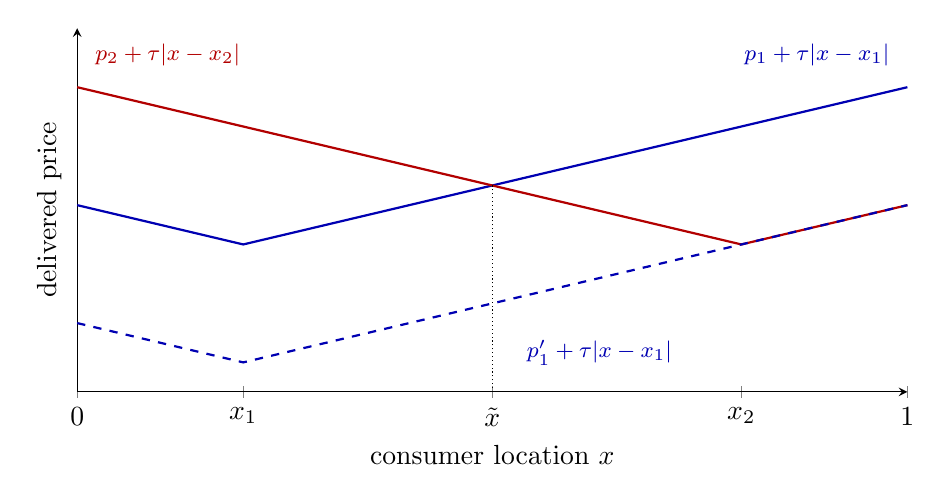
\begin{tikzpicture}
\begin{axis}[
  width=\linewidth, height=6.2cm,
  xmin=0, xmax=1, ymin=0.25, ymax=2.1,
  axis lines=left,
  xtick={0,0.2,0.5,0.8,1},
  xticklabels={$0$,$x_1$,$\tilde x$,$x_2$,$1$},
  ytick=\empty,
  xlabel={consumer location $x$},
  ylabel={delivered price},
  samples=201, domain=0:1,
  clip=false]
\addplot[thick, blue!70!black] {1 + abs(x - 0.2)};
\addplot[thick, red!70!black] {1 + abs(x - 0.8)};
\addplot[thick, dashed, blue!70!black] {0.4 + abs(x - 0.2)};
\draw[densely dotted] (axis cs:0.5,0.25) -- (axis cs:0.5,1.3);
\node[anchor=south west, font=\footnotesize, red!70!black] at (axis cs:0.01,1.86) {$p_2 + \tau|x - x_2|$};
\node[anchor=south east, font=\footnotesize, blue!70!black] at (axis cs:0.99,1.86) {$p_1 + \tau|x - x_1|$};
\node[anchor=north west, font=\footnotesize, blue!70!black] at (axis cs:0.53,0.56) {$p_1' + \tau|x - x_1|$};
\end{axis}
\end{tikzpicture}
\caption{Linear transport costs}
\end{subfigure}
\hfill
\begin{subfigure}[b]{0.48\textwidth}
\centering
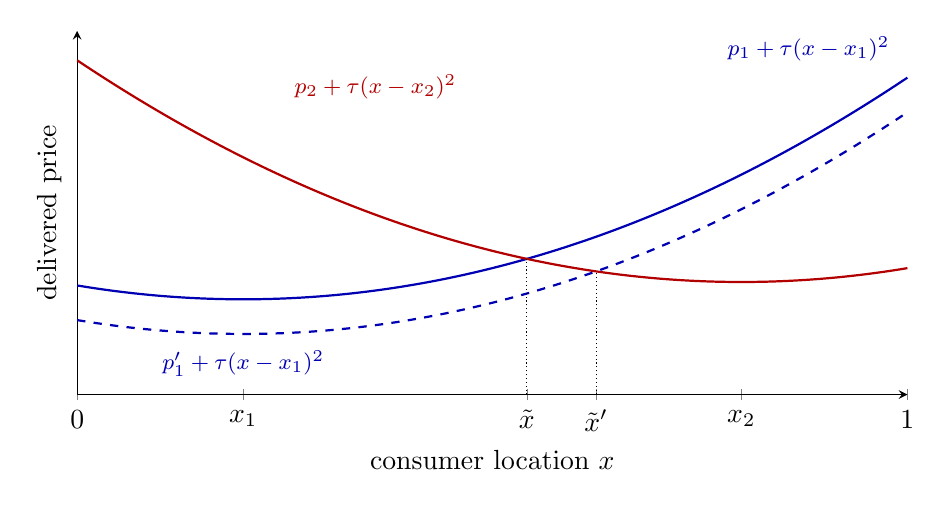
\begin{tikzpicture}
\begin{axis}[
  width=\linewidth, height=6.2cm,
  xmin=0, xmax=1, ymin=0.45, ymax=2.55,
  axis lines=left,
  xtick={0,0.2,0.5417,0.625,0.8,1},
  xticklabels={$0$,$x_1$,$\tilde x$,$\tilde x'$,$x_2$,$1$},
  ytick=\empty,
  xlabel={consumer location $x$},
  ylabel={delivered price},
  samples=201, domain=0:1,
  clip=false]
\addplot[thick, blue!70!black] {1 + 2*(x - 0.2)^2};
\addplot[thick, red!70!black] {1.1 + 2*(x - 0.8)^2};
\addplot[thick, dashed, blue!70!black] {0.8 + 2*(x - 0.2)^2};
\draw[densely dotted] (axis cs:0.5417,0.45) -- (axis cs:0.5417,1.234);
\draw[densely dotted] (axis cs:0.625,0.45) -- (axis cs:0.625,1.161);
\node[anchor=south west, font=\footnotesize, red!70!black] at (axis cs:0.25,2.1) {$p_2 + \tau(x - x_2)^2$};
\node[anchor=south east, font=\footnotesize, blue!70!black] at (axis cs:0.99,2.32) {$p_1 + \tau(x - x_1)^2$};
\node[anchor=north, font=\footnotesize, blue!70!black] at (axis cs:0.2,0.76) {$p_1' + \tau(x - x_1)^2$};
\end{axis}
\end{tikzpicture}
\caption{Quadratic transport costs}
\end{subfigure}
\caption{Delivered prices on Hotelling's line. Solid curves show each firm's price plus transport cost at the
initial prices, and the indifferent consumer $\tilde x$ is where they cross. In panel (a), with linear costs, firm 1
cuts its price to $p_1' = p_2 - \tau(x_2 - x_1)$ (dashed). Its schedule then coincides with firm 2's beyond $x_2$,
so firm 2's whole hinterland switches at once and demand jumps. In panel (b), with quadratic costs, a price cut (dashed)
moves the indifferent consumer continuously from $\tilde x$ to $\tilde x'$. Both panels use $x_1 = 0.2$ and $x_2 = 0.8$.
Panel (a) uses $\tau = 1$, $p_1 = p_2 = 1$ and $p_1' = 0.4$, and panel (b) uses $\tau = 2$, $p_1 = 1$, $p_2 = 1.1$ and
$p_1' = 0.8$.}
\label{fig:04-hotelling}
\end{figure}

\casehead{Firms at the ends} With $a = b = 0$, the middle case of \eqref{eq:04-hotelling-linear-demand} holds whenever
$|p_1 - p_2| \le \tau$. Firm 1 maximizes $(p_1 - c)M[\frac{1}{2} + \frac{p_2 - p_1}{2\tau}]$, a concave quadratic. Its
first-order condition is $\frac{1}{2} + \frac{p_2 - 2p_1 + c}{2\tau} = 0$, so the best response is
$p_1 = \frac{c + \tau + p_2}{2}$. Symmetry gives $p_1 = p_2 = c + \tau$, with $\tilde x = \frac{1}{2}$ and profits
$\frac{\tau M}{2}$. Undercutting to take the whole market requires $p_1 \le p_2 - \tau = c$, which earns nothing. The
markup equals the transport cost, so it vanishes as the products become perfect substitutes. This is the same
outcome as with quadratic costs at the ends (\cref{ex:06-hotelling}).

\casehead{Nonexistence when the firms are close} \Citet{Hotelling1929} argued that firms would cluster at the center
of the market, the \emph{principle of minimum differentiation}. \Citet{DAspremontGabszewiczThisse1979} showed that
the argument breaks down at the pricing stage. With linear costs, firms that are close have no pure-strategy price
equilibrium at all.

\begin{proposition}[Existence with linear transport costs]\label{prop:04-dgt}
Under \cref{ass:04-hotelling} with linear costs and $a, b \ge 0$, a pure-strategy price equilibrium exists if and only if
\begin{equation}\label{eq:04-dgt}
\Big(1 + \frac{a - b}{3}\Big)^2 \ge \frac{4}{3}(a + 2b)
\qquad\text{and}\qquad
\Big(1 + \frac{b - a}{3}\Big)^2 \ge \frac{4}{3}(b + 2a).
\end{equation}
When it exists, it is $p_1 = c + \tau(1 + \frac{a - b}{3})$ and $p_2 = c + \tau(1 + \frac{b - a}{3})$. With symmetric
locations, $a = b$, an equilibrium exists if and only if $a \le \frac{1}{4}$, and then $p_1 = p_2 = c + \tau$.
\end{proposition}

\begin{proof}
\emph{Step 1.} Any equilibrium lies in the middle region of \eqref{eq:04-hotelling-linear-demand}. Suppose firm 1
served the whole market, $p_1 < p_2 - \tau\Delta x$. Its profit is nonnegative only if $p_1 \ge c$. Firm 2 sells
nothing, yet it could charge any price in $(c, p_1 + \tau\Delta x)$, win some consumers and earn a positive profit.
That is a profitable deviation. The same argument rules out firm 2 serving everyone. At the boundary prices some
consumers are indifferent. Whichever way they break ties, one firm can gain by a small price change, so boundary
prices are not equilibria either.

\emph{Step 2.} In the middle region firm 1's profit is
$(p_1 - c)M[\frac{1 + a - b}{2} + \frac{p_2 - p_1}{2\tau}]$, a concave quadratic in $p_1$. Its first-order condition,
multiplied by $2\tau$, is $\tau(1 + a - b) + p_2 - 2p_1 + c = 0$. Firm 2's condition is symmetric:
\begin{equation*}
2p_1 - p_2 = c + \tau(1 + a - b), \qquad 2p_2 - p_1 = c + \tau(1 + b - a).
\end{equation*}
Adding twice the first equation to the second gives $3p_1 = 3c + \tau(3 + a - b)$, so
$p_1 = c + \tau(1 + \frac{a - b}{3})$, and by symmetry $p_2 = c + \tau(1 + \frac{b - a}{3})$. At these prices
$\tilde x = \frac{1 + a - b}{2} + \frac{b - a}{3} = \frac{3 + a - b}{6}$, and firm 1 earns
\begin{equation*}
\pi_1 = \tau\,\frac{3 + a - b}{3}\cdot M\,\frac{3 + a - b}{6} = \frac{M\tau}{2}\Big(1 + \frac{a - b}{3}\Big)^2 .
\end{equation*}
The candidate lies in the middle region if $|p_1 - p_2| = \frac{2\tau|a - b|}{3} < \tau\Delta x$. Take $a \ge b$. The
condition fails only if $5a + b \ge 3$, which with $b \le a$ requires $a \ge \frac{1}{2}$. Then the right side of
the second inequality in \eqref{eq:04-dgt} is at least $\frac{4}{3}$, while its left side is at most one. So
whenever \eqref{eq:04-dgt} holds, the candidate is interior.

\emph{Step 3.} Within the middle region the candidate is firm 1's best price. Prices that give firm 1 no
demand earn zero. The remaining deviation undercuts into the first region. There profit is $M(p_1 - c)$, which rises
with $p_1$, so the supremum is approached as $p_1$ rises to $p_2 - \tau\Delta x$. Its value is
\begin{equation*}
M\big(p_2 - \tau\Delta x - c\big) = M\tau\Big[1 + \frac{b - a}{3} - (1 - a - b)\Big] = \frac{2}{3}M\tau(a + 2b).
\end{equation*}
The candidate is a best response for firm 1 if and only if
$\frac{M\tau}{2}(1 + \frac{a - b}{3})^2 \ge \frac{2}{3}M\tau(a + 2b)$, which is the first inequality in
\eqref{eq:04-dgt}. The second inequality is the same condition for firm 2. By Steps 1 and 2 no other price pair
can be an equilibrium. With $a = b$ both inequalities read $1 \ge 4a$.
\end{proof}

The undercutting deviation drives the result. Holding firm 2's location fixed, firm 1's profit at the candidate
prices rises as firm 1 moves toward the center, with slope $\frac{M\tau}{3}(1 + \frac{a - b}{3})$. Its undercutting
payoff $\frac{2}{3}M\tau(a + 2b)$ rises faster, with slope $\frac{2}{3}M\tau$, and it also rises with $b$. When both
firms move inward together, $a = b$, the candidate profit stays at $\frac{M\tau}{2}$ while the undercutting payoff
$2M\tau a$ grows. When the firms are close, each prefers to undercut
the other and capture the whole line, and no pair of prices is stable. Mixed-strategy equilibria still exist, but
they are of little use for comparative statics (\cref{sec:04-existence-problem}). Hotelling's principle of minimum
differentiation therefore fails as a result about the location-price game. \Citet{CaplinNalebuff1991} make the same
point from the side of their existence theorem. Hotelling's distance utility is not linear in the consumer's
location, and the resulting discontinuity of demand is inconsistent with their assumptions (\cref{thm:04-cn-existence}).

\subsection{Quadratic transport costs and the location-price game}\label{sec:04-hotelling-quad}

\Citet{DAspremontGabszewiczThisse1979} restored existence by making transport costs quadratic. A consumer at $x$
then pays $p_j + \tau(x - x_j)^2$. The cost difference between the two firms is linear in $x$, so the
indifferent consumer moves continuously with prices, as panel (b) of \cref{fig:04-hotelling} shows. We now allow any
real $a$ and $b$ with $a + b < 1$, so that firms may also locate outside the line.

\begin{proposition}[Hotelling with quadratic costs]\label{prop:04-hotelling}
Let \cref{ass:04-hotelling} hold with quadratic costs and suppose that $|a - b| < 3$, so that the indifferent
consumer at the prices below lies strictly inside $[0,1]$.
\begin{enumerate}[label=(\roman*)]
\item The unique price equilibrium is
\begin{equation}\label{eq:04-hotelling-quad-prices}
p_1 = c + \tau(1 - a - b)\Big(1 + \frac{a - b}{3}\Big), \qquad p_2 = c + \tau(1 - a - b)\Big(1 + \frac{b - a}{3}\Big),
\end{equation}
with $q_1 = M\frac{3 + a - b}{6}$ and $\pi_1 = \frac{M\tau}{18}(1 - a - b)(3 + a - b)^2$.
\item In the first stage of a game in which firms choose locations and then prices,
\begin{equation}\label{eq:04-hotelling-location}
\frac{\dd\pi_1}{\dd a} = -\frac{M\tau}{18}(3 + a - b)(1 + 3a + b) < 0 \qquad\text{for all } a, b \ge 0 .
\end{equation}
If locations are restricted to $[0,1]$, the unique location equilibrium is $x_1 = 0$, $x_2 = 1$ (maximal
differentiation), with prices $c + \tau$.
\item If locations are unrestricted, the location equilibrium is $x_1 = -\frac{1}{4}$ and $x_2 = \frac{5}{4}$.
\end{enumerate}
\end{proposition}

\begin{proof}
(i) Let $\Delta x = 1 - a - b$. The indifferent consumer solves $p_1 + \tau(x - a)^2 = p_2 + \tau(x - 1 + b)^2$. The
quadratic terms $\tau x^2$ cancel, leaving
\begin{equation*}
2\tau x\,(1 - b - a) = p_2 - p_1 + \tau\big[(1 - b)^2 - a^2\big] = p_2 - p_1 + \tau(1 - a - b)(1 - b + a),
\end{equation*}
so that
\begin{equation*}
\tilde x = \frac{1 + a - b}{2} + \frac{p_2 - p_1}{2\tau\Delta x} = a + \frac{\Delta x}{2} + \frac{p_2 - p_1}{2\tau\Delta x}.
\end{equation*}
Consumers to the left of $\tilde x$ buy from firm 1, so $q_1 = M\tilde x$ when $\tilde x \in [0,1]$. Firm 1 maximizes
$(p_1 - c)M\tilde x$. Its first-order condition, multiplied by $\frac{2\tau\Delta x}{M}$, is
$\tau\Delta x(1 + a - b) + p_2 - 2p_1 + c = 0$. Firm 2 sells $M(1 - \tilde x)$ and has the symmetric condition.
The system is
\begin{equation*}
2p_1 - p_2 = c + \tau\Delta x(1 + a - b), \qquad 2p_2 - p_1 = c + \tau\Delta x(1 + b - a).
\end{equation*}
Adding twice the first to the second gives $3p_1 = 3c + \tau\Delta x(3 + a - b)$, which is
\eqref{eq:04-hotelling-quad-prices}. Then $p_2 - p_1 = \frac{2}{3}\tau\Delta x(b - a)$, so
$\tilde x = \frac{1 + a - b}{2} + \frac{b - a}{3} = \frac{3 + a - b}{6}$. Profit is
$(p_1 - c)M\tilde x = \tau\Delta x\frac{3 + a - b}{3}\cdot M\frac{3 + a - b}{6}$. Demand is continuous, and where
positive it is the minimum of $M$ and a linear function, hence log-concave. By \cref{lem:04-logconcave} profit is
quasi-concave in own price, so the first-order conditions give best responses, and the prices
\eqref{eq:04-hotelling-quad-prices} are an equilibrium.

The best-response map is not a contraction on all prices. When $p_2$ is high, firm 1's best response takes the
whole market, $\tilde x = 1$, and then rises one for one with $p_2$. We therefore prove uniqueness directly. In an
equilibrium with $0 < \tilde x < 1$, profits are differentiable in own prices, so both first-order conditions hold.
The linear system above then has the single solution \eqref{eq:04-hotelling-quad-prices}. Suppose instead that an
equilibrium had $\tilde x \geq 1$, so that firm 2 sells nothing. If $\tilde x > 1$, firm 1 could raise its price
slightly and still serve everyone, so $\tilde x = 1$. If $p_2 > c$, firm 2 could cut its price slightly and earn a
positive profit, so $p_2 \leq c$. With $\tilde x = 1$, firm 1's price is
$p_1 = p_2 - \tau\Delta x(1 - a + b) \leq c - \tau\Delta x(1 - a + b)$. A small rise in $p_1$ changes firm 1's
profit at the rate $M\big[1 - \frac{p_1 - c}{2\tau\Delta x}\big]$, so firm 1 gains from it unless
$p_1 - c \geq 2\tau\Delta x$. Both bounds on $p_1 - c$ hold only if $a - b \geq 3$, which the assumption rules out.
The case $\tilde x \leq 0$ is symmetric and requires $b - a \geq 3$. The equilibrium is therefore unique.

(ii) By the envelope theorem, the effect of $a$ on $\pi_1$ at the equilibrium of (i) has two parts. The direct
effect holds both prices fixed: $(p_1 - c)M\frac{\partial\tilde x}{\partial a}$. The strategic effect works through
the rival's price: $(p_1 - c)M\frac{\partial\tilde x}{\partial p_2}\frac{\dd p_2}{\dd a}$. Firm 1's own price response
has no first-order effect. At the equilibrium, with $\frac{p_2 - p_1}{2\tau\Delta x^2} = \frac{b - a}{3\Delta x}$,
\begin{equation*}
\frac{\partial\tilde x}{\partial a} = \frac{1}{2} + \frac{p_2 - p_1}{2\tau\Delta x^2} = \frac{3 - 5a - b}{6\Delta x},
\qquad
\frac{\partial\tilde x}{\partial p_2} = \frac{1}{2\tau\Delta x},
\qquad
\frac{\dd p_2}{\dd a} = -\frac{\tau(4 - 2a)}{3}.
\end{equation*}
The last derivative follows from differentiating $p_2 = c + \frac{\tau}{3}(1 - a - b)(3 + b - a)$, which gives
$\frac{\tau}{3}[-(3 + b - a) - (1 - a - b)] = -\frac{\tau}{3}(4 - 2a)$. Adding the two effects,
\begin{equation*}
\frac{\dd\pi_1}{\dd a} = (p_1 - c)M\Big[\frac{3 - 5a - b}{6\Delta x} - \frac{4 - 2a}{6\Delta x}\Big]
= -(p_1 - c)M\frac{1 + 3a + b}{6\Delta x}.
\end{equation*}
Substituting $p_1 - c = \frac{\tau\Delta x(3 + a - b)}{3}$ gives \eqref{eq:04-hotelling-location}, which is negative
for $a, b \ge 0$. Each firm therefore wants to move away from the center for any location of its rival. On $[0,1]$
the unique equilibrium is $a = b = 0$, and (i) gives prices $c + \tau$.

(iii) Without restrictions, the location first-order conditions are $1 + 3a + b = 0$ for firm 1 and
$1 + 3b + a = 0$ for firm 2. Their solution is $a = b = -\frac{1}{4}$, so $x_1 = -\frac{1}{4}$ and
$x_2 = 1 + \frac{1}{4} = \frac{5}{4}$. Given $b = -\frac{1}{4}$, the derivative \eqref{eq:04-hotelling-location} is
positive for $a < -\frac{1}{4}$ and negative above, so $a = -\frac{1}{4}$ is firm 1's best location.
\end{proof}

The two effects in the proof have a clear meaning. The direct effect is positive as long as $5a + b < 3$. Moving
toward the center at given prices takes consumers from the rival. The strategic effect is negative, because moving
closer makes the products better substitutes and lowers the rival's price. The strategic effect always wins.
\Citet{ShakedSutton1982} call this \emph{relaxing price competition through product differentiation}. Firms give up
market share at given prices to soften the price war that would follow. The result is
\emph{maximal differentiation}, the opposite of Hotelling's conjecture.

Equilibrium differentiation is excessive from the social point of view. With a covered market and inelastic unit
demand, prices are transfers, and welfare depends only on transport costs. A planner who places two products to
minimize average transport cost chooses $\frac{1}{4}$ and $\frac{3}{4}$, with average cost
$2\int_0^{\frac{1}{2}}\tau(x - \frac{1}{4})^2\dd x = \frac{\tau}{48}$. Firms at the ends impose
$2\int_0^{\frac{1}{2}}\tau x^2\dd x = \frac{\tau}{12}$, four times as much. When firms may locate outside the line, they move
even farther apart, to $-\frac{1}{4}$ and $\frac{5}{4}$. \Citet[Section 7.1.1]{Tirole1988} gives a textbook treatment.

\casehead{Minimal differentiation with fixed prices} Hotelling's principle does hold when prices cannot compete.
\Citet[Section 7.1.3]{Tirole1988} shows this with Hotelling's own location game at an exogenous price.

\begin{proposition}[Location choice at a fixed price]\label{prop:04-hotelling-fixed}
Let consumers be uniform on $[0,1]$ with mass $M$ and buy one unit each from the nearest firm. Two firms sell at a
common exogenous price $p > c$ and choose locations $x_1 = a$ and $x_2 = 1 - b$, splitting demand equally if they
locate at the same point. The unique equilibrium places both firms at $\frac{1}{2}$.
\end{proposition}

\begin{proof}
Prices and margins are fixed, so each firm maximizes its demand. Suppose first that $a < 1 - b$. Firm 1 serves its
hinterland and half of the consumers between the firms, so its demand is
\begin{equation*}
q_1 = M\Big[a + \frac{1 - b - a}{2}\Big] = M\,\frac{1 + a - b}{2} .
\end{equation*}
It rises with $a$, so firm 1 gains by moving toward its rival, and the same holds for firm 2. Any equilibrium therefore
has $a = 1 - b$. Suppose the common location is $x < \frac{1}{2}$. Each firm sells $\frac{M}{2}$. If firm 2 moves to
$x + e$ with small $e > 0$, it serves every consumer to the right of $x + \frac{e}{2}$, which gives
$M(1 - x - \frac{e}{2}) > \frac{M}{2}$. So $x < \frac{1}{2}$ is not an equilibrium, and the same argument rules out
$x > \frac{1}{2}$. At $x = \frac{1}{2}$, a firm that moves to any $x' \neq \frac{1}{2}$ serves only the consumers on
its side of the midpoint between $x'$ and $\frac{1}{2}$. That is less than half of the market, so neither firm
deviates.
\end{proof}

The products are socially too close. With linear costs, the average distance is $\frac{1}{4}$ when both firms sit
at the center and $\frac{1}{8}$ at the efficient locations $\frac{1}{4}$ and $\frac{3}{4}$. The contrast with
\cref{prop:04-hotelling} isolates the role of prices. Firms differentiate to soften price competition, and without
price competition they have no reason to. \citet[Section 7.1.3]{Tirole1988} groups the forces that work against
maximal differentiation into three categories. The first is the location of demand. Firms want to be where consumers
are, and when demand is concentrated around a few poles they cluster there. Tirole's examples are ice cream parlors
and bookstores near universities. The second is positive externalities among firms. On the cost side these include
shared installations and sources of raw materials. On the demand side, consumer search draws stores together, as
with the furniture stores of a single Paris street. The third is the absence of price competition, as in the game
above. Airline fares in the United States before deregulation and the prices of gasoline and books in France were
once set outside the market. Resale price maintenance has the same effect. Tirole adds that fixed-price location
models may explain why political platforms cluster at the center.

Two connections close this subsection. First, quadratic costs satisfy the linearity assumption of
\cref{thm:04-cn-existence}. Expanding the square gives $-\tau(x - x_j)^2 = -\tau x^2 + 2\tau x\,x_j - \tau x_j^2$. The
first term is common to all products and drops out, and the second is linear in the consumer's type $x$. With
uniform types, which have a log-concave density, an equilibrium exists for any locations
\citep{CaplinNalebuff1991}. Second, heterogeneity in tastes can bring minimum differentiation back.
\Citet{DePalmaEtAl1985} add a logit taste shock to Hotelling's linear transport costs. Demand becomes smooth, and with
enough taste heterogeneity relative to $\tau$, both firms locate at the center of the market. Their title states the
result: the principle of minimum differentiation holds under sufficient heterogeneity.

\subsection{Salop's circle, free entry and excess variety}\label{sec:04-salop}

\Citet{Salop1979} removed the ends of the line by placing consumers on a circle. Without ends there are no
hinterlands, and symmetric configurations with any number of firms are natural. This makes the circle the standard
model of entry with differentiated products.

\begin{proposition}[Salop's circle]\label{prop:04-salop}
Let a mass $M$ of consumers be uniform on a circle of circumference one, buy one unit each, and have a high enough
reservation value that the market is covered. $N$ firms are equally spaced, with marginal cost $c$, fixed cost
$\phi$ and linear transport cost $\tau$.
\begin{enumerate}[label=(\roman*)]
\item There is a symmetric price equilibrium with $p = c + \frac{\tau}{N}$, in which each firm earns
$\frac{\tau M}{N^2} - \phi$.
\item Treating $N$ as continuous, free entry yields $N^* = \sqrt{\frac{\tau M}{\phi}}$ firms.
\item The number of firms that minimizes fixed plus transport costs is $N^o = \frac{1}{2}\sqrt{\frac{\tau M}{\phi}}$.
Hence $N^* = 2N^o$.
\end{enumerate}
\end{proposition}

\begin{proof}
(i) Take a firm that charges $p$ while its two neighbors, each at distance $\frac{1}{N}$, charge $\bar p$. A consumer
at distance $d$ from the firm, on the arc toward a neighbor, is indifferent when
$p + \tau d = \bar p + \tau(\frac{1}{N} - d)$, that is, at $d = \frac{1}{2N} + \frac{\bar p - p}{2\tau}$. The firm serves
the arcs on both sides, so its demand is
\begin{equation*}
q = 2Md = M\Big[\frac{1}{N} + \frac{\bar p - p}{\tau}\Big] \qquad\text{for } |\bar p - p| \le \frac{\tau}{N}.
\end{equation*}
In this range profit $(p - c)q - \phi$ is a concave quadratic. Its first-order condition is
$\frac{1}{N} + \frac{\bar p - p}{\tau} - \frac{p - c}{\tau} = 0$. At a symmetric point $p = \bar p$, it gives
$p = c + \frac{\tau}{N}$. Each firm sells $\frac{M}{N}$ and earns $\frac{\tau}{N}\cdot\frac{M}{N} - \phi$. To take its
neighbor's whole market, a firm would have to price at $\bar p - \frac{\tau}{N} = c$, which earns no variable profit.
A price above $\bar p + \frac{\tau}{N}$ sells nothing. So no deviation outside the range is profitable.

(ii) Free entry drives profit to zero: $\frac{\tau M}{N^2} = \phi$, so $N^* = \sqrt{\frac{\tau M}{\phi}}$.

(iii) With $N$ equally spaced firms, each consumer travels to the nearest firm. Distances are uniform on
$[0, \frac{1}{2N}]$, so the average distance is $\frac{1}{4N}$ and total transport cost is $\frac{\tau M}{4N}$.
Prices are transfers because the market is covered. The planner minimizes $N\phi + \frac{\tau M}{4N}$. The
first-order condition $\phi - \frac{\tau M}{4N^2} = 0$ gives $N^o = \frac{1}{2}\sqrt{\frac{\tau M}{\phi}}$.
\end{proof}

\begin{figure}[htbp]
\centering
\begin{tikzpicture}
\def\R{2.3}
\draw[thick] (0,0) circle (\R);
\draw[line width=6pt, blue!25] (60:\R) arc (60:120:\R);
\foreach \a in {90,30,150,210,270,330} {\fill (\a:\R) circle (2.6pt);}
\foreach \a in {60,120} {\draw[thick] (\a:\R-0.18) -- (\a:\R+0.18);}
\node[anchor=south] at (90:\R+0.2) {firm $j$, price $p$};
\node[anchor=south west] at (30:\R+0.12) {firm $j+1$, price $\bar p$};
\node[anchor=south east] at (150:\R+0.12) {firm $j-1$, price $\bar p$};
\draw[<->, >=Stealth] (90:\R-0.55) arc (90:30:\R-0.55);
\node at (58:\R-1.05) {$\frac{1}{N}$};
\draw[<->, >=Stealth] (90:\R-1.0) arc (90:120:\R-1.0);
\node at (106:\R-1.45) {$\frac{1}{2N}$};
\node[align=center, font=\small] at (0,-0.45) {consumers uniform\\on the circle};
\end{tikzpicture}
\caption{Salop's circle with $N = 6$ equally spaced firms. Firm $j$ serves the shaded arc between the two
indifferent consumers (tick marks). At symmetric prices each indifferent consumer is at distance
$d = \frac{1}{2N}$ from firm $j$, so the firm's market has length $\frac{1}{N}$. A price cut by firm $j$ moves
both tick marks outward and takes customers from its two neighbors only.}
\label{fig:04-salop}
\end{figure}

\Cref{fig:04-salop} shows the structure. Each firm competes only with its two neighbors, and its markup
$\frac{\tau}{N}$ falls as the circle fills up. The market provides twice the efficient number of products. The reason
is the balance of two externalities \citep{Spence1976,DixitStiglitz1977,MankiwWhinston1986}. An entrant creates
variety: consumers near its location travel less. It does not capture this whole benefit in its profit, which pushes
toward too little entry. An entrant also steals business from incumbents, which pushes toward too much entry. On the
circle the market is covered, so every unit the entrant sells is taken from a rival. At $N^*$ the entrant's private
gain, its variable profit $\frac{\tau M}{N^2} = \phi$, is four times the social gain $\frac{\tau M}{4N^2} = \frac{\phi}{4}$
in saved transport costs. Business stealing dominates. \Cref{prop:02-mw-excess} gives the corresponding result for
homogeneous goods.

\begin{remark}[Coverage and touching markets]\label{rem:04-salop-coverage}
\Cref{prop:04-salop} assumes that every consumer buys. Let $\bar u$ be the reservation value. The consumer farthest
from a firm is at distance $\frac{1}{2N}$ and pays $c + \frac{\tau}{N} + \frac{\tau}{2N} = c + \frac{3\tau}{2N}$, so the
equilibrium requires $\bar u \ge c + \frac{3\tau}{2N}$. At free entry $\frac{\tau}{N^*} = \sqrt{\frac{\tau\phi}{M}}$, and
the condition becomes
\begin{equation*}
\frac{3}{2}\sqrt{\frac{\tau\phi}{M}} \le \bar u - c
\quad\Longleftrightarrow\quad
\phi \le \bar\phi = \frac{4M(\bar u - c)^2}{9\tau}
\end{equation*}
\citep[Section 7.1.2]{Tirole1988}. With larger fixed costs fewer firms enter, and the consumer halfway between two
firms would not buy at the price of the proposition. \Citet{Salop1979} studies this case. Suppose the neighbors charge
$\bar p = \bar u - \frac{\tau}{2N}$, so that the consumer halfway between two firms is just willing to buy. A firm that
raises its price loses customers to the outside good. Its demand is then $\frac{2M(\bar u - p)}{\tau}$, with slope
$-\frac{2M}{\tau}$. A firm that cuts its price takes customers from its neighbors, with the demand of the proof and
slope $-\frac{M}{\tau}$. Demand therefore has a kink at $\bar p$. At sales of $\frac{M}{N}$, a price rise does not pay if
$\frac{M}{N} \le \frac{2M}{\tau}(\bar p - c)$, and a price cut does not pay if $\frac{M}{N} \ge \frac{M}{\tau}(\bar p - c)$.
So $\bar p$ is an equilibrium price whenever
\begin{equation*}
\frac{\tau}{N} \le \bar u - c \le \frac{3\tau}{2N} .
\end{equation*}
Free entry requires $G(N) \equiv (\bar u - c - \frac{\tau}{2N})\frac{M}{N} = \phi$. In this regime
$G'(N) = \frac{M}{N^2}\big[\frac{\tau}{N} - (\bar u - c)\big] \le 0$, and $G$ also falls with $\tau$. A higher fixed cost
or a higher transport cost therefore lowers the number of firms, and the price $\bar u - \frac{\tau}{2N}$ falls with it.
In the competitive regime of the proposition both changes raise the price. \Citet[Section 7.1.2,
Exercise 7.4]{Tirole1988} calls such results a priori counterintuitive. The explanation is that the price is pinned
by the reservation value of the consumer halfway between two firms. When firms are farther apart, that consumer
travels farther and can pay less.
\end{remark}

The factor of two depends on linear costs. With quadratic costs $\tau d^2$ on the circle, the same steps give the
markup $\frac{\tau}{N^2}$ and free-entry number $N^* = (\frac{\tau M}{\phi})^{\frac{1}{3}}$. Average transport cost is
$\frac{\tau}{12N^2}$, so the optimum is $N^o = (\frac{\tau M}{6\phi})^{\frac{1}{3}}$ and $\frac{N^*}{N^o} = 6^{\frac{1}{3}} \approx 1.82$.
Entry is still excessive. The dimension of the space matters more. \Citet{CaplinNalebuff1991} discuss
\citet{Stiglitz1986}, who places firms on a grid in $L$ dimensions with quadratic transport costs, so each firm has
$2L$ neighbors. Demand becomes more elastic as $L$ grows, profits fall, and fewer firms can cover the entry cost.
Yet consumers have farther to travel in higher dimensions, so the efficient number of firms per unit area rises.
Stiglitz concludes that low-dimensional markets have excess diversity and high-dimensional markets too little
\citep[Section 8.3 and n.~21]{CaplinNalebuff1991}. Caplin and Nalebuff show that, with quadratic costs, the
symmetric solution of the first-order conditions in his model is indeed an equilibrium. \Cref{fig:04-voronoi}
shows the two-dimensional analogue of the circle's market areas.

The circle fixes locations by assumption. \Citet[Section 7.1.2]{Tirole1988} discusses three extensions. First, equal
spacing is a natural guess given maximal differentiation on the line. \Citet{Economides1989} justifies it with
quadratic costs in a game where firms choose entry, then locations, then prices, and a symmetric free-entry
equilibrium exists. Tirole cites the 1984 working-paper version. Second, firms may enter in sequence, and then an
early entrant's location shapes later choices. \Citet{PrescottVisscher1977} studied sequential location on the line.
Third, one firm may sell several brands and crowd the product space so that no entrant fits, especially when it can
preempt. \Citet[p.~1283, n.~4]{AndersonDePalmaNesterov1995} add that the known results for the circle all suggest
substantial overentry at every level of fixed costs.

The welfare comparison has been taken to data. \Citet{BerryWaldfogel1999} estimate how listening and advertising
revenue vary with the number of radio stations in 135 US metropolitan markets and recover fixed costs from a
free-entry condition. In the 1996 working-paper version on which we rely, the welfare loss from free entry relative
to the social optimum is 40 percent of industry revenue. This calculation leaves out the value of programming to
listeners. Advertisers pay 4.5 cents per hour for a marginal listener. The authors compute that free entry would be
optimal if programming were worth more than three times that amount to the marginal listener.

\subsection{Symmetric logit oligopoly and entry*}\label{sec:04-logit-entry}

The symmetric logit gives a useful contrast with the circle. Every product competes with every other, and each new
product brings a new taste shock and hence new variety.

\begin{proposition}[Symmetric logit oligopoly and entry]\label{prop:04-logit-entry}
Let $N \ge 2$ single-product firms sell products with common quality $\tilde\delta$ and marginal cost $c$ to a mass
$M$ of consumers with logit demand and no outside good. Each firm pays a fixed cost $\phi$.
\begin{enumerate}[label=(\roman*)]
\item The symmetric price equilibrium has markup $p - c = \frac{N}{\alpha(N - 1)}$, and each firm earns
$\frac{M}{\alpha(N - 1)} - \phi$. With an outside good, the markup is $\frac{1}{\alpha(1 - s)}$, with $s$ each
firm's share.
\item Treating $N$ as continuous, free entry yields $N^* = 1 + \frac{M}{\alpha\phi}$.
\item Total surplus is $TS(N) = \frac{M}{\alpha}\ln N + M\big(\frac{\tilde\delta}{\alpha} - c\big) - N\phi$, up to a
constant. It is maximized at $N^o = \frac{M}{\alpha\phi}$, so $N^* = N^o + 1$.
\end{enumerate}
\end{proposition}

\begin{proof}
(i) With no outside good, the shares are $\frac{e^{\delta_j}}{\sum_ke^{\delta_k}}$, and at symmetric prices $s = \frac{1}{N}$.
The first-order condition of a single-product firm, $\alpha(p - c)(1 - s) = 1$, is derived as in
\cref{prop:04-logit-markup}, which does not use the outside good. With $s = \frac{1}{N}$ it gives
$p - c = \frac{1}{\alpha(1 - \frac{1}{N})} = \frac{N}{\alpha(N - 1)}$. Each firm sells $\frac{M}{N}$ and earns
$\frac{N}{\alpha(N-1)}\cdot\frac{M}{N} - \phi$. With an outside good, \cref{prop:04-logit-markup} applies directly.
(ii) Setting profit to zero gives $\alpha(N - 1)\phi = M$.
(iii) By \cref{prop:04-logit-entropy}, consumer surplus is $\frac{M}{\alpha}\ln\sum_{k=1}^Ne^{\tilde\delta - \alpha p}$ up
to a constant. At symmetric prices this equals $\frac{M}{\alpha}\ln N + \frac{M\tilde\delta}{\alpha} - Mp$. Total
profit is $M(p - c) - N\phi$. In the sum the price cancels, because every consumer buys and payments are
transfers. The derivative $TS'(N) = \frac{M}{\alpha N} - \phi$ vanishes at $N^o = \frac{M}{\alpha\phi}$, and $TS$ is
concave. Comparing with (ii) gives $N^* = N^o + 1$.
\end{proof}

The logit market also has too many products, but only one too many. The relative excess
$\frac{N^* - N^o}{N^o} = \frac{\alpha\phi}{M}$ vanishes as the market grows, whereas on the circle it is always
100 percent. The reason lies in the social value of the marginal product. In the logit it is $\frac{M}{\alpha N}$,
which falls slowly with $N$, because each product brings its own taste shock. On the circle it is
$\frac{\tau M}{4N^2}$, which falls fast, because a new product only shortens the trips of nearby consumers. The
entrant's private gain, $\frac{M}{\alpha(N - 1)}$, exceeds the social gain by only
$\frac{M}{\alpha N(N - 1)}$. Business stealing is weak because the logit treats variety itself as valuable.
\Citet[p.~49]{MankiwWhinston1986} isolate the two forces at work. Business stealing pushes toward excessive entry,
as in homogeneous-good markets. Product diversity pushes the other way, because the entrant creates surplus through
variety that it does not capture as profit. With the CES form and equilibrium notion of \citet{Spence1976}, the
diversity effect always dominates and entry is insufficient. They also give examples in which business stealing
always dominates. The symmetric logit of \cref{prop:04-logit-entry} is another such case, with an excess of one firm.
For the CES, \citet{DixitStiglitz1977} show that the market can provide too few or too many products, depending on
preferences (\cref{sec:04-repcons-monocomp}).

\casehead{General i.i.d.\ tastes} \Citet{AndersonDePalmaNesterov1995} ask how far the logit's verdict extends. They
keep the symmetric discrete choice structure, with the demand side of \citet{PerloffSalop1985}, but let the taste
shocks have any log-concave density. The following proposition collects the pieces we need, in our notation.

\begin{proposition}[Symmetric oligopoly with i.i.d.\ tastes]\label{prop:04-adn}
A mass $M$ of consumers each buy one unit of the product that maximizes $u_{ij} = y - p_j + \epsilon_{ij}$. The shocks
$\epsilon_{ij}$ are i.i.d.\ across consumers and products, with density $f_\epsilon$ and distribution function $F_\epsilon$
on $(\underline e, \bar e)$ and a finite mean. There are $N \ge 2$ single-product firms with marginal cost $c$ and
fixed cost $\phi$.
\begin{enumerate}[label=(\roman*)]
\item Demand for product $i$ is
\begin{equation}\label{eq:04-adn-demand}
q_i = M\int f_\epsilon(x)\prod_{j \ne i}F_\epsilon(p_j - p_i + x)\,\dd x .
\end{equation}
\item The unique candidate for a symmetric equilibrium has the markup
\begin{equation}\label{eq:04-adn-markup}
p - c = \frac{1}{\Theta(N)}, \qquad \Theta(N) = N(N - 1)\int f_\epsilon(x)^2F_\epsilon(x)^{N-2}\,\dd x .
\end{equation}
\item At equal prices, an $(N+1)$th product raises total surplus by $M\int F_\epsilon(x)^N[1 - F_\epsilon(x)]\,\dd x - \phi$.
Its profit in the symmetric equilibrium with $N + 1$ firms is $\frac{M}{(N + 1)\Theta(N + 1)} - \phi$.
\item If $\epsilon_{ij}$ is type-I extreme value with scale $\frac{1}{\alpha}$, then $\Theta(N) = \frac{\alpha(N - 1)}{N}$,
the markup is $\frac{N}{\alpha(N - 1)}$, and the surplus gain in (iii) is $\frac{M}{\alpha}\ln\frac{N + 1}{N} - \phi$.
\item If $F_\epsilon(x) = 1 - e^{-\lambda_\epsilon(x - \underline e)}$ on $[\underline e, \infty)$ with $\lambda_\epsilon > 0$,
then $\Theta(N) = \lambda_\epsilon$ for every $N$. The surplus gain and the profit in (iii) are both
$\frac{M}{\lambda_\epsilon(N + 1)} - \phi$.
\end{enumerate}
\end{proposition}

\begin{proof}
(i) Fix a consumer and write $\epsilon_k$ for her shock on product $k$. She buys $i$ when
$y - p_i + \epsilon_i > y - p_j + \epsilon_j$ for every $j \ne i$. Given $\epsilon_i = x$, this requires
$\epsilon_j < p_j - p_i + x$ for every $j \ne i$. By independence the conditional probability is
$\prod_{j \ne i}F_\epsilon(p_j - p_i + x)$. Integrating over the density of $x$ gives \eqref{eq:04-adn-demand}. Ties
have probability zero.

(ii) Differentiate \eqref{eq:04-adn-demand} with respect to $p_i$ and set all prices equal. Each of the $N - 1$ factors
contributes $-f_\epsilon(x)F_\epsilon(x)^{N-2}$, so
\begin{equation*}
\frac{\partial q_i}{\partial p_i} = -M(N - 1)\int f_\epsilon(x)^2F_\epsilon(x)^{N-2}\,\dd x = -\frac{M\,\Theta(N)}{N} .
\end{equation*}
At equal prices $q_i = \frac{M}{N}$. The first-order condition $q_i + (p_i - c)\frac{\partial q_i}{\partial p_i} = 0$
becomes $\frac{M}{N} = (p - c)\frac{M\,\Theta(N)}{N}$, which has the single solution \eqref{eq:04-adn-markup}.

(iii) Every consumer buys and prices are transfers, so at equal prices total surplus is $M(y - c)$ plus
$M\E[\max_j\epsilon_{ij}]$ minus total fixed costs. The maximum of $N$ shocks has distribution function $F_\epsilon^N$.
Integrating by parts, with boundary terms that vanish because the mean is finite,
\begin{equation*}
\E\big[\max_{j \le N + 1}\epsilon_{ij}\big] - \E\big[\max_{j \le N}\epsilon_{ij}\big]
= \int x\,\dd\big(F_\epsilon^{N+1} - F_\epsilon^N\big)(x) = \int F_\epsilon(x)^N\big[1 - F_\epsilon(x)\big]\,\dd x .
\end{equation*}
With $N + 1$ firms, each sells $\frac{M}{N + 1}$ at the markup $\frac{1}{\Theta(N + 1)}$, which gives the profit.

(iv) Here $F_\epsilon(x) = \exp(-e^{-\alpha x})$ and $f_\epsilon(x) = \alpha e^{-\alpha x}F_\epsilon(x)$, so
$f_\epsilon^2F_\epsilon^{N-2} = \alpha^2e^{-2\alpha x}\exp(-Ne^{-\alpha x})$. Substitute $u = e^{-\alpha x}$, with
$\dd x = -\frac{\dd u}{\alpha u}$:
\begin{equation*}
\int f_\epsilon(x)^2F_\epsilon(x)^{N-2}\,\dd x = \alpha\int_0^\infty ue^{-Nu}\,\dd u = \frac{\alpha}{N^2},
\qquad\text{so}\qquad
\Theta(N) = \frac{\alpha(N - 1)}{N} .
\end{equation*}
For the surplus, $F_\epsilon(x)^N = \exp\big(-e^{-\alpha(x - \frac{\ln N}{\alpha})}\big)$. The maximum of $N$ shocks is
therefore extreme value with location $\frac{\ln N}{\alpha}$, and its mean rises by $\frac{1}{\alpha}\ln\frac{N + 1}{N}$
when $N$ rises by one.

(v) Let $v = F_\epsilon(x)$, so that $f_\epsilon(x) = \lambda_\epsilon(1 - v)$ and $\dd v = \lambda_\epsilon(1 - v)\,\dd x$. Then
\begin{equation*}
\int f_\epsilon^2F_\epsilon^{N-2}\,\dd x = \lambda_\epsilon\int_0^1(1 - v)v^{N-2}\,\dd v
= \lambda_\epsilon\Big[\frac{1}{N - 1} - \frac{1}{N}\Big] = \frac{\lambda_\epsilon}{N(N - 1)},
\end{equation*}
so $\Theta(N) = \lambda_\epsilon$. Likewise $\int F_\epsilon^N(1 - F_\epsilon)\,\dd x = \frac{1}{\lambda_\epsilon}\int_0^1v^N\,\dd v =
\frac{1}{\lambda_\epsilon(N + 1)}$, and the profit is $\frac{M}{(N + 1)\lambda_\epsilon} - \phi$.
\end{proof}

Part (iv) is the integer version of \cref{prop:04-logit-entry}. The $(N+1)$th product adds
$\frac{M}{\alpha}\ln(1 + \frac{1}{N})$ to surplus and earns $\frac{M}{\alpha N}$, and $\ln(1 + \frac{1}{N}) < \frac{1}{N}$.
The general results of \citet{AndersonDePalmaNesterov1995} rest on log-concavity. Utility is linear in the vector of
shocks, whose joint density $\prod_jf_\epsilon(\epsilon_{ij})$ is log-concave when $f_\epsilon$ is. The theorem of
\citet{CaplinNalebuff1991} then makes profit quasi-concave, so the candidate in (ii) is an equilibrium (p.~1285,
\cref{thm:04-cn-existence}). Their Proposition 1 (p.~1285) shows that log-concavity also makes $\Theta(N)$
nondecreasing, so markups do not rise with entry. Revenue per firm then falls with $N$, and the free-entry number of
firms is unique. Their Theorem 1 (p.~1287) is the main result. With log-concave tastes and unit demands, the profit of
an extra firm is never below its social value, so the market never provides too little variety. Corollary 1
(p.~1289) shows that equilibrium and optimum coincide for every fixed cost only for the exponential-tail
distributions of part (v) and their mirror images. For the densities of their example held fixed, the equilibrium
number of firms is about the optimum plus one as fixed costs vanish (p.~1290), as in the logit. For a general fixed
density only the ratio of the two numbers tends to one, a result \citet[p.~1283]{AndersonDePalmaNesterov1995}
credit to \citet{DeneckereRothschild1992}. Overentry can still be large. For
each optimal number of firms they choose a log-concave density, and as fixed costs vanish the ratio of the
equilibrium to the optimal number tends to $r^* > 1.097$ (p.~1290). That is almost 10 percent excess entry even with
very many firms. When individual demand responds to price, entry can fall short of the optimum subject to zero
profits, but by at most one firm (their Theorem 2, p.~1294).

The logit's verdict depends on taking the taste shocks literally. If they are a statistical device, the term
$\frac{M}{\alpha}\ln N$ overstates the value of variety, and the true optimum may be far below $N^o$. This is the
``too many characteristics'' problem of \cref{sec:04-spaces-drawbacks} in its welfare form. It is also why models of
entry and variety that use logit demand need care before their welfare conclusions are trusted.

\subsection{Vertical differentiation and quality choice}\label{sec:04-vertical-quality}

In the models so far consumers disagree about which product is best at equal prices. In a \emph{vertical} model
they agree: at equal prices every consumer ranks products the same way. Consumers differ only in how much they value
quality relative to money. Consumer $i$ has utility $v_ix_j - p_j$ from product $j$ with quality $x_j$. The taste for
quality $v_i$ is uniform on $[\underline v, \bar v]$ with mass $M$. Dividing utility by $v_i$ gives
$x_j - \frac{1}{v_i}p_j$, the vertical model $u_{ij} = \delta_j - \nu_ip_j$ of \cref{ch:discrete} with
$\delta_j = x_j$ and price sensitivity $\nu_i = \frac{1}{v_i}$.

\begin{proposition}[Price and quality competition with vertical differentiation]\label{prop:04-vertical}
Two firms with a common marginal cost $c \ge 0$ sell qualities $x_1 < x_2$. Assume $\bar v > 2\underline v$ and the
coverage condition $c + \frac{1}{3}(\bar v - 2\underline v)(\bar x - \underline x) \le \underline v\,\underline x$, where
qualities lie in $[\underline x, \bar x]$.
\begin{enumerate}[label=(\roman*)]
\item The price equilibrium is
\begin{equation}\label{eq:04-vertical-prices}
p_1 = c + \frac{(\bar v - 2\underline v)(x_2 - x_1)}{3}, \qquad p_2 = c + \frac{(2\bar v - \underline v)(x_2 - x_1)}{3},
\end{equation}
with cutoff type $\hat v = \frac{\bar v + \underline v}{3}$ and profits
$\pi_1 = \frac{M(\bar v - 2\underline v)^2(x_2 - x_1)}{9(\bar v - \underline v)}$ and
$\pi_2 = \frac{M(2\bar v - \underline v)^2(x_2 - x_1)}{9(\bar v - \underline v)}$.
\item If firms first choose qualities in $[\underline x, \bar x]$ at no cost and then set prices, the equilibrium
qualities are $\underline x$ and $\bar x$.
\end{enumerate}
\end{proposition}

\begin{proof}
(i) Let $\Delta x = x_2 - x_1$. Type $v$ prefers quality 2 when $vx_2 - p_2 > vx_1 - p_1$, that is, when
$v > \hat v = \frac{p_2 - p_1}{\Delta x}$. Under coverage every type buys, so with density $\frac{M}{\bar v - \underline v}$,
\begin{equation*}
q_1 = M\frac{\hat v - \underline v}{\bar v - \underline v}, \qquad q_2 = M\frac{\bar v - \hat v}{\bar v - \underline v}.
\end{equation*}
Firm 1 maximizes $(p_1 - c)q_1$. Since $\frac{\partial\hat v}{\partial p_1} = -\frac{1}{\Delta x}$, its first-order
condition is $\hat v - \underline v - \frac{p_1 - c}{\Delta x} = 0$, or $p_2 - 2p_1 = \underline v\Delta x - c$. Firm 2's
condition is $\bar v - \hat v - \frac{p_2 - c}{\Delta x} = 0$, or $2p_2 - p_1 = \bar v\Delta x + c$. The first gives
$p_2 = 2p_1 + \underline v\Delta x - c$. Substituting into the second gives $3p_1 = 3c + (\bar v - 2\underline v)\Delta x$,
and then $p_2 = c + \frac{(2\bar v - \underline v)\Delta x}{3}$. The cutoff is
$\hat v = \frac{p_2 - p_1}{\Delta x} = \frac{\bar v + \underline v}{3}$, which lies strictly inside $(\underline v, \bar v)$
because $\bar v > 2\underline v$. Profits follow from the margins $p_j - c$ and from
$\hat v - \underline v = \frac{\bar v - 2\underline v}{3}$ and $\bar v - \hat v = \frac{2\bar v - \underline v}{3}$. Coverage
requires that the lowest type buy, $\underline vx_1 \ge p_1$. The left side is smallest and the right side largest at
$x_1 = \underline x$ and $x_2 = \bar x$, where the assumed condition makes it hold. A firm that raised its price
enough to lose low types would face demand no larger than the covered formula, so the candidate remains optimal.

(ii) Both profits are proportional to $\Delta x$. Given $x_2 = \bar x$, the low-quality firm's profit
$\propto \bar x - x_1$ is largest at $x_1 = \underline x$. Choosing $x_1 = \bar x$ would make the products identical and
drive both prices to marginal cost, and leapfrogging is impossible. Given $x_1 = \underline x$, the high-quality firm's
profit $\propto x_2 - \underline x$ is largest at $\bar x$. So $(\underline x, \bar x)$ is an equilibrium. In any
configuration with $\underline x < x_1$ or $x_2 < \bar x$, one firm can raise $\Delta x$ and its profit, and equal
qualities yield zero profits. So the only equilibria assign $\underline x$ to one firm and $\bar x$ to the other.
\end{proof}

\begin{figure}[htbp]
\centering
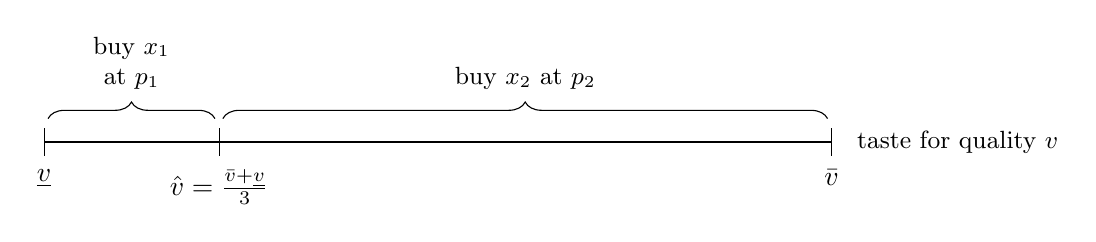
\begin{tikzpicture}[x=1cm,y=1cm]
\draw[thick] (0,0) -- (10,0);
\draw (0,0.18) -- (0,-0.18);
\draw (10,0.18) -- (10,-0.18);
\draw (2.222,0.18) -- (2.222,-0.18);
\node[below] at (0,-0.22) {$\underline v$};
\node[below] at (10,-0.22) {$\bar v$};
\node[below] at (2.222,-0.22) {$\hat v = \frac{\bar v + \underline v}{3}$};
\draw[decorate, decoration={brace, amplitude=6pt}] (0.05,0.3) -- (2.17,0.3)
  node[midway, above=7pt, align=center, font=\small] {buy $x_1$\\at $p_1$};
\draw[decorate, decoration={brace, amplitude=6pt}] (2.27,0.3) -- (9.95,0.3)
  node[midway, above=7pt, align=center, font=\small] {buy $x_2$ at $p_2$};
\node[anchor=west, font=\small] at (10.2,0) {taste for quality $v$};
\end{tikzpicture}
\caption{Market segments in the vertical duopoly of \cref{prop:04-vertical}, drawn for $\underline v = 1$ and
$\bar v = 4$. Consumers with a high taste for quality buy the high-quality product. The cutoff
$\hat v = \frac{\bar v + \underline v}{3}$ does not depend on the two qualities.}
\label{fig:04-vertical}
\end{figure}

\Cref{fig:04-vertical} shows the segments. The force behind part (ii) is the one we saw on Hotelling's line. Closer
qualities mean fiercer price competition, so firms differentiate as much as they can
\citep{GabszewiczThisse1979,ShakedSutton1982}. The high-quality firm charges more, sells more and earns more. Both
markups and profits scale with the quality gap $x_2 - x_1$, and they vanish when the products are identical.

\Citet[Section 7.5.1]{Tirole1988} draws out two further points. First, part (ii) has two equilibria, which differ
only in which firm takes the top quality. If one firm chooses its quality first, it takes $\bar x$ and leaves
$\underline x$ to its rival, so the equilibrium is unique. Since $\pi_2 > \pi_1$, each firm would like to move first.
With a cost of introducing a quality and growing demand, this becomes a preemption race, in which firms trade the
gain from leadership against the cost of entering too early. Second, maximal differentiation is not robust. If the
lowest feasible quality is so low that the coverage condition fails, the low-quality firm loses the bottom of the
market and no longer wants the lowest quality. The effect is stronger when marginal costs differ across qualities,
which already softens price competition. The principle of differentiation itself survives.

\begin{remark}[Natural oligopoly]\label{rem:04-natural-oligopoly}
The condition $\bar v > 2\underline v$ requires enough dispersion in tastes. If $\bar v \le 2\underline v$, formula
\eqref{eq:04-vertical-prices} would give $p_1 \le c$. The equilibrium then has $p_1 = c$ and the high-quality firm
serving every consumer at the limit price $p_2 = c + \underline v(x_2 - x_1)$, the highest price at which the lowest
type still prefers quality 2. To see this, write $m_2 = p_2 - c$. At $p_1 = c$, firm 2's profit for
$m_2 > \underline v\Delta x$ is $m_2M\frac{\bar v\Delta x - m_2}{(\bar v - \underline v)\Delta x}$. Its slope at
$m_2 = \underline v\Delta x$ is $M\frac{\bar v - 2\underline v}{\bar v - \underline v} \le 0$, and it is concave, so firm 2
does not raise its price further. With any positive fixed cost, only one firm enters, however large $M$ is. This is
the simplest instance of the finiteness property of \citet{ShakedSutton1983}, which \citet[Section 7.5.1]{Tirole1988}
states as follows. Let quality $x$ cost $c(x)$ per unit. Suppose that, if every quality were sold at its unit cost,
all consumers would buy the highest quality. Then at most a finite number of firms can have positive market shares,
whatever the relative sizes of demand and entry costs. Price competition among the high-quality firms leaves no room
for low qualities. The condition requires unit cost to rise slowly with quality. Shaked and Sutton therefore expect
finiteness when the burden of quality improvement falls mainly on research and development or other fixed costs,
rather than on labor and materials. On the circle, by contrast, the number of firms grows without bound as fixed
costs vanish. \Cref{ch:discrete} estimates the vertical demand model, and \citet{Bresnahan1987} applies it to the 1955
automobile price war.
\end{remark}

\subsection{From address models to discrete choice}\label{sec:04-location-bridge}

Location models are characteristics-space models with one or two characteristics and no idiosyncratic taste
shock. Substitution is local. On the line and the circle a product competes only with its neighbors, and in the
vertical model only with the products just above and below it in quality. Adding a product close to an existing one
adds little value, since the gain on the circle is the saved transport cost of nearby consumers. Logit-type models
sit at the opposite extreme. Every product competes with every other, IIA holds, and each new product adds value
through its own taste shock (\cref{sec:04-spaces-drawbacks}). The two classes share a formal structure.
Expanding the square in a quadratic ideal-point model turns it into a random coefficients model, as shown in
\cref{prop:06-idealpoint}. The pure characteristics model of \citet{BerryPakes2007} keeps the local substitution of
address models while allowing many characteristics and estimation from market data (\cref{ch:discrete}). Random
coefficient logit models (\cref{ch:blp}) sit between the extremes. They generate local substitution through
correlated tastes while keeping the logit shock.

Location models also frame empirical work on product choice. In the location and quality games above, firms choose
positions in anticipation of price competition. Mergers change these incentives. \Citet{Sweeting2010} studies how
radio stations reposition their formats after mergers (\cref{ch:mergers}). The estimation of such product choice
models builds on the equilibrium theory of this section.


\section{Bibliographic notes}\label{sec:04-notes}

\citet[ch.~7]{Tirole1988} and \citet{Vives1999} give textbook treatments of price competition with differentiated
products, and \citet{AndersonDePalmaThisse1992} build the theory on discrete choice. Tirole treats the linear city in
Section 7.1.1, the circular city in Section 7.1.2 and the forces for and against differentiation in Section 7.1.3.
Vertical differentiation is in Section 7.5.1, and monopolistic competition is in Sections 7.2 and 7.5.2. The location
tradition starts with \citet{Hotelling1929}. \citet{DAspremontGabszewiczThisse1979} overturned its conclusion about
minimum differentiation, and \citet{Salop1979} moved the model to the circle. \citet{Economides1989} studies location
choice on the circle, and \citet{PrescottVisscher1977} study sequential location on the line.
\citet{GabszewiczThisse1979} and \citet{ShakedSutton1982,ShakedSutton1983} developed vertical differentiation and the
theory of natural oligopoly.

\citet{Chamberlin1933} introduced monopolistic competition. The representative-consumer CES model of
\citet{Spence1976} and \citet{DixitStiglitz1977} remains its workhorse and that of trade theory
\citep{Krugman1980,Melitz2003}. \citet{MankiwWhinston1986} isolate the business-stealing and product-diversity
externalities behind excess or insufficient entry, and \citet{BerryWaldfogel1999} measure them in radio
broadcasting. \citet{PerloffSalop1985} replaced the representative consumer by a population with i.i.d.\ tastes for
the brands. \citet{AndersonDePalmaNesterov1995} use that model to show that log-concave tastes rule out
insufficient variety when each consumer buys one unit. With price-sensitive individual demand, the shortfall relative
to the zero-profit constrained optimum is at most one product.

\citet{CaplinNalebuff1991} remains the reference on existence of price equilibrium with single-product firms, and
\citet{Dierker1989} reached related conditions independently. The theory of supermodular games
\citep{MilgromRoberts1990,Vives1990} explains why log-supermodular price games are well behaved. Classical sufficient
conditions for uniqueness go back to \citet{Friedman1977} and \citet{GaleNikaido1965}.
\citet[Theorems~7 and~13]{KonovalovSandor2010} prove existence and uniqueness of price equilibrium with multi-product
firms for the simple logit and for CES demand.
\citet{NockeSchutz2018} develop an aggregative-games approach to multi-product price competition with logit and CES
demands. Each firm's profit depends on its rivals' prices only through a one-dimensional aggregator, and firms may
differ in their numbers of products \citep[p.~229, n.~127, and p.~232, n.~140]{AskerNocke2021}.

The multi-product pricing equation became a standard part of empirical work with \citet{Berry1994} and
\citet{BerryLevinsohnPakes1995}, who used it to recover costs and to sharpen demand estimates. \citet{Bresnahan1987}
and \citet{Nevo2001} used it to compare models of conduct. \citet{BerryHaile2014} formalize the identification of
conduct with differentiated products, and \citet{BackusConlonSinkinson2021} and \citet{DuarteEtAl2024} develop tests
among conduct models. Profit weights from partial ownership go back to \citet{OBrienSalop2000}, and
\citet{MillerWeinberg2017} estimate a weight for a joint venture. \citet{FarrellShapiro2010} put diversion ratios at
the center of merger screening, and \citet{ConlonMortimer2021} study how to measure them. \citet{MorrowSkerlos2011}
provide a fixed-point algorithm that computes equilibria reliably with mixed logit demand, and \citet{Werden1996}
derives the cost reductions that leave prices unchanged after a merger.

The characteristics approach goes back to \citet{Lancaster1966} and \citet{Gorman1980}, and \citet{McFadden1974}
gave it its econometric form. \citet{McFadden1984} surveys the qualitative response models that implement it, and
\citet{BerryPakes2007} analyze the pure characteristics model, which drops the product-specific taste shock.
\citet{DeatonMuellbauer1980a} is the standard reference for demand systems in product space (\cref{ch:aids}).
\citet{Hausman1997} argues that symmetric systems such as the logit and the CES overstate the value of new goods, a
theme that \cref{ch:newgoods} takes up.

\section{Exercises}\label{sec:04-exercises}

\begin{enumerate}[label=\arabic*., leftmargin=*, itemsep=6pt]

\item \textit{Asymmetric costs, upward pricing pressure and cost-reducing investment.} Let demands be $q_1 = a - bp_1 + dp_2$ and
$q_2 = a - bp_2 + dp_1$ with $b > d \ge 0$, as in \cref{ex:04-linear-duopoly}, but let marginal costs differ,
$c_1 \ne c_2$.
\begin{enumerate}[label=(\alph*)]
  \item Solve for the Bertrand-Nash prices with separate owners. Show that $p_1 - p_2 = \frac{b(c_1 - c_2)}{2b + d}$.
  \item Solve for the prices of a joint owner. Show that $p_j = \frac{a}{2(b - d)} + \frac{c_j}{2}$, so the joint
  owner passes half of each product's cost through to that product's price and none to the other price. Write each
  merged markup in terms of $\frac{a}{b}$, $c_j$ and $D = \frac{d}{b}$.
  \item Take $a = 10$, $b = 2$, $d = 1$, $c_1 = 1$ and $c_2 = 2$. Compute $\mathit{UPP}_1$ and $\mathit{UPP}_2$ from
  \eqref{eq:04-upp} with no efficiencies, at the pre-merger prices. Compare each with the actual price change.
  \item Which price rises more? Explain the answer with the margins that enter upward pricing pressure, and relate
  the gap between UPP and the price change to \cref{ex:04-upp-linear}.
  \item Now let the two firms sit at the ends of Hotelling's line with linear transport cost $\tau$ and mass $M$
  of consumers (\cref{sec:04-hotelling-linear}). Let $c_1$ and $c_2$ be close enough that both firms sell. Show that
  their demands are the limiting case $a = \frac{M}{2}$ and $b = d = \frac{M}{2\tau}$ of the system above. Derive the
  reaction functions $p_i = R_i(p_j)$, the equilibrium prices $p_i(c_i, c_j)$ and the reduced-form profits
  $\Pi_i(c_i, c_j)$. Check that the price gap agrees with part (a).
  \item Show that $\frac{\partial^2\Pi_i}{\partial c_i\partial c_j} < 0$, and interpret the sign.
  \item Before prices are set, each firm chooses its marginal cost $c_i$ at an investment cost $\Gamma(c_i)$ with
  $\Gamma' < 0$ and $\Gamma'' > 0$. Use the envelope theorem to split the marginal return to a lower $c_i$ into two
  parts. The direct effect works on the firm's own sales, and the strategic effect works through the rival's price.
  Find the sign of each, and compare the decomposition with the location game of \cref{prop:04-hotelling}.
  \citet[Section 7.1.1, Exercise 7.2]{Tirole1988} poses this problem.
\end{enumerate}

\item \textit{Best responses of a multi-product logit firm.} Use the notation of \cref{sec:04-bertrand-logit}.
\begin{enumerate}[label=(\alph*)]
  \item Starting from $S_f = \frac{E_fe^{-\alpha m_f}}{\Phi_{-f} + E_fe^{-\alpha m_f}}$ and the condition
  $\alpha m_f(1 - S_f) = 1$, derive \eqref{eq:04-logit-br-multi} line by line.
  \item Use $W'(z) = \frac{W(z)}{z(1 + W(z))}$ to show that $\frac{\partial BR_k}{\partial p_l} = \frac{S_fs_l}{1 - S_f}$
  for $k \in \mathcal{J}_f$ and $l \notin \mathcal{J}_f$, with shares evaluated at the best response.
  \item Show that each row of the matrix of best-response slopes sums to less than $S_f$. Explain why this
  delivers convergence of best-response iteration from any starting point.
  \item A firm owns two products with $v_1 = v_2 = 1$. The price coefficient is $\alpha = 2$ and the rivals'
  aggregate is $\Phi_{-f} = 4$. Compute the firm's best-response markup and combined share, and verify
  \cref{prop:04-logit-markup}. How do they change if the firm sells only product 1?
\end{enumerate}

\item \textit{Diversion and merger screening with nests.} Use the four-product market of \cref{fig:04-diversion}.
\begin{enumerate}[label=(\alph*)]
  \item Nested logit shares are $s_j = s_{j\mid g}s_g$, with $s_{j\mid g} = \frac{e^{\frac{\delta_j}{1 - \sigma^{\mathrm{NL}}}}}{\mathcal{S}_g}$,
  $\mathcal{S}_g = \sum_{k \in g}e^{\frac{\delta_k}{1 - \sigma^{\mathrm{NL}}}}$ and
  $s_g = \frac{\mathcal{S}_g^{1 - \sigma^{\mathrm{NL}}}}{1 + \sum_h\mathcal{S}_h^{1 - \sigma^{\mathrm{NL}}}}$. Derive the
  share derivatives stated in \cref{sec:04-diversion-systems} and then \eqref{eq:04-diversion-nl}.
  \item Verify the diversion ratios reported for $\sigma^{\mathrm{NL}} = 0.5$ and check that they sum to one.
  \item All prices are equal and every product earns a margin of 40 percent. Compute the GUPPI of product 1 for a
  merger of products 1 and 2 and for a merger of products 1 and 3. Do so under the logit and under the nested logit
  with $\sigma^{\mathrm{NL}} = 0.5$. Which mergers would a screen that flags a GUPPI above 5 percent select?
  \item Both models fit the same market shares exactly. Explain what data could tell them apart, using
  \eqref{eq:04-diversion-marginal} and \eqref{eq:04-diversion-secondchoice}.
\end{enumerate}

\item \textit{Pass-through and markups with CES demand.} A single-product firm faces the CES demand of
\cref{prop:04-ces} and has constant marginal cost. Rivals' prices are fixed.
\begin{enumerate}[label=(\alph*)]
  \item Differentiate the Lerner condition \eqref{eq:04-ces-lerner} to show that the pass-through of the firm's own
  cost is $\rho_j = \frac{[\sigma - (\sigma - 1)s_j]^2}{\sigma(\sigma - 1)(1 - s_j)}$.
  \item Show that $\rho_j \to \frac{\sigma}{\sigma - 1}$ as $s_j \to 0$, as in \cref{tab:04-ces-logit-linear}.
  Evaluate $\rho_j$ for $\sigma = 3$ and $s_j \in \{0, 0.1, 0.5\}$.
  \item Show that residual CES demand is log-convex in own price when $s_j$ is small. Relate pass-through above one
  to the curvature results of \cref{ch:theory}, and contrast it with the logit value $1 - s_j$.
  \item With $N$ symmetric firms, compute the Lerner index \eqref{eq:04-ces-symmetric} for $\sigma = 3$ and
  $N \in \{2, 5, 10\}$, and compare it with the large-group value $\frac{1}{\sigma}$. Explain in one paragraph why no
  equilibrium exists with $N = 1$.
\end{enumerate}

\item \textit{Concavity of demand and the Caplin-Nalebuff bounds.}
\begin{enumerate}[label=(\alph*)]
  \item Let $q(p) = (1 - p)^k$ on $[0, 1]$ with $k > 0$. Show that $q$ is $\frac{1}{k}$-concave and not $\varrho$-concave for
  any $\varrho > \frac{1}{k}$. Use \cref{lem:04-recip} to show that $(p - c)q(p)$ is quasi-concave for every $c \in [0, 1)$.
  \item Let $L = 1$, reservation prices $R(\nu) = 1 - \nu$ and the type density $\psi(\nu) = 3\nu^2$ on $[0, 1]$.
  Compute demand. Find the largest $\varrho$ for which $\psi$ is $\varrho$-concave, and check that the bound of
  \cref{thm:04-cn-demand} is attained.
  \item Now let a fraction 0.2 of consumers have reservation prices uniform on $[0.8, 1]$ and a fraction 0.8 have
  reservation prices uniform on $[0, 0.2]$. With zero cost, compute demand and profit as functions of price. Show
  that profit has two local maxima, and find the global one.
  \item Which part of Assumption A2 does the distribution in (c) violate? Relate the two local maxima to the
  equilibria of \cref{ex:04-multiple-eq}.
\end{enumerate}

\item \textit{Salop's circle with quadratic transport costs.} Consumers of mass $M$ are uniform on a circle of
circumference one, and a consumer at distance $d$ from a firm pays the transport cost $\tau d^2$. There are $N$
equally spaced firms with marginal cost $c$ and fixed cost $\phi$.
\begin{enumerate}[label=(\alph*)]
  \item Show that a firm charging $p$ against neighbors charging $\bar p$ sells
  $M\big[\frac{1}{N} + \frac{N(\bar p - p)}{\tau}\big]$.
  \item Derive the symmetric equilibrium price $c + \frac{\tau}{N^2}$ and the free-entry number of firms
  $N^* = \big(\frac{\tau M}{\phi}\big)^{\frac{1}{3}}$.
  \item Show that average transport cost is $\frac{\tau}{12N^2}$ and that the efficient number of firms is
  $N^o = \big(\frac{\tau M}{6\phi}\big)^{\frac{1}{3}}$, so $\frac{N^*}{N^o} = 6^{\frac{1}{3}}$.
  \item Compare with \cref{prop:04-salop,prop:04-logit-entry}. In each of the three models, compare the entrant's
  private gain with the social gain from its product, and explain which externality dominates.
\end{enumerate}

\item \textit{Profit weights and the identification of conduct.} In the linear duopoly of
\cref{ex:04-linear-duopoly}, each firm maximizes its own profit plus $\kappa$ times its rival's profit, with
$\kappa \in [0, 1]$, the range from Nash pricing to joint profit maximization (\cref{sec:04-conduct}).
\begin{enumerate}[label=(\alph*)]
  \item Show that the symmetric equilibrium markup is $m(\kappa) = \frac{a - (b - d)c}{2b - (1 + \kappa)d}$, and that
  it equals $m^N$ at $\kappa = 0$ and $m^J$ at $\kappa = 1$.
  \item Rewrite the first-order condition in the diversion form \eqref{eq:04-foc-diversion}. Interpret $\kappa D$ as
  an effective diversion ratio.
  \item Take $a = 10$, $b = 2$, $d = 1$ and $c = 1$, and suppose the observed price is 5. Infer $\kappa$. Then
  suppose instead that $\kappa = 0$ is known, and find the marginal cost that rationalizes the same price.
  \item Show that the pass-through of a common cost change is
  $\frac{\dd p}{\dd c} = \frac{b - \kappa d}{2b - (1 + \kappa)d}$. Explain how a cost shifter with known effect on
  $c$ separates conduct from cost, and relate the argument to \cref{rem:04-kappa-theta} and to the pass-through tests
  of \cref{ch:conduct}.
\end{enumerate}

\item \textit{Computation: a six-product logit market.} Six products have price-free mean utilities
$x_j\beta + \xi_j = (2.0, 1.8, 1.6, 2.2, 1.4, 1.2)$ and marginal costs $mc = (1.0, 0.9, 0.8, 1.2, 0.7, 0.6)$. The
price coefficient is $\alpha = 1$, the outside good has mean utility zero and market size is one.
\begin{enumerate}[label=(\alph*)]
  \item Compute the equilibrium prices, shares and markups under three ownership structures: six single-product
  firms, two firms owning $\{1, 2, 3\}$ and $\{4, 5, 6\}$, and a single owner. Use best-response iteration with
  \eqref{eq:04-logit-br-multi}, and check each answer against \cref{prop:04-logit-markup}.
  \item At the two-firm equilibrium, compute the diversion matrix and check the adding-up property of
  \cref{prop:04-diversion-adding}.
  \item Treat the two-firm equilibrium as data. Recover marginal costs with \eqref{eq:04-mc-recover} assuming
  single-product firms and assuming a single owner. Which assumption is rejected by implausible costs?
  \item Run best-response iteration from 100 random starting prices to check uniqueness. Then compute the change in
  consumer surplus from the single-product to the two-firm structure, and the partial pass-through of a cost
  increase on all of firm 1's products. Compare the latter with \cref{prop:04-passthrough}.
\end{enumerate}

\end{enumerate}
